\documentclass[fleqn,explicit,twoside,openany]{tufte-book}
\hypersetup{colorlinks}

\usepackage[T1]{fontenc}

\font\ttfsegoeuilsmall Colaborate-Thin at12pt
\font\ttfsegoeuil Colaborate-Thin at16pt
\font\ttfsegoeuilhuge Colaborate-Thin at30pt

\renewcommand{\contentsname}{Table of Contents}

\title[A Note in Machine Learning]{\ttfsegoeuilhuge A Note in Machine Learning}
\author{\ttfsegoeuil DCMMC}

\usepackage{pdfpages}
\usepackage{amsthm}
\usepackage{xcolor}
\usepackage{hyperref}
%\usepackage{wrapfig}
% http://mirrors.ctan.org/macros/latex209/contrib/picins/picins.sty
\usepackage{picins}
\usepackage{soul}
\usepackage{lipsum}
\usepackage{booktabs}
\usepackage{graphicx}
\usepackage{algorithm}
\usepackage{algorithmic}
\usepackage{answers}
\usepackage[absolute,overlay]{textpos}
\usepackage{verbatim}
\usepackage{fancyvrb}
\usepackage{xspace}
% provides boldsymbol
\usepackage{bm} 
% provides inline frac: \nicefrac
\usepackage{nicefrac}
%\usepackage[labelsep=none]{caption}
\usepackage{tikz}
\usepackage{units}
\usepackage{makeidx}
\usepackage{tabularx}
\usepackage{colortbl}
\usepackage{multirow}
\usepackage{calc}

\usepackage{haldefs}

%\usepackage{draftwatermark}

\setkeys{Gin}{width=\linewidth,totalheight=\textheight,keepaspectratio}
\graphicspath{{graphics/}}

\fvset{fontsize=\normalsize}

\usetikzlibrary{shapes,snakes}

%%% Local Variables: 
%%% mode: latex
%%% TeX-master: "courseml"
%%% End: 


%%%%%%%%%%% COLORS

\definecolor{darkgrey}{rgb}{0.2,0.2,0.2}
\definecolor{grey}{rgb}{0.9,0.9,0.9}
\definecolor{darkblue}{rgb}{0.0,0.0,0.5}
\definecolor{darkpurple}{rgb}{0.4,0.0,0.4}
\definecolor{darkred}{rgb}{0.5,0.0,0.0}
\definecolor{darkorange}{rgb}{0.5,0.45,0.4}
\definecolor{darkgreen}{rgb}{0.0,0.5,0.0}
\definecolor{darkergreen}{rgb}{0.0,0.4,0.0}
\definecolor{lightblue}{rgb}{0.8,0.8,1.0}
\definecolor{lightgreen}{rgb}{0.8,1.0,0.8}
\definecolor{lightred}{rgb}{1.0,0.8,0.8}
\definecolor{lightyellow}{rgb}{1.0,1.0,0.8}
\definecolor{lightorange}{rgb}{1.0,0.9,0.8}
\definecolor{lightgrey}{rgb}{0.96,0.97,0.98}

%%%%%%%%%%%%% FORMATTING

\definecolor{darkbookcolor}{rgb}{0.4,0.0,0.45} % was darkergreen
\definecolor{lightbookcolor}{rgb}{0.98,0.9,1.0} % was green!20

\newcommand*\chapterlabel{}
\makeatletter
\titleformat{\chapter}%
  [block]                                % shape
  {\gdef\chapterlabel{}
   \normalfont\sffamily\Huge\bfseries\scshape}            % format applied to label+text
  {\gdef\chapterlabel{\thechapter~|~}}    % 
  {0pt}                                  % horizontal separation between label and title body
  {\begin{tikzpicture}[remember picture,overlay]
    \node[yshift=-3cm] at (current page.north west)
      {\begin{tikzpicture}[remember picture, overlay]
        \draw[fill=lightbookcolor] (0,0) rectangle
          (\paperwidth,3cm);
        \node[anchor=east,xshift=.9\paperwidth,rectangle,
              rounded corners=20pt,inner sep=11pt,
              fill=darkbookcolor]
              {\color{white}\chapterlabel#1};
       \end{tikzpicture}
      };
   \end{tikzpicture}
  }% before the title body
  []%after the title body
\makeatother 
%\titlespacing*{\chapter}{0pt}{50pt}{-10pt}

\newcommand{\sectionsize}{}
\titleformat{\section}%
  [hang]% shape
  {\normalfont\sffamily\Large\bfseries}% format applied to label+text
  {\textcolor{darkbookcolor}{\makebox[0pt][r]{\thesection\quad }#1}}% label
  {1em}% horizontal separation between label and title body
  {}% before the title body
  []% after the title body

\titleformat{\subsection}%
  [hang]% shape
  {\normalfont\sffamily\large\bfseries}% format applied to label+text
  {\textcolor{darkbookcolor}{\makebox[0pt][r]{\thesubsection\quad }#1}}% label
  {1em}% horizontal separation between label and title body
  {}% before the title body
  []% after the title body



%%%%%%%%%%% EXERCISE STUFF

\newtheorem{Ex}{Exercise}[chapter]
\newenvironment{exercises}{\section{Exercises}}{}
% \center\begin{tabular}{c}\hline{\bf\Large Exercises}\\\hline\end{tabular}}{}

\Newassociation{solution}{Soln}{solutions}
\Newassociation{hint}{Hint}{solutions}
\newcommand{\prehint}{~[Hint]}
\newcommand{\presolution}{}
\newcommand{\Opensolutionshook}[2]%
  {\Writetofile{#1}{}}
\renewcommand{\Solnlabel}[1]{%
  {\Large\linespread{1}%
  \begin{tabular}{|p{\textwidth}@{}|}%
    \hline%
    \emph{Solution #1}\\%
    \hline%
  \end{tabular}\newline}}
\renewcommand{\Hintlabel}[1]{\emph{Hint #1}}


\newcommand{\emptylist}{[ ]}
\newcommand{\pushlist}[1]{{\ensuremath \oplus} #1}

\newcommand*\learningproblemargument{}
\newsavebox{\learningproblembox}
\newenvironment{learningproblemenv}[1]
  {\gdef\learningproblemargument{#1}\begin{lrbox}{\learningproblembox}\begin{minipage}{4in}}
  {\end{minipage}\end{lrbox}%
   \tikzstyle{mybox} = [draw=darkbookcolor, fill=lightbookcolor, very thick, rectangle, rounded corners, inner sep=10pt, inner ysep=12pt]%
   \tikzstyle{fancytitle} =[fill=darkbookcolor, text=white, rectangle, rounded corners]%
   \vspace{1em}
   \noindent
   \begin{tikzpicture}
     \node [mybox] (box) {\usebox{\learningproblembox}};
     \node [fancytitle, right=10pt] at (box.north west) {\normalfont\sffamily\Large\bfseries\scshape Task: \learningproblemargument};
   \end{tikzpicture}
  }

\newcommand{\learningproblem}[3]{
  \begin{learningproblemenv}{#1}
    \emph{Given:}
    \begin{enumerate}
      #2
    \end{enumerate}
    \emph{Compute:} #3
  \end{learningproblemenv}}

\newcommand{\lprob}[1]{{\normalfont\sffamily\scshape #1}}

%%%%%%%%%%% ENVIRONMENTS

\DefineVerbatimEnvironment%
  {chapternotes}{Verbatim}
  {baselinestretch=1.0,frame=single,fillcolor=\color{lightbookcolor}}
%\renewenvironment{chapternotes}{\begin{comment}}{\end{comment}}

\newenvironment{editedout}{\begin{comment}}{\end{comment}}

\newenvironment{derivation}
  {\begin{eqnarray}}
  {\end{eqnarray}}

\newcommand{\derivstep}[2]{#1\sidenote{#2}}

%\makeatletter\newenvironment{learninggoals}{%
%   ~\\\noindent\begin{lrbox}{\@tempboxa}\begin{shadowblock}{\columnwidth}\begin{itemize}}{\end{itemize}\end{shadowblock}\end{lrbox}%
%   {\usebox{\@tempboxa}}
%}\makeatother

%\newenvironment{learningobjectives}
%  {\begin{marginfigure}\begin{learninggoals}\item[]\item[] \hspace{-2em} {\bf Learning Objectives:}}
%  {\end{learninggoals}\end{marginfigure}}

\newsavebox{\objectivesbox}
\newlength{\objectivesheight}
\newenvironment{learningobjectives}
  {\begin{lrbox}{\objectivesbox}\begin{minipage}{2in}\vspace{2pt}{\bf Learning Objectives:}\begin{footnotesize}\begin{itemize}}
  {\end{itemize}\end{footnotesize}\end{minipage}\end{lrbox}\begin{textblock}{2}(10.2,2.5)\begin{shadowblock}{2in}\usebox{\objectivesbox}\end{shadowblock}\end{textblock}\settoheight{\objectivesheight}{\usebox{\objectivesbox}}}

\newenvironment{chapterintro}
  {}
  {}

\newcommand*\vignetteargument{}
\newsavebox{\vignettebox}
\newenvironment{vignette}[1]
  {\gdef\vignetteargument{#1}\begin{lrbox}{\vignettebox}\begin{minipage}{6.4in}}
  {\end{minipage}\end{lrbox}%
   \tikzstyle{mybox} = [draw=Periwinkle, fill=Periwinkle!5, very thick, rectangle, rounded corners, inner sep=10pt, inner ysep=12pt]%
   \tikzstyle{fancytitle} =[fill=Periwinkle, text=white, rectangle, rounded corners]%
   \vspace{1em}
   \noindent
   \begin{tikzpicture}
     \node [mybox] (box) {\usebox{\vignettebox}};
     \node [fancytitle, right=10pt] at (box.north west) {\normalfont\sffamily\Large\bfseries\scshape Vignette: \vignetteargument};
   \end{tikzpicture}
  }

%[transform shape, baseline=-3.5cm]
\newcommand*\mathreviewargument{}
\newsavebox{\mathreviewbox}
\newenvironment{mathreview}[1]
  {\gdef\mathreviewargument{#1}\begin{lrbox}{\mathreviewbox}\begin{minipage}{6.4in}}
  {\end{minipage}\end{lrbox}%
   \tikzstyle{mybox} = [draw=Sepia, fill=Sepia!5, very thick, rectangle, rounded corners, inner sep=10pt, inner ysep=12pt]%
   \tikzstyle{fancytitle} =[fill=Sepia, text=white, rectangle, rounded corners]%
   \begin{figure*}[t]
     \begin{tikzpicture}
       \node [mybox] (box) {\usebox{\mathreviewbox}};
       \node [fancytitle, right=10pt] at (box.north west) {\normalfont\sffamily\Large\bfseries\scshape Math Review | \mathreviewargument};
     \end{tikzpicture}
     \caption[Math Review: \mathreviewargument]{~}
   \end{figure*}%
  }


%\newenvironment{chapterquote}
%  {\textblockcolor{grey}\begin{textblock}{6.5}(8,1)}
%  {\end{textblock}}

%\newenvironment{chapterimage}
%  {\textblockcolor{white}\begin{textblock}{6.5}(8,1)}
%  {\end{textblock}}


%  {\par\linespread{1}\center%
%   \begin{greybox}%
%   \begin{tabular}{|p{4in}|}%
%     \hline\vspace{+0.02in}%
%     \rule{1ex}{1ex} Learning Goals \rule{1ex}{1ex}%
%     }
%  { \vspace{+0.05in}\\\hline%
%   \end{tabular}\vspace{+0.1in}\end{greybox}\\}\makeatother


%%%%%%%%%%% COMMANDS

\newcommand{\bigemph}[1]{\textcolor{darkblue}{\bf #1}}

\newcommand{\dependencies}[1]{\marginnote[2.5in]{Dependencies: #1}}

%\newcommand{\dependencies}[1]{\begin{textblock}{2}(10.2,2.5)Dependencies: #1\end{textblock}}

\sethlcolor{lightyellow}

\newcommand{\concept}[1]{\hl{\bf #1}\index{#1}}
\newcommand{\koncept}[2]{\hl{\bf #1}\index{#2}}

\newcommand{\chref}[1]{Chapter~\ref{#1}}

% Chapter Note by DCMMC
\newcommand{\chapternote}[2]
  {\tikzstyle{mybox} = [draw=darkbookcolor, fill=lightbookcolor, very thick, rectangle, rounded corners, inner sep=5pt, inner ysep=5pt]
   \tikzstyle{fancytitle} =[fill=darkbookcolor, text=white]
   \begin{textblock}{7.5}(2,2.5)
   \begin{tikzpicture}[transform shape, rotate=0, baseline=-3.5cm]
   \noindent%
   \node [mybox] (box) {%
    \begin{minipage}[t!]{\textwidth}
      \noindent%
      \begin{large}%
      \textsf{#1}%
      \end{large}
      \hfill\textcolor{darkbookcolor}{\textsf{--~#2}}
    \end{minipage}
    };
%   \node[fancytitle] at (box.south) {\emph{-- #2}};
  \end{tikzpicture}
  \end{textblock}}



\newcommand{\chapterquote}[2]
  {\tikzstyle{mybox} = [draw=darkbookcolor, fill=lightbookcolor, very thick, rectangle, rounded corners, inner sep=5pt, inner ysep=5pt]
   \tikzstyle{fancytitle} =[fill=darkbookcolor, text=white]
   \begin{textblock}{7.5}(2,2.5)
   \begin{tikzpicture}[transform shape, rotate=0, baseline=-3.5cm]
   \noindent%
   \node [mybox] (box) {%
    \begin{minipage}[t!]{\textwidth}
      \noindent%
      \begin{large}%
      \textsf{#1}%
      \end{large}
      \hfill\textcolor{darkbookcolor}{\textsf{--~#2}}
    \end{minipage}
    };
%   \node[fancytitle] at (box.south) {\emph{-- #2}};
  \end{tikzpicture}
  \end{textblock}}

\newcommand{\chapterimage}[2]
  {\tikzstyle{mybox} = [draw=darkbookcolor, fill=lightbookcolor, very thick, rectangle, rounded corners, inner sep=5pt, inner ysep=5pt]
   \tikzstyle{fancytitle} =[fill=darkbookcolor, text=white]
   \begin{textblock}{7.5}(2,2.5)
   \begin{tikzpicture}[transform shape, rotate=0, baseline=-3.5cm]
   \noindent
   \node [mybox] (box) {%
    \begin{minipage}[t!]{\textwidth}
      \includegraphics[width=\textwidth]{#1}

      \hfill\textcolor{darkbookcolor}{\textsf{--~#2}}
    \end{minipage}
    };
%   \node[fancytitle] at (box.south) {\emph{-- #2}};
  \end{tikzpicture}
  \end{textblock}}

\newcommand{\chapterimageopt}[3]
  {\tikzstyle{mybox} = [draw=darkbookcolor, fill=lightbookcolor, very thick, rectangle, rounded corners, inner sep=5pt, inner ysep=5pt]
   \tikzstyle{fancytitle} =[fill=darkbookcolor, text=white]
   \begin{textblock}{7.5}(2,2.5)
   \begin{tikzpicture}[transform shape, rotate=0, baseline=-3.5cm]
   \noindent
   \node [mybox] (box) {%
    \begin{minipage}[t!]{\textwidth}
      \includegraphics[#2]{#1}

      \hfill\textcolor{darkbookcolor}{\textsf{--~#3}}
    \end{minipage}
    };
%   \node[fancytitle] at (box.south) {\emph{-- #2}};
  \end{tikzpicture}
  \end{textblock}}


\newcommand{\monthyear}{%
  \ifcase\month\or January\or February\or March\or April\or May\or June\or
  July\or August\or September\or October\or November\or
  December\fi\space\number\year
}

\newcommand{\blankpage}{\newpage\hbox{}\thispagestyle{empty}\newpage}
\newcommand{\mycite}[1]{\sidenote{\citealt{#1}}}
\newcommand{\bookurl}{\url{http://ciml.info/}}

\newcommand{\TODOFigure}[2]{%
  \begin{marginfigure}
    \framebox[\textwidth][c]{\begin{minipage}{\textwidth}\rule{0pt}{2in}\end{minipage}}
    \caption{{\tt #1}: #2}
    \label{fig:#1}
  \end{marginfigure}}

\newlength{\NextFigureOffset}
\newcommand{\ResetNextFigure}{\setlength{\NextFigureOffset}{0mm}}
\newcommand{\MoveNextFigure}[1]{\setlength{\NextFigureOffset}{#1}}

\ResetNextFigure{}

\newcommand{\Figure}[2]{%
  \begin{marginfigure}[\NextFigureOffset]
    \begin{centering}
    \includegraphics[width=\textwidth]{figs/#1}
    \caption{#2}
    \label{fig:#1}
    \end{centering}
  \end{marginfigure}
  \ResetNextFigure{}
  }

\newcommand{\FigureFull}[2]{%
  \begin{figure}
    \begin{centering}
    \includegraphics[width=\textwidth]{figs/#1}
    \caption{#2}
    \label{fig:#1}
    \end{centering}
  \end{figure}
  }

\newcommand{\Table}[4]{%
  \begin{margintable}
    \begin{centering}
    \begin{tabular}{#3}
      #4
    \end{tabular}
    \caption{#2}
    \label{tab:#1}
    \end{centering}
  \end{margintable}}

\newcommand{\TableSize}[5]{%
  \begin{margintable}
    \begin{centering}
    \begin{#1}
    \begin{tabular}{#4}
      #5
    \end{tabular}
    \caption{#3}
    \label{tab:#2}
    \end{#1}
    \end{centering}
  \end{margintable}}

% Side Note by DCMMC
\newcommand{\sidenotedcmmc}[1]{%
\marginnote{
   \noindent
  \begin{tikzpicture}[transform shape, rotate=0, baseline=-3.5cm]
   \node [draw=darkbookcolor, fill=lightbookcolor, very thick, rectangle, rounded corners, inner sep=8pt, inner ysep=5pt] (box) {%
    \begin{minipage}[t!]{1.8in}
      #1
    \end{minipage}
    };
  \end{tikzpicture}
}
}

\newcommand{\thinkaboutit}[1]{%
\marginnote{
   \noindent
  \begin{tikzpicture}[transform shape, rotate=0, baseline=-3.5cm]
   \node [draw=darkbookcolor, fill=lightbookcolor, very thick, rectangle, rounded corners, inner sep=8pt, inner ysep=5pt] (box) {%
    \begin{minipage}[t!]{1.8in}
      #1
    \end{minipage}
    };
  \end{tikzpicture}
}
}

\newenvironment{myproof}[1]%
  {\begin{proof}[Proof of Theorem~#1]}
  {\end{proof}}

\definecolor{gray0.00}{rgb}{1,1,1}
\definecolor{gray0.20}{rgb}{0.9,0.9,0.9}
\definecolor{gray0.26}{rgb}{0.87,0.87,0.87}
\definecolor{gray0.30}{rgb}{0.85,0.85,0.85}
\definecolor{gray0.32}{rgb}{0.84,0.84,0.84}
\definecolor{gray0.33}{rgb}{0.835,0.835,0.835}
\definecolor{gray0.40}{rgb}{0.8,0.8,0.8}
\definecolor{gray0.48}{rgb}{0.76,0.76,0.76}
\definecolor{gray0.53}{rgb}{0.735,0.735,0.735}
\definecolor{gray0.57}{rgb}{0.715,0.715,0.715}
\definecolor{gray0.60}{rgb}{0.7,0.7,0.7}
\definecolor{gray0.68}{rgb}{0.66,0.66,0.66}
\definecolor{gray0.74}{rgb}{0.63,0.63,0.63}
\definecolor{gray0.80}{rgb}{0.6,0.6,0.6}
\definecolor{gray0.88}{rgb}{0.56,0.56,0.56}
\definecolor{gray1.00}{rgb}{0.5,0.5,0.5}
\newcommand{\showfscore}[1]{\cellcolor{gray#1}{#1}}

\renewcommand{\vx}{{\vec x}}
\renewcommand{\vw}{{\vec w}}
\renewcommand{\vg}{{\vec g}}
\renewcommand{\vz}{{\vec z}}
\renewcommand{\vth}{{\vec \theta}}
\renewcommand{\dotp}[2]{#1 \cdot #2}

\renewcommand{\txtif}{\text{if } }

\renewcommand{\ones}{\ensuremath{\mathbf{1}}}
\renewcommand{\zeros}{\ensuremath{\mathbf{0}}}
\renewcommand{\eye}{\ensuremath{\mathbf{I}}}

%\let\Oldtimes\times
%\renewcommand{\times}{\!\!\Oldtimes\!\!}

\renewcommand{\myiff}{\Longleftrightarrow}

\renewcommand{\subgrad}{\pmb\partial}

\renewcommand{\partialby}[1]{\frac \partial {\partial #1}}
\renewcommand{\partialof}[2]{\frac {\partial #1} {\partial #2}}

\renewcommand{\xth}[1]{{}^{\textcolor{darkgrey}{\textsf{(#1)}}}}
\newcommand{\xthm}[1]{{}^{\textcolor{darkgrey}{\textsf{($#1$)}}}}
\renewcommand{\kth}{\xth{k}}
\renewcommand{\Kth}{\xth{K}}
\renewcommand{\kpth}{\xth{k-1}}
\renewcommand{\zth}{\xth{0}}
\renewcommand{\oth}{\xth{1}}
\newcommand{\newth}{\xth{new}}

\renewcommand{\pth}{p_{\vec\th}}

\newcommand{\becauseof}[1]{&&& \textsf{\textcolor{darkred}{#1}}}
\newcommand{\becauseoffull}[1]{&\textsf{\textcolor{darkred}{#1}} \nonumber}

% ALGORITHMIC STUFF

\algsetup{linenosize=\tiny,
          linenodelimiter=:
          }

\renewcommand{\algorithmicfont}{\normalfont\sffamily\normalsize\bfseries}
\newcommand{\algorithmiccolor}{darkpurple}

\newcommand{\GOTO}[1]{\STATE
  \textcolor{\algorithmiccolor}{\algorithmicfont goto~} {\large #1}}

\renewcommand{\algorithmicif}{\textcolor{\algorithmiccolor}{\algorithmicfont if}}
\renewcommand{\algorithmicrequire}{\textcolor{\algorithmiccolor}{\algorithmicfont Require:}}
\renewcommand{\algorithmicensure}{\textcolor{\algorithmiccolor}{\algorithmicfont Ensure:}}
\renewcommand{\algorithmicend}{\textcolor{\algorithmiccolor}{\algorithmicfont end}}
\renewcommand{\algorithmicif}{\textcolor{\algorithmiccolor}{\algorithmicfont if}}
\renewcommand{\algorithmicthen}{\textcolor{\algorithmiccolor}{\algorithmicfont then}}
\renewcommand{\algorithmicelse}{\textcolor{\algorithmiccolor}{\algorithmicfont else}}
\renewcommand{\algorithmicelsif}{\algorithmicelse\ \algorithmicif}
\renewcommand{\algorithmicendif}{\algorithmicend\ \algorithmicif}
\renewcommand{\algorithmicfor}{\textcolor{\algorithmiccolor}{\algorithmicfont for}}
\renewcommand{\algorithmicforall}{\textcolor{\algorithmiccolor}{\algorithmicfont for all}}
\renewcommand{\algorithmicdo}{\textcolor{\algorithmiccolor}{\algorithmicfont do}}
\renewcommand{\algorithmicto}{\textcolor{\algorithmiccolor}{\algorithmicfont to}}
\renewcommand{\algorithmicendfor}{\algorithmicend\ \algorithmicfor}
\renewcommand{\algorithmicwhile}{\textcolor{\algorithmiccolor}{\algorithmicfont while}}
\renewcommand{\algorithmicendwhile}{\algorithmicend\ \algorithmicwhile}
\renewcommand{\algorithmicloop}{\textcolor{\algorithmiccolor}{\algorithmicfont loop}}
\renewcommand{\algorithmicendloop}{\algorithmicend\ \algorithmicloop}
\renewcommand{\algorithmicrepeat}{\textcolor{\algorithmiccolor}{\algorithmicfont repeat}}
\renewcommand{\algorithmicuntil}{\textcolor{\algorithmiccolor}{\algorithmicfont until}}
\renewcommand{\algorithmicprint}{\textcolor{\algorithmiccolor}{\algorithmicfont print}}
\renewcommand{\algorithmicreturn}{\textcolor{\algorithmiccolor}{\algorithmicfont return}}
\renewcommand{\algorithmictrue}{\textcolor{\algorithmiccolor}{\algorithmicfont true}}
\renewcommand{\algorithmicfalse}{\textcolor{\algorithmiccolor}{\algorithmicfont false}}
\renewcommand{\algorithmicand}{\textcolor{\algorithmiccolor}{\algorithmicfont and}}
\renewcommand{\algorithmicor}{\textcolor{\algorithmiccolor}{\algorithmicfont or}}

\renewcommand{\algorithmiccomment}[1]{\hfill\textcolor{Sepia}{\normalfont\sffamily// #1}}

\newcommand{\VAR}[1]{\textcolor{darkblue}{\textit{#1}}}
\newcommand{\CON}[1]{\textcolor{darkgrey}{\textit{#1}}}
\newcommand{\FUN}[1]{\textcolor{blue}{\textsc{#1}}}
\newcommand{\STR}[1]{\textcolor{darkergreen}{\textsc{#1}}}
\newcommand{\VARm}[1]{\textcolor{darkblue}{\ensuremath #1}}
\newcommand{\FUNm}[1]{\textcolor{blue}{\ensuremath #1}}

\newcommand{\SETST}[1]{\STATE \VAR{#1} $\leftarrow$ }
\newcommand{\SAMPLE}[1]{\STATE \VAR{#1} $\sim$ }

\newcommand{\feat}[1]{\textcolor{darkpurple}{\textsc{#1}}}

\floatname{algorithm}{\textcolor{\algorithmiccolor}{\algorithmicfont Algorithm}}

\newcommand{\newalgorithm}[3]{%
  \begin{algorithm}[t]
    \label{alg:#1}
    \caption{#2}
    \begin{small}
      \begin{algorithmic}[1]
        #3
      \end{algorithmic}
    \end{small}
  \end{algorithm}}

\newcommand{\categ}[1]{\textcolor{darkgrey}{\textsc{#1}}}

%%%%%%%%%%%% TIKZ STUFF

%
% Boxed environment with semi-transparent shadow.
%
\newlength{\boxw}
\newlength{\boxh}
\newlength{\shadowsize}
\newlength{\boxroundness}
\newlength{\tmpa}
\newsavebox{\shadowblockbox}

\setlength{\shadowsize}{6pt}
\setlength{\boxroundness}{3pt}

\newenvironment{mycomment}{\begin{comment}}{\end{comment}}

\newenvironment{shadowblock}[1]%
{\begin{lrbox}{\shadowblockbox}\begin{minipage}{#1}}%
{\end{minipage}\end{lrbox}%
\settowidth{\boxw}{\usebox{\shadowblockbox}}%
\settodepth{\tmpa}{\usebox{\shadowblockbox}}%
\settoheight{\boxh}{\usebox{\shadowblockbox}}%
\addtolength{\boxh}{\tmpa}%
\begin{tikzpicture}
    \addtolength{\boxw}{\boxroundness * 2}
    \addtolength{\boxh}{\boxroundness * 2}

    \foreach \x in {0,.05,...,1}
    {
        \setlength{\tmpa}{\shadowsize * \real{\x}}
        \fill[xshift=\shadowsize - 1pt,yshift=-\shadowsize + 1pt,
                black,opacity=.04,rounded corners=\boxroundness]
            (\tmpa, \tmpa) rectangle +(\boxw - \tmpa - \tmpa,
                \boxh - \tmpa - \tmpa);
    }

    \filldraw[fill=lightorange, draw=black!50, rounded corners=\boxroundness]
        (0, 0) rectangle (\boxw, \boxh);
    \draw node[xshift=\boxroundness,yshift=\boxroundness,
        inner sep=1pt,outer sep=1pt,anchor=south west]
             (0,0) {\usebox{\shadowblockbox}};
\end{tikzpicture}}


%%%%%%%%5

\newcommand{\ceil}[1]{\left\lceil{#1}\right\rceil}

\newcommand{\optimize}[4]{%
  \begin{align}
    \min_{\substack{#2}}\quad & \label{opt:#1} #3 \\
    \text{subj. to}\quad & \nonumber #4
  \end{align}}

\newcommand{\optimizeoneline}[4]{%
  \begin{align}
    \min_{\substack{#2}}\quad & \label{opt:#1} #3 \quad
    \text{subj. to}\quad #4
  \end{align}}

\newcommand{\optimizemax}[4]{%
  \begin{align}
    \max_{\substack{#2}}\quad & \label{opt:#1} #3 \\
    \text{subj. to}\quad & \nonumber #4
  \end{align}}

\newcommand{\optimizemaxoneline}[4]{%
  \begin{align}
    \max_{\substack{#2}}\quad & \label{opt:#1} #3 \quad
    \text{subj. to}\quad #4
  \end{align}}

\newcommand{\optimizeuc}[3]{%
  \begin{align}
    \min_{\substack{#2}}\quad & \label{opt:#1} #3
  \end{align}}

\newcommand{\optimizeLagrange}[4]{%
  \begin{align}
    \max_{\substack{#2}} \min_{\substack{#3}}\quad & \label{opt:#1} #4
  \end{align}}

\newcommand{\optimizemaxuc}[3]{%
  \begin{align}
    \max_{\substack{#2}}\quad & \label{opt:#1} #3
  \end{align}}

\newcommand{\optimizemaxLagrange}[4]{%
  \begin{align}
    \min_{\substack{#2}} \max_{\substack{#3}}\quad & \label{opt:#1} #4
  \end{align}}

\newtheorem{theorem}{Theorem}
\newtheorem{definition}{Definitions}


%%% Local Variables: 
%%% mode: latex
%%% TeX-master: "courseml"
%%% End: 




%https://github.com/Tufte-LaTeX/tufte-latex/issues/107#issuecomment-183679016
%Next block avoids bug, from  http://tex.stackexchange.com/a/200725/1913 
\ifx\ifxetex\ifluatex\else % if lua- or xelatex http://tex.stackexchange.com/a/140164/1913
\newcommand{\textls}[2][5]{%
	\begingroup\addfontfeatures{LetterSpace=#1}#2\endgroup
}
\renewcommand{\allcapsspacing}[1]{\textls[15]{#1}}
\renewcommand{\smallcapsspacing}[1]{\textls[10]{#1}}
\renewcommand{\allcaps}[1]{\textls[15]{\MakeTextUppercase{#1}}}
\renewcommand{\smallcaps}[1]{\smallcapsspacing{\scshape\MakeTextLowercase{#1}}}
\renewcommand{\textsc}[1]{\smallcapsspacing{\textsmallcaps{#1}}}
\fi

\renewenvironment{mycomment}{}{}   % comment this if you want comments :)

\let\cleardoublepage\clearpage

\makeindex


\begin{document}

%\Opensolutionfile{solutions}[ans2]{Solutions}
%\Writetofile{solutions}{\protect\chapter{Solutions To Exercises}}

\setcounter{secnumdepth}{3}

\frontmatter

%\SetWatermarkAngle{60}
%\SetWatermarkLightness{0.95}
%\SetWatermarkText{}
%\SetWatermarkScale{0.7}


%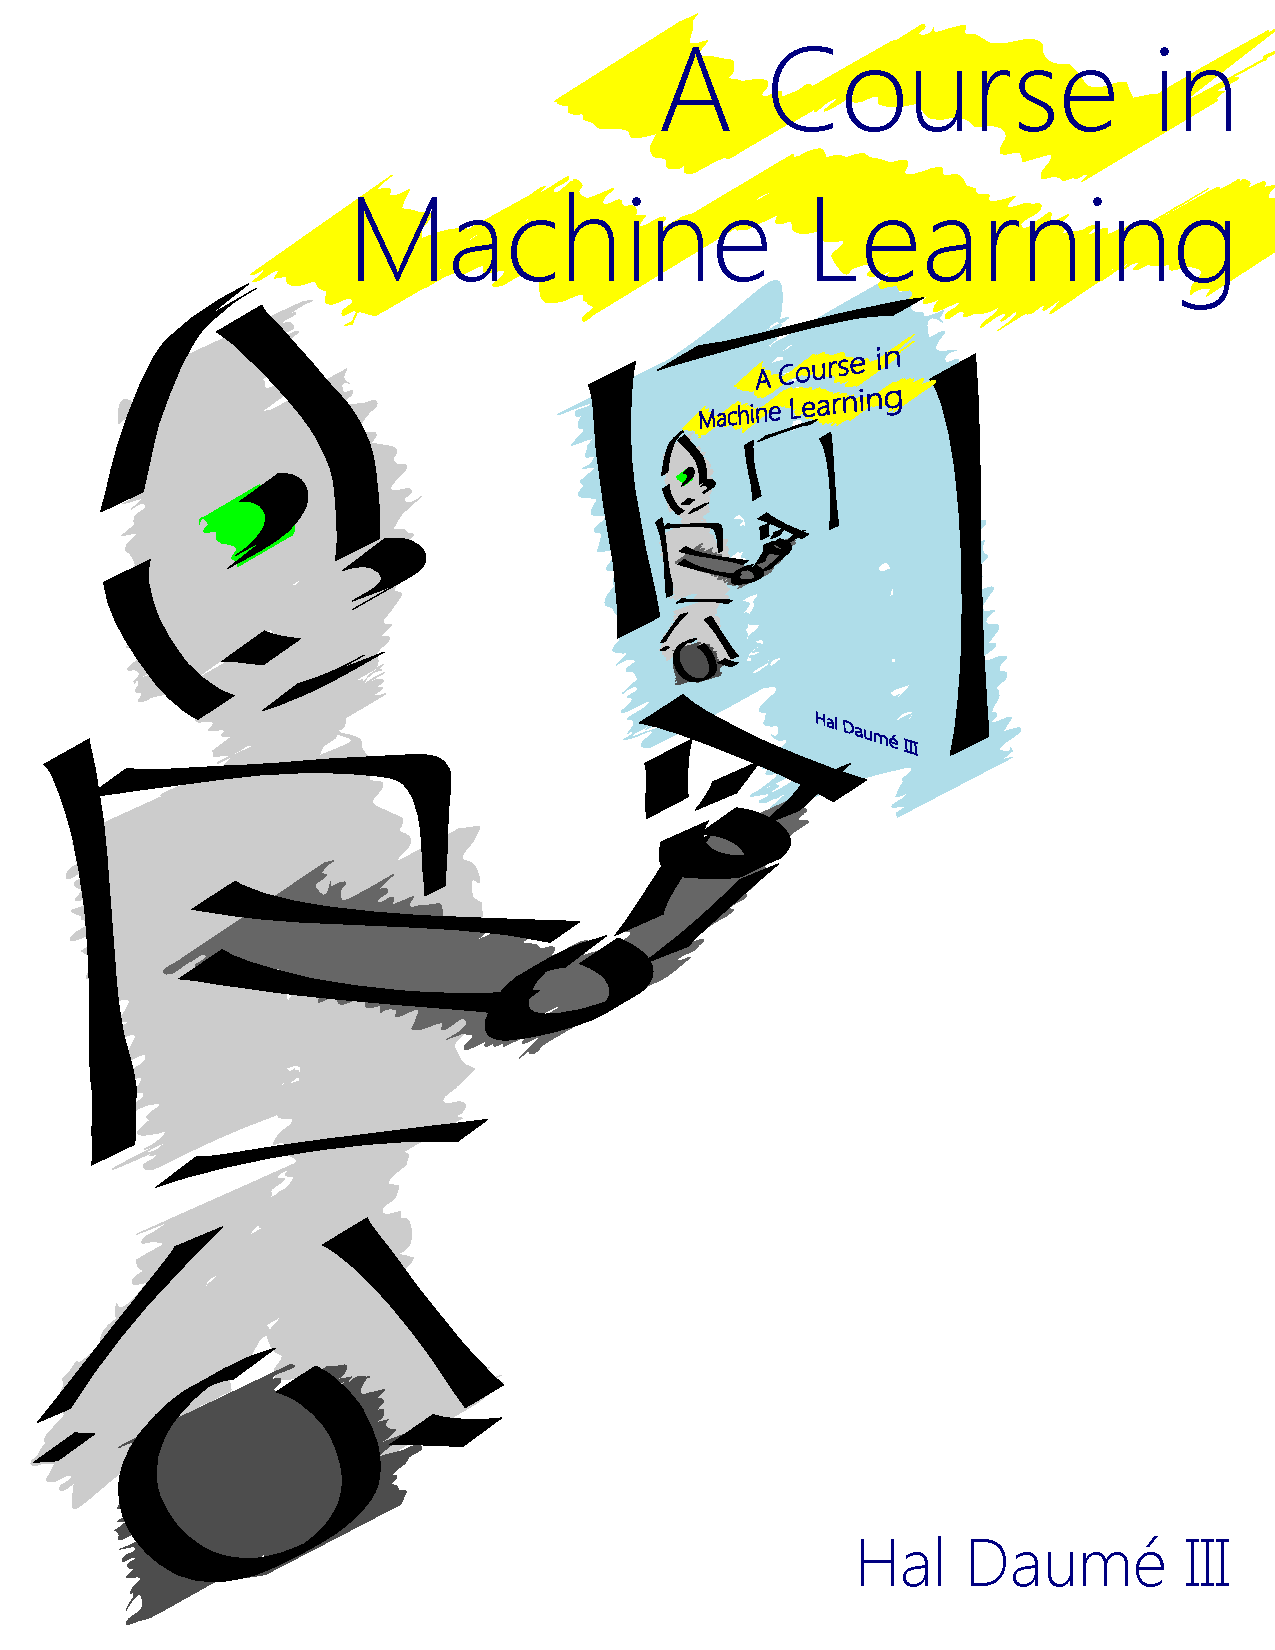
\includepdf[pages={1},frame=true,fitpaper=true,noautoscale,width=614.295pt,height=794.97pt]{cover/cover.pdf}
\maketitle

%\SetWatermarkText{\shortstack[c]{Draft:\\Do Not\\Distribute}}

%\newpage
\begin{fullwidth}
~\vfill
\thispagestyle{empty}
\setlength{\parindent}{0pt}
\setlength{\parskip}{\baselineskip}
Copyright \copyright\ 2013--\the\year\ \thanklessauthor

\par\textsc{Self-published}

\par\bookurl

\par \TODO.\index{license}

\par\textit{Second printing, \monthyear}
\end{fullwidth}

%\newpage
\thispagestyle{empty}
~\vfill
\begin{doublespace}
\noindent%\fontsize{18}{22}\selectfont\itshape
\ttfsegoeuil
\nohyphenation
For my students and teachers.

Often the same.
\end{doublespace}
\vfill
\vfill

\tableofcontents
\listoffigures
\listoftables
\cleardoublepage
%%% Local Variables: 
%%% mode: latex
%%% TeX-master: "courseml"
%%% End: 

\chapter{About this Note} \label{sec:intro}

Note that most of symbols in this note are vector, matrix, or tensor.
Strictly speaking, we should write them as bold to differ from scalars.
But for simplification, most bolds of them are ignored in this note.

Also, $\times$ in superscript will leads into overflow in this latex source code.
Therefore, all $\times$ are replaced by $*$ in superscripts.

When there is no possibility for confusion, we write the propability $Pr(W = w)$ where $W$ is the random variable and $w$ is the specific value to the shorthands $P(w)$.

\tododcmmc


\mainmatter

\chapter{NLP with DL}\label{sec:nlp}

\chapternote{Natural Language Processing with Deep Learning}{Stanford CS224n Winter 2019}

\begin{learningobjectives}
	\item Word Vector
	\item Calculus Review
	\item RNN \& Language Model
	\item Seq2Seq \& Attention
	\item ConvNet for NLP
	\item Transformer
\end{learningobjectives}

\dependencies{Machine Learning Basic}


\section{Word Vector}

Arguably the most simple word vector, i.e., \concept{one-hot vector}: an $\R^{|V| * 1}$ vector with one $1$ and the rest $0$s.
Note that these one-hot vectors are \concept{orthogonal} (i.e., no similarity/relastionship) and $V$ is a very big vocabulary ($\sim 500k$ words for english).

\sidenotedcmmc{In traditional NLP (before 2013), words are regarded as discrete symbols (\concept{localist} representation) and cannot capture similarity. One-hot vector is an example.}

Another idea: \concept{distributional representation} in modern statistical NLP. A word's meaning is given by the words that frequently appear close-by.
Using some $N$-dim ($N \ll |V|$) space is sufficient to encode all semantics of our language into a dense vector.
Once we get the word embedding matrix where each column is a word vector, we can query the word vector from one-hot representation by treating it as \concept{lookup table} instead of using matrix product.

\Figure{word_analogy}{An example of word analogy of man:woman :: king:?}

To evaluate word vectors, there are two fold: \emph{intrinsic} (directly used, e.g. word analogies/similarity) and \emph{extrinsic} (indirectly used in real task, e.g. Q\&A).
Word vector analygies for  $a:b :: c:\textcolor{red}{d}$ is calculated by cosine similarity as example shown in Fig.~\ref{fig:word_analogy}:

\begin{equation}
d = \arg \max_i \frac{(x_b - x_a + x_c)^\top x_i}{\lVert x_b - x_a + x_c \rVert}
\end{equation}

If we have hundreds of millions of words, it's okay to start the vectors \emph{randomly}.
If there is a \emph{small} ($\le 100,000$) training data set, it's best to just treat the pre-trained word vectors as \emph{fixed}.
In the other hand, if there is a large dataset, then we can gain by \concept{fine tuning} of the word vectors.

\subsection{Word2vec}

Two families of models: \concept{Skip-gram} and \concept{Continuous Bag of Words}.

Idea of \concept{Skip-gram} (predicting context words by a given center word) in  Word2vec\mycite{word2vec}:

\begin{itemize}
	\item a large corpus of text $T$ with a vocabulary $V$
	\item every word is represented by a vector $w \in \mathbb{R}^d$ and start off as a random vector
	\item use the (cosine) similarity of the word vectors for $c$ (center word) and $o$ (context/outside word) to calculate the probability of $o$ given $c$: $p(w_o | w_c)$
	\item adjusting the word vectors to maximize the probability
\end{itemize}

\sidenotedcmmc{Why we use two vectors per word? Make it simpler to calculate the gradient of loss function. Because the center word would be one of the choices for the context word and thus squared terms are imported. Average both vectors at the end is the final word vector.}

The conditional probability is calculated by the \concept{softmax} (normalize to probability distribution) of \concept{cosine} similarity (review dot product: $\bm{a} \cdot \bm{b} = |\bm{a}||\bm{b}| \cos\left<\bm{a}, \bm{b}\right>$).
Note that the visualization of word vectos utilizes 2D projection (e.g. PCA) that will loss huge information.

\begin{equation}
p(w_o | w_c) = \frac{\exp(u_o^\top v_c)}{\sum_{w \in V}(u_w^\top v_c)}
\end{equation}
where $v_c$ denotes the center word vector of $w$ when $w$ is used as a center word in the formula, and $u_w$ denotes the context word vector of $w$ as the similar way.
A demo of the window size and conditional probability is shown in Fig.~\ref{fig:word2vec:window_cond}.

\MoveNextFigure{+5cm}
\Figure{word2vec:window_cond}{A demo of the window size and $p(w_o | w_c)$}


The objective function (a.k.a loss or cost function) is given by the (average) negative log likelihood (abbr. \concept{NLL}).
The parameters of the model are adjusted by minimizing the loss function $J(\theta)$ or maximizing the likelihood.
This is, give a high probability estimate to those words that occur in the context and low probability to those don't typically occur in the context.


\begin{align}
	\arg\max_\theta L(\theta) &= \prod_{c=1}^{T} p(w_{c-m}, \cdots, w_{c-1}, w_{c+1}, \cdots, w_{c+m} | w_c; \theta) \nonumber \\
	&= \prod_{c=1}^{T} \prod_{\substack{-m \le j \le m \\ o = j + c \\ o \ne c}} p(w_o | w_c; \theta) \nonumber \\
	&\Downarrow \nonumber \\
	\arg\min_\theta -\frac{1}{T} \log L(\theta) &= -\frac{1}{T} \sum_{c=1}^{T} \sum_{ \substack{-m \le j \le m \\ o=j+c \\ o \ne c}} \log p(w_o | w_c; \theta) \nonumber \\
	&= -\frac{1}{T} \sum_{c=1}^{T} \sum_{ \substack{-m \le j \le m \\ o=j+c \\ o \ne c}} \left( u_o^\top v_c - \log \sum_{w \in V} \exp(u_w^\top v_c)\right) 
	\label{eq:word2vec_loss}
\end{align}
where $m$ is the window size, $\theta \in \mathbb{R}^{2d|V|}$ represents all model parameters.
And we assume that $p(\cdot | w_c)$ are \concept{i.i.d}.

\sidenotedcmmc{The properties of $\log$ and $\arg \max$ ($\arg \min$) used in Eq.~\ref{eq:word2vec_loss} are VERY useful. $\exp(\cdot)$ ensures anything positive.}

We use \concept{gradient descent} (i.e. averaged gradient of all samples/windows) to optimize the loss function.
Note that stochastic (one sample/window with noisy estimates of the gradients) or mini-batch (a subset of samples/windows with size powered of $2$ such as $64$) gradient descent methods are useful to prevent overfitting and train for large dataset.
Calculating the gradient of the loss function is trivial:

\begin{equation}
\begin{split}
\frac{\partial J}{\partial v_c} &= -\frac{1}{T} \sum_{c=1}^{T} \sum_{ \substack{-m \le j \le m \\ o=j+c \\ o \ne c}} \left(u_o - \sum_{x \in V} \frac{\exp(u_x^\top v_c) u_x}{\sum_w \exp(u_w^\top v_c)}\right) \\
&= -\frac{1}{T} \sum_{c=1}^{T} \sum_{ \substack{-m \le j \le m \\ o=j+c \\ o \ne c}} \left(u_o - \sum_{x \in V} p(w_x | w_c) \cdot u_x \right)
\end{split}
\end{equation}

\begin{equation}
\frac{\partial J}{\partial u_o} = -\frac{1}{T} \sum_{c=1}^{T} \sum_{ \substack{-m \le j \le m \\ o=j+c \\ o \ne c}} \left(v_c - p(w_o | w_c)\right)
\end{equation}

Iteratively update equation (na\"ive version) is given by:

\begin{equation}
\theta^{new} = \theta^{old} - \alpha \nabla_\theta J(\theta)
\end{equation}
where $\alpha$ is the learning size (step size) such as $10^{-3}$.

Note that the summation over $|V|$ ($\sum_{x \in V}$) is very expensive to compute!
For every training step, instead of looping over the entire vocabulary, we can just sample several negative examples!
\concept{negative sampling}: train binary logistic regression instead.
$p(D=1|w_o,w_c)$ denotes the probability when $(w_o,w_c)$ came from the same window pf the corpus data, and $p(D=0|w_o,\tilde{w}_o)$ is the probability given $(w_o,\tilde{w}_o)$ did not come from the same window (i.e. noisy/invalid pair).
Randomly sample a bunch of noise words from the \concept{unigram distribution} raised to the power of $3/4$: $p(w) = \nicefrac{U(w)^{3/4}}{Z}$, where $U(w)$ is the counts for every unique words (i.e. unigram) and $Z$ is the nomalization term.

To avoid high frequence effect of words such as \concept{of} and \concept{the}, one simple way is just lop off the first biggest component in the word vector.
The unigram with power of $3/4$ in word2vec is also a trick to handle the effect, where it decrease how often you sample very common words and increase how often you sample rare words.

The objective function is also come from NLL: 

\begin{equation}
J(\theta) = - \frac{1}{T} \sum_{c=1}^T \sum_{ \substack{-m \le j \le m \\ o=j+c \\ o \ne c}} \left( \log \sigma \left( u_o^\top v_c \right) + \sum_{j \sim p(w)} \left[ \log \sigma \left(-u_j^\top v_c\right) \right] \right)
\end{equation}
where \concept{sigmoid} function is $\sigma(x) = \frac{1}{1 + e^{-x}}$ which can be seen as the 1D (binary) version of softmax and used to output the probability, and $k$ is the number of negative samples such as $5$ and $15$.
Note that according to the symmetric property of sigmoid function we get: $P(D=0|\tilde{w}_j,w_c) = 1 - P(D=1|\tilde{w}_j,w_c) = \sigma \left(-u_j^\top v_c\right)$.

\sidenotedcmmc{Although word2vec model is fairly simple and clean, there are actually many tricks which aren't particularly theoretical.}

\concept{Continuous Bag of Words} (CBOW): predict center word from (bag of) context words.
Similar to Skip-gram, the objective function is formulated as:

\begin{align}
J &= -\frac{1}{T} \sum_{c=1}^{T} \log P (w_c | w_{c-m}, \cdots, w_{c-1}, w_{c+1}, \cdots, w_{c+m}) \\
&= -\frac{1}{T} \sum_{c=1}^{T} \log p (v_c | \hat{u}) \\
&= -\frac{1}{T} \sum_{c=1}^{T} \log \mathop{\textup{softmax}}\limits_{c}(v_c^\top \hat{u}) \\
&= -\frac{1}{T} \sum_{c=1}^{T} (v_c^\top \hat{u} - \log \sum_{j=1}^{|V|} \exp (v_j^\top \hat{u}))
\end{align}
where $\hat{u} = \frac{1}{2m} \sum_{ \substack{-m \le j \le m \\ o=j+c \\ o \ne c}} u_o$


Although word2vec can capture complex patterns beyond word similarity, it has inefficient usage of statistics (i.e. rely on sampling rather than directly use counts of words).

\subsection{HW1}

A simple intro to co-occurrence matrix, SVD, cosine similarity, and some applications (e.g. word analogy) of word2vec.

\subsection{GloVe}
\Figure{cooccurrence_matrix}{An example of co-occurrence matrix with window size of $1$}

Co-occurrence matrix $X \in \mathbb{R}^{|V| * |V|}$ with window size $k$.
Fig.~\ref{fig:cooccurrence_matrix} shows an example.
Note that such matrix is extremely sparse and very high dimensional, and the dimensions of the matrix change very often as new words are added very frequently and corpus changes in size.
We can perform SVD on $X$ to reduce the dimensionality to $25 \sim 1000$-dim.
In addition, there are some hacks to $X$ that transform the raw count introduced by \mycite{rohde2005_hacks}: (1) set upper bound (e.g. $100$) or just ignore them all for the counts of too frequent words, (2) ramped windows that count closer words more. (3) use Pearson correlations instead of counts.
Note that they made some interesting observation in their word vector that the verb (e.g. swim) and the corresponding doer (e.g. swimmer) pairs are roughly \emph{linear components} (e.g. $\bm{v}_{swimmer} - \bm{v}_{swim} = k (\bm{v}_{driver} - \bm{v}_{drive})$).

\tododcmmc{SVD}

Although the aforementioned conventional method has disproportionate importance given to large counts and mainly only capture word similarity, it enjoys the fast training and efficient usage of statistics.
GloVe (\textbf{Glo}bal \textbf{Ve}ctor) \mycite{GloVe} combines the advantages from both of this conventional method (global count matrix factorization) and the DL-based methods (local context window methods) such as word2vec.
It captures global corpus statistics directly.

\Figure{ratio_cooccurrence}{An example of the conditional probabilities and their ratio in GloVe paper.}

Some notations: $X_{ij}$ tabulate the number of times word $j$ occurs in the context of word $i$, $X_i = \sum_{k} X_ik$ is the number of times any word appears in the context of word $i$ i.e., the nomalization denominator.
$P_{ij} = P(j|i) = \nicefrac{X_{ij}}{X_i}$ is the probability that word $j$ appear in the context of word $i$.
The crucial insight is that the \emph{ratios} of co-occurrence probabilities as shown in Fig.~\ref{fig:ratio_cooccurrence} to encode meaning components.
We'd like to leverage the word vectors $w_i, w_j, \tilde{w}_k$ to represent such ratio: $F(w_i, w_j, \tilde{w}_k) = \nicefrac{P_{ik}}{P{jk}}$, where $\tilde{w}$ is a seperate \emph{context} word vector for various \emph{probe words} $k$, instead of the word vector $w$ (similar to center word vector in skip-gram).

We can select a unique choice of $F$ by enforcing a few desiderata (i.e. restrictions).
To fit the demand of the \emph{linear components} and the output \emph{scalar} value, in addition to the \emph{homomorphism}
between the groups $(\mathbb{R}, -)$ and $(\mathbb{R}^+, \div)$ (i.e., $F(i,j) = \nicefrac{P_{ik}}{P{jk}} = \nicefrac{1}{F(j,i)} = \nicefrac{P_{jk}}{P{ik}}$), we can derivate that $F(w_i, w_j, \tilde{w}_k) = F\left((w_i - w_j)^\top \tilde{w}_k\right) = \nicefrac{F(w_i^\top \tilde{w}_k)}{F(w_j^\top \tilde{w}_k)} = \nicefrac{P_{ik}}{P_{jk}}$.
Therefore, $F=\exp, w_i^\top \tilde{w}_k = \log(P_{ik}) = \log (X_{ik}) - \log (X_i)$.
Note that the symmetry property of co-occurrence: $X_{ik} = X_{ki}$.
We add two biases to restore the symmetry: $w_i^\top \tilde{w}_k + b_i + \tilde{b}_k = \log (X_{ik})$, where we can analogy that $b_i + \tilde{b}_j = \log X_{i}$.

More details, the relationship to the "global skip-gram" and the complexity refer to the original GloVe paper~\mycite{GloVe}.

\sidenotedcmmc{To handle the ill-defined $\log$ function when its argument be $0$ (its common that $X_{ij}=0$), the authors use the factorized log: $\log(X_{ik}) \rightarrow \log (1+X_{ik})$.}

\begin{align}
w_i \cdot w_j &= \log P(i|j) \\
w_x \cdot (w_a - w_b) &= \log \frac{P(x|a)}{P(x|b)}
\end{align}

Therefore, the ratios of co-occurrence probabilities is the \concept{log-bilinear model with vector differences}.
The final objective function is \emph{weighted} \concept{least squares} (MSE) for this regression problem.

\begin{equation}
	J = \sum_{i,j=1}^V f(X_{ij})\left(w_i^\top \tilde{w}_j + b_i + \tilde{b}_j - 
	log X_{ij}\right)
\end{equation}
where weighted function (is also a hyperparamter) is:

\begin{equation}
f(x) =
\begin{cases}
	\left(\frac{x}{x_{max}}\right)^\alpha & \text{if } x < x_{max} \\
	1 & \text{otherwise}
\end{cases}
\end{equation}
where $x_{max} = 100, \alpha = \nicefrac{3}{4}$ (\emph{empirical} value). 

\subsection{Word sense ambiguity}
Because most words have lots of meanings.
One crude way \mycite{huang-etal-2012-improving} is to cluster word windows around words, retrain with each
word assigned to multiple different clusters $\textsf{bank}_1$, $\textsf{bank}_2$, etc.
Another method \mycite{TACL_word_senses} is weighted sum of different senses of a word reside in a linear superposition, e.g.:

\begin{equation}
v_{\text{pike}} = \alpha_1 v_{\text{pike}_1} + \alpha_2 v_{\text{pike}_2} + \alpha_3 v_{\text{pike}_3}
\end{equation}
where $\alpha_i = \frac{f_i}{\sum_{j=1}^3 f_j}$ for frequency $f$.

The result is counterintuitive very well, because of the idea from \emph{sparse} coding you can actually separate out the senses.

\section{Math Backgrounds}
For \concept{multi-class classification} problem, \concept{NLL} (negative likelihood loss) is the objective function of \concept{Maximum Likelihood Estimate} (abbr, MLE):

\begin{equation}
J(\bm{\theta}) = - \sum_i \log p(y = y^{true}_i | \bm{x}_i; \bm{\theta})
\end{equation}

\concept{cross entropy} (distance measure) between (discrete) distribution $p$ and $q$ is more convenient way:

\begin{equation}
H(p, q) = - \sum_{c=1}^C p(c) \log q(c)
\end{equation}

However, in the multi-class (with single label) setting, the p(c) is the \concept{ground truth distribution} which has the \emph{one-hot} style (\concept{empirical distribution}), i.e. $p = [0, \cdots, 0, 1, 0, \cdots, 0]$ where $1$ at the right class and $0$ everywhere else.
Therefore, the \concept{cross entropy} in the multi-class classification is \emph{equal} to the NLL.

A simple $k$-class model example is \concept{dense layer} with \emph{softmax}:

\begin{equation}
	p(y|\bm{x}; \bm{\theta}) = softmax(\bm{W}_2 f(\bm{W}_1 \bm{x} + \bm{b}))
\end{equation}
where $\bm{\theta} = [\bm{W}_1, \bm{b}, \bm{W}_2]^\top $ are the parameters, $\bm{x} \in \mathbb{R}^m, \bm{W}_1 \in \mathbb{R}^{n * m}, \bm{b} \in \mathbb{R}^n, \bm{W}_2 \in \mathbb{R}^{k * n}$, $f(\cdot)$ is a kind of simple activate (non-linear) function to provide non-linearity, such as $ReLU(x) = max(0, x)$.
The visualization of neural network refer to \sidenote{ ConvNetJS: \url{https://cs.stanford.edu/people/karpathy/convnetjs/demo/classify2d.html}}.

The \concept{Jacobian Matrix} (generalization of the gradient) of function $\bm{f}(\bm{x}): \mathbb{R}^n \rightarrow \mathbb{R}^m$ is a $m \times n$ matrix: $\left(\frac{\partial \bm{f}}{\partial \bm{x}}\right)_{ij} = \frac{\partial f_i}{x_j}$.

Supposed that we have a function $\bm{g}(\bm{f}(x)), \bm{f}: \mathbb{R} \rightarrow \mathbb{R}^2, \bm{g}: \mathbb{R}^2 \rightarrow \mathbb{R}^2$, we can compute the partial derivative of $\bm{g}$ w.r.t $x$ by \concept{chain rule}:

\begin{equation}
	\frac{\partial \bm{g}}{\partial x} = \begin{bmatrix}
	\frac{\partial g_1}{\partial f_1} \frac{\partial f_1}{x} + \frac{\partial g_1}{\partial f_2} \frac{\partial f_2}{x}\\
	\frac{\partial g_2}{\partial f_1} \frac{\partial f_1}{x} + \frac{\partial g_2}{\partial f_2} \frac{\partial f_2}{x}
	\end{bmatrix}
\end{equation}

\sidenotedcmmc{$\frac{d g_1}{d \bm{y}} = \frac{\partial g_1}{y_1} + \frac{\partial g_2}{y_2}$ is the relationship of the full differential and the partial differential.}

It is the same as multiplying the two Jacobians:

\begin{equation}
\frac{\partial \bm{g}}{\partial x} = \frac{\partial \bm{g}}{\partial \bm{f}} \frac{\partial \bm{f}}{\partial x} = \begin{bmatrix}
\frac{\partial g_1}{\partial f_1} & \frac{\partial g_1}{\partial f_2} \\
\frac{\partial g_2}{\partial f_1} & \frac{\partial g_2}{\partial f_2}
\end{bmatrix} \begin{bmatrix}
\frac{\partial f_1}{\partial x} \\
\frac{\partial f_2}{\partial x}
\end{bmatrix}
\end{equation}

There are some useful identities:

\begin{itemize}
	\item $\frac{\partial \bm{x}}{\partial \bm{x}} = \bm{I}$
	\item $\frac{\partial \bm{Wx}}{\partial \bm{x}} = \bm{W}, \frac{\partial \bm{u}^\top \bm{x}}{\partial \bm{x}} = \bm{u}^\top$
	\item $\frac{\partial \bm{x^\top W}}{\partial \bm{x}} = \bm{W^\top}$
	\item For elemenwise function $\bm{f}(\bm{x})$: $\frac{\partial \bm{f}}{\partial \bm{x}} = \texttt{diag}(\bm{f}^\prime(\bm{x}))$
	\item $\frac{\partial \bm{\theta}^\top (\bm{W} \cdot \bm{h})}{\partial \bm{W}} = \bm{\theta} \bm{h}^\top$ where $\bm{\theta} \in \mathbb{R}^{D_\theta * 1}, \bm{W} \in \mathbb{R}^{D_\theta * D_h}, \bm{h} \in \mathbb{R}^{D_h * 1}$
	\item For cross entropy loss: $J(\bm{h}) = - \bm{y}^\top \log (\hat{\bm{y}}) = - \bm{y}^\top \log \texttt{softmax}(\bm{h})$ ($\bm{y}$ is one-hot vector) is: $\frac{\partial J}{\partial \bm{h}} = (\hat{\bm{y}} - \bm{y})^\top$
\end{itemize}

We can use \concept{backward propagation} (reversed of the \emph{topological sort}) and \emph{re-use} intermediate nodes to reduce complexity in the \emph{computation graph}.

Other machine learning basic concepts are: \concept{regularization} (e.g. L2) to prevent \concept{overfitting}, vectorization to parallelization, (non-linear) \concept{activation function} (e.g. sigmoid, tanh, (leaky) ReLU), parameter initialization (e.g. Xavier), \concept{Optimizer} (e.g. RMSprop, Adam), learning rate.

\sidenotedcmmc{Compared with activations such as sigmoid and tanh, ReLU does not \emph{saturate} even for larger values. Note that ReLU is not \emph{differentiable} at $0$, where we can use \emph{sub-derivatives} in implementation with a certain value such as $0$ or $1$.}

\subsection{Data Preprocessing}
\Figure{mean_subtraction}{An exmaple of mean subtration.}
\Figure{normalization}{An example of normalization.}

\begin{itemize}
	\item \textbf{Mean Subtraction (Shifting)}: Shifting all data so that they have zero mean as shown in Fig.~\ref{fig:mean_subtraction}. Formally, $\bm{x}^{(i)} \leftarrow \bm{x}^{(i)} - \mathbb{E}[\bm{x}^{(i)}]$ for sample $i$, where $\mathbb{E}$ indicates mean.
	\item \textbf{Normalization (Scaling)}: Scale every input feature dimension to have
	similar ranges of magnitudes, as shown in Fig.~\ref{fig:normalization}. This is useful since input features are often measured in different "units", but we often want to initially consider all features as equally important. Formally, $x^{(i)}_{j} \leftarrow \frac{x^{(i)}_{j}}{\sigma_i (x^{(i)}_{j})}$ for feature $j$ in sample $i$ where $\sigma(\cdot)$ is the standard variance over $x^{(0)}_{j}, \cdots, x^{(N)}_{j}$.
	\item \textbf{Whitening}: Whitening converts the data to a have an identity covariance matrix - that is, features become uncorrelated and have a variance of $1$. In the specific, we can divide the principal components achieved from PCA by the square roots of their eigenvalues (singular value).
\end{itemize}

\subsection{Parameter Initialization}
	
If two hidden units have exactly the same bias and exactly the same incoming and outgoing weights (e.g. different channels for learning different features in the same convolutional layer), they will always get exactly the same gradient.
So we should initialize the weights to small random values.

A good starting strategy is to initialize the weights to small random numbers of \concept{normal distribution} with the mean around $0$.
Xavier et al. \mycite{Xavier} suggest that for sigmoid and tanh activation units, it's better for the weight matrix $W \in \mathbb{R}^{n^{(l+1)} * n^{(l)}}$ to be initialized randomly with a \concept{uniform distribution}:
\begin{equation}
W \sim U\left[- \sqrt{\frac{6}{n^{(l)} + n^{(l+1)}}}, \sqrt{\frac{6}{n^{(l)} + n^{(l+1)}}}\right]
\end{equation}
where $n^{(l)}, n^{(l+1)}$ are also called \textbf{fan-in} and \textbf{fan-out}.
Besides, bias units are initialized to $0$.

\subsection{Optimizer}
To avoid a diverging loss (too large learning step) or unconverging (too small learning step), there are some learning strategies.

\concept{Annealing}: start off with a high learning rate to approach a minimum quickly, after several iterations, the learning rate is reduced in some way under a more fine-grained scope.
\begin{itemize}
	\item Exponential decay: $\alpha(t) = \alpha_0 e^{-kt}$ where $\alpha_0$ is initial learning rate.
	\item Decrease over time: $\alpha(t) = \nicefrac{(\alpha_0 \tau)}{\max(t, \tau)}$ where $\tau$ denotes the time at which the learning rate should start reducing.
\end{itemize}

\Figure{momentum}{A picture of momentum.}

\concept{Momentum} (a picture of it can be seen in Fig.\ref{fig:momentum}) based methods:
\begin{itemize}
	\item AdaGrad: $\bm{m} \leftarrow \bm{m} + \left(\nabla_{\bm{\theta}} J (\bm{\theta})\right)^2, \bm{\theta} \leftarrow \bm{\theta} - \alpha \nabla_{\bm{\theta}} J (\bm{\theta}) \odot \left(\sqrt{\bm{m}} + \epsilon\right)^{-1}$ where $\odot, (\cdot)^{-1}, (\cdot)^{2}, \sqrt{\cdot}$ are all element-wise operators, and $\epsilon$ is a very small value such as $10^{-8}$ to prevent \concept{arithmetic underflow}.
	It leads to that parameters that have not been updated much in the past are likelier to have higher learning rates now.
	\item RMSprop: $\bm{m} \leftarrow \beta \bm{m} + (1-\beta) \left(\nabla_{\bm{\theta}} J (\bm{\theta})\right)^2, \bm{\theta} \leftarrow \bm{\theta} - \alpha \nabla_{\bm{\theta}} J (\bm{\theta}) \odot \left(\sqrt{\bm{m}} + \epsilon\right)^{-1}$ where $\beta$ is the decay rate with default value $0.9$. Unlike AdaGrad, its updates do not become monotonically smaller.
	\item Adam\mycite{Adam}: $\bm{m} \leftarrow \beta_1 \bm{m} + (1-\beta_1) \nabla_{\bm{\theta}} J (\bm{\theta}), \bm{v} \leftarrow \beta_2 \bm{v} + (1-\beta_2) \left(\nabla_{\bm{\theta}} J (\bm{\theta})\right)^2, \hat{\bm{m}} = \bm{m} / (1 - \beta_1^t), \hat{\bm{v}} = \bm{v} / (1 - \beta_2^t), \bm{\theta} \leftarrow \bm{\theta} - \alpha \hat{\bm{m}} /  \left(\sqrt{\hat{\bm{v}}} + \epsilon\right)^{-1}$, where $/$ is also a element-wise operator, hyperparameters $\beta_1 = 0.9, \beta_2 = 0.999 \in [0, 1)$. $\hat{\bm{m}}, \hat{\bm{v}}$ are the bias-corrected $\bm{m}, \bm{v}$, and they indicate a rolling average
	of the gradients and a rolling average of the magnitudes of the gradients, respectively. In adition, $\bm{m}, \bm{v}$ are all initialized to $\bm{0}$ Adam is like a combination of RMSProp and momentum.
\end{itemize}

\sidenotedcmmc{For the implementation of momentum such as RMSprop, there is a interesting small trick: use $\bm{m} = \bm{m} - (1-\beta)(\bm{m} - \left(\nabla_{\bm{\theta}} J (\bm{\theta})\right)^2)$ instead of $\bm{m} = \beta \bm{m} + (1-\beta) \left(\nabla_{\bm{\theta}} J (\bm{\theta})\right)^2$. In such way, we need calculate only one multiplication, compared with original two multiplications.}

\subsection{Regularization}
\textbf{1. Dropout}

During training, \concept{dropout} \mycite{dropout} randomly disables units in the hidden layer by a mask vector drawn from Bernoulli distribution where each entry is $0$ with probability $p_{\text{drop}}$ and $1$ with probability ($1 − p_{\text{drop}}$):
\begin{equation}
\text{Dropout Layer: } \textcolor{red}{d_i \sim \text{Bernoulli}(1 - p_{\text{drop}}), \hat{\bm{h}}^{(t)} = } \textcolor{blue}{\frac{1}{1-p_{\text{drop}}}} \textcolor{red}{\bm{d} \odot \bm{h}^{(t)}}
\end{equation}
where $\odot$ is element-wise product, $\bm{d} \in \{0, 1\}^{D_h}, \bm{h}^{(t)} \in \mathbb{R}^{D_h}$.

If the expected output of a neuron during testing if far different as it was during training, the magnitude of the outputs could be radically different, and the behavior of the network is no longer well-defined.
Therefore, all the parameters should divided by retain rate $1-p$ (blue part in above formula), so that $\mathbb{E}_{p_{\text{drop}}} [\bm{h}_{\text{drop}}]_i = h_i$.
If we do not such correction in training, we should multiply $1-p$ to all related parameters.

If we use dropout in testing, the result is \emph{unstable} (vary from every testing) because of the
dropout is drawn from Bernoulli distribution.
Therefore, we should apply dropout only during training but not during evaluation or testing.

\textbf{2. Batch Normalization}

Although \concept{batch nomalization} \mycite{BatchNorm} is like nomalization used in data preprocessing with $N$ be the mini-batch size instead of the dataset size, it is inserted between hidden layers to normalize the output of last layer.
It leads to achieve the fixed distributions of inputs that would remove the ill effects of the internal covariate shift.
\emph{Internal Covariate Shift} is defined as the change in the distribution of network activations due to the change in network parameters during training.

The batch normalization in training is defined as follows:
\begin{equation}
\text{BN}(h_i) = \gamma \frac{h_i - \mu_{\mathcal{B}}}{\sqrt{\sigma_{\mathcal{B}}^2 + \epsilon}} + \beta
\end{equation}
where $\gamma, \beta$ are \concept{trainable parameters}, $\mu_{\mathcal{B}}, \sigma_{\mathcal{B}}^2$ are the mean and variance over the mini-batch as the way of normalization for data preprocessing.
Since the mean subtraction will \emph{ignore} the learned bias which may useful to the model.
The trainable $\gamma$ and $\beta$ are used to corrected them and make the BN layer trainable.
Them ensure that the batch normalization inserted in the network can represent the identity transform.

However, when testing, we cannot use mini-batch in most time.
We instead feed one sample into the model.
Therefore, we leverage $m$ training mini-batches to perform \concept{unbiased estimates} of them:
\begin{align}
&\mathbb{E}[h_i] \leftarrow \mathbb{E}_{\mathcal{B}}[\mu_{\mathcal{B}}] \nonumber \\
&\texttt{Var}[h_i] \leftarrow \frac{m}{m-1} \mathbb{E}_{\mathcal{B}}[\sigma_{\mathcal{B}}^2] \nonumber
\end{align}

Note that in many implementations, the above estimation is replaced with the way like the momentum used in RMSprop.
More details refer to the source code, e.g. Keras.

\subsection{Practice: Named Entity Recognition}
To find and classify words as entities (e.g. location, or organization) in text.
One simple idea is that train softmax classifier to classify a center word by taking
\emph{concatenation} of word vectors surrounding it in a window (\emph{word window}) \mycite{NER_ICML}.
To perform NER of localtion, we need (unnormalized) score for each window, and make \emph{true window}’s (i.e. location in the center) score larger and other \emph{corrupt window}’s score lower.
The model is formulated as:

\begin{equation}
s = \bm{W}_2 f(\bm{W}_1 \bm{x} + \bm{b})
\end{equation}


The objective function (\emph{max-margin loss}) is:

\begin{equation}
J = max(0, s_c - (s - 1))
\end{equation}
where $s$ and $s_c$ is the score of true window and corrupt window.
It ensure each window with an NER location at its center should have a score $+1$ higher than any window without a location at its center.

\subsection{HW2}

Gradient calculation and implementation of word2vec.

\textbf{1. Written: Understanding word2vec}
\begin{align*}
	&(a) \ \hat{y}_o = P(O = o | C = c) \\
	&(b) \ \frac{\partial J}{\partial \bm{v}_c} = (\hat{\bm{y}} - \bm{y})^\top \bm{U}^\top \\
	&(c) \ \frac{\partial J}{\partial \bm{U}} = \bm{v}_c (\hat{\bm{y}} - \bm{y})^\top \\
	&(d) \ \sigma (\bm{x}) = \frac{1}{1 + \exp (- \bm{x})}, \frac{d \sigma (\bm{x})}{\bm{x}} = \texttt{diag} (\sigma (x_i) (1 - \sigma (x_i))) \\
	&(e) \ \frac{\partial J}{\partial \bm{v}_c} = \sum_k \sigma (\bm{u}_k^\top \bm{v}_c) \bm{u}_k^\top - (1 - \sigma (\bm{u}_o^\top \bm{v}_c)) \bm{u}_o^\top \\
	& \ \frac{\partial J}{\partial \bm{u}_o} = (\sigma (\bm{u}_o^\top \bm{v}_c) - 1) \bm{v}_c^\top \\
	& \ \frac{\partial J}{\partial \bm{u}_k} = \sigma (\bm{u}_k^\top \bm{v}_c) \bm{v}_c^\top \\
	&(f) \ (i) \frac{\partial J}{\partial \bm{U}} = \sum_o \bm{v}_c (\hat{\bm{y}}_o - \bm{y}_o)^\top \\
	&(ii) \frac{\partial J}{\partial \bm{v}_c} = \sum_o (\hat{\bm{y}}_o - \bm{y}_o)^\top \bm{U}^\top \\
	&(iii) \frac{\partial J}{\partial \bm{v}_w} = \bm{0}
\end{align*}

\sidenotedcmmc{Use shape convention to check the result.}

\textbf{2 Coding: Implementing word2vec}

Note that $\bm{U}, \bm{V}$ in the handout are the matrices whose $i$-th column is the $n$-dimensional embedded vector for word $w_i$.
However, in the codes of HW2, all the centerWordVectors and outsideVectors are as rows.

\section{Dependency Parser}
Two views of linguistic structure: (1) constituency (i.e., phrase structure grammar, or context-free grammar) (2) Dependency structure.
Dependence parse trees (single root with optional fake root, acyclic) use binary asymmetric relations which depicted as typed arrows going from \emph{head} to \emph{dependent}.
Note that the natural language is ambiguity.

Basic transition-based dependency parser \mycite{nivre-2003-efficient} with stack $\sigma = [\text{ROOT}]$, buffer $\beta = w_1, \cdots, w_n$, set of dependency arcs $A = \emptyset$, and a set of actions (\emph{transitions}) based on the above $3$-tuple:
\begin{align}
&\text{1. Shift: } \sigma , w_i | \beta, A \Rightarrow \sigma | w_i, \beta, A \nonumber \\
&\text{2. Left-Arc reduction: } \sigma | w_i | w_j, \beta, A \Rightarrow \sigma | w_j, \beta, A \cup \{r(w_j, w_i)\} \nonumber \\
&\text{3. Right-Arc reduction: } \sigma | w_i | w_j, \beta, A \Rightarrow \sigma | w_i, \beta, A \cup \{r(w_i, w_j)\} \nonumber
\end{align}
where $r(w_j, w_i)$ denotes $w_i$ is the dependency of $w_j$ (e.g. $\text{nsubj}(\text{ate} \rightarrow \text{I})$), $|$ and $\cup$ stand for concatenate.
The finish state is: $\sigma = [w], \beta = \emptyset$.
How to select (search) the best choice among the exponential size of different possible parse trees is the problem.
In 1960s, they use \emph{dynamic programming algorithms} ($\mathcal{O}(n^3)$).
In paper \mycite{nivre-2003-efficient}, the authors predict each action by a discriminative classifier (e.g. SVM classifier) which is more efficient but the accuracy is fractionally below the state-of-the-art.

\subsection{Neural Dependency Parsing}
Compared with traditional sparse feature-based discriminative dependency parsers, the work by \mycite{chen-manning-2014-fast} utilizes \concept{feedforward neural network model} with simple \concept{dense layers} and the softmax layer to predict each transition.
The input features with embedding dimension $d$ are:

\begin{enumerate}
	\item $x^{w} \in \mathbb{R}^{d * N_w}$: The top $3$ words on the stack and buffer $s_1, s_2, s_3, b_1, b_2, b_3$; the first and second leftmost / rightmost children of the top two words on the stack $lc_1(s_i), rc_1(s_i), lc_2(s_i), rc_2(s_i), i = 1, 2$; the
	leftmost of leftmost / rightmost of rightmost children of the top two words on the stack $lc_1(lc_1(s_i)), rc_1(rc_1(s_i)), i = 1, 2$; In total, $N_w = 18$.
	\item $x^{t} \in \mathbb{R}^{d * N_t}$: The corresponding POS (Part-of-speech, e.g. noun, verb, adjective) tags for $S_{word}$, $N_t = 18$.
	\item $x^{l} \in \mathbb{R}^{d * N_l}$:  The corresponding arc labels of words, excluding those $6$ words on the stack/buffer, $N_l = 12$.
\end{enumerate}

\sidenotedcmmc{Note that we use a special \textbf{NULL} token for non-existent elements: when the stack and buffer are empty or dependents have not been assigned yet.}

The predicted class is the one of transitions (i.e. shift, left/right arc reduction): $p = \texttt{softmax}(\bm{W}_2 f(\bm{W}_1^w \bm{x}^w + \bm{W}_1^t \bm{x}^t + \bm{W}_1^l \bm{x}^l + \bm{b}_1) + \bm{b}_2)$, where $f(\cdot)$ is the activation function (e.g. ReLU, or $x^3$).
The number of class is $3$ when untyped reductions or $T * 2 + 1$ when typed reductions (e.g. left-arc reduction with type \emph{nsubj}).

\subsection{HW3}
\textbf{1. Machine Learning \& Neural Networks}

\begin{enumerate}[label=(\alph*)]
	\item Adam
	\begin{enumerate}[label=(\roman*)]
		\item Because $\beta = 0.9$, most of the final gradients ($\bm{m}$) come from the past ($90\%$). Even if current gradients are varying much from previous, it only occupy $1 - \beta_1 = 0.1$ of the final gradients.
		\item Parameters that have not been updated much in the past are likelier to have higher learning rates.
	\end{enumerate}
	\item Dropout
	\begin{enumerate}[label=(\roman*)]
		\item If the expected output of a neuron during testing if far different as it was during training, the magnitude of the outputs could be radically different, and the behavior of the network is no longer well-defined. Thus, all the parameters should divided by retain rate $1-p$, so that $\mathbb{E}_{p_{\text{drop}}} [\bm{h}_{\text{drop}}]_i = h_i$.
		\item If we use dropout in testing, the result is unstable because of the dropout is drawn from Bernoulli distribution.
	\end{enumerate}
\end{enumerate}

\textbf{2. Neural Transition-Based Dependency Parsing}

(a) The remaindered configuration is:
\begin{table}
	\begin{center}
		\begin{tabular}{c|c|c|c}
			Stack & Buffer & New dependency & Transition \\
			\hline
			[ROOT, parsed, this] & [sentence, correctly] & & \textsf{SHIFT} \\ \hline
			[ROOT, parsed, this, sentence] & [correctly] & & \textsf{SHIFT} \\ \hline
			[ROOT, parsed, sentence] & [correctly] & sentence $\rightarrow$ this & \textsf{LEFT-ARC} \\ \hline
			[ROOT, parsed] & [correctly] & parsed $\rightarrow$ sentence & \textsf{RIGHT-ARC} \\ \hline
			[ROOT, parsed, correctly] & [] & & \textsf{SHIFT} \\ \hline
			[ROOT, parsed] & [] & parsed $\rightarrow$ correctly & \textsf{RIGHT-ARC} \\ \hline
			[ROOT] & [] & ROOT $\rightarrow$ parsed & \textsf{RIGHT-ARC}
		\end{tabular}
	\end{center}
\end{table}

(b) $2n$

Note that in the source code, the restriction that the version of PyTorch must be 1.0.0 is meaningless and thus I remove it.

\section{Language Modeling and Recurrent Neural Networks}

Language Modeling: given a sequence of words $\bm{x}^{(1)}, \cdots, \bm{x}^{(t)}$, compute the probability distribution of the next word at $\bm{x}^{(t+1)}$:
\begin{equation}
P(\bm{x}^{(t+1)} | \bm{x}^{(1)}, \cdots, \bm{x}^{(t)})
\end{equation}

The joint probability of a text is:
\begin{equation}
P(\bm{x}^{(1)}, \cdots, \bm{x}^{(T)}) = \prod_{t=1}^T P(\bm{x}^{(t)} | \bm{x}^{(t-1)}, \cdots, \bm{x}^{(1)})
\end{equation}

$n$-gram is a chunk of $n$ consecutive words: unigram, bigram, trigram, 4-gram, ...
$n$-gram language model is based on a simplifying assumption: $\bm{x}^{(t+1)}$ depends only on the preceding $n-1$ words with i.i.d.:
\begin{align}
P(\bm{x}^{(t+1)} | \bm{x}^{(t)}, \cdots, \bm{x}^{(1)}) &= P(\bm{x}^{(t+1)} | \bm{x}^{(t)}, \cdots, \bm{x}^{(t-n+2)}) \nonumber \\
&= \frac{P(\bm{x}^{(t+1)}, \bm{x}^{(t)}, \cdots, \bm{x}^{(t-n+2)})}{P(\bm{x}^{(t)}, \cdots, \bm{x}^{(t-n+2)})} \nonumber
\end{align}
where the $n$-gram and (n-1)-gram probabilities are calculated by \emph{counting}.
There are some \emph{sparsity problems} with the above $n$-gram models such as the numerator or denominator is zero.
Some tricks such as \emph{smoothing} (add small $\delta$ to the count) and \emph{backoff} (e.g. $4$-gram backoff to $3$-gram) are proposed to solve them.

\begin{figure}[!thp]
	\centerline{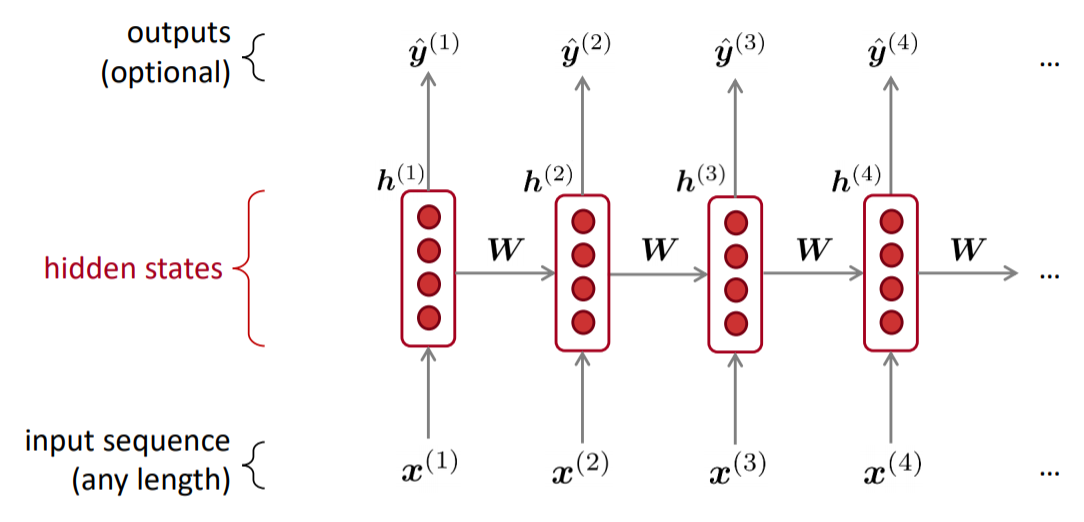
\includegraphics[width=8.0cm]{figs/RNN.png}}
	\caption{Principle of RNN}
	\label{RNN}
\end{figure}

\sidenotedcmmc{Note that for $n$-gram, increasing $n$ makes sparsity problems worse. Typically $n \le 5$.}

To process \emph{variable} length \concept{sequential input} such as text, \concept{Recurrent Neural Network} (RNN) is introduced.
As the principle of RNN shown in Fig.~\ref{RNN}: \emph{repeat} (i.e. \concept{unfold} or unroll) the same RNN cell for each time-step but with different input and previous \concept{hidden state}.
A vanilla RNN for language modeling is:
\begin{align}
\bm{h}^{(t)} &= \sigma \left(\bm{W}_h \bm{h}^{(t-1)} + \bm{W}_x \bm{x}^{(t)} + \bm{b}_1\right) \nonumber \\
\hat{\bm{y}} &= P(\bm{x}^{(t)} | \bm{x}^{(t-1)}, \cdots, \bm{x}^{(1)}) \nonumber \nonumber \\
&= \texttt{softmax}(\bm{U}\bm{h}^{(t)} + \bm{b}_2) \nonumber
\end{align}
where $\sigma(\cdot)$ is the activation function, and $\bm{h}^{(0)}$ is the initial (random or zero) hidden state.
The gradient w.r.t. the weight matrix is the \emph{sum} of the gradients w.r.t each time it appears using \concept{back-propagation through time} (BPTT, just as same as normal back-prop).
And the \concept{evaluation metric} for language modeling is \emph{perlexity} which is equal to the exponential of the cross-entropy losses:
\begin{align}
\text{perplexity} &= \prod_{t=1}^T \left(\frac{1}{P_{LM} (\bm{x}^{(t+1)} | \bm{x}^{(t)}, \cdots, \bm{x}^{(1)})}\right)^{\nicefrac{1}{T}} \nonumber \\
&= \exp\left(\frac{1}{T} \sum_{t=1}^T -\log \hat{\bm{y}}^{(t)}\right)
\end{align}

There are some other applications of RNN: part-of-speech tagging, named entity recognition, sentence classification, text generator, encoder module, etc.
The final feature can be the final hidden state or elemen-wise max/mean of all hidden states.
Using chain rule, we get $\frac{\partial J^{(n)}}{\partial \bm{h}^{(1)}} = \frac{\partial J^{(n)}}{\partial \bm{h}^{(n)}} \times \prod_{i=2}^n \frac{\partial \bm{h}^{(n)}}{\partial \bm{h}^{(n-1)}} = \frac{\partial J^{(n)}}{\partial \bm{h}^{(n)}} \times \prod_{i=2}^n \sigma^\prime \circ \bm{W}_h$.
For a large $n$ and small $\bm{W}_h$, it's easy to encounter the vanishing gradient problem.
In overall, the \emph{vanilla} RNN has these disadvantages: (1) recurrent computation is slow (2) hard to access long-term information (\concept{long-term dependencies}) due to \emph{gradient vanish} and \emph{gradient explosion}.

We can formalize the above vanishing intuitions according to \mycite{RNN_vanishing}.
Let $\bm{W}_h$ have the \concept{eigenvalues} $\lambda_1, \cdots, \lambda_n$ such that $|\lambda_1| > |\lambda_2| > \cdots > |\lambda_n|$ and the corresponding (left) eigenvectors $\bm{q}_1^\top, \cdots, \bm{q}_n^\top$ which have unit norms: $\bm{q}_i^\top \bm{W}_h = \lambda_i \bm{q}_i$.
We can rewrite the gradients $\frac{J^{(n)}}{\bm{h}^{(n)}} = \sum_{i=1}^N c_i \bm{q}_i^\top$ where $c_i = 0$ for $i < j$ and $c_j \ne 0$.
Thus, the overall gradient is:
\begin{align}
\frac{\partial J^{(n)}}{\partial \bm{h}^{(1)}} &= \frac{\partial J^{(n)}}{\partial \bm{h}^{(n)}} \times \prod_{i=2}^n \sigma^\prime \circ \bm{W}_h \nonumber \\ 
&= \sum_{i=1}^N c_i \bm{q}_i^\top (\texttt{diag}(\sigma^\prime))^{n-1} (\bm{W}_h)^{n-1} \nonumber \\
&= \sum_{i=1}^N c_i \bm{q}_i^\top (\bm{W}_h)^{n-1} (\texttt{diag}(\sigma^\prime))^{n-1} \nonumber \\
&= c_j \lambda_j^{n-1} \bm{q}_j^\top (\texttt{diag}(\sigma^\prime))^{n-1} + \lambda_j^{n-1} \sum_{i=j+1}^N c_i \left(\frac{\lambda_i}{\lambda_j}\right)^{n-1} \bm{q}_i^\top  (\texttt{diag}(\sigma^\prime))^{n-1} \nonumber \nonumber \\
&\approx c_j \lambda_j^{n-1} (\sigma^\prime)^{n-1} \bm{q}_j^\top \nonumber
\end{align}
where $\frac{\lambda_i}{\lambda_j} < 1$, and for large $n$ we have $\lim_{n \to \infty} \left(\frac{\lambda_i}{\lambda_j}\right)^{n-1} = 0$.
Therefore, if $\forall j, \sigma^\prime < \frac{1}{\lambda_j}$ then we get vanishing gradient.
Note that, $\sup \text{sigmoid}^\prime = \frac{1}{4}, \sup ReLU^\prime = 1$.
Thus, the largest eigenvalue $\lambda_1 < \frac{1}{\sigma^\prime}$ will lead to vanishing.

For avoid gradient explosion, one simple method is \emph{gradient clipping}: $\hat{\bm{g}} \leftarrow \frac{threshold}{\lVert \bm{g} \rVert} \bm{g}$ if $\lVert \bm{g} \rVert \ge threshold$.
As for fixing vanishing gradient, many RNN variants are introduced such as \concept{Long Short-Term Memory} (LSTM) \mycite{LSTM} and \concept{Gated Recurrent Unit} (GRU) \mycite{GRU}.
LSTM uses two \emph{separated} memories: \emph{hidden state} $\bm{h}^{(t)}$ for \emph{short-term} information and \emph{cell state} $\bm{c}^{(t)}$ for \emph{long-term} information.
There are three \emph{gates} performed in each LSTM \emph{cell}:
\begin{align}
&\text{Forget gate: } \bm{f}^{(t)} = \sigma(\bm{W}_f \bm{h}^{(t-1)} + \bm{U}_f \bm{x}^{(t)} + \bm{b}_f) \nonumber \\
&\text{Input gate: } \bm{i}^{(t)} = \sigma(\bm{W}_i \bm{h}^{(t-1)} + \bm{U}_i \bm{x}^{(t)} + \bm{b}_i) \nonumber \\
&\text{Output gate: } \bm{o}^{(t)} = \sigma(\bm{W}_o \bm{h}^{(t-1)} + \bm{U}_o \bm{x}^{(t)} + \bm{b}_o) \nonumber \\
&\text{New cell content: } \tilde{\bm{c}}^{(t)} = \tanh \left(\bm{W}_c \bm{h}^{(t-1)} + \bm{U}_c \bm{x}^{(t)} + \bm{b}_c \right) \nonumber \\
&\text{Cell state: } \bm{c}^{(t)} = \bm{f}^{(t)} \circ \bm{c}^{(t-1)} + \bm{i}^{(t)} \circ \tilde{\bm{c}}^{(t)} \nonumber \\
&\text{Hidden state: } \bm{h}^{(t)} = \bm{o}^{(t)} \circ \tanh \bm{c}^{(t)} \nonumber
\end{align}
where $\sigma$ is sigmoid function, $\circ$ is element-wise product, and $\tanh$ used in hidden state (the last formula) is to provide non-linearity and normalize $\bm{c}^{(t)}$ to $(0, 1)$.
The structure of LSTM is shown in Fig.\ref{fig:LSTM} made by \href{http://colah.github.io/posts/2015-08-Understanding-LSTMs/}{colah's blog}.

\Figure{LSTM}{The repeating module in an LSTM contains four interacting layers.}

Those three gates (forget, input, output) enable the abilities of erase, read and write for LSTM.
Each element of the gates are between $1$ (open) and $0$ (close).
While The LSTM architecture makes it \emph{easier} for the RNN to preserve long-distance dependencies, it does not \emph{guarantee} that  there is no vanishing/exploding
gradient.

In the other hand, GRU combines input and forget gate into \emph{update} gate, and add new \emph{reset} gate to select useful part of previous hidden state to compute new state content.
While there is no conclusive evidence that GRU consistently performs better than LSTM or vice versa, GRU is computed more efficient due to fewer parameters.
\begin{align}
&\text{Update gate: } \bm{u}^{(t)} = \sigma (\bm{W}_u \bm{h}^{(t-1)} + \bm{U}_u \bm{x}^{(t)} + \bm{b}_u) \nonumber \\
&\text{Reset gate: } \bm{r}^{(t)} = \sigma (\bm{W}_r \bm{h}^{(t-1)} + \bm{U}_r \bm{x}^{(t)} + \bm{b}_r) \nonumber \\
&\text{New hidden state content: } \tilde{\bm{h}}^{(t)} = \tanh (\bm{W}_h (\bm{r}^{(t)} \circ \bm{h}^{(t-1)}) + \bm{U}_h \bm{x}^{(t)} + \bm{b}_h) \nonumber \\
&\text{Hidden state: } \bm{h}^{(t)} = (1 - \bm{u}^{(t)}) \circ \bm{h}^{(t-1)} + \bm{u}^{(t)} \circ \tilde{\bm{h}}^{(t)} \nonumber
\end{align}

The vanishing gradient problem appears not only in RNNs, but also for most all other neural networks inlcuding MLP (dense layers) and CNNs, especially for deep ones.
One solution is add more \emph{direct connections} between future apart layers to allow gradients flow more easier.
For example, \concept{Residual connections} (aka. ResNet \mycite{ResNet} or skip-connections) is shown in Fig.\ref{fig:ResNet} where an identity skips two layers.
Another example is \concept{Dense connections} (aka. DenseNet \mycite{DenseNet}) which directly connect every layers to every layers where the output of each layer will \concept{concatenate} the input as presented in Fig.\ref{fig:DenseNet}.
\concept{Highway connections} is inspired from the gates of LSTM and similar to residual connections, where the identity connect and the transformation layer is controlled by a dynamic gate.

\Figure{ResNet}{Residual connections.}

\Figure{DenseNet}{Dense Net.}

Apart from the above RNNs, there are other important RNN architectures: \concept{Bidirectional RNNs} and \concept{Multi-layer RNNs} (aka. stacked RNNs).
The definition of bidirectional RNNs is given by:
\begin{align}
&\text{Forward RNN: } \overrightarrow{\bm{h}}^{(t)} = \overrightarrow{\text{RNN}}_{FW} (\overrightarrow{\bm{h}}^{(t-1)}, \bm{x}^{(t)}) \nonumber \\
&\text{Backward RNN: } \overleftarrow{\bm{h}}^{(t)} = \overleftarrow{\text{RNN}}_{BW} (\overleftarrow{\bm{h}}^{(t-1)}, \bm{x}^{(t)}) \nonumber \\
&\bm{h}^{(t)} = [\overrightarrow{\bm{h}}^{(t)}; \overleftarrow{\bm{h}}^{(t)}] \nonumber
\end{align}

While LSTM bacame the dominant approach between 2013 to 2016, \emph{Transormer} is the state-of-the-art now in 2019.
More descriptions refer to Section~\ref{contextual_word_rep}.

\section{Seq2Seq and Attention}
Pre-neural machine translation: (1) Rule-based bilingual dictionary in 1950s (2) Statistical machine translation from 1990s to 2010s.
More formally, statistical machine translation from \emph{source language} $x$ to \emph{target language} $y$ is given by:
\begin{align}
\arg \max_y P(y | x) &= \arg \max_y \frac{P(x, y)}{P(x)} \nonumber \\
&= \arg \max_y \frac{P(x | y) P(y)}{P(x)} \nonumber \\
&= \arg \max_y P(x | y) P(y) \nonumber
\end{align}
where $P(y | x)$ is broke down to two components according to \concept{Baye's rule}: $P(x | y)$ is the translation model which learn from parallel (bilingual) data to model the fidelity of words and phrases whether $x$ is well- or ill-formed, $P(y)$ is the language model which learn from monolingual data of target language to model the fluency of the whole sentence regardless of their connection to the French. 

\Figure{alignment}{Alignment from french to english translation.}

In practice, we further consider \concept{alignment} (word-level correspondence) because there are one-to-many, many-to-one, many-to-many, and even no couterpart apart from one-to-one reflection relations.
One example of one-to-many (entarté) and no counterpart (a) is shown in Fig.\ref{fig:alignment}.
More examples refer to the original paper \mycite{SMT}.
Therefore, we add alignment to the model: $P(x, a | y)$.

The core idea of Seq2Seq model is using two RNN to construct an \emph{encode-decode} architecture.
At test time, first we feed source sentence (with embedding) into the encoder RNN, then we use the last hidden state of the encode RNN as the initial state of the decoder RNN as a conditional language model.
The output word at position $t$ is given by:
\begin{equation}
w_t = \texttt{softmax}(RNN(h^{(t-1)}, W_e \arg \max \texttt{softmax}(h^{(t-1)}))) \nonumber
\end{equation}
where $W_e$ is the embedding table of the target language and the first input $x_1 = \text{<START>}$ is a special token and repeatedly output until output <END>.
Note that there are two different embedding lookup table for source and target language.
When traning, we need provide parallel dataset whose samples consist of bilingual sentences.
As for traning, the diagram is represented in Fig.\ref{fig:NMT_training}.

\begin{figure}[!thp]
	\centerline{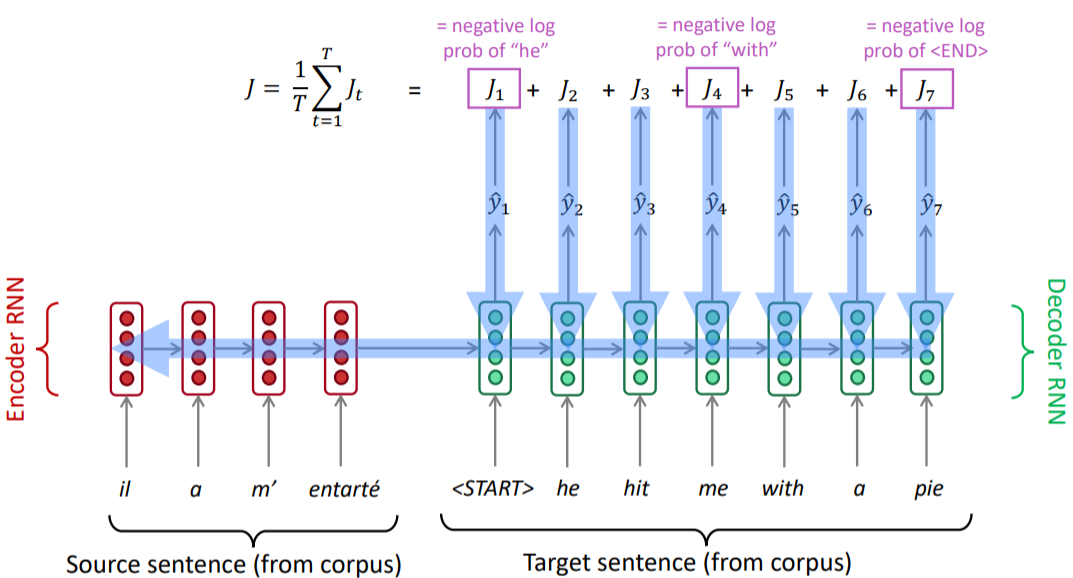
\includegraphics[width=8.0cm]{figs/NMT_training.png}}
	\caption{Training phase for NMT.}
	\label{fig:NMT_training}
\end{figure}

However, the aforementioned (greedy) decoding has no way to undo decisions. This is, if one of the output words are wrong, all the follow-up outputs are also wrong.
\concept{Beam search} decoding is utilized to fix this problem: on each step of decoder, keep track of the $k$ (in practice around $5$ to $10$) most probable partial translation (\emph{hypotheses}, path, or branch).
The target is the path with the largest cumulative log probabilities with shortest one (i.e. average).
Apart from all paths reach <END> as the stop sign, we can set some pre-defined cutoff for maximum number of timesteps or finished paths.

Although NMT is much simple and less human engineering effort while achieves better performance, NMT is diffcult to control (i.e. specify rules or guidelines) and less interpretable which leads to hard to debug.

The popular evaluation metric for MT is \concept{BLEU} (Bilingual Evaluation Understudy).
Its calculation is based on n-gram precision plus a penality for too-short translations.
Note that BLEU is useful but imperfect because there are many valid translations which has low $n$-gram overlap with the ground truth translation.
NMT outperforms SMT quickly, but there are still many difficulties remain:
\begin{itemize}
	\item Out-of-vocabulary words.
	\item Domain mismatch between train and test data.
	\item Maintaining context over longer text (long-term dependencies).
	\item Low-resource language pairs (few-shot learning).
	\item Using common sense is still hard.
\end{itemize}

\begin{figure}[!thp]
	\centerline{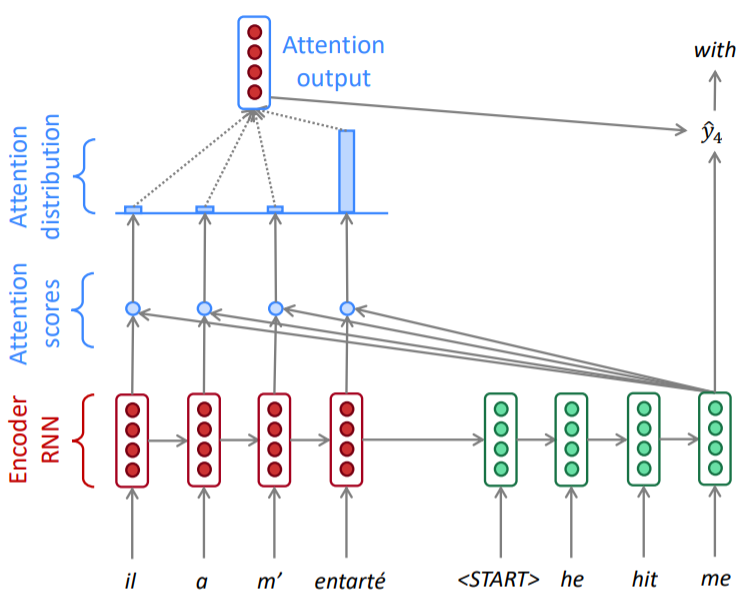
\includegraphics[width=8.0cm]{figs/Seq2Seq_attention.png}}
	\caption{Seq2Seq with attention.}
	\label{fig:Seq2Seq_Attention}
\end{figure}

We notice that only the last hidden state from encoder RNN to represent the whole source sentence may be the information bottleneck.
Thus we introduce Seq2Seq with \concept{attention}: on each step of the decoder, we use the attention distribution (like soft version of alignment) for each hidden states of encoder RNN to take a weighted sum of the encoder hidden states as the current decoder hidden state.
Note that sometimes the input of decoder RNN will concatenate the previous translated word vector and the previous attention output.
The diagram can be seen in Fig.\ref{fig:Seq2Seq_Attention}.
In addition, attention in here helps with vanishing gradient problem by providing shortcut to faraway states, and also provides some interpretability.
More formally, the attention for Seq2Seq is:
\begin{align}
&\bm{e}^{(t)} = [\bm{s}_t^\top \bm{h}_1, \cdots, \bm{s}_t^\top \bm{h}_n] \in \mathbb{R}^n \nonumber \\
&\text{Attention distribution: } \bm{\alpha}^{(t)} = \texttt{softmax}(\bm{e}^{(t)}) \nonumber \\
&\text{Attention ouput: } \bm{a}^{(t)} = \sum_{i=1}^n \alpha_i^t \bm{h}_i \in \mathbb{R}^h \nonumber \\
&\text{Attention decoder hidden state: } [\bm{a}^{(t)}; \bm{s}_t] \in \mathbb{R}^{2h}
\end{align}
where encoder hidden states $\bm{h}_1, \cdots, \bm{h}_n \in \mathbb{R}^h$, and decoder hidden state at timestep $t$ is $\bm{s}_t \in \mathbb{R}^h$.

More general definition of attention: given a set of vector \emph{values}, and a vector \emph{query}, attention is to compute a weighted sum of the values, dependent on the query.
We can found that attention is a way to obtain a \emph{fixed-size} representation of an arbitrary set of representations (e.g. sequential features).
There are many ways to obtain query vector: dot product $e_i = \bm{s}^\top \bm{h}_i$, multiplicative $e_i = \bm{s}^\top \bm{W} \bm{h}_i$, additive $e_i = \bm{v}^\top \tanh (\bm{W}_1 \bm{h}_i + \bm{W}_2 \bm{s})$, where $\bm{v}, \bm{W}, \bm{W}_1, \bm{W}_2$ are trainable parameters.

\section{Contextual Word Representations and Pretraining} \label{contextual_word_rep}
%\chapter{Decision Trees} \label{sec:dt}

\chapterquote{The words printed here are concepts.\\You must go through the experiences.}{Carl~Frederick}


%\chapterimageopt{serious.png}{width=5cm}{Courtesy XKCD}

\begin{learningobjectives}
\item Explain the difference between memorization and generalization.
\item Implement a decision tree classifier.
\item Take a concrete task and cast it as a learning problem, with a
  formal notion of input space, features, output space, generating
  distribution and loss function.
\end{learningobjectives}

\dependencies{None.}

At a basic level, machine learning is about predicting
the future based on the past.  For instance, you might wish to predict
how much a user Alice will like a movie that she hasn't seen, based on
her ratings of movies that she has seen. This prediction could be based
on many factors of the movies: their category (drama, documentary, etc.),
the language, the director and actors, the production company, etc.
In general, this means making informed
guesses about some unobserved property of some object, based on
observed properties of that object.

The first question we'll ask is: what does it mean to learn?  In order
to develop learning machines, we must know what learning actually
means, and how to determine success (or failure).  You'll see this
question answered in a very limited learning setting, which will be
progressively loosened and adapted throughout the rest of this book.
For concreteness, our focus will be on a very simple model of learning
called a \concept{decision tree}.

\section{What Does it Mean to Learn?}

Alice has just begun taking a course on machine learning.  She knows
that at the end of the course, she will be expected to have ``learned''
all about this topic.  A common way of gauging whether or not she has
learned is for her teacher, Bob, to give her a exam.  She has done
well at learning if she does well on the exam.

But what makes a reasonable exam?  If Bob spends the entire semester
talking about machine learning, and then gives Alice an exam on
History of Pottery, then Alice's performance on this exam will
\emph{not} be representative of her learning.  On the other hand, if
the exam only asks questions that Bob has answered exactly during lectures,
then this is also a bad test of Alice's learning, especially if it's
an ``open notes'' exam.  What is desired is that Alice observes
\emph{specific} examples from the course, and then has to answer new, but
related questions on the exam.  This tests whether Alice has the
ability to \concept{generalize}.  Generalization is perhaps the most
central concept in machine learning.

As a concrete example, consider a
course recommendation system for undergraduate computer science
students.  We have a collection of students and a collection of
courses.  Each student has taken, and evaluated, a subset of the
courses.  The evaluation is simply a score from $-2$ (terrible) to
$+2$ (awesome).  The job of the recommender system is to
\concept{predict} how much a particular student (say, Alice) will like
a particular course (say, Algorithms).

Given historical data from course ratings (i.e., the past) we are
trying to predict unseen ratings (i.e., the future).  Now, we could be
unfair to this system as well.  We could ask it whether Alice is
likely to enjoy the History of Pottery course.  This is unfair because
the system has no idea what History of Pottery even is, and has no
prior experience with this course.  On the other hand, we could ask it
how much Alice will like Artificial Intelligence, which she took last
year and rated as $+2$ (awesome).  We would expect the system to
predict that she would really like it, but this isn't demonstrating
that the system has learned: it's simply recalling its past
experience.  In the former case, we're expecting the system to
generalize \emph{beyond} its experience, which is unfair.  In the
latter case, we're not expecting it to generalize at all.

This general set up of predicting the future based on the past is at
the core of most machine learning.  The objects that our algorithm
will make predictions about are \concept{examples}.  In the
recommender system setting, an example would be some particular
Student/Course pair (such as Alice/Algorithms).  The desired
prediction would be the rating that Alice would give to Algorithms.

\Figure{dt_induction}{The general supervised approach to machine
  learning: a learning algorithm reads in training data and computes a
  learned function $f$.  This function can then automatically label
  future text examples.}

To make this concrete, Figure~\ref{fig:dt_induction} shows the general
framework of \concept{induction}.  We are given \concept{training
  data} on which our algorithm is expected to learn.  This training
data is the examples that Alice observes in her machine learning
course, or the historical ratings data for the recommender system.
Based on this training data, our learning algorithm induces a function
$f$ that will map a new example to a corresponding prediction.  For
example, our function might guess that $f(\text{Alice/Machine
  Learning})$ might be high because our training data said that Alice
liked Artificial Intelligence.  We want our algorithm to be able to
make lots of predictions, so we refer to the collection of examples on
which we will evaluate our algorithm as the \concept{test set}.  The
test set is a closely guarded secret: it is the final exam on which
our learning algorithm is being tested.  If our algorithm gets to peek
at it ahead of time, it's going to cheat and do better than it should.

\thinkaboutit{Why is it bad if the learning algorithm gets to peek at the test data?}

The goal of inductive machine learning is to take some training data
and use it to induce a function $f$.  This function $f$ will be
evaluated on the test data.  The machine learning algorithm has
succeeded if its performance on the test data is high.

\section{Some Canonical Learning Problems}

There are a large number of typical inductive learning problems.  The
primary difference between them is in what type of \emph{thing}
they're trying to predict.  Here are some examples:

\begin{description}
\item[Regression:] trying to predict a real value.  For instance,
  predict the value of a stock tomorrow given its past performance.
  Or predict Alice's score on the machine learning final exam based on
  her homework scores.

\item[Binary Classification:] trying to predict a simple yes/no
  response.  For instance, predict whether Alice will enjoy a course
  or not.  Or predict whether a user review of the newest Apple
  product is positive or negative about the product.

\item[Multiclass Classification:] trying to put an example into one of
  a number of classes.  For instance, predict whether a news story is
  about entertainment, sports, politics, religion, etc.  Or predict
  whether a CS course is Systems, Theory, AI or Other.

\item[Ranking:] trying to put a set of objects in order of relevance.
  For instance, predicting what order to put web pages in, in response
  to a user query.  Or predict Alice's ranked preferences over courses
  she hasn't taken.
\end{description}

\thinkaboutit{For each of these types of canonical machine learning
  problems, come up with one or two concrete examples.}

The reason that it is convenient to break machine learning problems
down by the type of object that they're trying to predict has to do
with measuring error.  Recall that our goal is to build a system that
can make ``good predictions.''  This begs the question: what does it
mean for a prediction to be ``good?''  The different types of learning
problems differ in how they define goodness.  For instance, in
regression, predicting a stock price that is off by $\$0.05$ is
perhaps much better than being off by $\$200.00$.  The same does not
hold of multiclass classification.  There, accidentally predicting
``entertainment'' instead of ``sports'' is no better or worse than
predicting ``politics.''


\section{The Decision Tree Model of Learning}

The \concept{decision tree} is a classic and natural model of
learning.  It is closely related to the fundamental computer science
notion of ``divide and conquer.''  Although decision trees can be
applied to many learning problems, we will begin with the simplest
case: binary classification.

Suppose that your goal is to predict whether some unknown user will
enjoy some unknown course.  You must simply answer ``yes'' or ``no.''
In order to make a guess, you're allowed to ask binary questions
about the user/course under consideration.  For example:

{\bf You:} Is the course under consideration in Systems?\\
{\bf Me:}  Yes\\
{\bf You:} Has this student taken any other Systems courses?\\
{\bf Me:}  Yes\\
{\bf You:} Has this student liked most previous Systems courses?\\
{\bf Me:}  No\\
{\bf You:} \emph{I predict this student will not like this course.}\\

The goal in learning is to figure out what questions to ask, in what
order to ask them, and what answer to predict once you have asked
enough questions.

\MoveNextFigure{-10cm}
\Figure{dt_example}{A decision tree for a course recommender system,
  from which the in-text ``dialog'' is drawn.}

The decision tree is so-called because we can write our set of
questions and guesses in a tree format, such as that in
Figure~\ref{fig:dt_example}.  In this figure, the questions are
written in the internal tree nodes (rectangles) and the guesses are
written in the leaves (ovals).  Each non-terminal node has two
children: the left child specifies what to do if the answer to the
question is ``no'' and the right child specifies what to do if it is
``yes.''

In order to learn, I will give you training data.  This data consists
of a set of user/course examples, paired with the correct answer for
these examples (did the given user enjoy the given course?).  From
this, you must construct your questions.  For concreteness, there is a
small data set in Table~\ref{tab:data:course} in the Appendix of this
book.  This training data consists of 20 course rating examples, with
course ratings and answers to questions that you might ask about this
pair.  We will interpret ratings of $0$, $+1$ and $+2$ as ``liked'' and
ratings of $-2$ and $-1$ as ``hated.''

In what follows, we will refer to the questions that you can ask as
\concept{features} and the responses to these questions as
\concept{feature values}.  The rating is called the \concept{label}.
An example is just a set of feature values.  And our training data is
a set of examples, paired with labels.

There are a lot of logically possible trees that you could build, even
over just this small number of features (the number is in the
millions).  It is computationally infeasible to consider all of these
to try to choose the ``best'' one.  Instead, we will build our
decision tree \emph{greedily.}  We will begin by asking:

{\bf If I could only ask one question, what question would I ask?}


\MoveNextFigure{-10cm}
\Figure{dt_histogram}{A histogram of labels for (a) the entire data
  set; (b-e) the examples in the data set for each value of the first
  four features.}

You want to find a feature that is \emph{most useful} in helping you
guess whether this student will enjoy this course.
A useful way to think about this is to look at the \concept{histogram}
of labels for each feature.  
\sidenote{A
  colleague related the story of getting his 8-year old nephew to
  guess a number between 1 and 100.  His nephew's first four questions
  were: Is it bigger than 20?  (YES) Is it even?  (YES) Does it have a
  7 in it?  (NO) Is it 80?  (NO).  It took 20 more questions to get
  it, even though 10 should have been sufficient.  At 8, the nephew
  hadn't quite figured out how to divide and conquer.
\url{http://blog.computationalcomplexity.org/2007/04/getting-8-year-old-interested-in.html}.}
This is shown for the first four features
in Figure~\ref{fig:dt_histogram}.  Each histogram shows the frequency
of ``like''/``hate'' labels for each possible value of an associated
feature.  From this figure, you can see that asking the first feature
is not useful: if the value is ``no'' then it's hard to guess the
label; similarly if the answer is ``yes.''  On the other hand, asking
the second feature \emph{is} useful: if the value is ``no,'' you can
be pretty confident that this student will hate this course; if the
answer is ``yes,'' you can be pretty confident that this student will
like this course.

More formally, you will consider each feature in turn.  You might
consider the feature ``Is this a System's course?''  This feature has
two possible value: no and yes.  Some of the training examples have an
answer of ``no'' -- let's call that the ``NO'' set.  Some of the
training examples have an answer of ``yes'' -- let's call that the
``YES'' set.  For each set (NO and YES) we will build a histogram over
the labels.  This is the second histogram in
Figure~\ref{fig:dt_histogram}.  Now, suppose you were to ask this
question on a random example and observe a value of ``no.''  Further
suppose that you must \emph{immediately} guess the label for this
example.  You will guess ``like,'' because that's the more prevalent
label in the NO set (actually, it's the \emph{only} label in the NO
set).  Alternatively, if you receive an answer of ``yes,'' you will
guess ``hate'' because that is more prevalent in the YES set.

So, for this single feature, you know what you \emph{would} guess if
you had to.  Now you can ask yourself: if I made that guess on the
\emph{training data,} how well would I have done?  In particular, how
many examples would I classify \emph{correctly?}  In the NO set (where
you guessed ``like'') you would classify all $10$ of them correctly.
In the YES set (where you guessed ``hate'') you would classify $8$
(out of $10$) of them correctly.  So overall you would classify $18$
(out of $20$) correctly.  Thus, we'll say that the \emph{score} of the
``Is this a System's course?'' question is $18/20$.

\thinkaboutit{How many training examples would you classify correctly
  for each of the other three features from
  Figure~\ref{fig:dt_histogram}?}

You will then repeat this computation for each of the available
features to us, compute the scores for each of them.  When you must
choose which feature consider first, you will want to choose the one
with the highest score.

But this only lets you choose the \emph{first} feature to ask about.
This is the feature that goes at the \emph{root} of the decision tree.
How do we choose subsequent features?  This is where the notion of
divide and conquer comes in.  You've already decided on your first
feature: ``Is this a Systems course?''  You can now \emph{partition}
the data into two parts: the NO part and the YES part.  The NO part is
the subset of the data on which value for this feature is ``no''; the
YES half is the rest.  This is the \emph{divide} step.

The \emph{conquer} step is to recurse, and run the \emph{same}
routine (choosing the feature with the highest score) on the NO set
(to get the left half of the tree) and then separately on the YES set
(to get the right half of the tree).

At some point it will become useless to query on additional features.
For instance, once you know that this is a Systems course, you
\emph{know} that everyone will hate it.  So you can immediately
predict ``hate'' without asking any additional questions.  Similarly,
at some point you might have already queried every available feature
and still not whittled down to a single answer.  In both cases, you
will need to create a leaf node and guess the most prevalent answer in
the current piece of the training data that you are looking at.


\newalgorithm%
  {dt:train}%
  {\FUN{DecisionTreeTrain}(\VAR{data}, \VAR{remaining features})}%
  {
\SETST{guess} most frequent answer in \VAR{data} \COMMENT{default answer for this data}
\IF{the labels in \VAR{data} are unambiguous}
\RETURN \STR{Leaf}(\VAR{guess}) \COMMENT{base case: no need to split further}
\ELSIF{\VAR{remaining features} is empty}
\RETURN \STR{Leaf}(\VAR{guess}) \COMMENT{base case: cannot split further}
\ELSE[we need to query more features]
\FORALL{\VAR{f} $\in$ \VAR{remaining features}}
\SETST{NO} the subset of \VAR{data} on which \VAR{f}=\CON{no}
\SETST{YES} the subset of \VAR{data} on which \VAR{f}=\CON{yes}
\STATE \VAR{score}[\VAR{f}] $\leftarrow$ \# of majority vote answers in \VAR{NO}
\STATE \quad\quad\quad\quad + \# of majority vote answers in \VAR{YES}\\
\COMMENT{the accuracy we would get if we only queried on \VAR{f}}
\ENDFOR
\SETST{f} the feature with maximal \VAR{score}(\VAR{f})
\SETST{NO} the subset of \VAR{data} on which \VAR{f}=\CON{no}
\SETST{YES} the subset of \VAR{data} on which \VAR{f}=\CON{yes}
\SETST{left} \FUN{DecisionTreeTrain}(\VAR{NO}, \VAR{remaining features} $\without$ $\{$\VAR{f}$\}$)
\SETST{right} \FUN{DecisionTreeTrain}(\VAR{YES}, \VAR{remaining features} $\without$ $\{$\VAR{f}$\}$)
\RETURN \STR{Node}(\VAR{f}, \VAR{left}, \VAR{right})
\ENDIF
}

\newalgorithm%
  {dt:predict}%
  {\FUN{DecisionTreeTest}(\VAR{tree}, \VAR{test point})}
  {
\IF{\VAR{tree} is of the form \STR{Leaf}(\VAR{guess})}
\RETURN \VAR{guess}
\ELSIF{\VAR{tree} is of the form \STR{Node}(\VAR{f}, \VAR{left}, \VAR{right})}
\IF{\VAR{f} $=$ \CON{no} in \VAR{test point}}
\RETURN \FUN{DecisionTreeTest}(\VAR{left}, \VAR{test point})
\ELSE
\RETURN \FUN{DecisionTreeTest}(\VAR{right}, \VAR{test point})
\ENDIF
\ENDIF
}

Putting this all together, we arrive at the algorithm shown in
Algorithm~\ref{alg:dt:train}.\sidenote{There are more nuanced
  algorithms for building decision trees, some of which are discussed
  in later chapters of this book.  They primarily differ in how they
  compute the \emph{score} function.}  This function,
\FUN{DecisionTreeTrain} takes two arguments: our data, and the set of
as-yet unused features.  It has two base cases: either the data is
unambiguous, or there are no remaining features.  In either case, it
returns a \STR{Leaf} node containing the most likely guess at this
point.  Otherwise, it loops over all remaining features to find the
one with the highest score.  It then partitions the data into a NO/YES
split based on the best feature.  It constructs its left and right
subtrees by recursing on itself.  In each recursive call, it uses one
of the partitions of the data, and removes the just-selected feature
from consideration.

\thinkaboutit{Is Algorithm~\ref{alg:dt:train}
  guaranteed to terminate?}

The corresponding \emph{prediction} algorithm is shown in
Algorithm~\ref{alg:dt:predict}.  This function recurses down the decision
tree, following the edges specified by the feature values in some
\VAR{test point}.  When it reaches a leaf, it returns the guess
associated with that leaf.

\section{Formalizing the Learning Problem}

As you've seen, there are several issues that we must take into
account when formalizing the notion of learning.

\begin{itemize}
\item The performance of the learning algorithm should be measured on
  unseen ``test'' data.

\item The way in which we measure performance should depend on the
  problem we are trying to solve.

\item There should be a strong relationship between the data that our
  algorithm sees at training time and the data it sees at test time.
\end{itemize}

In order to accomplish this, let's assume that someone gives us a
\concept{loss function}, $\ell(\cdot,\cdot)$, of two arguments.  The
job of $\ell$ is to tell us how ``bad'' a system's prediction is in
comparison to the truth.  In particular, if $y$ is the truth and $\hat
y$ is the system's prediction, then $\ell(y,\hat y)$ is a measure of
error.

For three of the canonical tasks discussed above, we might use the
following loss functions:

\begin{description}
\item[Regression:] \concept{squared loss} $\ell(y,\hat y) = (y - \hat
  y)^2$\\ or \concept{absolute loss} $\ell(y,\hat y) = \ab{y - \hat y}$.

\item[Binary Classification:] \concept{zero/one loss} $\ell(y,\hat y)
  = \brack{0 & \text{if } y = \hat y\\ 1 & \text{otherwise}}$
  \marginnote[-.5em]{This notation means that the loss is zero if the
    prediction is correct and is one otherwise.}

\item[Multiclass Classification:] also zero/one loss.
\end{description}

\thinkaboutit{Why might it be a bad idea to use zero/one loss to
  measure performance for a regression problem?}

Note that the loss function is something that \emph{you} must decide
on based on the goals of learning.

\begin{mathreview}{Expectated Values}
We write $\Ep_{(\vx,y) \sim \cD} [ \ell(y, f(\vx)) ]$ for the expected loss. Expectation means ``average.'' This is saying ``if you drew a bunch of $(x,y)$ pairs independently at random from $\cD$, what would your \emph{average} loss be?% (More formally, what would be the average of $\ell(y,f(\vx))$ be over these random draws?)
More formally, if $\cD$ is a discrete probability distribution, then this expectation can be expanded as:
%
\begin{equation}
  \Ep_{(\vx,y) \sim \cD} [ \ell(y, f(\vx)) ] = \sum_{(\vx,y) \in \cD} [ \cD(\vx,y) \ell(y, f(\vx)) ]
\end{equation}
%
This is \emph{exactly} the weighted average loss over the all $(\vx,y)$ pairs in $\cD$, weighted by their probability, $\cD(\vx,y)$.
If $D$ is a \emph{finite discrete distribution}, for instance defined by a finite data set $\{ (\vx_1,y_1), \dots, (\vx_N,y_N)$ that puts equal weight on each example (probability $1/N$), then we get:
%
\begin{align}
\Ep_{(\vx,y) \sim D} [ \ell(y, f(\vx)) ] 
&= \sum_{(\vx,y) \in D} [ D(\vx,y) \ell(y, f(\vx)) ]
   \becauseof{definition of expectation}\\
&= \sum_{n=1}^N [ D(\vx_n,y_n) \ell(y_n, f(\vx_n)) ]
   \becauseof{$D$ is discrete and finite}\\
&= \sum_{n=1}^N [ \frac 1 N \ell(y_n, f(\vx_n)) ] 
   \becauseof{definition of $D$}\\
&= \frac 1 N  \sum_{n=1}^N [ \ell(y_n, f(\vx_n)) ]
   \becauseof{rearranging terms}
\end{align}
%
Which is exactly the average loss on that dataset.
\\~\\
%In the case that the distribution is continuous, we need to replace the discrete sum with a continuous integral over some space $\Omega$:
%$  \Ep_{(\vx,y) \sim \cD} [ \ell(y, f(\vx)) ] = \int_{\Omega} \cD(\vx,y) \ell(y, f(\vx)) \ud \vx \ud y
%$.
%This is exactly the same but in continuous space rather than discrete space.
The most important thing to remember is that there are two equivalent ways to think about expections:
(1) The expectation of some function $g$ is the \emph{weighted average value of $g$}, where the weights are given by the underlying probability distribution.
(2) The expectation of some function $g$ is your \emph{best guess of the value of $g$} if you were to draw a single item from the underlying probability distribution.
\end{mathreview}

Now that we have defined our loss function, we need to consider where
the data (training \emph{and} test) comes from.  The model that we
will use is the \emph{probabilistic} model of learning.  Namely, there
is a probability distribution $\cD$ over input/output pairs.  This is
often called the \concept{data generating distribution}.  If we write
$\vx$ for the input (the user/course pair) and $y$ for the output (the
rating), then $\cD$ is a distribution over $(\vx,y)$ pairs.

A useful way to think about $\cD$ is that it gives \emph{high
  probability} to reasonable $(\vx,y)$ pairs, and \emph{low
  probability} to unreasonable $(\vx,y)$ pairs.  A $(\vx,y)$ pair can
be unreasonable in two ways.  First, $\vx$ might be an unusual input.
For example, a $\vx$ related to an ``Intro to Java'' course might be
highly probable; a $\vx$ related to a ``Geometric and Solid Modeling''
course might be less probable.  Second, $y$ might be an unusual rating
for the paired $\vx$.  For instance, if Alice were to take AI $100$
times (without remembering that she took it before!), she would give
the course a $+2$ almost every time.  Perhaps some semesters she might
give a slightly lower score, but it would be unlikely to see
$\vx=$Alice/AI paired with $y=-2$.

It is important to remember that we are not making \emph{any}
assumptions about what the distribution $\cD$ looks like.  (For
instance, we're not assuming it looks like a Gaussian or some other,
common distribution.)  We are also not assuming that we know what
$\cD$ is.  In fact, if you know \emph{a priori} what your data
generating distribution is, your learning problem becomes
significantly easier.  Perhaps the hardest thing about machine
learning is that we \emph{don't} know what $\cD$ is: all we get is a
random sample from it.  This random sample is our training data.

Our learning problem, then, is defined by two quantities:

\thinkaboutit{Consider the following prediction task.  Given a
  paragraph written about a course, we have to predict whether the
  paragraph is a \emph{positive} or \emph{negative} review of the
  course.  (This is the sentiment analysis problem.)  What is a
  reasonable loss function?  How would you define the data generating
  distribution?}
\begin{enumerate}
\item The loss function $\ell$, which captures our notion of what is
  \emph{important} to learn.

\item The data generating distribution $\cD$, which defines what sort
  of data we expect to see.
\end{enumerate}

We are given access to \concept{training data}, which is a random
sample of input/output pairs drawn from $\cD$.  Based on this training
data, we need to \concept{induce} a function $f$ that maps new inputs
$\hat \vx$ to corresponding prediction $\hat y$.  The key property
that $f$ should obey is that it should do well (as measured by $\ell$)
on future examples that are \emph{also} drawn from $\cD$.  Formally,
it's \concept{expected loss} $\ep$ over $\cD$ with repsect to $\ell$
should be as small as possible:
\begin{align} \label{eq:expectederror}
\ep
&\defeq
\Ep_{(\vx,y) \sim \cD} \big[ \ell(y, f(\vx)) \big]
=
\sum_{(\vx,y)} \cD(\vx,y) \ell(y, f(\vx))
\end{align}

The difficulty in minimizing our \concept{expected loss} from
Eq~\eqref{eq:expectederror} is that we \emph{don't know what $\cD$
  is!}  All we have access to is some training data sampled from it!
Suppose that we denote our training data set by $D$.  The training
data consists of $N$-many input/output pairs, $(\vx_1,y_1),
(\vx_2,y_2), \dots, (\vx_N,y_N)$.  Given a learned function $f$, we
can compute our \concept{training error}, $\hat \ep$:
\begin{align} \label{eq:trainingerror}
\hat \ep
&\defeq
\frac 1 N \sum_{n=1}^N \ell(y_n, f(\vx_n))
\end{align}

That is, our training error is simply our \emph{average error} over
the training data.  \thinkaboutit{Verify by calculation that we can
  write our training error as $\Ep_{(\vx,y) \sim D} \big[ \ell(y,
  f(\vx)) \big]$, by thinking of $D$ as a distribution that places
  probability $1/N$ to each example in $D$ and probability $0$ on
  everything else.}

Of course, we can drive $\hat \ep$ to zero by simply memorizing our
training data.  But as Alice might find in memorizing past exams, this
might not generalize well to a new exam!

This is the fundamental difficulty in machine learning: the thing we
have access to is our training error, $\hat \ep$.  But the thing we care
about minimizing is our expected error $\ep$.  In order to get the
expected error down, our learned function needs to
\concept{generalize} beyond the training data to some future data that
it might not have seen yet!

So, putting it all together, we get a formal definition of induction
machine learning: \bigemph{Given (i) a loss function $\ell$ and (ii) a
  sample $D$ from some unknown distribution $\cD$, you must compute a
  function $f$ that has low expected error $\ep$ over $\cD$ with
  respect to $\ell$.}

A very important comment is that we should \emph{never} expect a machine learning algorithm to generalize beyond the data distribution it has seen at training time.
In a famous---if posssibly apocryphal---example from the 1970s, the US Government wanted to train a classifier to distinguish between US tanks and Russian tanks.
They collected a training and test set, and managed to build a classifier with nearly 100\% accuracy on that data.
But when this classifier was run in the ``real world'', it failed miserably.
It had not, in fact, learned to distinguish between US tanks and Russian tanks, but rather just between clear photos and blurry photos.
In this case, there was a \emph{bias} in the training data (due to how the training data was collected) that caused the learning algorithm to learn something other than what we were hoping for.
We will return to this issue in Chapter~\ref{sec:bias}; for now, simply remember that the distribution $D$ for training data \emph{must match} the distribution $D$ for the test data.



\section{Chapter Summary and Outlook}

At this point, you should be able to use decision trees to do machine
learning.  Someone will give you data.  You'll split it into
training, development and test portions.  Using the training and
development data, you'll find a good value for maximum depth that
trades off between underfitting and overfitting.  You'll then run the
resulting decision tree model on the test data to get an estimate of
how well you are likely to do in the future.

You might think: why should I read the rest of this book?  Aside from
the fact that machine learning is just an awesome fun field to learn
about, there's a lot left to cover.  In the next two chapters, you'll
learn about two models that have very different inductive biases than
decision trees.  You'll also get to see a very useful way of thinking
about learning: the geometric view of data.  This will guide much of
what follows.  After that, you'll learn how to solve problems more
complicated that simple binary classification.  (Machine learning
people like binary classification a lot because it's one of the
simplest non-trivial problems that we can work on.)  After that,
things will diverge: you'll learn about ways to think about learning
as a formal optimization problem, ways to speed up learning, ways to
learn without labeled data (or with very little labeled data) and all
sorts of other fun topics.

But throughout, we will focus on the view of machine learning that
you've seen here.  You select a model (and its associated inductive
biases).  You use data to find parameters of that model that work well
on the training data.  You use development data to avoid underfitting
and overfitting.  And you use test data (which you'll never look at or
touch, right?) to estimate future model performance.  Then you conquer
the world.

%\section{Decision Trees with Real-Valued Features}


\section{Further Reading}

In our discussion of decision trees, we used \emph{misclassification rate} for selecting features.
While simple and intuitive, misclassification rate has problems.
There has been a significant amount of work that considers more advanced splitting criteria; the most popular is ID3, based on the mutual information quantity from information theory.
We have also only considered a very simple mechanism for controlling inductive bias: limiting the depth of the decision tree.
Again, there are more advanced ``tree pruning'' techniques that typically operate by growing deep trees and then pruning back some of the branches.
These approaches have the advantage that different branches can have different depths, accounting for the fact that the amount of data that gets passed down each branch might differ dramatically\mycite{quinlan}.


\begin{comment}
Predicting the future
 - Not memorizing the past (simple prediction problem)
 - Generalizing from known to unknown
 - Training versus test data

Models, algorithms, theory and experiments

Evaluation

Optimizing 0/1 loss

Underfitting/overfitting by depth

Pruning

From two classes to M classes
\end{comment}


%%% Local Variables: 
%%% mode: latex
%%% TeX-master: "courseml"
%%% End: 

%\chapter{Limits of Learning} \label{sec:formal}

\chapterquote{Our lives sometimes depend on computers performing as predicted.}{Philip~Emeagwali}


%\chapterimageopt{serious.png}{width=5cm}{Courtesy XKCD}

\begin{learningobjectives}
\item Define ``inductive bias'' and recognize the role of inductive
  bias in learning.
\item Illustrate how regularization trades off between underfitting
  and overfitting.
\item Evaluate whether a use of test data is ``cheating'' or not.
\end{learningobjectives}

\dependencies{None.}

\newthought{Machine learning is a very general} and useful framework, but it is not ``magic'' and will not always work.
In order to better understand when it will and when it will not work, it is useful to formalize the learning problem more.
This will also help us develop debugging strategies for learning algorithms.

\section{Data Generating Distributions}

Our underlying assumption for the majority of this book is that
learning problems are characterized by some unknown probability
distribution $\cD$ over input/output pairs $(x,y) \in \cX \times \cY$.
Suppose that someone \emph{told} you what $\cD$ was.  In particular,
they gave you a Python function \FUN{computeD} that took two inputs,
$x$ and $y$, and returned the probability of that $x,y$ pair under
$\cD$.  If you had access to such a function, classification becomes
simple.  We can define the \concept{Bayes optimal classifier} as the
classifier that, for any test input $\hat x$, simply returns the $\hat
y$ that maximizes \FUN{computeD}$(\hat x, \hat y)$, or, more formally:
%
\begin{equation} \label{eq:prob:bayesopt}
  f\xth{BO}(\hat x) = \arg\max_{\hat y \in \cY} \cD(\hat x, \hat y)
\end{equation}
%
This classifier is optimal in one specific sense: of \emph{all
  possible} classifiers, it achieves the smallest zero/one error.

\begin{theorem}[Bayes Optimal Classifier] \label{thm:prob:bayesopt}
  The Bayes Optimal Classifier $f\xth{BO}$ achieves minimal zero/one
  error of any deterministic classifier.
\end{theorem}

This theorem assumes that you are comparing against
\emph{deterministic} classifiers.  You can actually prove a stronger
result that $f\xth{BO}$ is optimal for randomized classifiers as well,
but the proof is a bit messier.  However, the intuition is the same:
for a given $x$, $f\xth{BO}$ chooses the label with highest
probability, thus \emph{minimizing} the probability that it makes an
error.

\begin{myproof}{\ref{thm:prob:bayesopt}}
  Consider some other classifier $g$ that claims to be better than
  $f\xth{BO}$.  Then, there must be some $x$ on which $g(x) \neq f\xth{BO}(x)$.  Fix
  such an $x$.  Now, the probability that $f\xth{BO}$ makes an error on this
  particular $x$ is $1 - \cD(x, f\xth{BO}(x))$ and the probability
  that $g$ makes an error on this $x$ is $1 - \cD(x, g(x))$.  But
  $f\xth{BO}$ was chosen in such a way to \emph{maximize} $\cD(x,
  f\xth{BO}(x))$, so this \emph{must} be greater than $\cD(x, g(x))$.
  Thus, the probability that $f\xth{BO}$ errs on this particular $x$ is
  smaller than the probability that $g$ errs on it.  This applies to
  any $x$ for which $f\xth{BO}(x) \neq g(x)$ and therefore $f\xth{BO}$ achieves
  smaller zero/one error than any $g$.
\end{myproof}

The \concept{Bayes error rate} (or \concept{Bayes optimal error rate})
is the error rate of the Bayes optimal classifier.  It is the best
error rate you can ever hope to achieve on this classification problem
(under zero/one loss).
%
The take-home message is that if someone gave you access to the data
distribution, forming an \emph{optimal} classifier would be trivial.
Unfortunately, no one gave you this distribution, so we need to 
figure out ways of learning the mapping from $x$ to $y$ given only access to a training set \emph{sampled from} $\cD$, rather than $\cD$ itself.

% Unfortunately, no one gave you this distribution, but this analysis
% suggests that good way to build a classifier is to try to
% \emph{estimate} $\cD$.  In other words, you try to learn a
% distribution $\hat \cD$, which you hope to very similar to $\cD$, and
% then use this distribution for classification.  Just as in the
% preceding chapters, you can try to form your estimate of $\cD$ based
% on a finite training set.

% The most direct way that you can attempt to construct such a
% probability distribution is to select a \emph{family} of parametric
% distributions.  For instance, a Gaussian (or Normal) distribution is
% parametric: it's parameters are its mean and covariance.  The job of
% learning is then to infer which parameters are ``best'' as far as the
% observed training data is concerned, as well as whatever inductive
% bias you bring.  A key assumption that you will need to make is that
% the training data you have access to is drawn \concept{independently}
% from $\cD$.  In particular, as you draw examples $(x_1,y_1) \sim \cD$
% then $(x_2,y_2) \sim \cD$ and so on, the $n$th draw $(x_n,y_n)$ is
% drawn from $\cD$ and \emph{does not} otherwise depend on the previous
% $n-1$ samples.  This assumption is usually false, but is also usually
% sufficiently close to being true to be useful.  Together with the
% assumption that all the training data is drawn from the same
% distribution $\cD$ leads to the \concept{i.i.d. assumption} or
% \concept{independently and identically distributed} assumption.  This
% is a key assumption in almost all of machine learning.


\section{Inductive Bias: What We Know Before the Data Arrives}

\Figure{dt_birdtrain}{Training data for a binary classification problem.}

\Figure{dt_birdtest}{Test data for the same classification problem.}

In Figure~\ref{fig:dt_birdtrain} you'll find training data for a binary
classification problem.  The two labels are ``A'' and ``B'' and you
can see four examples for each label.  Below, in
Figure~\ref{fig:dt_birdtest}, you will see some test data.  These
images are left unlabeled.  Go through quickly and, based on the
training data, label these images.  (Really do it before you read
further!  I'll wait!)

Most likely you produced one of two labelings: either ABBA or AABB. Which of these solutions is right?
The answer is that you cannot tell based on the training data.  If you
give this same example to $100$ people, $60-70$ of them come up with
the ABBA prediction and $30-40$ come up with the AABB prediction.
Why?  Presumably because the first group believes
that the relevant distinction is between ``bird'' and ``non-bird''
while the second group believes that the relevant distinction is
between ``fly'' and ``no-fly.''

This preference for one distinction (bird/non-bird) over another
(fly/no-fly) is a bias that different human learners have.  In the
context of machine learning, it is called \concept{inductive bias}: in
the absense of data that narrow down the relevant concept, what type
of solutions are we more likely to prefer?  Two thirds of people seem
to have an inductive bias in favor of bird/non-bird, and one third
seem to have an inductive bias in favor of fly/no-fly.

\thinkaboutit{It is also possible that the correct classification on
  the test data is ABAB.  This corresponds to the bias ``is the
  background in focus.''  Somehow no one seems to come up with this
  classification rule.}

Throughout this book you will learn about several approaches to
machine learning.  The decision tree model is the first such
approach.  These approaches differ primarily in the sort of inductive
bias that they exhibit.

Consider a variant of the decision tree learning algorithm.  In this
variant, we will not allow the trees to grow beyond some pre-defined
maximum depth, $d$.  That is, once we have queried on $d$-many
features, we cannot query on any more and must just make the best
guess we can at that point.  This variant is called a \concept{shallow
  decision tree}.

The key question is: What is the inductive bias of shallow decision
trees?  Roughly, their bias is that decisions can be made by only
looking at a small number of features.  For instance, a shallow
decision tree would be very good at learning a function like
``students only like AI courses.''  It would be very bad at learning a
function like ``if this student has liked an odd number of their past
courses, they will like the next one; otherwise they will not.''  This
latter is the \concept{parity} function, which requires you to inspect
every feature to make a prediction.  The inductive bias of a decision
tree is that the sorts of things we want to learn to predict are more
like the first example and less like the second example.

\section{Not Everything is Learnable}

Although machine learning works well---perhaps astonishingly well---in
many cases, it is important to keep in mind that it is not magical.
There are many reasons why a machine learning algorithm might fail on
some learning task.

There could be \concept{noise} in the training data.  Noise can occur
both at the feature level and at the label level.  Some features might
correspond to measurements taken by sensors.  For instance, a robot
might use a laser range finder to compute its distance to a wall.
However, this sensor might fail and return an incorrect value.  In a
sentiment classification problem, someone might have a typo in their
review of a course.  These would lead to noise at the feature level.
There might also be noise at the label level.  A student might write a
scathingly negative review of a course, but then accidentally click
the wrong button for the course rating.

The features available for learning might simply be insufficient.  For
example, in a medical context, you might wish to diagnose whether a
patient has cancer or not.  You may be able to collect a large amount
of data about this patient, such as gene expressions, X-rays, family
histories, etc.  But, even knowing all of this information exactly, it
might still be impossible to judge for sure whether this patient has
cancer or not.  As a more contrived example, you might try to classify
course reviews as positive or negative.  But you may have erred when
downloading the data and only gotten the first five characters of each
review.  If you had the rest of the features you might be able to do
well.  But with this limited feature set, there's not much you can do.

Some examples may not have a single correct answer.  You might be
building a system for ``safe web search,'' which removes offensive web
pages from search results.  To build this system, you would collect a
set of web pages and ask people to classify them as ``offensive'' or
not.  However, what one person considers offensive might be completely
reasonable for another person.  It is common to consider this as a
form of label noise.  Nevertheless, since you, as the designer of the
learning system, have some control over this problem, it is sometimes
helpful to isolate it as a source of difficulty.

Finally, learning might fail because the inductive bias of the
learning algorithm is too far away from the concept that is being
learned.  In the bird/non-bird data, you might think that if you had
gotten a few more training examples, you might have been able to tell
whether this was intended to be a bird/non-bird classification or a
fly/no-fly classification.  However, no one I've talked to has ever
come up with the ``background is in focus'' classification.  Even with
many more training points, this is such an unusual distinction that it
may be hard for anyone to figure out it.  In this case, the inductive
bias of the learner is simply too misaligned with the target
classification to learn.

Note that the inductive bias source of error is fundamentally
different than the other three sources of error.  In the inductive
bias case, it is the \emph{particular} learning algorithm that you are
using that cannot cope with the data.  Maybe if you switched to a
different learning algorithm, you would be able to learn well.  For
instance, Neptunians might have evolved to care greatly about whether
backgrounds are in focus, and for them this would be an easy
classification to learn.  For the other three sources of error, it is
not an issue to do with the particular learning algorithm.  The error
is a fundamental part of the learning problem.

\section{Underfitting and Overfitting}

As with many problems, it is useful to think about the \emph{extreme
  cases} of learning algorithms.  In particular, the extreme cases of
decision trees.  In one extreme, the tree is ``empty'' and we do not
ask any questions at all.  We simply immediately make a prediction.  In
the other extreme, the tree is ``full.''  That is, every possible
question is asked along every branch.  In the full tree, there may be
leaves with no associated training data.  For these we must simply
choose arbitrarily whether to say ``yes'' or ``no.''

Consider the course recommendation data from
Table~\ref{tab:data:course}.  Suppose we were to build an ``empty''
decision tree on this data.  Such a decision tree will make the same
prediction regardless of its input, because it is not allowed to ask
any questions about its input.  Since there are more ``likes'' than
``hates'' in the training data ($12$ versus $8$), our empty decision
tree will simply always predict ``likes.''  The training error, $\hat
\ep$, is $8/20 = 40\%$.

On the other hand, we could build a ``full'' decision tree.  Since
each row in this data is unique, we can guarantee that any leaf in a
full decision tree will have either $0$ or $1$ examples assigned to it
($20$ of the leaves will have one example; the rest will have none).
For the leaves corresponding to training points, the full decision
tree will always make the correct prediction.  
Given this, the training error, $\hat \ep$, is $0/20 = 0\%$.

Of course our goal is \emph{not} to build a model that gets $0\%$
error on the training data.  This would be easy!  Our goal is a model
that will do well on \emph{future, unseen} data.  How well might we
expect these two models to do on future data?  The ``empty'' tree is
likely to do not much better and not much worse on future data.  We
might expect that it would continue to get around $40\%$ error.

Life is more complicated for the ``full'' decision tree.  Certainly if
it is given a test example that is identical to one of the training
examples, it will do the right thing (assuming no noise).  But for
everything else, it will only get about $50\%$ error.  This means that
even if every other test point happens to be identical to one of the
training points, it would only get about $25\%$ error.  In practice,
this is probably optimistic, and maybe only one in every $10$ examples
would match a training example, yielding a $35\%$ error.

\thinkaboutit{Convince yourself (either by proof or by simulation)
  that even in the case of imbalanced data -- for instance data that
  is on average $80\%$ positive and $20\%$ negative -- a predictor
  that guesses randomly (50/50 positive/negative) will get about
  $50\%$ error.}

So, in one case (empty tree) we've achieved about $40\%$ error and in
the other case (full tree) we've achieved $35\%$ error.  This is not
very promising!  One would hope to do better!  In fact, you might
notice that if you simply queried on a \emph{single} feature for this
data, you would be able to get very low training error, but wouldn't
be forced to ``guess'' randomly.

\thinkaboutit{Which feature is it, and what is it's training error?}

This example illustrates the key concepts of \concept{underfitting}
and \concept{overfitting}.  Underfitting is when you had the
opportunity to learn something but didn't.  A student who hasn't
studied much for an upcoming exam will be underfit to the exam, and
consequently will not do well.  This is also what the empty tree
does.  Overfitting is when you pay too much attention to
idiosyncracies of the training data, and aren't able to generalize
well.  Often this means that your model is fitting noise, rather than
whatever it is supposed to fit.  A student who memorizes answers to
past exam questions without understanding them has overfit the
training data.  Like the full tree, this student also will not do well
on the exam.  A model that is neither overfit nor underfit is the one
that is expected to do best in the future.

\section{Separation of Training and Test Data}

Suppose that, after graduating, you get a job working for a company
that provides personalized recommendations for pottery.  You go in and
implement new algorithms based on what you learned in your machine
learning class (you have learned the power of generalization!).  All
you need to do now is convince your boss that you have done a good job
and deserve a raise!

How can you convince your boss that your fancy learning algorithms are
really working?

Based on what we've talked about already with underfitting and
overfitting, it is not enough to just tell your boss what your
training error is.  Noise notwithstanding, it is easy to get a
training error of zero using a simple database query (or {\tt grep},
if you prefer).  Your boss will not fall for that.

\begin{mathreview}{Law of Large Numbers}
  Consider some random event, like spins of a roulette wheel, cars
  driving through an intersection, the outcome of an election, or
  pasta being appropriately \emph{al dente.} We often want to make a
  conclusion about the entire population (the pot of pasta) based on a
  much smaller sample (biting a couple pieces of pasta). The law of
  large numbers tells us that under mild conditions this is an okay
  thing to do.

  ~

  Formally, suppose that $v_1, v_2, \dots, v_N$ are random variables
  (e.g., $v_n$ measures if the $n$th spaghetti is \emph{al
    dente}). Assume that these random variables are \concept{independent}
  (i.e., $v_2$ and $v_3$ are uncorrelated---they weren't both taken
  from the same place in the pot) and \concept{identically distributed}
  (they were all drawn from the same population---pot---that we wish
  to measure). We can compute the sample average $\bar v = \frac 1 N
  \sum_{n=1}^N v_n$ and under the \concept{strong law of large numbers},
  you can prove that $\bar v \rightarrow \Ep[v]$ as $N \rightarrow
  \infty$. Namely, the empirical sample average approaches the
  population average as the number of samples goes do infinity.

  ~

  \textit{(Technical note: the notion of convergence here is \emph{almost sure} convergence. In particular, the formal result is that $\textrm{Pr}\left(\lim_{N\rightarrow\infty} \frac 1 N \sum_n v_n = \Ep[v]\right) = 1$. Or, in words, with probability one the sample average reaches the population average.)}
\end{mathreview}

The easiest approach is to \emph{set aside} some of your available
data as ``test data'' and use this to evaluate the performance of your
learning algorithm.  For instance, the pottery recommendation service
that you work for might have collected $1000$ examples of pottery
ratings.  You will select $800$ of these as \concept{training data}
and set aside the final $200$ as \concept{test data}.  You will run
your learning algorithms \emph{only} on the $800$ training points.
Only once you're done will you apply your learned model to the $200$
test points, and report your \concept{test error} on those $200$
points to your boss.

The hope in this process is that however well you do on the $200$ test
points will be indicative of how well you are likely to do in the
future.  This is analogous to estimating support for a presidential
candidate by asking a small (random!) sample of people for their
opinions.  Statistics (specifically, concentration bounds of which the
``Central limit theorem'' is a famous example) tells us that if the
sample is large enough, it will be a good representative.  The 80/20
split is not magic: it's simply fairly well established.  Occasionally
people use a 90/10 split instead, especially if they have a \emph{lot}
of data.

\thinkaboutit{If you have more data at your disposal, why might a
  90/10 split be preferable to an 80/20 split?}

The cardinal rule of machine learning is: never touch your test data.
Ever.  If that's not clear enough:

\noindent
\begin{tikzpicture}[transform shape, rotate=0]
  \node [draw=Red!5, fill=Red!20, very thick, rectangle, rounded corners, inner sep=5pt, inner ysep=5pt] (box) {
    \textcolor{red}{\textsf{\huge Never \emph{ever} touch your test data!}}
  };
\end{tikzpicture}

If there is only one thing you learn from this book, let it be that.
Do not look at your test data.  Even once.  Even a tiny peek.  Once
you do that, it is not test data any more.  Yes, perhaps your
algorithm hasn't seen it.  But you have.  And you are likely a better
learner than your learning algorithm.  Consciously or otherwise, you
might make decisions based on whatever you might have seen.  Once you
look at the test data, your model's performance on it is no longer
indicative of it's performance on future unseen data.  This is simply
because future data is unseen, but your ``test'' data no longer is.

\section{Models, Parameters and Hyperparameters}

The general approach to machine learning, which captures many existing
learning algorithms, is the \concept{modeling} approach.  The idea is
that we come up with some formal model of our data.  For instance, we
might model the classification decision of a student/course pair as a
decision tree.  The choice of using a \emph{tree} to represent this
model is \emph{our choice.}  We also could have used an arithmetic
circuit or a polynomial or some other function.  The model tells us
what sort of things we can learn, and also tells us what our inductive
bias is.

For most models, there will be associated parameters.  These are the
things that we use the data to decide on.  Parameters in a decision
tree include: the specific questions we asked, the order in which we
asked them, and the classification decisions at the leaves.  The job
of our decision tree learning algorithm \FUN{DecisionTreeTrain} is to take data
and figure out a good set of parameters.

Many learning algorithms will have additional knobs that you can
adjust.  In most cases, these knobs amount to tuning the inductive
bias of the algorithm.  In the case of the decision tree, an obvious
knob that one can tune is the \concept{maximum depth} of the decision
tree.  That is, we could modify the \FUN{DecisionTreeTrain} function so that it
\emph{stops} recursing once it reaches some pre-defined maximum depth.
By playing with this depth knob, we can adjust between underfitting
(the empty tree, depth$=0$) and overfitting (the full tree,
depth$=\infty$).

\thinkaboutit{Go back to the \FUN{DecisionTreeTrain} algorithm and modify it so
  that it takes a maximum depth parameter.  This should require adding
  two lines of code and modifying three others.}

Such a knob is called a \concept{hyperparameter}.  It is so called
because it is a parameter that controls other parameters of the model.
The exact definition of hyperparameter is hard to pin down: it's one
of those things that are easier to identify than define.  However, one
of the key identifiers for hyperparameters (and the main reason that
they cause consternation) is that they cannot be naively adjusted
using the training data.

In \FUN{DecisionTreeTrain}, as in most machine learning, the learning algorithm
is essentially trying to adjust the parameters of the model so as to
minimize training error.  This suggests an idea for choosing
hyperparameters: choose them so that they minimize training error.

What is wrong with this suggestion?  Suppose that you were to treat
``maximum depth'' as a hyperparameter and tried to tune it on your
training data.  To do this, maybe you simply build a collection of
decision trees, tree$_0$, tree$_1$, tree$_2$, $\dots$, tree$_{100}$,
where tree$_d$ is a tree of maximum depth $d$.  We then computed the
training error of each of these trees and chose the ``ideal'' maximum
depth as that which minimizes training error?  Which one would it
pick?

The answer is that it would pick $d=100$.  Or, in general, it would
pick $d$ as large as possible.  Why?  Because choosing a bigger $d$
will \emph{never hurt} on the training data.  By making $d$ larger,
you are simply encouraging overfitting.  But by evaluating on the
training data, overfitting actually looks like a good idea!

An alternative idea would be to tune the maximum depth on test data.
This is promising because test data peformance is what we really want
to optimize, so tuning this knob on the test data seems like a good
idea.  That is, it won't accidentally reward overfitting.  Of course,
it breaks our cardinal rule about test data: that you should never
touch your test data.  So that idea is immediately off the table.

However, our ``test data'' wasn't magic.  We simply took our $1000$
examples, called $800$ of them ``training'' data and called the other
$200$ ``test'' data.  So instead, let's do the following.  Let's take
our original $1000$ data points, and select $700$ of them as training
data.  From the remainder, take $100$ as \concept{development
  data}\sidenote{Some people call this ``\concept{validation data}''
  or ``\concept{held-out data}.''} and the remaining $200$ as test
data.  The job of the development data is to allow us to tune
hyperparameters.  The general approach is as follows:

\begin{enumerate}
\item Split your data into $70\%$ training data, $10\%$ development
  data and $20\%$ test data.

\item For each possible setting of your hyperparameters:

\begin{enumerate}
\item Train a model using that setting of hyperparameters on the
  training data.

\item Compute this model's error rate on the development data.
\end{enumerate}

\item From the above collection of models, choose the one that
  achieved the lowest error rate on development data.

\item Evaluate that model on the test data to estimate future test
  performance.
\end{enumerate}

\thinkaboutit{In step 3, you could either choose the model (trained on
  the $70\%$ training data) that did the best on the development data.
  Or you could choose the hyperparameter settings that did best and
  \emph{retrain} the model on the $80\%$ union of training and
  development data.  Is either of these options obviously better or
  worse?}


\section{Real World Applications of Machine Learning}

Figure~\ref{fig:formal_deployml} shows a typical sequence of decisions that must be made to deploy a machine learning approach in the real world. In the left column, you can see the generic decision being made. In the right column, an example of this decision for the particular case of advertising placement on a search engine we've built.

In this sequence, (1) we have some real world goal like increasing revenue for our search engine, and decide to try to increase revenue by (2) displaying better ads. We convert this task into a machine learning problem by (3) deciding to train a classifier to predict whether a user will click on an ad or not. In order to apply machine learning, we must collect some training data; in this case, (4) we collect data by logging user interactions with the current system. We must choose what to log; (5) we choose to log the ad being displayed, the query the user entered into our search engine, and binary value showing if they clicked or not.

{
  \definecolor{lightcyan}{rgb}{0.88,1,1}
  \definecolor{lightpink}{rgb}{1,0.88,1}
  \newcolumntype{y}{>{\columncolor{lightcyan}}m{2cm}}
  \newcolumntype{z}{>{\columncolor{lightpink}}m{2cm}}
  \begin{marginfigure}[\NextFigureOffset]
    \begin{centering}
      %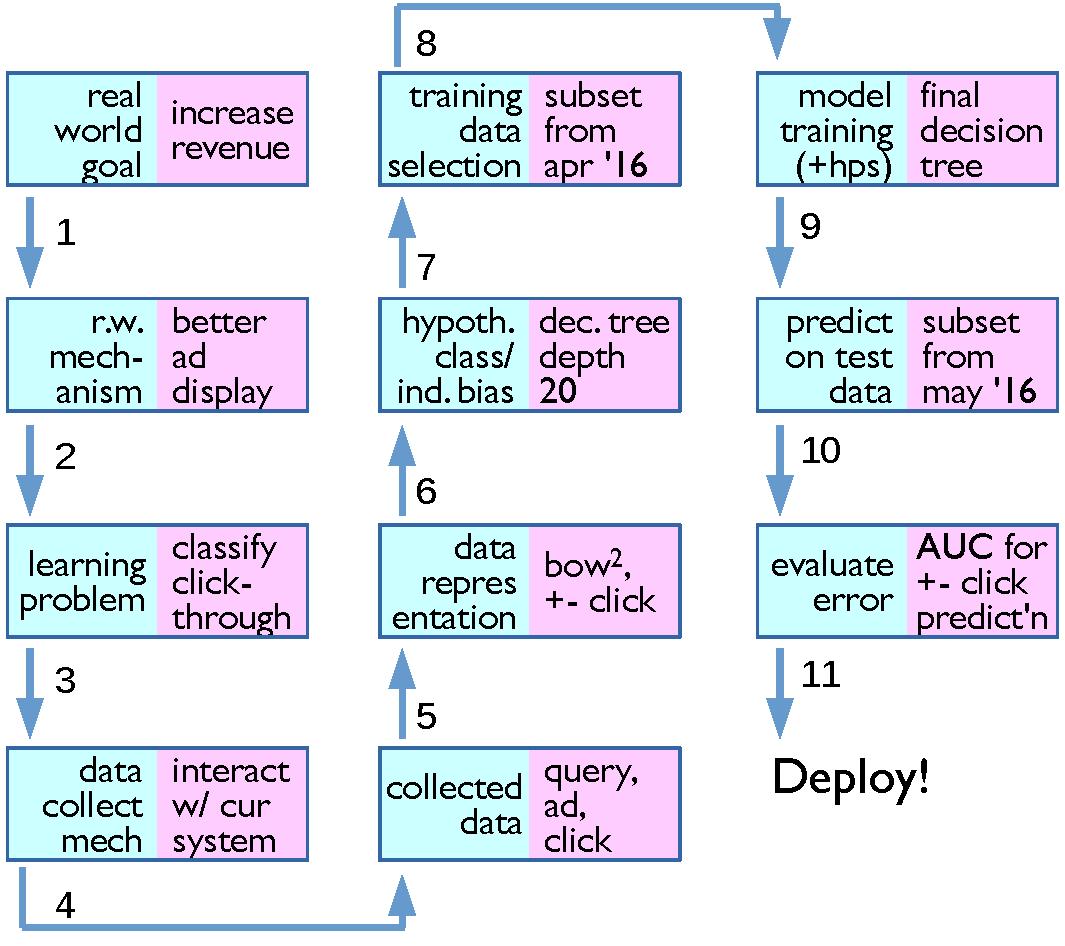
\includegraphics[width=1.5\textwidth]{figs/formal_deployml}
      \taburulecolor{darkblue}
      \tabulinestyle{1pt}
      \everyrow{\hline}
      \renewcommand{\arraystretch}{1.5}
      \hyphenpenalty=10000
      \exhyphenpenalty=10000
      \tabulinesep=2pt
      \begin{tabular}{|@{ }m{4mm}@{~~ }y@{~~~~}|@{}z|}
        1 & real world ~~~goal     & increase revenue        \\
        2 & real world mechanism& better ad display       \\
        3 & learning problem    & classify click-through  \\
        4 & data collection     & interaction w/ current system\\
        5 & collected data      & query, ad, click        \\
        6 & data representation & bow$^2$, $\pm$ click    \\
        7 & select model family   & decision trees, depth 20      \\
        8 & select training data   & subset from april'16    \\
        9 & train model \& hyperparams   & final decision tree     \\
       10 & predict on test data& subset from may'16      \\
       11 & evaluate error      & zero/one loss for $\pm$ click     \\
       12 & deploy! & (hope we achieve our goal)\\
      \end{tabular}
      \caption{A typical design process for a machine learning application.}
    \label{fig:formal_deployml}
    \end{centering}
  \end{marginfigure}
  \ResetNextFigure{}
}

In order to make these logs consumable by a machine learning algorithm, (6) we convert the data into input/output pairs: in this case, pairs of words from a bag-of-words representing the query and a bag-of-words representing the ad as input, and the click as a $\pm$ label. We then (7) select a model family (e.g., depth 20 decision trees), and thereby an inductive bias, for instance depth $\leq 20$ decision trees.

We're now ready to (8) select a specific subset of data to use as training data: in this case, data from April 2016. We split this into training and development and (9) learn a final decision tree, tuning the maximum depth on the development data. We can then use this decision tree to (10) make predictions on some held-out test data, in this case from the following month. We can (11) measure the overall quality of our predictor as zero/one loss (clasification error) on this test data and finally (12) deploy our system.

The important thing about this sequence of steps is that \emph{in any one, things can go wrong.} That is, between any two rows of this table, we are \emph{necessarily} accumulating some additional error against our original real world goal of increasing revenue. For example, in step 5, we decided on a representation that left out many possible variables we could have logged, like time of day or season of year. By leaving out those variables, we set an explicit upper bound on how well our learned system can do.

It is often an effective strategy to run an \concept{oracle experiment}. In an oracle experiment, we assume that everything below some line can be solved perfectly, and measure how much impact that will have on a higher line. As an extreme example, before embarking on a machine learning approach to the ad display problem, we should measure something like: if our classifier were \emph{perfect}, how much more money would we make? If the number is not very high, perhaps there is some better for our time.

Finally, although this sequence is denoted linearly, the entire process is highly interactive in practice. A large part of ``debugging'' machine learning (covered more extensively in Chapter~\ref{sec:prac} involves trying to figure out where in this sequence the biggest losses are and fixing that step. In general, it is often useful to \emph{build the stupidest thing that could possibly work}, then look at how well it's doing, and decide if and where to fix it.


\section{Further Reading}

TODO further reading


%%% Local Variables: 
%%% mode: latex
%%% TeX-master: "courseml"
%%% End: 

%\chapter{Geometry and Nearest Neighbors} \label{sec:knn}

\chapterquote{Our brains have evolved to get us out of the rain, find where the berries are, and keep us from getting killed. Our brains did not evolve to help us grasp really large numbers or to look at things in a hundred thousand dimensions.}{Ronald~Graham}


\begin{learningobjectives}
\item Describe a data set as points in a high dimensional space.
\item Explain the curse of dimensionality.
\item Compute distances between points in high dimensional space.
\item Implement a $K$-nearest neighbor model of learning.
\item Draw decision boundaries.
\item Implement the $K$-means algorithm for clustering.
\end{learningobjectives}

\dependencies{\chref{sec:dt}}

You can think of prediction tasks as mapping inputs
(course reviews) to outputs (course ratings).  As you learned in the
previous chapter, decomposing an input into a collection of features
(e.g., words that occur in the review) forms a useful abstraction for
learning.  Therefore, inputs are nothing more than lists of feature
values.  This suggests a \concept{geometric view} of data, where we
have one dimension for every feature.  In this view, examples are
points in a high-dimensional space.

Once we think of a data set as a collection of points in high
dimensional space, we can start performing geometric operations on
this data.  For instance, suppose you need to predict whether Alice
will like Algorithms.  Perhaps we can try to find another student who
is most ``similar'' to Alice, in terms of favorite courses.  Say this
student is Jeremy.  If Jeremy liked Algorithms, then we might guess
that Alice will as well.  This is an example of a \concept{nearest
  neighbor} model of learning.  By inspecting this model, we'll see a
completely different set of answers to the key learning questions we
discovered in \chref{sec:dt}.

\section{From Data to Feature Vectors}

An example is just a collection of feature values about that example,
for instance the data in Table~\ref{tab:data:course} from the Appendix.
To a person, these features have meaning.  One feature might count how
many times the reviewer wrote ``excellent'' in a course review.
Another might count the number of exclamation points.  A third might
tell us if any text is underlined in the review.

To a machine, the \concept{features} themselves have no meaning.  Only
the \concept{feature values}, and how they vary across examples, mean
something to the machine.  From this perspective, you can think about
an example as being represented by a \concept{feature vector}
consisting of one ``dimension'' for each feature, where each dimenion
is simply some real value.

Consider a review that said ``excellent'' three times, had one
exclamation point and no underlined text.  This could be represented
by the feature vector $\langle 3, 1, 0 \rangle$.  An almost identical
review that happened to have underlined text would have the feature
vector $\langle 3,1,1\rangle$.

Note, here, that we have imposed the convention that for
\concept{binary features} (yes/no features), the corresponding feature
values are $0$ and $1$, respectively.  This was an arbitrary choice.
We could have made them $0.92$ and $-16.1$ if we wanted.  But $0/1$ is
convenient and helps us interpret the feature values.  When we discuss
practical issues in Chapter~\ref{sec:prac}, you will see other reasons
why $0/1$ is a good choice.

\Figure{knn_projections}{A figure showing projections of data in two
  dimension in three ways -- see text.  Top: horizontal axis
  corresponds to the first feature (easy) and the vertical axis
  corresponds to the second feature (AI?); Middle: horizontal is
  second feature and vertical is third (systems?); Bottom: horizontal
  is first and vertical is third. Truly, the data points would like
  exactly on $(0,0)$ or $(1,0)$, etc., but they have been purturbed
  slightly to show duplicates.}

Figure~\ref{fig:knn_projections} shows the data from
Table~\ref{tab:data:course} in three views.  These three views are
constructed by considering two features at a time in different pairs.
In all cases, the plusses denote positive examples and the minuses
denote negative examples.  In some cases, the points fall on top of
each other, which is why you cannot see 20 unique points in all
figures.

\thinkaboutit{Match the example ids from Table~\ref{tab:data:course}
  with the points in Figure~\ref{fig:knn_projections}.}

The mapping from feature values to vectors is straighforward in the
case of real valued features (trivial) and binary features (mapped to
zero or one).  It is less clear what to do with \concept{categorical
  features}. For example, if our goal is to identify whether an object
in an image is a tomato, blueberry, cucumber or cockroach, we might
want to know its color: is it \categ{Red}, \categ{Blue}, \categ{Green}
or \categ{Black}?

One option would be to map \categ{Red} to a value of $0$, \categ{Blue}
to a value of $1$, \categ{Green} to a value of $2$ and \categ{Black}
to a value of $3$.  The problem with this mapping is that it turns an
unordered set (the set of colors) into an ordered set (the set
$\{0,1,2,3\}$).  In itself, this is not necessarily a bad thing.  But
when we go to \emph{use} these features, we will measure examples
based on their distances to each other.  By doing this mapping, we are
essentially saying that \categ{Red} and \categ{Blue} are more similar
(distance of $1$) than \categ{Red} and \categ{Black} (distance of
$3$).  This is probably not what we want to say!

A solution is to turn a categorical feature that can take four
different values (say: \categ{Red}, \categ{Blue}, \categ{Green} and
\categ{Black}) into four binary features (say: IsItRed?, IsItBlue?,
IsItGreen? and IsItBlack?).  In general, if we start from a
categorical feature that takes $V$ values, we can map it to $V$-many
binary indicator features.

\thinkaboutit{The computer scientist in you might be saying: actually
  we could map it to $\log_2 V$-many binary features!  Is this a good
  idea or not?}

With that, you should be able to take a data set and map each example
to a feature vector through the following mapping:

\begin{itemize}
\item Real-valued features get copied directly.
\item Binary features become $0$ (for false) or $1$ (for true).
\item Categorical features with $V$ possible values get mapped to
  $V$-many binary indicator features.
\end{itemize}

After this mapping, you can think of a single example as a
\concept{vector} in a high-dimensional \concept{feature space}.  If
you have $D$-many features (after expanding categorical features),
then this \concept{feature vector} will have $D$-many components.  We
will denote feature vectors as $\vec x = \langle x_1, x_2, \dots, x_D
\rangle$, so that $x_d$ denotes the value of the $d$th feature of
$\vec x$.  Since these are vectors with real-valued components in
$D$-dimensions, we say that they belong to the space $\R^D$.

For $D=2$, our feature vectors are just points in the plane, like in
Figure~\ref{fig:knn_projections}.  For $D=3$ this is three dimensional
space.  For $D>3$ it becomes quite hard to visualize.  (You should
resist the temptation to think of $D=4$ as ``time'' -- this will just
make things confusing.)  Unfortunately, for the sorts of problems you
will encounter in machine learning, $D \approx 20$ is considered ``low
dimensional,'' $D \approx 1000$ is ``medium dimensional'' and $D
\approx 100000$ is ``high dimensional.''

\thinkaboutit{Can you think of problems (perhaps ones already
  mentioned in this book!) that are low dimensional?  That are medium
  dimensional?  That are high dimensional?}

\section[K-Nearest Neighbors]{$K$-Nearest Neighbors}

The biggest advantage to thinking of examples as vectors in a high
dimensional space is that it allows us to apply geometric concepts to
machine learning.  For instance, one of the most basic things that one
can do in a vector space is compute \koncept{distances}{distance}.  In
two-dimensional space, the distance between $\langle 2,3\rangle$ and
$\langle 6,1\rangle$ is given by $\sqrt{(2-6)^2 + (3-1)^2} = \sqrt{18}
\approx 4.24$.  In general, in $D$-dimensional space, the
\concept{Euclidean distance} between vectors $\vec a$ and $\vec b$ is
given by Eq~\eqref{eq:euclidean} (see Figure~\ref{fig:knn_euclidean}
for geometric intuition in three dimensions):


\begin{equation} \label{eq:euclidean}
d(\vec a, \vec b) = \left[ \sum_{d=1}^D (a_d - b_d)^2 \right]^{\frac 1 2}
\end{equation}

\Figure{knn_euclidean}{A figure showing Euclidean distance in
  three dimensions. The length of the green segments are $0.6$, $0.6$ and $0.3$ respectively, in the x-, y-, and z-axes. The total distance between the red dot and the orange dot is therefore $\sqrt{0.6^2 + 0.6^2 + 0.3^2} = 0.9$.}

\thinkaboutit{Verify that $d$ from Eq~\eqref{eq:euclidean} gives the
  same result ($4.24$) for the previous computation.}

\Figure{knn_classifyit}{A figure showing an easy NN classification
  problem where the test point is a ? and should be negative.}

Now that you have access to distances between examples, you can start
thinking about what it means to learn again.  Consider
Figure~\ref{fig:knn_classifyit}.  We have a collection of training
data consisting of positive examples and negative examples.  There is
a test point marked by a question mark.  Your job is to guess the
correct label for that point.

Most likely, you decided that the label of this test point is
positive.  One reason why you might have thought that is that you
believe that the label for an example should be similar to the label
of nearby points.  This is an example of a new form of
\concept{inductive bias}.

The \concept{nearest neighbor} classifier is build upon this insight.
In comparison to decision trees, the algorithm is ridiculously
simple.  At training time, we simply store the entire training set.
At test time, we get a test example $\hat\vx$.  To predict its label,
we find the training example $\vx$ that is most similar to $\hat\vx$.
In particular, we find the training example $\vx$ that
\emph{minimizes} $d(\vx,\hat\vx)$.  Since $\vx$ is a training example,
it has a corresponding label, $y$.  We predict that the label of
$\hat\vx$ is also $y$.

Despite its simplicity, this nearest neighbor classifier is incredibly
effective.  (Some might say \emph{frustratingly} effective.)  However,
it is particularly prone to overfitting label noise.  Consider the
data in Figure~\ref{fig:knn_classifyitbad}.  You would probably want
to label the test point positive.  Unfortunately, it's nearest
neighbor happens to be negative.  Since the nearest neighbor algorithm
only looks at the \emph{single} nearest neighbor, it cannot consider
the ``preponderance of evidence'' that this point should probably
actually be a positive example.  It will make an unnecessary error.

\Figure{knn_classifyitbad}{A figure showing an easy NN
  classification problem where the test point is a ? and should be
  positive, but its NN is actually a negative point that's noisy.}


A solution to this problem is to consider more than just the single
nearest neighbor when making a classification decision.  We can
consider the \koncept{$K$-nearest neighbors}{K-nearest neighbors} and
let them \concept{vote} on the correct class for this test point.  If
you consider the $3$-nearest neighbors of the test point in
Figure~\ref{fig:knn_classifyitbad}, you will see that two of them are
positive and one is negative.  Through voting, positive would win.

\thinkaboutit{Why is it a good idea to use an odd number for $K$?}

\newalgorithm%
  {knn:knn}%
  {\FUN{KNN-Predict}(\VAR{$\mat D$}, \VAR{K}, \VAR{$\hat\vx$})}
  {
\SETST{S}{\emptylist}
\FOR{\VAR{$n$} $=\CON{1}$ \TO \VAR{$N$}}
\SETST{S}{\VAR{S} \pushlist{$\langle$d(\VAR{$\vx_n$}, \VAR{$\hat\vx$}), \VAR{n}$\rangle$}} \COMMENT{store distance to training example $n$}
\ENDFOR
\SETST{S}{\FUN{sort}(\VAR{S})} \COMMENT{put lowest-distance objects first}
\SETST{$\hat y$}{\CON{0}}
\FOR{\VAR{k} $=\CON{1}$ \TO \VAR{K}}
\SETST{$\langle$dist,n$\rangle$}{\VAR{S$_k$}} \COMMENT{$n$ this is the $k$th closest data point}
\SETST{$\hat y$}{\VAR{$\hat y$} $+$ \VAR{$y_n$}} \COMMENT{vote
  according to the label for the $n$th training point}
\ENDFOR
\RETURN \FUN{sign}(\VAR{$\hat y$}) \COMMENT{return $+1$ if $\hat y>0$
  and $-1$ if $\hat y<0$}
}

The full algorithm for $K$-nearest neighbor classification is given in
Algorithm~\ref{alg:knn:knn}.  Note that there actually is no
``training'' phase for $K$-nearest neighbors.  In this algorithm we
have introduced five new conventions:

\begin{enumerate}
\item The training data is denoted by \VAR{$\mat D$}.
\item We assume that there are $N$-many training examples.
\item These examples are pairs $(\vx_1,y_1), (\vx_2,y_2), \dots,
  (\vx_N,y_N)$.\\(Warning: do not confuse $\vx_n$, the $n$th training
  example, with $x_d$, the $d$th feature for example $\vx$.)
\item We use \emptylist to denote an empty list and \pushlist{$\cdot$}
  to append $\cdot$ to that list.
\item Our prediction on $\hat\vx$ is called $\hat y$.
\end{enumerate}

The first step in this algorithm is to compute distances from the test
point to all training points (lines 2-4).  The data points are then
sorted according to distance.  We then apply a clever trick of
\emph{summing} the class labels for each of the $K$ nearest neighbors
(lines 6-10) and using the \FUN{sign} of this sum as our prediction.

\thinkaboutit{Why is the sign of the sum computed in lines 2-4 the
  same as the majority vote of the associated training examples?}

The big question, of course, is how to choose $K$.  As we've seen,
with $K=1$, we run the risk of overfitting.  On the other hand, if $K$
is large (for instance, $K=N$), then \FUN{KNN-Predict} will always
predict the majority class.  Clearly that is underfitting.  So, $K$ is
a hyperparameter of the KNN algorithm that allows us to trade-off
between overfitting (small value of $K$) and underfitting (large value
of $K$).

\thinkaboutit{Why can't you simply pick the value of $K$ that does
  best on the training data?  In other words, why do we have to treat
  it like a hyperparameter rather than just a parameter.}

One aspect of \concept{inductive bias} that we've seen for KNN is that
it assumes that nearby points should have the same label.  Another
aspect, which is quite different from decision trees, is that all
features are equally important!  Recall that for decision trees, the
key question was \emph{which features are most useful for
  classification?}  The whole learning algorithm for a decision tree
hinged on finding a small set of good features.  This is all thrown
away in KNN classifiers: every feature is used, and they are all used
the same amount.  This means that if you have data with only a few
relevant features and lots of irrelevant features, KNN is likely to do
poorly.

\MoveNextFigure{-18cm}
\Figure{knn:ski}{A figure of a ski and a snowboard.}

\MoveNextFigure{-10cm}
\Figure{knn:skidata}{Classification data for ski vs snowboard in
  2d}

A related issue with KNN is \concept{feature scale}.  Suppose that we
are trying to classify whether some object is a ski or a snowboard
(see Figure~\ref{fig:knn:ski}).  We are given two features about this
data: the width and height.  As is standard in skiing, width is
measured in millimeters and height is measured in centimeters.  Since
there are only two features, we can actually plot the entire training
set; see Figure~\ref{fig:knn:skidata} where ski is the positive class.
Based on this data, you might guess that a KNN classifier would do
well.

Suppose, however, that our measurement of the width was computed in
millimeters (instead of centimeters).  This yields the data shown in
Figure~\ref{fig:knn:skidatabad}.  Since the width values are now tiny,
in comparison to the height values, a KNN classifier will effectively
\emph{ignore} the width values and classify almost purely based on
height.  The predicted class for the displayed test point had changed
because of this feature scaling.

\MoveNextFigure{-5cm}
\Figure{knn:skidatabad}{Classification data for ski vs snowboard in
  2d, with width rescaled to mm.}


We will discuss feature scaling more in Chapter~\ref{sec:prac}.  For
now, it is just important to keep in mind that KNN does not have the
power to decide which features are important.

\begin{mathreview}{Vector Arithmetic and Vector Norms}
  A (real-valued) \textbf{vector} is just an array of real values, for
  instance $\vx = \langle 1, 2.5, -6 \rangle$ is a three-dimensional
  vector. In general, if $\vx = \langle x_1, x_2, \dots, x_D \rangle$,
  then $x_d$ is it's $d$th component. So $x_3 = -6$ in the previous
  example.
  
~

  \textbf{Vector sums} are computed pointwise, and are only defined when
  dimensions match, so $\langle 1, 2.5, -6 \rangle + \langle 2, -2.5,
  3 \rangle = \langle 3, 0, -3 \rangle$. In general, if $\vec c = \vec
  a + \vec b$ then $c_d = a_d + b_d$ for all $d$. Vector addition can
  be viewed geometrically as taking a vector $\vec a$, then tacking on
  $\vec b$ to the end of it; the new end point is exactly $\vec c$.

~

  Vectors can be \textbf{scaled} by real values; for instance $2
  \langle 1, 2.5, -6 \rangle = \langle 2, 5, -12 \rangle$; this is
  called scalar multiplication. In general, $a \vx = \langle a x_1, a
  x_2, \dots, a x_D \rangle$.

~

  The \textbf{norm} of a vector $\vx$, written $\norm{\vx}$ is its
  length. Unless otherwise specified, this is its \emph{Euclidean}
  length, namely: $\norm{\vx} = \sqrt{\sum_d x_d^2}$.
\end{mathreview}

\section{Decision Boundaries}

The standard way that we've been thinking about learning algorithms up
to now is in the \emph{query model}.  Based on training data, you
learn something.  I then give you a query example and you have to
guess it's label.

\Figure{knn:db}{decision boundary for 1nn.}

An alternative, less passive, way to think about a learned model is to
ask: what sort of test examples will it classify as positive, and what
sort will it classify as negative.  In Figure~\ref{fig:knn:db}, we have a
set of training data.  The background of the image is colored blue in
regions that \emph{would} be classified as positive (if a query were
issued there) and colored red in regions that \emph{would} be
classified as negative.  This coloring is based on a $1$-nearest
neighbor classifier.

In Figure~\ref{fig:knn:db}, there is a solid line separating the positive
regions from the negative regions.  This line is called the
\concept{decision boundary} for this classifier.  It is the line with
positive land on one side and negative land on the other side.

\Figure{knn:db3}{decision boundary for knn with k=3.}

Decision boundaries are useful ways to visualize the
\concept{complexity} of a learned model.  Intuitively, a learned model
with a decision boundary that is really jagged (like the coastline of
Norway) is really complex and prone to overfitting.  A learned model
with a decision boundary that is really simple (like the bounary
between Arizona and Utah) is potentially underfit. 
%In
%Figure~\ref{fig:knn:dbmany}, you can see the decision boundaries for KNN
%models with $K \in \{1, 3, 5, 7\}$.  As you can see, the boundaries
%become simpler and simpler as $K$ gets bigger.

Now that you know about decision boundaries, it is natural to ask:
what do decision boundaries for decision trees look like?  In order to
answer this question, we have to be a bit more formal about how to
build a decision tree on real-valued features.  (Remember that the
algorithm you learned in the previous chapter implicitly assumed
\emph{binary} feature values.)  The idea is to allow the decision tree
to ask questions of the form: ``is the value of feature $5$ greater
than $0.2$?''  That is, for real-valued features, the decision tree
nodes are parameterized by a feature and a threshold for that
feature.  An example decision tree for classifying skis versus
snowboards is shown in Figure~\ref{fig:knn:dtski}.

\Figure{knn:dtski}{decision tree for ski vs. snowboard}

\Figure{knn:dtdb}{decision boundary for dt in previous figure}

Now that a decision tree can handle feature vectors, we can talk about
decision boundaries.  By example, the decision boundary for the
decision tree in Figure~\ref{fig:knn:dtski} is shown in
Figure~\ref{fig:knn:dtdb}.  In the figure, space is first split in half
according to the first query along one axis.  Then, depending on which
half of the space you look at, it is either split again along the
other axis, or simply classified.

%\TODOFigure{knn:dtdeepdb}{decision boundary for deep dt on ski data}

Figure~\ref{fig:knn:dtdb} is a good visualization of decision boundaries
for decision trees in general.  Their decision boundaries are
axis-aligned cuts.  The cuts must be axis-aligned because nodes can
only query on a single feature at a time.  In this case, since the
decision tree was so shallow, the decision boundary was relatively
simple.  

\thinkaboutit{What sort of data might yield a very simple decision
  boundary with a decision tree and very complex decision boundary
  with 1-nearest neighbor?  What about the other way around?}

\section[K-Means Clustering]{$K$-Means Clustering}
\label{sec:knn:kmeans}

Up through this point, you have learned all about supervised learning
(in particular, binary classification).  As another example of the use
of geometric intuitions and data, we are going to temporarily consider
an \concept{unsupervised learning} problem.  In unsupervised learning,
our data consists \emph{only} of examples $\vx_n$ and does \emph{not}
contain corresponding labels.  Your job is to make sense of this data,
even though no one has provided you with correct labels.  The
particular notion of ``making sense of'' that we will talk about now
is the \concept{clustering} task.

\Figure{knn:clustering}{simple clustering data... clusters in UL,
  UR and BC.}

Consider the data shown in Figure~\ref{fig:knn:clustering}.  Since
this is unsupervised learning and we do not have access to labels, the
data points are simply drawn as black dots.  Your job is to split this
data set into three clusters.  That is, you should label each data
point as \categ{A}, \categ{B} or \categ{C} in whatever way you want.

For this data set, it's pretty clear what you should do.  You probably
labeled the upper-left set of points \categ{A}, the upper-right set of
points \categ{B} and the bottom set of points \categ{C}.  Or perhaps
you permuted these labels.  But chances are your clusters were the
same as mine.

The $K$-means clustering algorithm is a particularly simple and
effective approach to producing clusters on data like you see in
Figure~\ref{fig:knn:clustering}.  The idea is to represent each
cluster by it's cluster center.  Given cluster centers, we can simply
assign each point to its nearest center.  Similarly, if we know the
assignment of points to clusters, we can compute the centers.  This
introduces a chicken-and-egg problem.  If we knew the clusters, we
could compute the centers.  If we knew the centers, we could compute
the clusters.  But we don't know either.

\Figure{knn:kmeans}{first few iterations of k-means running on
  previous data set}

The general computer science answer to chicken-and-egg problems is
\concept{iteration}.  We will start with a guess of the cluster
centers.  Based on that guess, we will assign each data point to its
closest center.  Given these new assignments, we can recompute the
cluster centers.  We repeat this process until clusters stop moving.
The first few iterations of the $K$-means algorithm are shown in
Figure~\ref{fig:knn:kmeans}.  In this example, the clusters converge
very quickly.

\newalgorithm%
  {knn:kmeans}%
  {\FUN{K-Means}(\VAR{$\mat D$}, \VAR{K})}
  {
\FOR{$\VAR{k} = \CON{1}$ \TO $\VAR{K}$}
\SETST{$\vec\mu_k$}{some random location} \COMMENT{randomly initialize
  center for $k$th cluster}
\ENDFOR
\REPEAT
\FOR{$\VAR{n} = \CON{1}$ \TO $\VAR{N}$}
\SETST{$z_n$}{$\argmin_k \norm{\vec\mu_k - \vx_n}$}
  \COMMENT{assign example $n$ to closest center}
\ENDFOR
\FOR{$\VAR{k} = \CON{1}$ \TO $\VAR{K}$}
\SETST{$\mat X_k$}{$\{$ \VAR{$\vx_n$} : \VAR{$z_n$} = \VAR{$k$} $\}$}
  \COMMENT{points assigned to cluster $k$}
\SETST{$\vec\mu_k$}{\FUN{mean}(\VAR{$\mat X_k$})}
  \COMMENT{re-estimate center of cluster $k$}
\ENDFOR
\UNTIL{\VAR{$\vec\mu$}s stop changing}
\RETURN \VAR{$\vec z$} \COMMENT{return cluster assignments}
}

Algorithm~\ref{alg:knn:kmeans} spells out the $K$-means clustering
algorithm in detail.  The cluster centers are initialized randomly.
In line 6, data point $\vx_n$ is compared against each cluster center
$\vec\mu_k$.  It is assigned to cluster $k$ if $k$ is the center with
the smallest distance.  (That is the ``$\argmin$'' step.)  The
variable \VAR{$z_n$} stores the assignment (a value from $1$ to $K$)
of example $n$.  In lines 8-12, the cluster centers are re-computed.
First, $\mat X_k$ stores all examples that have been assigned to
cluster $k$.  The center of cluster $k$, \VAR{$\vec\mu_k$} is then
computed as the mean of the points assigned to it.  This process
repeats until the centers converge.

An obvious question about this algorithm is: does it converge?  A
second question is: how long does it take to converge.  The first
question is actually easy to answer.  Yes, it does.  And in practice,
it usually converges quite quickly (usually fewer than $20$
iterations).  In Chapter~\ref{sec:unsup}, we will actually
\emph{prove} that it converges.  The question of how long it takes to
converge is actually a really interesting question.  Even though the
$K$-means algorithm dates back to the mid 1950s, the best known
convergence rates were \emph{terrible} for a long time.  Here,
terrible means exponential in the number of data points.  This was a
sad situation because empirically we knew that it converged very
quickly.  New algorithm analysis techniques called ``smoothed
analysis'' were invented in 2001 and have been used to show very fast
convergence for $K$-means (among other algorithms).  These techniques
are well beyond the scope of this book (and this author!) but suffice
it to say that $K$-means is fast in practice and is provably fast in
theory.

%\TODOFigure{knn:kmeansbad}{first few iterations of k-means running on
%  previous data set with BAD initialization}

It is important to note that although $K$-means is guaranteed to
converge and guaranteed to converge quickly, it is \emph{not}
guaranteed to converge to the ``right answer.''  The key problem with
unsupervised learning is that we have no way of knowing what the
``right answer'' is.  Convergence to a bad solution is usually due to
poor initialization. 
%For example, poor initialization in the data set
%from before yields convergence like that seen in
%Figure~\ref{fig:knn:kmeansbad}.  As you can see, the algorithm
%\emph{has} converged.  It has just converged to something less than
%satisfactory.

\thinkaboutit{What is the difference between unsupervised and
  supervised learning that means that we know what the ``right
  answer'' is for supervised learning but not for unsupervised
  learning?}

\section{Warning: High Dimensions are Scary}

Visualizing one hundred dimensional space is incredibly difficult for
humans.  After huge amounts of training, some people have reported
that they can visualize four dimensional space in their heads.  But
beyond that seems impossible.\sidenote{If you want to try to get an
  intuitive sense of what four dimensions looks like, I highly
  recommend the short 1884 book \emph{Flatland: A Romance of Many
    Dimensions} by Edwin Abbott Abbott.  You can even read it online
  at \url{gutenberg.org/ebooks/201}.}

In addition to being hard to visualize, there are at least two
additional problems in high dimensions, both refered to as
\concept{the curse of dimensionality}.  One is computational, the
other is mathematical.

\Figure{knn:grid:2d}{2d knn with an overlaid grid, cell with test
  point highlighted}

From a computational perspective, consider the following problem.
For $K$-nearest neighbors, the speed of prediction is slow for a very
large data set.  At the very least you have to look at every training
example every time you want to make a prediction.  To speed things up
you might want to create an \emph{indexing} data structure.  You can
break the plane up into a grid like that shown in
Figure~\ref{fig:knn:grid:2d}.  Now, when the test point comes in, you can
quickly identify the grid cell in which it lies.  Now, instead of
considering \emph{all} training points, you can limit yourself to
training points \emph{in that grid cell} (and perhaps the neighboring
cells).  This can potentially lead to huge computational savings.

In two dimensions, this procedure is effective.  If we want to break
space up into a grid whose cells are $0.2 \times 0.2$, we can clearly
do this with $25$ grid cells in two dimensions (assuming the range of
the features is $0$ to $1$ for simplicity).  In three dimensions,
we'll need $125 = 5 \times 5 \times 5$ grid cells.  In four
dimensions, we'll need $625$.  By the time we get to ``low
dimensional'' data in $20$ dimensions, we'll need $95,367,431,640,625$
grid cells (that's $95$ trillion, which is about $6$ to $7$ times the
US national debt as of January 2011).  So if you're in $20$
dimensions, this gridding technique will only be useful if you have at
least $95$ trillion training examples.

For ``medium dimensional'' data (approximately $1000$) dimesions, the
number of grid cells is a $9$ followed by $698$ numbers before the
decimal point.  For comparison, the number of atoms in the universe is
approximately $1$ followed by $80$ zeros.  So even if each atom
yielded a googul training examples, we'd still have far fewer
examples than grid cells.  For ``high dimensional'' data
(approximately $100000$) dimensions, we have a $1$ followed by just
under $70,000$ zeros.  Far too big a number to even really comprehend.

Suffice it to say that for even moderately high dimensions, the amount
of computation involved in these problems is enormous.

\thinkaboutit{How does the above analysis relate to the number of data
  points you would need to fill out a full decision tree with $D$-many
  features?  What does this say about the importance of shallow
  trees?}

In addition to the computational difficulties of working in high
dimensions, there are a large number of strange mathematical
occurances there.  In particular, many of your intuitions that you've
built up from working in two and three dimensions just do not carry
over to high dimensions.  We will consider two effects, but there are
countless others.  The first is that high dimensional spheres look
more like porcupines than like balls.\sidenote{This result was
  related to me by Mark Reid, who heard about it from Marcus Hutter.}
The second is that distances between points in high dimensions are all
approximately the same.

\Figure{knn:cursetwo}{2d spheres in spheres}

Let's start in two dimensions as in Figure~\ref{fig:knn:cursetwo}.
We'll start with four green spheres, each of radius one and each
touching exactly two other green spheres.  (Remember that in two
dimensions a ``sphere'' is just a ``circle.'')  We'll place a red
sphere in the middle so that it touches all four green spheres.  We
can easily compute the radius of this small sphere.  The pythagorean
theorem says that $1^2 + 1^2 = (1+r)^2$, so solving for $r$ we get $r
= \sqrt 2 - 1 \approx 0.41$.  Thus, by calculation, the blue sphere
lies entirely within the cube (cube = square) that contains the grey
spheres.  (Yes, this is also obvious from the picture, but perhaps you
can see where this is going.)

\Figure{knn:cursethree}{3d spheres in spheres}

Now we can do the same experiment in three dimensions, as shown in
Figure~\ref{fig:knn:cursethree}.  Again, we can use the pythagorean
theorem to compute the radius of the blue sphere.  Now, we get $1^2 +
1^2 + 1^2 = (1+r)^2$, so $r = \sqrt3 - 1 \approx 0.73$.  This is still
entirely enclosed in the cube of width four that holds all eight grey
spheres.

At this point it becomes difficult to produce figures, so you'll have
to apply your imagination.  In four dimensions, we would have $16$
green spheres (called \concept{hyperspheres}), each of radius one.
They would still be inside a cube (called a \concept{hypercube}) of
width four.  The blue hypersphere would have radius $r = \sqrt4 - 1 =
1$.  Continuing to five dimensions, the blue hypersphere embedded in
$256$ green hyperspheres would have radius $r = \sqrt5-1 \approx 1.23$
and so on.

In general, in $D$-dimensional space, there will be $2^D$ green
hyperspheres of radius one.  Each green hypersphere will touch exactly
$n$-many other hyperspheres.  The blue hyperspheres in the middle will
touch them all and will have radius $r = \sqrt D - 1$.

Think about this for a moment.  As the number of dimensions grows, the
radius of the blue hypersphere \emph{grows without bound!}.  For
example, in $9$-dimensions the radius of the blue hypersphere is now
$\sqrt9-1 = 2$.  But with a radius of two, the blue hypersphere is now
``squeezing'' between the green hypersphere and \emph{touching} the
edges of the hypercube.  In $10$ dimensional space, the radius is
approximately $2.16$ and it pokes outside the cube.

%\Figure{knn:porcupine}{porcupine versus ball}

%This is why we say that high dimensional spheres look like porcupines
%and not balls (see Figure~\ref{fig:knn:porcupine}).  The moral of this
%story from a \emph{machine learning} perspective is that intuitions
%you have about space might not carry over to high dimensions.  For
%example, what you think looks like a ``round'' cluster in two or three
%dimensions, might not look so ``round'' in high dimensions.

%\Figure{knn:uniform}{100 uniform random points in 1, 2 and 3
%  dimensions}

The second strange fact we will consider has to do with the distances
between points in high dimensions.  We start by considering random
points in one dimension.  That is, we generate a fake data set
consisting of $100$ random points between zero and one.  We can do the
same in two dimensions and in three dimensions.  See
Figure~\ref{fig:knn:uniform} for data distributed uniformly on the
\concept{unit hypercube} in different dimensions.

Now, pick two of these points at random and compute the distance
between them.  Repeat this process for all pairs of points and average
the results.  For the data shown in Figure~\ref{fig:knn:uniform}, the
average distance between points in one dimension is about $0.346$; in two
dimensions is about $0.518$; and in three dimensions is $0.615$. The fact that these \emph{increase} as the dimension increases is not surprising. The furthest two points can be in a 1-dimensional hypercube (line) is $1$; the furthest in a 2-dimensional hypercube (square) is $\sqrt 2$ (opposite corners); the furthest in a 3-d hypercube is $\sqrt 3$ and so on. In general, the furthest two points in a $D$-dimensional hypercube will be $\sqrt D$.

You can actually compute these values analytically.  Write $\Uni_D$ for
the uniform distribution in $D$ dimensions.  The quantity we are
interested in computing is:
\begin{equation} \label{eq:knn:dist}
  \textit{avgDist}(D)
  = \Ep_{\vec a \sim \Uni_D} \Big[
    \Ep_{\vec b \sim \Uni_D} \Big[
      \norm{\vec a - \vec b}
      \Big] \Big]
\end{equation}
We can actually compute this in closed form and arrive
at $\textit{avgDist}(D) = \sqrt D / 3$. Because we know that the maximum distance between two points grows like $\sqrt D$, this says that the ratio between average distance and maximum distance converges to $1/3$. 

What is more interesting, however, is the \emph{variance} of the distribution of distances. You can show that in $D$ dimensions, the variance is \emph{constant} $1/\sqrt{18}$, \emph{independent of $D$}. This means that when you look at (variance) divided-by (max distance), the variance behaves like $1/\sqrt{18 D}$, which means that the effective variance continues to shrink as $D$ grows\mycite{brin95nn}.

\Figure{knn:uniformhist}{histogram of distances in D=2,8,32,128,512}

When I first saw and re-proved this result, I was skeptical, as I
imagine you are.  So I implemented it.  In
Figure~\ref{fig:knn:uniformhist} you can see the results.  This
presents a \emph{histogram} of distances between random points in $D$
dimensions for $D \in \{1,2,3,10,20,100\}$.  As you can see, all of
these distances begin to concentrate around $0.4\sqrt{D}$, even for ``medium
dimension'' problems.

You should now be terrified: the only bit of information that KNN gets
is distances.  And you've just seen that in moderately high dimensions,
all distances becomes equal.  So then isn't it the case that KNN
simply cannot work?

\TODOFigure{knn:mnist}{histogram of distances in multiple D for mnist}

The answer has to be no.  The reason is that the data that we get is
\emph{not} uniformly distributed over the unit hypercube.  We can see
this by looking at two real-world data sets.  The first is an image
data set of hand-written digits (zero through nine); see
Section~\ref{sec:data:mnist}.  Although this data is originally in
$256$ dimensions ($16$ pixels by $16$ pixels), we can artifically
reduce the dimensionality of this data.  In Figure~\ref{fig:knn:mnist}
you can see the histogram of average distances between points in this
data at a number of dimensions.

As you can see from these histograms, distances have \emph{not}
concentrated around a single value.  This is very good news: it means
that there is hope for learning algorithms to work!  Nevertheless, the
moral is that high dimensions are weird.


% \section{Extensions to KNN}

% There are several fundamental problems with KNN classifiers.  First,
% some neighbors might be ``better'' than others.  Second, test-time
% performance scales badly as your number of training examples
% increases.  Third, it treats each dimension independently.  We will
% not address the third issue, as it has not really been solved (though
% it makes a great thought question!).

% \Figure{knn:badneighbors}{data set with 5nn, test point closest to
%   two negatives, then to three far positives}

% Regarding neighborliness, consider Figure~\ref{fig:knn:badneighbors}.
% Using $K=5$ nearest neighbors, the test point would be classified as
% positive.  However, we might actually believe that it should be
% classified negative because the two negative neighbors are \emph{much}
% closer than the three positive neighbors.

% \Figure{knn:badneighbors2}{same as previous with $\ep$ ball}

% There are at least two ways of addressing this issue.  The first is
% the \concept{$\ep$-ball} solution.  Instead of connecting each data
% point to some fixed number ($K$) of nearest neighbors, we simply
% connect it to \emph{all} neighbors that fall within some ball of
% radius $\ep$.  Then, the majority class of all the points in the $\ep$
% ball wins.  In the case of a tie, you would have to either guess, or
% report the majority class.  Figure~\ref{fig:knn:badneighbors2} shows an
% $\ep$ ball around the test point that happens to yield the proper
% classification.

% When using $\ep$-ball nearest neighbors rather than KNN, the
% hyperparameter changes from $K$ to $\ep$.  You would need to set it in
% the same way as you would for KNN.

% \thinkaboutit{One issue with $\ep$-balls is that the $\ep$-ball for
%   some test point might be empty.  How would you handle this?}

% An alternative to the $\ep$-ball solution is to do \concept{weighted
%   nearest neighbors}.  The idea here is to still consider the
% $K$-nearest neighbors of a test point, but give them uneven votes.
% Closer points get more vote than further points.  When classifying a
% point $\hat\vx$, the usual strategy is to give a training point
% $\vx_n$ a vote that decays exponentially in the distance between
% $\hat\vx$ and $\vx_n$.  Mathematically, the vote that neighbor $n$
% gets is:
% \begin{equation} \label{eq:expdecay}
% \exp\left[ - \frac 1 2 \norm{\hat\vx - \vx_n}^2 \right]
% \end{equation}
% Thus, nearby points get a vote very close to $1$ and far away points
% get a vote very close to $0$.  The overall prediction is positive if
% the sum of votes from positive neighbors outweighs the sum of votes
% from negative neighbors.

% \thinkaboutit{Could you combine the $\ep$-ball idea with the weighted
%   voting idea?  Does it make sense, or does one idea seem to trump the
%   other?}

% The second issue with KNN is scaling.  To predict the label of a
% single test point, we need to find the $K$ nearest neighbors of that
% test point in the training data.  With a standard implementation, this
% will take $\cO(N D + K \log K)$ time\sidenote{The $ND$ term comes from
%   computing distances between the test point and all training points.
%   The $K\log K$ term comes from finding the $K$ smallest values in the
%   list of distances, using a median-finding algorithm.  Of course,
%   $ND$ almost always dominates $K\log K$ in practice.}.  For very
% large data sets, this is impractical.

% \TODOFigure{knn:collapse}{two figures of points collapsed to mean, one
%   with good results and one with dire results}

% A first attempt to speed up the computation is to represent each class
% by a \emph{representative.}  A natural choice for a representative
% would be the mean.  We would collapse all positive examples down to
% their mean, and all negative examples down to their mean.  We could
% then just run $1$-nearest neighbor and check whether a test point is
% closer to the mean of the positive points or the mean of the negative
% points.  Figure~\ref{fig:knn:collapse} shows an example in which this
% would probably work well, and an example in which this would probably
% work poorly.  The problem is that collapsing each class to its mean is
% too aggressive.

% \TODOFigure{knn:collapse2}{data from previous bad case collapsed into
%   L=2 cluster and test point classified based on means and $1$-nn}

% A less aggressive approach is to make use of the $K$-means algorithm
% for clustering.  You can cluster the positive examples into $L$
% clusters (we are using $L$ to avoid variable overloading!) and then
% cluster the negative examples into $L$ separate clusters.  This is
% shown in Figure~\ref{fig:knn:collapse2} with $L=2$.  Instead of storing the
% entire data set, you would only store the \emph{means} of the $L$
% positive clusters and the means of the $L$ negative clusters.  At test
% time, you would run the $K$-nearest neighbors algorithm against these
% \emph{means} rather than against the full training set.  This leads to
% a much faster runtime of just $\cO(L D + K \log K)$, which is probably
% dominated by $LD$.

% \thinkaboutit{Clustering of classes was introduced as a way of making
%   things faster.  Will it make things worse, or could it help?}

\section{Further Reading}

TODO further reading



\begin{comment}
Similarities versus distances
Relationship to databases
Underfitting/overfitting by k
Weighted voting
From two classes to M classes
Decision boundaries for knn versus dts
Computational complexity
Reducing each class to one point: means
K-means clustering
\end{comment}

%%% Local Variables: 
%%% mode: latex
%%% TeX-master: "courseml"
%%% End: 

%\chapter{The Perceptron} \label{sec:perc}

\chapterquote{Algebra is nothing more than geometry, in words; geometry is nothing more than algebra, in pictures.}{Sophie~Germain}


\begin{learningobjectives}
\item Describe the biological motivation behind the perceptron.
\item Classify learning algorithms based on whether they are
  error-driven or not.
\item Implement the perceptron algorithm for binary classification.
\item Draw perceptron weight vectors and the corresponding decision
  boundaries in two dimensions.
%\item Define linear separability, and be able to turn any arbitrary
%  data set into a linearly separable data set.
\item Contrast the decision boundaries of decision trees, nearest
  neighbor algorithms and perceptrons.
\item Compute the margin of a given weight vector on a given data set.
\end{learningobjectives}

\dependencies{\chref{sec:dt}, \chref{sec:knn}}

\newthought{So far, you've seen two types} of learning models: in
decision trees, only a small number of features are used to make
decisions; in nearest neighbor algorithms, all features are used
equally.  Neither of these extremes is always desirable.  In some
problems, we might want to use most of the features, but use some more
than others.

In this chapter, we'll discuss the \concept{perceptron} algorithm for
learning \concept{weights} for features.  As we'll see, learning
weights for features amounts to learning a \concept{hyperplane}
classifier: that is, basically a division of space into two halves by
a straight line, where one half is ``positive'' and one half is
``negative.''  In this sense, the perceptron can be seen as explicitly
finding a good \concept{linear decision boundary}.

\section{Bio-inspired Learning}

\Figure{perc:neuron}{a picture of a neuron}

Folk biology tells us that our brains are made up of a bunch of little
units, called \concept{neurons}, that send electrical signals to one
another.  The \emph{rate} of firing tells us how ``activated'' a
neuron is.  A single neuron, like that shown in
Figure~\ref{fig:perc:neuron} might have three incoming neurons.  These
incoming neurons are firing at different rates (i.e., have different
\concept{activations}).  Based on how much these incoming neurons are
firing, and how ``strong'' the neural connections are, our main neuron
will ``decide'' how strongly it wants to fire.  And so on through the
whole brain.  Learning in the brain happens by neurons becomming
connected to other neurons, and the strengths of connections adapting
over time.

\Figure{perc:example}{figure showing feature vector and weight
  vector and products and sum}

The real biological world is much more complicated than this.
However, our goal isn't to build a brain, but to simply be
\emph{inspired} by how they work.  We are going to think of our
learning algorithm as a \emph{single} neuron.  It receives input from
$D$-many other neurons, one for each input feature.  The strength of
these inputs are the feature values.  This is shown schematically in
Figure~\ref{fig:perc:neuron}.  Each incoming connection has a weight
and the neuron simply sums up all the weighted inputs.  Based on this
sum, it decides whether to ``fire'' or not.  Firing is interpreted as
being a positive example and not firing is interpreted as being a
negative example.  In particular, if the weighted sum is positive, it
``fires'' and otherwise it doesn't fire.  This is shown
diagramatically in Figure~\ref{fig:perc:example}.

Mathematically, an input vector $\vx = \langle x_1, x_2, \dots, x_D
\rangle$ arrives.  The neuron stores $D$-many weights, $w_1, w_2,
\dots, w_D$.  The neuron computes the sum:
\begin{equation} \label{eq:perc:sum}
a = \sum_{d=1}^D w_d x_d
\end{equation}
to determine it's amount of ``activation.''  If this activiation is
positive (i.e., $a > 0$) it predicts that this example is a positive
example.  Otherwise it predicts a negative example.

The weights of this neuron are fairly easy to interpret.  Suppose that
a feature, for instance ``is this a System's class?'' gets a zero
weight.  Then the activation is the same regardless of the value of
this feature.  So features with zero weight are ignored.  Features
with positive weights are indicative of positive examples because they
cause the activation to increase.  Features with negative weights are
indicative of negative examples because they cause the activiation to
decrease.

\thinkaboutit{What would happen if we encoded binary features like
  ``is this a System's class'' as no=$0$ and yes=$-1$ (rather than the
  standard no=$0$ and yes=$+1$)?}

It is often convenient to have a non-zero \concept{threshold}.  In
other words, we might want to predict positive if $a > \th$ for some
value $\th$.  The way that is most convenient to achieve this is to
introduce a \concept{bias} term into the neuron, so that the
activation is always increased by some fixed value $b$.  Thus, we
compute:
\begin{equation} \label{eq:perc:sumbias}
a = \left[ \sum_{d=1}^D w_d x_d \right] + b
\end{equation}
\thinkaboutit{If you wanted the activation threshold to be $a > \th$
  instead of $a > 0$, what value would $b$ have to be?}

This is the complete neural model of learning.  The model is
parameterized by $D$-many weights, $w_1, w_2, \dots, w_D$, and a
single scalar bias value $b$.

\section{Error-Driven Updating: The Perceptron Algorithm}

The \concept{perceptron} is a classic learning algorithm for the
neural model of learning.  Like $K$-nearest neighbors, it is one of
those frustrating algorithms that is incredibly simple and yet works
amazingly well, for some types of problems.

The algorithm is actually quite different than either the decision
tree algorithm or the KNN algorithm.  First, it is \concept{online}.
This means that instead of considering the \emph{entire data set} at
the same time, it only ever looks at one example.  It processes that
example and then goes on to the next one.  Second, it is
\concept{error driven}.  This means that, so long as it is doing well,
it doesn't bother updating its parameters.

The algorithm maintains a ``guess'' at good parameters (weights and
bias) as it runs.  It processes one example at a time.  For a given
example, it makes a prediction.  It checks to see if this prediction
is correct (recall that this is \emph{training data}, so we have
access to true labels).  If the prediction is correct, it does
nothing.  Only when the prediction is incorrect does it change its
parameters, and it changes them in such a way that it would do better
on this example next time around.  It then goes on to the next
example.  Once it hits the last example in the training set, it loops
back around for a specified number of iterations.

\newalgorithm%
  {perc:perc}%
  {\FUN{PerceptronTrain}(\VAR{$\mat D$}, \VAR{MaxIter})}
  {
\SETST{$w_d$}{\CON{0}, \text{for all } \VAR{$d$} = $\CON{1} \dots \VAR{D}$}
  \COMMENT{initialize weights}
\SETST{$b$}{\CON{0}}
  \COMMENT{initialize bias}
\FOR{\VAR{iter} = \CON{1} \dots \VAR{MaxIter}}
\FORALL{(\VAR{$\vx$},\VAR{$y$}) $\in$ \VAR{$\mat D$}}
\SETST{$a$}{$\sum_{\VAR{d}=\CON{1}}^{\VAR{D}}$ \VAR{$w_d$} \VAR{$x_d$} + \VAR{$b$}} 
  \COMMENT{compute activation for this example}
\IF{\VAR{$y$}\VAR{$a$} $\leq \CON{0}$}
\SETST{$w_d$}{\VAR{$w_d$} + \VAR{$y$}\VAR{$x_d$}, \text{for all } \VAR{$d$} = $\CON{1} \dots \VAR{D}$}
  \COMMENT{update weights}
\SETST{$b$}{\VAR{$b$} + \VAR{$y$}}
  \COMMENT{update bias}
\ENDIF
\ENDFOR
\ENDFOR
\RETURN \VAR{$w_0$}, \VAR{$w_1$}, \dots, \VAR{$w_D$}, \VAR{$b$}
}

\newalgorithm%
  {perc:perctest}%
  {\FUN{PerceptronTest}(\VAR{$w_0$}, \VAR{$w_1$}, \dots, \VAR{$w_D$}, \VAR{$b$}, \VAR{$\hat\vx$})}
  {
\SETST{$a$}{$\sum_{\VAR{d}=\CON{1}}^{\VAR{D}}$ \VAR{$w_d$} \VAR{$\hat x_d$} + \VAR{$b$}}
  \COMMENT{compute activation for the test example}
\RETURN \FUN{sign}(\VAR{$a$})
}

The training algorithm for the perceptron is shown in
Algorithm~\ref{alg:perc:perc} and the corresponding prediction
algorithm is shown in Algorithm~\ref{alg:perc:perctest}.  There is one
``trick'' in the training algorithm, which probably seems silly, but
will be useful later.  It is in line 6, when we check to see if we
want to make an update or not.  We want to make an update if the
current prediction (just \FUN{sign}(\VAR{a})) is incorrect.  The trick
is to multiply the true label $y$ by the activation $a$ and compare
this against zero.  Since the label $y$ is either $+1$ or $-1$, you
just need to realize that $ya$ is positive whenever $a$ and $y$ have
the same sign.  In other words, the product $ya$ is positive if the
current prediction is correct.

\thinkaboutit{It is very very important to check $ya
  \leq 0$ rather than $ya < 0$.  Why?}

The particular form of update for the perceptron is quite simple.  The
weight $w_d$ is increased by $y x_d$ and the bias is increased by
$y$.  The goal of the update is to adjust the parameters so that they
are ``better'' for the current example.  In other words, if we saw
this example twice in a row, we should do a better job the second time
around.

To see why this particular update achieves this, consider the
following scenario.  We have some current set of parameters $w_1,
\dots, w_D, b$.  We observe an example $(\vx,y)$.  For simplicity,
suppose this is a positive example, so $y=+1$.  We compute an
activation $a$, and make an error.  Namely, $a<0$.  We now update our
weights and bias.  Let's call the new weights $w'_1, \dots, w'_D,
b'$.  Suppose we observe the same example again and need to compute a
new activation $a'$.  We proceed by a little algebra:
\begin{align}
a'
&= \sum_{d=1}^D w'_d x_d + b' \\
&= \sum_{d=1}^D (\textcolor{darkblue}{w_d} + \textcolor{darkred}{x_d}) x_d + (\textcolor{darkblue}{b} + \textcolor{darkred}{1}) \\
&= \textcolor{darkblue}{\sum_{d=1}^D w_d x_d + b} + \textcolor{darkred}{\sum_{d=1}^D x_d x_d + 1} \\
&= \textcolor{darkblue}{a} + \textcolor{darkred}{\sum_{d=1}^D x_d^2 + 1}
\quad > \quad a
\end{align}
So the difference between the old activation $a$ and the new
activation $a'$ is $\sum_d x_d^2 + 1$.  But $x_d^2 \geq 0$, since it's
squared.  So this value is \emph{always} at least one.  Thus, the new
activation is always at least the old activation plus one.  Since this
was a positive example, we have successfully moved the activation in
the proper direction.  (Though note that there's no guarantee that we
will correctly classify this point the second, third or even fourth
time around!)

\thinkaboutit{This analysis hold for the case positive examples
  ($y=+1$).  It should also hold for negative examples.  Work it out.}

\Figure{perc:early}{training and test error via early stopping}

The only \concept{hyperparameter} of the perceptron algorithm is
\VAR{MaxIter}, the number of passes to make over the training data.
If we make many many passes over the training data, then the algorithm
is likely to overfit.  (This would be like studying \emph{too long}
for an exam and just confusing yourself.)  On the other hand, going
over the data only one time might lead to underfitting.  This is shown
experimentally in Figure~\ref{fig:perc:early}.  The x-axis shows the
number of passes over the data and the y-axis shows the training error
and the test error.  As you can see, there is a ``sweet spot'' at
which test performance begins to degrade due to overfitting.

One aspect of the perceptron algorithm that is left underspecified is
line 4, which says: loop over all the training examples.  The natural
implementation of this would be to loop over them in a constant
order.  The is actually a bad idea.

Consider what the perceptron algorithm would do on a data set that
consisted of $500$ positive examples followed by $500$ negative
examples.  After seeing the first few positive examples (maybe five),
it would likely decide that \emph{every} example is positive, and
would stop learning anything.  It would do well for a while (next 495
examples), until it hit the batch of negative examples.  Then it would
take a while (maybe ten examples) before it would start predicting
everything as negative.  By the end of one pass through the data, it
would really only have learned from a handful of examples (fifteen in
this case).


\Figure{perc:permute}{training and test error for permuting versus
  not-permuting}

So one thing you need to avoid is presenting the examples in some
fixed order.  This can easily be accomplished by permuting the order
of examples once in the beginning and then cycling over the data set
in the same (permuted) order each iteration.  However, it turns out
that you can actually do \emph{better} if you re-permute the examples
in each iteration.  Figure~\ref{fig:perc:permute} shows the effect of
re-permuting on convergence speed.  In practice, permuting each
iteration tends to yield about $20\%$ savings in number of iterations.
In theory, you can actually prove that it's expected to be about twice
as fast.

\thinkaboutit{If permuting the data each iteration saves somewhere
  between $20\%$ and $50\%$ of your time, are there any cases in which
  you might \emph{not} want to permute the data every iteration?}

\section{Geometric Intrepretation}

\begin{mathreview}{Dot Products}
  \parpic[r][t]{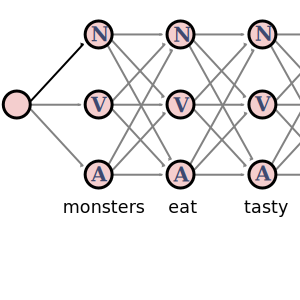
\includegraphics[width=1.5in]{figs/perc_dotprojection}}
  Given two vectors $\vec u$ and $\vec v$ their dot product $\dotp{\vec u}{\vec v}$ is $\sum_d u_d v_d$.
  The dot product grows large and positive when $\vec u$ and $\vec v$ point in same direction, grows
  %\begin{wrapfigure}{r}{2in}
  %  \vspace{-3em}
  %  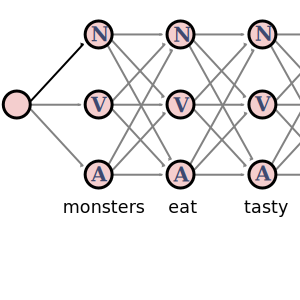
\includegraphics[width=2in]{figs/perc_dotprojection}.
  %\end{wrapfigure}
  large and negative when $\vec u$ and $\vec v$ point in opposite directions, and is zero when their are perpendicular.
  A useful geometric interpretation of dot products is \concept{projection}.
  Suppose $\norm{\vec u} = 1$, so that $\vec u$ is a \concept{unit vector}.
  We can think of any other vector $\vec v$ as consisting of two components: (a) a component in the direction of $\vec u$ and (b) a component that's perpendicular to $\vec u$.
  This is depicted geometrically to the right:
  Here, $\vec u = \langle 0.8, 0.6 \rangle$ and $\vec v = \langle 0.37, 0.73 \rangle$.
  We can think of $\vec v$ as the sum of two vectors, $\vec a$ and $\vec b$, where
  $\vec a$ is parallel to $\vec u$ and $\vec b$ is perpendicular.
  The length of $\vec b$ is exactly $\dotp{\vec u}{\vec v} = 0.734$, which is why you can think of
  dot products as projections: the dot product between $\vec u$ and $\vec v$ is the ``projection of $\vec v$ onto $\vec u$.''
%u=(0.8,0.6) --> (240,180) by *300
%v=(0.37,0.73) --> (110,220) by *300
\end{mathreview}

A question you should be asking yourself by now is: what does the
decision boundary of a perceptron look like?  You can actually answer
that question mathematically.  For a perceptron, the decision boundary
is precisely where the sign of the activation, $a$, changes from $-1$
to $+1$.  In other words, it is the set of points $\vx$ that achieve
\emph{zero} activation.  The points that are not clearly positive nor
negative.  For simplicity, we'll first consider the case where there
is no ``bias'' term (or, equivalently, the bias is zero).  Formally,
the decision boundary $\cB$ is:
\begin{equation}
\cB = \left\{ \vx ~:~ \sum_d w_d x_d = 0 \right\}
\end{equation}
We can now apply some linear algebra.  Recall that $\sum_d w_d x_d$ is
just the \concept{dot product} between the vector $\vw = \langle w_1,
w_2, \dots, w_D \rangle$ and the vector $\vx$.  We will write this as
$\dotp{\vw}{\vx}$.  Two vectors have a zero dot product if and only if
they are \concept{perpendicular}.  Thus, if we think of the weights as
a vector $\vw$, then the decision boundary is simply the plane
perpendicular to $\vw$.

\MoveNextFigure{-1cm}
\Figure{perc:geom}{picture of data points with hyperplane and weight vector}

This is shown pictorially in Figure~\ref{fig:perc:geom}.  Here, the
weight vector is shown, together with it's perpendicular plane.  This
plane forms the decision boundary between positive points and negative
points.  The vector points in the direction of the positive examples
and away from the negative examples.

One thing to notice is that the \emph{scale} of the weight vector is
irrelevant from the perspective of classification.  Suppose you take a
weight vector $\vw$ and replace it with $2 \vw$.  All activations are
now doubled.  But their sign does not change.  This makes complete
sense geometrically, since all that matters is which side of the plane
a test point falls on, now how far it is from that plane.  For this
reason, it is common to work with \koncept{normalized}{normalize}
weight vectors, $\vw$, that have length one; i.e., $\norm{\vw} = 1$.

\thinkaboutit{If I give you a non-zero weight vector $\vw$,
  how do I compute a weight vector $\vw'$ that points in the same
  direction but has a norm of one?}

\MoveNextFigure{-2cm}
\Figure{perc:proj}{The same picture as before, but with projections onto
  weight vector; then, below, those points along a
  one-dimensional axis with zero marked.}

The geometric intuition can help us even more when we realize that
dot products compute projections.  That is, the value $\dotp{\vw}{\vx}$
is just the distance of $\vx$ from the origin when projected
\emph{onto} the vector $\vw$.  This is shown in
Figure~\ref{fig:perc:proj}.  In that figure, all the data points are
projected onto $\vw$.  Below, we can think of this as a
one-dimensional version of the data, where each data point is placed
according to its projection along $\vw$.  This distance along $\vw$ is
exactly the \emph{activiation} of that example, with no bias.

From here, you can start thinking about the role of the bias term.
Previously, the threshold would be at zero.  Any example with a
negative projection onto $\vw$ would be classified negative; any
example with a positive projection, positive.  The bias simply moves
this threshold.  Now, after the projection is computed, $b$ is added
to get the overall activation.  The projection \emph{plus} $b$ is then
compared against zero.

\TODOFigure{perc:bias}{perceptron picture with bias}

Thus, from a geometric perspective, the role of the bias is to
\emph{shift} the decision boundary away from the origin, in the
direction of $\vw$.  It is shifted exactly $-b$ units.  So if $b$ is
positive, the boundary is shifted away from $\vw$ and if $b$ is
negative, the boundary is shifted toward $\vw$.  This is shown in
Figure~\ref{fig:perc:bias}.  This makes intuitive sense: a positive
bias means that more examples should be classified positive.  By
moving the decision boundary in the negative direction, more space
yields a positive classification.

The decision boundary for a perceptron is a very magical thing.  In
$D$ dimensional space, it is always a $D-1$-dimensional hyperplane.
(In two dimensions, a 1-d hyperplane is simply a line.  In three
dimensions, a 2-d hyperplane is like a sheet of paper.)  This
hyperplane divides space in half.  In the rest of this book, we'll
refer to the weight vector, and to hyperplane it defines,
interchangeably.

\Figure{perc:update}{perceptron picture with update, no bias}

The perceptron update can also be considered geometrically.  (For
simplicity, we will consider the \concept{unbiased} case.)  Consider
the situation in Figure~\ref{fig:perc:update}.  Here, we have a current
guess as to the hyperplane, and positive training example comes in
that is currently mis-classified.  The weights are updated: $\vw
\leftarrow \vw + y \vx$.  This yields the new weight vector, also
shown in the Figure.  In this case, the weight vector changed enough
that this training example is now correctly classified.

\section{Interpreting Perceptron Weights}

You may find yourself having run the perceptron, learned a really awesome classifier, and then wondering ``what the heck is this classifier doing?''
You might ask this question because you're curious to learn something about the underlying data.
You might ask this question because you want to make sure that the perceptron is learning ``the right thing.''
You might ask this question because you want to remove a bunch of features that aren't very useful because they're expensive to compute or take a lot of storage.

The perceptron learns a classifier of the form $\vx \mapsto \sign\left( \sum_d w_d x_d + b \right)$.
A reasonable question to ask is: how sensitive is the final classification to \emph{small changes} in some particular feature.
We can answer this question by taking a derivative.
If we arbitrarily take the $7$th feature we can compute $\frac \partial {\partial x_7} \left( \sum_d w_d x_d + b \right) = w_7$.
This says: the rate at which the activation changes as a function of the $7$th feature is exactly $w_7$.
This gives rise to a useful heuristic for interpreting perceptron weights:
\textbf{sort all the weights from largest (positive) to largest (negative), and take the top ten and bottom ten}.
The top ten are the features that the perceptron is most sensitive to for making positive predictions.
The bottom ten are the features that the perceptron is most sensitive to for making negative predictions.

This heuristic is useful, especially when the inputs $\vx$ consist entirely of binary values (like a bag of words representation).
The heuristic is less useful when the range of the individual features varies significantly.
The issue is that if you have one feat $x_5$ that's either $0$ or $1$, and another feature $x_7$ that's either $0$ or $100$, but $w_5 = w_7$, it's reasonable to say that $w_7$ is more important because it is likely to have a much larger influence on the final prediction.
The easiest way to compensate for this is simply to scale your features ahead of time:
this is another reason why feature scaling is a useful preprocessing step.


\section{Perceptron Convergence and Linear Separability}

You already have an intuitive feeling for why the perceptron works: it
moves the decision boundary in the direction of the training
examples.  A question you should be asking yourself is: does the
perceptron converge?  If so, what does it converge to?  And how long
does it take?

It is easy to construct data sets on which the perceptron algorithm
will never converge.  In fact, consider the (very uninteresting)
learning problem with \emph{no features}.  You have a data set
consisting of one positive example and one negative example.  Since
there are no features, the only thing the perceptron algorithm will
ever do is adjust the bias.  Given this data, you can run the
perceptron for a bajillion iterations and it will never settle down.
As long as the bias is non-negative, the negative example will cause
it to decrease.  As long as it is non-positive, the positive example
will cause it to increase.  Ad infinitum.  (Yes, this is a very
contrived example.)

\Figure{perc:separable}{separable data}

What does it mean for the perceptron to converge?  It means that it
can make an entire pass through the training data without making
\emph{any} more updates.  In other words, it has correctly classified
\emph{every} training example.  Geometrically, this means that it was
found some hyperplane that correctly segregates the data into positive
and negative examples, like that shown in
Figure~\ref{fig:perc:separable}.

\Figure{perc:inseparable}{inseparable data}

In this case, this data is \concept{linearly separable}.  This means
that there exists \emph{some} hyperplane that puts all the positive
examples on one side and all the negative examples on the other side.
If the training is \emph{not} linearly separable, like that shown in
Figure~\ref{fig:perc:inseparable}, then the perceptron has no hope of
converging.  It could never possibly classify each point correctly.

The somewhat surprising thing about the perceptron algorithm is that
\emph{if} the data is linearly separable, \emph{then} it will converge
to a weight vector that separates the data.  (And if the data is
inseparable, then it will never converge.)  This is great news.  It
means that the perceptron converges whenever it is even remotely
possible to converge.

The second question is: how long does it take to converge?  By ``how
long,'' what we really mean is ``how many updates?''  As is the case
for much learning theory, you will not be able to get an answer of the
form ``it will converge after $5293$ updates.''  This is asking too
much.  The sort of answer we can hope to get is of the form ``it will
converge after \emph{at most} $5293$ updates.''

What you might expect to see is that the perceptron will converge more
quickly for easy learning problems than for hard learning problems.
This certainly fits intuition.  The question is how to \emph{define}
``easy'' and ``hard'' in a meaningful way.  One way to make this
definition is through the notion of \concept{margin}.  If I give you a
data set and hyperplane that separates it% (like that shown in
%Figure~\ref{fig:perc:margin}) 
then the \emph{margin} is the distance
between the hyperplane and the nearest point.  Intuitively, problems
with large margins should be easy (there's lots of ``wiggle room'' to
find a separating hyperplane); and problems with small margins should
be hard (you really have to get a very specific well tuned weight
vector).

Formally, given a data set $\mat D$, a weight vector $\vw$ and bias
$b$, the margin of $\vw,b$ on $\mat D$ is defined as:
\begin{equation} \label{eq:margin}
\textit{margin}(\mat D, \vw, b)
= \brack{
     \min_{(\vx,y) \in \mat D} y \big( \dotp{\vw}{\vx} + b \big)
      & \text{if $\vw$ separates $\mat D$} \\
    -\infty & \text{otherwise}
}
\end{equation}
In words, the margin is only defined if $\vw,b$ actually separate the
data (otherwise it is just $-\infty$).  In the case that it separates
the data, we find the point with the minimum activation, after the
activation is multiplied by the label.
\thinkaboutit{So long as the margin is not $-\infty$, it is always
  positive.  Geometrically this makes sense, but why does
  Eq~\eqref{eq:margin} yield this?}

For some historical reason (that is unknown to the author), margins
are always denoted by the Greek letter $\gamma$ (gamma).  One often
talks about the \concept{margin of a data set}.  The margin of a data
set is the largest attainable margin on this data.  Formally:
\begin{equation} \label{eq:margin2}
\textit{margin}(\mat D)
= 
\sup_{\vw,b} \textit{margin}(\mat D, \vw, b)
\end{equation}
In words, to compute the margin of a data set, you ``try'' every
possible $\vw,b$ pair.  For each pair, you compute its margin.  We
then take the largest of these as the overall margin of the
data.\sidenote{You can read ``$\sup$'' as ``$\max$'' if you like: the
  only difference is a technical difference in how the $-\infty$ case
  is handled.}  If the data is not linearly separable, then the value
of the $\sup$, and therefore the value of the margin, is $-\infty$.

There is a famous theorem due to
Rosenblatt\mycite{rosenblatt58perceptron} that shows that the number
of errors that the perceptron algorithm makes is bounded by
$\ga^{-2}$.  More formally:

\begin{theorem}[Perceptron Convergence Theorem] \label{thm:perc:perc}
  Suppose the perceptron algorithm is run on a linearly separable data
  set $\mat D$ with margin $\ga > 0$.  Assume that $\norm{\vx} \leq 1$
  for all $\vx \in \mat D$.  Then the algorithm will converge after at
  most $\frac 1 {\ga^2}$ updates.
\end{theorem}

The proof of this theorem is elementary, in the sense that it does not
use any fancy tricks: it's all just algebra.  The \emph{idea} behind
the proof is as follows.  If the data is linearly separable with
margin $\ga$, then there exists some weight vector $\vw^*$ that
achieves this margin.  Obviously we don't know what $\vw^*$ is, but we
know it exists.  The perceptron algorithm is trying to find a weight
vector $\vw$ that points roughly in the same direction as $\vw^*$.
(For large $\ga$, ``roughly'' can be very rough.  For small $\ga$,
``roughly'' is quite precise.)  Every time the perceptron makes an
update, the angle between $\vw$ and $\vw^*$ changes.  What we prove is
that the angle actually \emph{decreases.}  We show this in two steps.
First, the dot product $\dotp{\vw}{\vw^*}$ increases a lot.  Second,
the norm $\norm{\vw}$ does not increase very much.  Since the dot
product is increasing, but $\vw$ isn't getting too long, the angle
between them has to be shrinking.  The rest is algebra.

\begin{myproof}{\ref{thm:perc:perc}}
  The margin $\ga > 0$ must be realized by some set of parameters, say
  $\vx^*$.  Suppose we train a perceptron on this data.  Denote by
  $\vw\zth$ the initial weight vector, $\vw\oth$ the weight vector
  after the \emph{first update}, and $\vw\kth$ the weight vector after
  the $k$th update.  (We are essentially ignoring data points on which
  the perceptron doesn't update itself.)  First, we will show that
  $\dotp{\vw^*}{\vw\kth}$ grows quicky as a function of $k$.  Second,
  we will show that $\norm{\vw\kth}$ does not grow quickly.

  First, suppose that the $k$th update happens on example $(\vx,y)$.
  We are trying to show that $\vw\kth$ is becoming aligned with
  $\vw^*$.  Because we updated, know that this example was
  misclassified: $y \dotp{\vw\kpth}{\vx} < 0$.  After the update, we get
  $\vw\kth = \vw\kpth + y \vx$.  We do a little computation:
  \begin{align}
    \dotp{\vw^*}{\vw\kth}
    &= \dotp{\vw^*}{\left(\vw\kpth + y \vx\right)} 
         \becauseof{definition of $\vw\kth$}
    \\
    &= \dotp{\vw^*}{\vw\kpth} + y \dotp{\vw^*}{\vx}
         \becauseof{vector algebra}
    \\
    &\geq \dotp{\vw^*}{\vw\kpth} + \ga
         \becauseof{$\vw^*$ has margin $\ga$}
  \end{align}
  Thus, every time $\vw\kth$ is updated, its projection onto $\vw^*$
  increases by at least $\ga$.  \textcolor{darkblue}{Therefore:
    $\dotp{\vw^*}{\vw\kth} \geq k \ga$.}

  Next, we need to show that the increase of $\ga$ along $\vw^*$
  occurs because $\vw\kth$ is getting closer to $\vw^*$, not just
  because it's getting exceptionally long.  To do this, we compute the
  norm of $\vw\kth$:
  \begin{align}
    & \norm{\vw\kth}^2 \nonumber\\
    &= \norm{\vw\kpth + y \vx}^2
         \becauseof{def. of $\vw\kth$} \\
    &= \norm{\vw\kpth}^2 + y^2 \norm{\vx}^2 + 2 y \dotp{\vw\kpth}{\vx}
         \becauseof{quadratic rule} \\
    &\leq \norm{\vw\kpth}^2 + 1 + 0
         \becauseof{assumption and $a < 0$}
  \end{align}
  Thus, the squared norm of $\vw\kth$ increases by at most one every
  update.  \textcolor{darkblue}{Therefore: $\norm{\vw\kth}^2 \leq k$.}

  Now we put together the two things we have learned before.  By our
  first conclusion, we know $\dotp{\vw^*}{\vw\kth} \geq k \ga$.  But
  our second conclusion, $\sqrt{k} \geq \norm{\vw\kth}^2$.  Finally,
  because $\vw^*$ is a unit vector, we know that $\norm{\vw\kth} \geq
  \dotp{\vw^*}{\vw\kth}$.  Putting this together, we have:
  \begin{equation}
    \sqrt k 
    \quad\geq\quad
    \norm{\vw\kth}
    \quad\geq\quad
    \dotp{\vw^*}{\vw\kth}
    \quad\geq\quad
    k\ga
  \end{equation}
  Taking the left-most and right-most terms, we get that $\sqrt{k}
  \geq k \ga$.  Dividing both sides by $k$, we get $\frac 1 {\sqrt{k}}
  \geq \ga$ and therefore $k \leq \frac 1 {\ga^2}$.  This means
  that once we've made $\frac 1 {\ga^2}$ updates, we cannot make
  any more!
\end{myproof}

\thinkaboutit{Perhaps we don't want to assume that all $\vx$ have norm
  at most $1$.  If they have all have norm at most $R$, you can
  achieve a very similar bound.  Modify the perceptron convergence
  proof to handle this case.}


It is important to keep in mind what this proof shows and what it does
not show.  It shows that if I give the perceptron data that is
linearly separable with margin $\gamma > 0$, then the perceptron will
converge to a solution that separates the data.  And it will converge
quickly when $\gamma$ is large.  It does not say anything about the
solution, \emph{other than} the fact that it separates the data.  In
particular, the proof makes use of the maximum margin separator.  But
the perceptron is not guaranteed to \emph{find} this maximum margin
separator.  The data may be separable with margin $0.9$ and the
perceptron might still find a separating hyperplane with a margin of
only $0.000001$.  Later (in Chapter~\ref{sec:loss}), we will see
algorithms that explicitly try to find the maximum margin solution.

\thinkaboutit{Why does the perceptron convergence bound not contradict
  the earlier claim that poorly ordered data points (e.g., all
  positives followed by all negatives) will cause the perceptron to
  take an astronomically long time to learn?}

\section{Improved Generalization: Voting and Averaging}

In the beginning of this chapter, there was a comment that the
perceptron works amazingly well.  This was a half-truth.  The
``vanilla'' perceptron algorithm does well, but not \emph{amazingly}
well.  In order to make it more competitive with other learning
algorithms, you need to modify it a bit to get better generalization.
The key issue with the vanilla perceptron is that \emph{it counts
  later points more than it counts earlier points}.

To see why, consider a data set with $10,000$ examples.  Suppose that
after the first $100$ examples, the perceptron has learned a really
good classifier.  It's so good that it goes over the next $9899$
examples without making \emph{any} updates.  It reaches the $10,000$th
example and makes an error.  It updates.  For all we know, the update
on this $10,000$th example \emph{completely ruins} the weight vector
that has done so well on $99.99\%$ of the data!

What we would like is for weight vectors that ``survive'' a long time
to get more say than weight vectors that are overthrown quickly.  One
way to achieve this is by \concept{voting}.  As the perceptron learns,
it remembers how long each hyperplane survives.  At test time, each
hyperplane encountered during training ``votes'' on the class of a
test example.  If a particular hyperplane survived for $20$ examples,
then it gets a vote of $20$.  If it only survived for one example, it
only gets a vote of $1$.  In particular, let $(\vw,b)\oth, \dots,
(\vw,b)\Kth$ be the $K+1$ weight vectors encountered during training,
and $c\oth, \dots, c\Kth$ be the survival times for each of these
weight vectors.  (A weight vector that gets immediately updated gets
$c=1$; one that survives another round gets $c=2$ and so on.)  Then
the prediction on a test point is:
\begin{equation} \label{eq:perc:vote}
  \hat y = \sign \left(
    \sum_{k=1}^K c\kth 
      \sign \left(
        \dotp{\vw\kth}{\hat\vx} + b\kth
        \right)
      \right)
\end{equation}
This algorithm, known as the \concept{voted perceptron} works quite
well in practice, and there is some nice theory showing that it is
guaranteed to generalize better than the vanilla perceptron.
Unfortunately, it is also completely impractical.  If there are $1000$
updates made during perceptron learning, the voted perceptron requires
that you store $1000$ weight vectors, together with their counts.
This requires an absurd amount of storage, and makes prediction $1000$
times slower than the vanilla perceptron.

\thinkaboutit{The \emph{training algorithm} for the voted perceptron
  is the same as the vanilla perceptron.  In particular, in line 5 of
  Algorithm~\ref{alg:perc:perc}, the activation on a training example
  is computed based on the \emph{current weight vector}, not based on
  the voted prediction.  Why?}

A much more practical alternative is the \concept{averaged
  perceptron}.  The idea is similar: you maintain a collection of
weight vectors and survival times.  However, at test time, you predict
according to the \emph{average} weight vector, rather than the
voting.  In particular, the prediction is:
\begin{equation} \label{eq:perc:avg}
  \hat y = \sign \left(
    \sum_{k=1}^K c\kth 
      \left(
        \dotp{\vw\kth}{\hat\vx} + b\kth
        \right)
      \right)
\end{equation}
The only difference between the voted prediction,
Eq~\eqref{eq:perc:vote}, and the averaged prediction,
Eq~\eqref{eq:perc:avg}, is the presense of the interior $\sign$
operator.  With a little bit of algebra, we can rewrite the test-time
prediction as:
\begin{equation}
  \hat y = \sign \left(
    \dotp{\textcolor{darkblue}{\left(
        \sum_{k=1}^K c\kth \vw\kth 
        \right)}}{\hat\vx} +
      \textcolor{darkred}{\sum_{k=1}^K c\kth b\kth}
      \right)
\end{equation}
The advantage of the averaged perceptron is that we can simply
maintain a \emph{running sum} of the averaged weight vector (the blue
term) and averaged bias (the red term).  Test-time prediction is then
just as efficient as it is with the vanilla perceptron.

\newalgorithm%
  {perc:avgperc}%
  {\FUN{AveragedPerceptronTrain}(\VAR{$\mat D$}, \VAR{MaxIter})}
  {
\SETST{$\vw$}{$\langle \CON{0}, \CON{0}, \dots \CON{0} \rangle$
  \quad,\quad
  \VAR{$b$} $\leftarrow$ \CON{0}}
  \COMMENT{initialize weights and bias}
\SETST{$\vec u$}{$\langle \CON{0}, \CON{0}, \dots \CON{0} \rangle$
  \quad,\quad
  \VAR{$\beta$} $\leftarrow$ \CON{0}}
  \COMMENT{initialize cached weights and bias}
\SETST{c}{\CON{1}}
  \COMMENT{initialize example counter to one}
\FOR{\VAR{iter} = \CON{1} \dots \VAR{MaxIter}}
\FORALL{(\VAR{$\vx$},\VAR{$y$}) $\in$ \VAR{$\mat D$}}
\IF{\VAR{$y$}$\left( \dotp{\VARm{\vw}}{\VARm{\vx}} + \VARm{b} \right) \leq \CON{0}$}
\SETST{$\vw$}{\VAR{$\vw$} + \VAR{$y$} \VAR{$\vx$}}
  \COMMENT{update weights}
\SETST{$b$}{\VAR{$b$} + \VAR{$y$}}
  \COMMENT{update bias}
\SETST{$\vec u$}{\VAR{$\vec u$} + \VAR{$y$} \VAR{c} \VAR{$\vx$}}
  \COMMENT{update cached weights}
\SETST{$\beta$}{\VAR{$\beta$} + \VAR{$y$} \VAR{c}}
  \COMMENT{update cached bias}
\ENDIF
\SETST{c}{\VAR{c} + \CON{1}}
  \COMMENT{increment counter regardless of update}
\ENDFOR
\ENDFOR
\RETURN \VAR{$\vw$} - $\frac 1 {\VAR{c}}$ \VAR{$\vec u$}, 
        \VAR{$b$}   - $\frac 1 {\VAR{c}}$ \VAR{$\beta$}
\COMMENT{return averaged weights and bias}
}

The full training algorithm for the averaged perceptron is shown in
Algorithm~\ref{alg:perc:avgperc}.  Some of the notation is changed
from the original perceptron: namely, vector operations are written as
vector operations, and the activation computation is folded into the
error checking.

It is probably not immediately apparent from
Algorithm~\ref{alg:perc:avgperc} that the computation unfolding is
precisely the calculation of the averaged weights and bias.  The most
\emph{natural} implementation would be to keep track of an averaged
weight vector $\vec u$.  At the end of every example, you would
increase $\vec u \leftarrow \vec u + \vw$ (and similarly for the
bias).  However, such an implementation would require that you updated
the averaged vector on \emph{every} example, rather than just on the
examples that were incorrectly classified!  Since we hope that
eventually the perceptron learns to do a good job, we would hope that
it will not make updates on every example.  So, ideally, you would
like to only update the averaged weight vector when the actual weight
vector changes.  The slightly clever computation in
Algorithm~\ref{alg:perc:avgperc} achieves this.

\thinkaboutit{By writing out the computation of the averaged weights
  from Eq~\eqref{eq:perc:avg} as a telescoping sum, derive the
  computation from Algorithm~\ref{alg:perc:avgperc}.}

%\TODOFigure{perc:avgperc}{train/test performance of vanilla versus
%  averaged perceptron to show early stopping}

The averaged perceptron is almost always better than the perceptron,
in the sense that it generalizes better to test data.  However, that
does not free you from having to do \concept{early stopping}.  It
will, eventually, overfit.  
%Figure~\ref{fig:perc:avgperc} shows the
%performance of the vanilla perceptron and the averaged perceptron on
%the same data set, with both training and test performance.  As you
%can see, the averaged perceptron \emph{does} generalize better.  But
%it also does begin to overfit eventually.

\section{Limitations of the Perceptron}


Although the perceptron is very useful, it is fundamentally limited in
a way that neither decision trees nor KNN are.  Its limitation is that
its decision boundaries can \emph{only} be linear.  The classic way of
showing this limitation is through the XOR problem (XOR = exclusive
or).  The XOR problem is shown graphically in
Figure~\ref{fig:perc:xor}.  It consists of four data points, each at a
corner of the unit square.  The labels for these points are the same,
along the diagonals.  You can try, but you will not be able to find a
linear decision boundary that perfectly separates these data points.

\Figure{perc:xor}{picture of xor problem}

One question you might ask is: do XOR-like problems exist in the real
world?  Unfortunately for the perceptron, the answer is yes.  Consider
a sentiment classification problem that has three features that simply
say whether a given word is contained in a review of a course.  These
features are: \feat{excellent}, \feat{terrible} and \feat{not}.  The
\feat{excellent} feature is indicative of positive reviews and the
\feat{terrible} feature is indicative of negative reviews.  But in the
presence of the \feat{not} feature, this categorization flips.

One way to address this problem is by adding \concept{feature
  combinations}.  We could add two additional features:
\feat{excellent-and-not} and \feat{terrible-and-not} that indicate
a conjunction of these base features.  By assigning weights as
follows, you can achieve the desired effect:
\begin{align*}
w_{\feat{execellent}} &= +1
& w_{\feat{terrible}} &= -1
& w_{\feat{not}} &= 0 \\
w_{\feat{execllent-and-not}} &= -2 
& w_{\feat{terrible-and-not}} &= +2
\end{align*}
In this particular case, we have addressed the problem.  However, if
we start with $D$-many features, if we want to add all pairs, we'll
blow up to ${D \choose 2} = \cO(D^2)$ features through this
\concept{feature mapping}.  And there's no guarantee that pairs of
features is enough.  We might need triples of features, and now we're
up to ${D \choose 3} = \cO(D^2)$ features.  These additional features
will drastically increase computation and will often result in a
stronger propensity to overfitting.

\thinkaboutit{Suppose that you took the XOR problem and added one new
  feature: $x_3 = x_1 \land x_2$ (the logical and of the two existing
  features).  Write out feature weights and a bias that would achieve
  perfect classification on this data.}

In fact, the ``XOR problem'' is so significant that it basically
killed research in classifiers with linear decision boundaries for a
decade or two.  Later in this book, we will see two alternative
approaches to taking key ideas from the perceptron and generating
classifiers with non-linear decision boundaries.  One approach is to
combine multiple perceptrons in a single framework: this is the
\concept{neural networks} approach (see Chapter~\ref{sec:nnet}).  The
second approach is to find computationally efficient ways of doing
feature mapping in a computationally and statistically efficient way:
this is the \concept{kernels} approach (see Chapter~\ref{sec:kernel}).

% \TODOFigure{perc:mapping}{mapping two dimensional data, three points,
%   into five dimensional data}

% In addition to the perceptron not being able to \emph{solve} problems
% that require non-linear decision boundaries, it will not even
% \emph{converge} on such problems.  However, there is a simple data
% transformation that ensures linear separability.  Suppose you start
% $N$ training examples in $D$ dimensions.  You will end up with $N$
% training examples in $D+N$ dimensions.  When we map data point $\vx_n
% \mapsto \vx'_n$, you will \emph{copy} the first $D$ dimensions.  After
% those original $D$ dimension, you place an \emph{indicator} in the
% $D+n$th position and zeros everywhere else.
% Figure~\ref{fig:perc:mapping} shows an example on a very small
% training set.

% \thinkaboutit{Completely ignoring the first $D$ many features,
%   construct a weight vector that achieves perfect classification on
%   this data.}

% In practice, there is little reason to \emph{actually} perform this
% mapping.  It is more interesting from a theoretical perspective.  

\section{Further Reading}

TODO further reading


\begin{comment}
   -``Neural network'' interpretation
   - Update rule
   - Linear decision boundaries
   - Connection to geometry, linear algebra, dot products, etc.
   - Linear separability and the XOR problem
   - Margins
   - Convergence
\end{comment}


%%% Local Variables: 
%%% mode: latex
%%% TeX-master: "courseml"
%%% End: 


%\chapter{Practical Issues} \label{sec:prac}

%start at 3 end at 14; left is -0.8 right is 15.4
%\begin{textblock}{1}(15.4,\chapterlabel)\tikz\node [fill=darkergreen,text=white,draw,circle] (chnode) {\normalfont\sffamily\Huge\bfseries\scshape \chapterlabel~~~};\end{textblock}
%\begin{textblock}{1}(-0.8,14)\tikz\node [fill=darkergreen,text=white,draw,circle] (chnode) {\normalfont\sffamily\Huge\bfseries\scshape ~~~\chapterlabel};\end{textblock}

\chapterquote{A ship in port is safe, but that is not what ships are for.}{Grace~Hopper}

\begin{learningobjectives}
\item Translate between a problem description and a concrete learning
  problem.
\item Perform basic feature engineering on image and text data.
\item Explain how to use cross-validation to tune hyperparameters and
  estimate future performance.
\item Compare and contrast the differences between several evaluation
  metrics.
\item Explain why feature combinations are important for learning with
  some models but not others.
\item Explain the relationship between the three learning techniques
  you have seen so far.
\item Apply several debugging techniques to learning algorithms.
\end{learningobjectives}

\dependencies{\chref{sec:dt},\chref{sec:knn},\chref{sec:perc}}

\newthought{At this point,} you have seen three qualitatively
different models for learning: decision trees, nearest neighbors, and
perceptrons.  You have also learned about clustering with the
$K$-means algorithm.  You will shortly learn about more complex
models, most of which are variants on things you already know.
However, before attempting to understand more complex models of
learning, it is important to have a firm grasp on how to use machine
learning in practice.  This chapter is all about how to go from an
abstract learning problem to a concrete implementation.  You will see
some examples of ``best practices'' along with justifications of these
practices.

In many ways, going from an abstract problem to a concrete learning
task is more of an art than a science.  However, this art can have a
huge impact on the practical performance of learning systems.  In many
cases, moving to a more complicated learning algorithm will gain you a
few percent improvement.  Going to a better representation will gain
you an order of magnitude improvement.  To this end, we will discuss
several high level ideas to help you develop a better artistic
sensibility.

\section{The Importance of Good Features}

Machine learning is magical.  You give it data and it manages to
classify that data.  For many, it can actually outperform a human!
But, like so many problems in the world, there is a significant
``garbage in, garbage out'' aspect to machine learning.  If the data
you give it is trash, the learning algorithm is unlikely to be able to
overcome it.

Consider a problem of object recognition from images.  If you start
with a $100 \times 100$ pixel image, a very easy feature
representation of this image is as a $30,000$ dimensional vector,
where each dimension corresponds to the red, green or blue component
of some pixel in the image.  So perhaps feature 1 is the amount of red
in pixel $(1,1)$; feature 2 is the amount of green in that pixel; and
so on.  This is the \concept{pixel representation} of images.

\Figure{prac_imagepix}{object recognition in pixels}

One thing to keep in mind is that the pixel representation
\emph{throws away} all locality information in the image.  Learning
algorithms don't care about features: they only care about feature
values.  So I can \emph{permute} all of the features, with no effect
on the learning algorithm (so long as I apply the same permutation to
all training and test examples).  Figure~\ref{fig:prac_imagepix} shows
some images whose pixels have been randomly permuted (in this case only
the pixels are permuted, not the colors).  All of these objects are
things that you've seen plenty of examples of; can you identify them?
Should you expect a machine to be able to?

\Figure{prac_imagepatch}{object recognition in patches}
\Figure{prac_imageshape}{object recognition in shapes}

An alternative representation of images is the \concept{patch
  representation}, where the unit of interest is a small rectangular
block of an image, rather than a single pixel.  Again, permuting the
patches has no effect on the classifier.
Figure~\ref{fig:prac_imagepatch} shows the same images in patch
representation.  Can you identify them?  A final representation is a
\concept{shape representation}.  Here, we throw out all color and
pixel information and simply provide a bounding polygon.
Figure~\ref{fig:prac_imageshape} shows the same images in this
representation.  Is this now enough to identify them?  (If not, you
can find the answers in Figure~\ref{fig:prac_imageimage} at the end of the chapter.)


\Table{prac:bow}{Bag of (most frequent) words representation for the Decision Tree and KNN chapters of this book, after dropping high frequency words like ``the''.}{@{}p{2cm}@{}p{2cm}@{}}{
    \hline
data ~ learning ~ training ~ set ~ predict ~ feature ~ function ~ test ~ machine ~ loss ~ alice ~ tree ~ guess ~ features ~ algorithm &
data ~ knn ~ dimensions ~ points ~ feature ~ figure ~ decision ~ features ~ point ~ fig ~ training ~ set ~ space ~ examples \\
\hline
}


    
\TODOFigure{prac:bow}{BOW repr of one positive and one negative review}

In the context of \concept{text categorization} (for instance, the
sentiment recognition task), one standard representation is the
\concept{bag of words} representation.  Here, we have one feature for
each unique word that appears in a document.  For the feature
\feat{happy}, the feature value is the number of times that the word
``happy'' appears in the document.  The bag of words (BOW)
representation throws away all position information.
Table~\ref{tab:prac:bow} shows a BOW representation for two chapters of this book.
Can you tell which is
which?

\section{Irrelevant and Redundant Features}

One big difference between learning models is how robust they are to
the addition of noisy or irrelevant features.  Intuitively, an
irrelevant feature is one that is completely uncorrelated with the
prediction task.  A feature $f$ whose expectation does not depend on
the label $\Ep[f \| Y] = \Ep[f]$ might be irrelevant.  For instance,
the presence of the word ``the'' might be largely irrelevant for
predicting whether a course review is positive or negative.  

A secondary issue is how well these algorithms deal with
\concept{redundant features}.  Two features are redundant if they are
highly correlated, regardless of whether they are correlated with the
task or not.  For example, having a bright red pixel in an image at
position $(20,93)$ is probably highly redundant with having a bright
red pixel at position $(21,93)$.  Both might be useful (e.g., for
identifying fire hydrants), but because of how images are structured,
these two features are likely to co-occur frequently.

\thinkaboutit{Is it possible to have a feature $f$ whose expectation
  does not depend on the label, but is nevertheless still useful for
  prediction?}


When thinking about robustness to irrelevant or redundant features, it
is usually not worthwhile thinking of the case where one has $999$
great features and $1$ bad feature.  The interesting case is when the
bad features outnumber the good features, and often outnumber by a
large degree.  %For instance, perhaps the number of good features is
%something like $\log D$ out of a set of $D$ total features.  
The
question is how robust are algorithms in this case.\sidenote{You might
  think it's absurd to have so many irrelevant features, but the cases
  you've seen so far (bag of words, bag of pixels) are both reasonable
  examples of this!  How many words, out of the entire English
  vocabulary (roughly $10,000-100,000$ words), are actually useful for
  predicting positive and negative course reviews?}

For shallow \concept{decision trees}, the model explicitly selects
features that are highly correlated with the label.  In particular, by
limiting the depth of the decision tree, one can at least \emph{hope}
that the model will be able to throw away irrelevant features.
Redundant features are almost certainly thrown out: once you select
one feature, the second feature now looks mostly useless.  The only
possible issue with irrelevant features is that even though they're
irrelevant, they \emph{happen to} correlate with the class label on
the training data, but chance.

As a thought experiment, suppose that we have $N$ training examples,
and exactly half are positive examples and half are negative
examples.  Suppose there's some binary feature, $f$, that is completely
uncorrelated with the label.  This feature has a 50/50 chance of
appearing in any example, regardless of the label.  In principle, the
decision tree should \emph{not} select this feature.  But, by chance,
especially if $N$ is small, the feature might \emph{look} correlated
with the label.  This is analogous to flipping two coins
simultaneously $N$ times.  Even though the coins are independent, it's
entirely possible that you will observe a sequence like $(H,H), (T,T),
(H,H), (H,H)$, which makes them look entirely correlated!  The hope is
that as $N$ grows, this becomes less and less likely.  In fact, we can
explicitly compute how likely this is to happen.

To do this, let's fix the sequence of $N$ labels.  We now flip a coin
$N$ times and consider how likely it is that it exactly matches the
label.  This is easy: the probability is $0.5^N$.  Now, we would also
be confused if it exactly matched \emph{not} the label, which has the
same probability.  So the chance that it looks perfectly correlated is
$0.5^N + 0.5^N = 0.5^{N-1}$.  Thankfully, this shrinks down very small
(e.g., $10^{-6}$) after only $21$ data points, meaning that even with a very small training set, the chance that a random feature \emph{happens} to correlate exactly with the label is tiny.

This makes us happy.  The problem is that we don't have one irrelevant
feature: we have many! If we randomly pick
two irrelevant features, each has the same probability of
perfectly correlating: $0.5^{N-1}$.  But since there are two and
they're independent coins, the chance that \emph{either} correlates
perfectly is $2 \times 0.5^{N-1} = 0.5^{N-2}$.  In general, if we have
$K$ irrelevant features, all of which are random independent coins,
the chance that at least one of them perfectly correlates is
$0.5^{N-K}$.  This suggests that if we have a sizeable number $K$ of
irrelevant features, we'd better have at \emph{least} $K+21$ training
examples.

Unfortunately, the situation is actually worse than this.  In the
above analysis we only considered the case of \emph{perfect}
correlation.  We could also consider the case of \emph{partial}
correlation, which would yield even higher probabilities.  
Suffice it to say that even
decision trees can become confused.

\TODOFigure{prac:addirrel}{data from high dimensional warning, interpolated}

In the case of \concept{$K$-nearest neighbors}, the situation is
perhaps more dire.  Since KNN weighs each feature just as much as
another feature, the introduction of irrelevant features can
completely mess up KNN prediction.  In fact, as you saw, in high
dimensional space, randomly distributed points all look approximately
the same distance apart.  If we add lots and lots of randomly
distributed features to a data set, then all distances still
converge.
%  This is shown experimentally in
%Figure~\ref{fig:prac:addirrel}, where we start with the digit
%categorization data and continually add irrelevant, uniformly
%distributed features, and generate a histogram of distances.
%Eventually, all distances converge.

In the case of the \concept{perceptron}, one can \emph{hope} that it
might learn to assign zero weight to irrelevant features.  For
instance, consider a binary feature is randomly one or zero
independent of the label.  If the perceptron makes just as many
updates for positive examples as for negative examples, there is a
reasonable chance this feature weight will be zero.  At the very
least, it should be small.

\thinkaboutit{What happens with the perceptron with truly redundant
  features (i.e., one is literally a copy of the other)?}


\section{Feature Pruning and Normalization}

In text categorization problems, some words simply do not appear very
often.  Perhaps the word ``groovy''\sidenote{This is typically
  positive indicator, or at least it was back in the US in the 1970s.}
appears in exactly one training document, which is positive.  Is it
really worth keeping this word around as a feature?  It's a dangerous
endeavor because it's hard to tell with just one training example if
it is really correlated with the positive class, or is it just noise.
You could hope that your learning algorithm is smart enough to figure
it out.  Or you could just remove it.  That means that (a) the
learning algorithm won't have to figure it out, and (b) you've reduced
the number of dimensions you have, so things should be more efficient,
and less ``scary.''

\TODOFigure{prac:pruning}{effect of pruning on text data}

This idea of feature pruning is very useful and applied in many
applications.  It is easiest in the case of binary features.  If a
binary feature only appears some small number $K$ times (in the
training data: no fair looking at the test data!), you simply remove
it from consideration.  (You might also want to remove features that
appear in all-but-$K$ many documents, for instance the word ``the''
appears in pretty much every English document ever written.)  Typical
choices for $K$ are $1, 2, 5, 10, 20, 50$, mostly depending on the
size of the data.  On a text data set with $1000$ documents, a cutoff
of $5$ is probably reasonable.  On a text data set the size of the
web, a cut of $50$ or even $100$ or $200$ is probably
reasonable\sidenote{According to Google, the following words (among
  many others) appear $200$ times on the web: moudlings, agaggagctg,
  setgravity, rogov, prosomeric, spunlaid, piyushtwok, telelesson,
  nesmysl, brighnasa.  For comparison, the word ``the'' appears
  $19,401,194,714$ (19 billion) times.}.
Figure~\ref{fig:prac:pruning} shows the effect of pruning on a
sentiment analysis task.  In the beginning, pruning does not hurt (and
sometimes helps!) but eventually we prune away all the interesting
words and performance suffers.

\begin{mathreview}{Data Statistics: Means and Variances}
  We often need to discuss various statistics of a data set.
  Most often, it is enough to consider univariate (one-dimensional) data.
  Suppose we have $N$ real valued numbers $z_1, z_2, \dots, z_N$.
  The \concept{sample mean} (or just \concept{mean}) of these numbers is just their average value, or expected value: $\mu = \frac 1 N \sum_n z_n$.
  The \concept{sample variance} (or just \concept{variance}) measures how much they vary around their mean: $\si^2 = \frac 1 {N-1} \sum_n (z_n - \mu)^2$, where $\mu$ is the sample mean.
  
~\\

  The mean and variance have convenient interpretations in terms of prediction.
  Suppose we wanted to choose a single constant value to ``predict'' the next $z$, and were minimizing squared error.
  Call this constant value $a$.
  Then $a = \argmin_{a \in \R} \frac 1 2 \sum_n (a - z_n)^2$. 
  (Here, the $\frac 1 2$ is for convenience and does not change the answer.)
  To solve for $a$, we can take derivatives and set to zero:
    $\frac \partial {\partial a} \frac 1 2 \sum_n (a - z_n)^2
     = \sum_n (a - z_n) = N a - \sum_n z_n$; therefore $N a = \sum_n z_n$ and $a = \mu$.
  This means that the sample mean is the number that minimizes squared error to the sample.
  Moreover, the variance is propotional to the squared error of that ``predictor.''
\end{mathreview}

\TODOFigure{prac:variance}{effect of pruning on vision}

In the case of real-valued features, the question is how to extend the
idea of ``does not occur much'' to real values.  A reasonable
definition is to look for features with \emph{low variance}.  In fact,
for binary features, ones that almost never appear or almost always
appear will also have low variance.  Figure~\ref{fig:prac:variance}
shows the result of pruning low-variance features on the digit
recognition task.  Again, at first pruning does not hurt (and
sometimes helps!) but eventually we have thrown out all the useful
features.

\thinkaboutit{Earlier we discussed the problem of \emph{scale} of
  features (e.g., millimeters versus centimeters).  Does this have an
  impact on variance-based feature pruning?}

It is often useful to \concept{normalize} the data so that it is
consistent in some way.  There are two basic types of normalization:
\concept{feature normalization} and \concept{example normalization}.
In feature normalization, you go through each feature and adjust it
the same way across all examples.  In example normalization, each
example is adjusted individually.

\TODOFigure{prac:transform}{picture of centering, scaling by variance and scaling by absolute value}

The goal of both types of normalization is to make it \emph{easier}
for your learning algorithm to learn.  In feature normalization, there
are two standard things to do:
\begin{enumerate}
\item Centering: moving the entire data set so that it is centered
  around the origin.
\item Scaling: rescaling each feature so that one of the following
  holds:
\begin{enumerate}
\item Each feature has variance $1$ across the training data.
\item Each feature has maximum absolute value $1$ across the training
  data.
\end{enumerate}
\end{enumerate}
These transformations are shown geometrically in
Figure~\ref{fig:prac:transform}.  The goal of centering is to make
sure that no features are arbitrarily large.  The goal of scaling is
to make sure that all features have roughly the same scale (to avoid
the issue of centimeters versus millimeters).

\thinkaboutit{For the three models you know about (KNN, DT,
  Perceptron), which are most sensitive to centering?  Which are most
  sensitive to scaling?}

These computations are fairly straightforward.  Here, $x_{n,d}$ refers
to the $d$th feature of example $n$.  Since it is very rare to apply
scaling without previously applying centering, the expressions below
for scaling assume that the data is already centered.
\begin{align}
\text{Centering:} && x_{n,d} &\leftarrow x_{n,d} - \mu_d \\
\text{Variance Scaling:} && x_{n,d} &\leftarrow x_{n,d} / \si_d \\
\text{Absolute Scaling:} && x_{n,d} &\leftarrow x_{n,d} / r_d \\
&\textit{where:}
& \mu_d &= \frac 1 N \sum_n x_{n,d} \\
&& \si_d &= \sqrt{ \frac 1 {N-1} \sum_n (x_{n,d} - \mu_d)^2 } \\
&& r_d   &= \max_n \ab{x_{n,d}}
\end{align}


In practice, if the dynamic range of your features is already some
subset of $[-2,2]$ or $[-3,3]$, then it is probably not worth the
effort of centering and scaling.  (It's an effort because you have to
keep around your centering and scaling calculations so that you can
apply them to the test data as well!)  However, if some of your
features are orders of magnitude larger than others, it might be
helpful.  Remember that you might know best: if the difference in
scale is actually significant for your problem, then rescaling might
throw away useful information.

One thing to be wary of is centering binary data.  In many cases,
binary data is very \emph{sparse}: for a given example, only a few of
the features are ``on.''  For instance, out of a vocabulary of
$10,000$ or $100,000$ words, a given document probably only contains
about $100$.  From a storage and computation perspective, this is very
useful.  However, after centering, the data will no longer be sparse and
you will pay dearly with outrageously slow implementations.

\TODOFigure{prac:exnorm}{example of example normalization}

In \concept{example normalization}, you view examples one at a time.
The most standard normalization is to ensure that the length of each
example vector is one: namely, each example lies somewhere on the unit
hypersphere.  This is a simple transformation:
\begin{align}
\text{Example Normalization:} && \vx_{n} &\leftarrow \vx_{n} / \norm{\vx_n}
\end{align}
This transformation is depicted in Figure~\ref{fig:prac:exnorm}.

The main advantage to example normalization is that it makes
comparisons more straightforward across data sets.  If I hand you two
data sets that differ only in the norm of the feature vectors (i.e.,
one is just a scaled version of the other), it is difficult to compare
the learned models.  Example normalization makes this more
straightforward.  Moreover, as you saw in the perceptron convergence
proof, it is often just mathematically easier to assume normalized
data.

\section{Combinatorial Feature Explosion}
\label{sec:prac:combinatorial}

You learned in Chapter~\ref{sec:perc} that linear models (like the
perceptron) cannot solve the XOR problem.  You also learned that by
performing a combinatorial feature explosion, they could.  But that
came at the computational expense of gigantic feature vectors.

\begin{comment}
To make things more formal, suppose that you are given a feature
vector $\vx$ in $D$-dimensional space.  Call these original features
the ``base features.''  There are several types of feature
combinations you could add:
\begin{enumerate}
\item Products: for all $d,d'$, create a feature whose value is $x_d
  \times x_{d'}$.  In the case of binary features, this corresponds to
  an ``and'' operation.
\item Sums: for all $d,d'$, create a feature whose value is $x_d
  + x_{d'}$.  In the case of binary features, this roughly corresponds to
  an ``or'' operation.
\item Log-transform: for all $d$, create a feature whose value is
  $\log x_d$.  (Only makes sense for non-negative features.)
\item Power-transform: for all $d$, create a feature whose value is
  $x_d^k$ for some $k$.
\end{enumerate}
Call features that are generated in these ways ``meta features.''
Now, there is nothing preventing you from combining meta features into
more complex ``meta meta features'' and so on.  Eventually you could
have a feature like:
\begin{equation}
  x_5 \times \log x_2 + (\log x_{10} + x_{16})^5 \times \log (x_{1}^2
  + x_{5})
\end{equation}
Such a feature might not be pariticularly \emph{useful}, but you could
certainly construct it.

In principle any one of these ``meta meta features'' might be
helpful.  Unfortunately, there is a combinatorial explosion of
possibilities, even with just these four constructions (technically
``power'' is unnecessary since it can be obtained through repeated
products).  Moreover, as you know, learning algorithms can be fooled
by features that look good by chance, but aren't actually good.  By
generating this combinatorial explosion of features, you run the risk
of creating \emph{many} features that look good by chance.
\end{comment}

Of the algorithms that you've seen so far, the perceptron is the one
that has the most to gain by feature combination.  And the decision
tree is the one that has the least to gain.  In fact, the decision
tree construction is essentially building meta features for you.  (Or,
at least, it is building meta features constructed purely through
``logical ands.'')

\TODOFigure{prac:dttoperc}{turning a DT into a set of meta features}

This observation leads to a heuristic for constructing meta features
\emph{for} perceptrons \emph{from} decision trees.  The idea is to
train a decision tree on the training data.  From that decision tree,
you can extract meta features by looking at feature combinations along
branches.  You can then add \emph{only} those feature combinations as
meta features to the feature set for the perceptron.
Figure~\ref{fig:prac:dttoperc} shows a small decision tree and a set
of meta features that you might extract from it.  There is a
hyperparameter here of what length paths to extract from the tree: in
this case, only paths of length two are extracted.  For bigger trees,
or if you have more data, you might benefit from longer paths.

\TODOFigure{prac:log}{performance on text categ with word counts
  versus log word counts}

In addition to combinatorial transformations, the \concept{logarithmic
  transformation} can be quite useful in practice.  It seems like a
strange thing to be useful, since it doesn't seem to fundamentally
change the data.  However, since many learning algorithms operate by
linear operations on the features (both perceptron and KNN do this),
the log-transform is a way to get product-like operations.  The
question is which of the following feels more applicable to your data:
(1) every time this feature increases by one, I'm equally more likely
to predict a positive label; (2) every time this feature doubles, I'm
equally more like to predict a positive label.  In the first case, you
should stick with linear features and in the second case you should
switch to a log-transform.  This is an important transformation in
text data, where the presence of the word ``excellent'' once is a good
indicator of a positive review; seeing ``excellent'' twice is a better
indicator; but the difference between seeing ``excellent'' 10 times
and seeing it 11 times really isn't a big deal any more.  A
log-transform achieves this.  Experimentally, you can see the
difference in test performance between word count data and log-word
count data in Figure~\ref{fig:prac:log}.  Here, the transformation is
actually $x_d \mapsto \log_2(x_d + 1)$ to ensure that zeros remain
zero and sparsity is retained. In the case that feature values can also be negative, the slightly more complex mapping $x_d \mapsto \log_2(\ab{x_d}+1) \sign(x_d)$, where $\sign(x_d)$ denotes the sign of $x_d$.

\section{Evaluating Model Performance}

So far, our focus has been on classifiers that achieve \emph{high
  accuracy}.  In some cases, this is not what you might want.  For
instance, if you are trying to predict whether a patient has cancer or
not, it might be better to err on one side (saying they have cancer
when they don't) than the other (because then they die).  Similarly,
letting a little spam slip through might be better than accidentally
blocking one email from your boss.

There are two major types of binary classification problems.  One is
``X versus Y.''  For instance, positive versus negative sentiment.
Another is ``X versus not-X.''  For instance, spam versus non-spam.
(The argument being that there are lots of types of non-spam.)  Or in
the context of web search, relevant document versus irrelevant
document.  This is a subtle and subjective decision.  But ``X versus
not-X'' problems often have more of the feel of ``X spotting'' rather
than a true distinction between X and Y.  (Can you spot the spam?  can
you spot the relevant documents?)

For spotting problems (X versus not-X), there are often more
appropriate success metrics than accuracy.  A very popular one from
information retrieval is the \concept{precision}/\concept{recall}
metric.  Precision asks the question: of all the X's that you found,
how many of them were actually X's?  Recall asks: of all the X's that
were out there, how many of them did you find?\sidenote{A colleague
  make the analogy to the US court system's saying ``Do you promise to
  tell the whole truth and nothing but the truth?''  In this case, the
  ``whole truth'' means high recall and ``nothing but the truth''
  means high precision.''}  Formally, precision and recall are defined
as:
\begin{align}
P &= \frac I S \\
R &= \frac I T \\
S &= \text{number of Xs that your system found} \\
T &= \text{number of Xs in the data} \\
I &= \text{number of correct Xs that your system found}
\end{align}
Here, $S$ is mnemonic for ``System,'' $T$ is mnemonic for ``Truth''
and $I$ is mnemonic for ``Intersection.''  It is generally accepted
that $0/0 = 1$ in these definitions.  Thus, if you system found
nothing, your precision is always perfect; and if there is nothing to
find, your recall is always perfect.

\TODOFigure{prac:spam}{show a bunch of emails spam/nospam sorted by model predicion, not perfect}

Once you can compute precision and recall, you are often able to
produce \concept{precision/recall curves}.  Suppose that you are
attempting to identify spam.  You run a learning algorithm to make
predictions on a test set.  But instead of just taking a ``yes/no''
answer, you allow your algorithm to produce its confidence.  For
instance, in perceptron, you might use the distance from the
hyperplane as a confidence measure.  You can then sort all of your
test emails according to this ranking.  You may put the most spam-like
emails at the top and the least spam-like emails at the bottom, like
in Figure~\ref{fig:prac:spam}.

\thinkaboutit{How would you get a confidence out of a decision tree or KNN?}

\TODOFigure{prac:prcurve}{precision recall curve}

Once you have this sorted list, you can choose how aggressively you
want your spam filter to be by setting a threshold \emph{anywhere} on
this list.  One would hope that if you set the threshold very high,
you are likely to have high precision (but low recall).  If you set
the threshold very low, you'll have high recall (but low precision).
By considering \emph{every possible} place you could put this
threshold, you can trace out a curve of precision/recall values, like
the one in Figure~\ref{fig:prac:prcurve}.  This allows us to ask the
question: for some fixed precision, what sort of recall can I get.
Obviously, the closer your curve is to the upper-right corner, the
better.  And when comparing learning algorithms A and B you can say
that A \concept{dominates} B if A's precision/recall curve is always
higher than B's.

\Table{prac:f}%
  {Table of f-measures when varying precision and recall values.}%
  {@{}r|c@{~~~~}c@{~~~~}c@{~~~~}c@{~~~~}c@{~~~~}c@{}}{
    & 0.0 & 0.2 & 0.4 & 0.6 & 0.8 & 1.0 \\
\hline
0.0& \showfscore{0.00} & \showfscore{0.00} & \showfscore{0.00} & \showfscore{0.00} & \showfscore{0.00} & \showfscore{0.00} \\
0.2& \showfscore{0.00} & \showfscore{0.20} & \showfscore{0.26} & \showfscore{0.30} & \showfscore{0.32} & \showfscore{0.33} \\
0.4& \showfscore{0.00} & \showfscore{0.26} & \showfscore{0.40} & \showfscore{0.48} & \showfscore{0.53} & \showfscore{0.57} \\
0.6& \showfscore{0.00} & \showfscore{0.30} & \showfscore{0.48} & \showfscore{0.60} & \showfscore{0.68} & \showfscore{0.74} \\
0.8& \showfscore{0.00} & \showfscore{0.32} & \showfscore{0.53} & \showfscore{0.68} & \showfscore{0.80} & \showfscore{0.88} \\
1.0& \showfscore{0.00} & \showfscore{0.33} & \showfscore{0.57} & \showfscore{0.74} & \showfscore{0.88} & \showfscore{1.00}
}

Precision/recall curves are nice because they allow us to visualize
many ways in which we could use the system.  However, sometimes we
like to have a \emph{single number} that informs us of the quality of
the solution.  A popular way of combining precision and recall into a
single number is by taking their harmonic mean.  This is known as the
balanced f-measure (or f-score):
\begin{equation} \label{eq:f}
F = \frac {2\times P \times R} {P + R}
\end{equation}
The reason that you want to use a harmonic mean rather than an
arithmetic mean (the one you're more used to) is that it favors
systems that achieve roughly equal precision and recall.  In the
extreme case where $P=R$, then $F=P=R$.  But in the imbalanced case,
for instance $P=0.1$ and $R=0.9$, the overall f-measure is a modest
$0.18$.  Table~\ref{tab:prac:f} shows f-measures as a function of
precision and recall, so that you can see how important it is to get
balanced values.

In some cases, you might believe that precision is more important than
recall.  This idea leads to the \emph{weighted} f-measure, which is
parameterized by a weight $\be \in [0,\infty)$ (beta):
\begin{equation} \label{eq:f-weighted}
F_\be = \frac {(1 + \be^2) \times P \times R} {\be^2 \times P + R}
\end{equation}
For $\be=1$, this reduces to the standard f-measure.  For $\be = 0$, it
focuses entirely on recall and for $\be \rightarrow \infty$ it focuses
entirely on precision.  The interpretation of the weight is that
$F_\be$ measures the performance for a user who cares $\be$ times as
much about precision as about recall.

One thing to keep in mind is that precision and recall (and hence
f-measure) depend crucially on which class is considered the thing you
wish to find.  In particular, if you take a binary data set if flip
what it means to be a positive or negative example, you will end up
with completely difference precision and recall values.  It is
\emph{not} the case that precision on the flipped task is equal to
recall on the original task (nor vice versa).  Consequently, f-measure
is also not the same.  For some tasks where people are less sure about
what they want, they will occasionally report two sets of
precision/recall/f-measure numbers, which vary based on which class is
considered the thing to spot.

There are other standard metrics that are used in different
communities.  For instance, the medical community is fond of the
\concept{sensitivity}/\concept{specificity} metric.  A sensitive
classifier is one which almost always finds everything it is looking
for: it has high recall.  In fact, sensitivity is exactly the same as
recall.  A specific classifier is one which does a good job \emph{not}
finding the things that it doesn't want to find.  Specificity is
precision on the negation of the task at hand.

You can compute curves for sensitivity and specificity much like those
for precision and recall.  The typical plot, referred to as the
\concept{receiver operating characteristic} (or \concept{ROC curve})
plots the sensitivity against $1 - \text{specificity}$.  Given an ROC
curve, you can compute the \concept{area under the curve} (or
\concept{AUC}) metric, which also provides a meaningful single number
for a system's performance.  Unlike f-measures, which tend to be low
because the require agreement, AUC scores tend to be very high, even
for not great systems.  This is because random chance will give you an
AUC of $0.5$ and the best possible AUC is $1.0$.

The main message for evaluation metrics is that you should choose
whichever one makes the most sense.  In many cases, several might make
sense.  In that case, you should do whatever is more commonly done in
your field.  There is no reason to be an outlier without cause.

\section{Cross Validation}

In Chapter~\ref{sec:dt}, you learned about using development data (or
held-out data) to set hyperparameters.  The main disadvantage to the
development data approach is that you throw out some of your training
data, just for estimating one or two hyperparameters.

\newalgorithm{prac:cv}%
  {\FUN{CrossValidate}(\VAR{LearningAlgorithm}, \VAR{Data}, \VAR{K})}
  {
\SETST{$\hat\ep$}{$\infty$}
  \COMMENT{store lowest error encountered so far}
\SETST{$\hat\al$}{unknown}
  \COMMENT{store the hyperparameter setting that yielded it}
\FORALL{hyperparameter settings $\al$}
\SETST{err}{\emptylist}
  \COMMENT{keep track of the $K$-many error estimates}
\FOR{\VAR{k} = \CON{1} \TO \VAR{K}}
\SETST{train}{$\{ (\VARm{\vx_n}, \VARm{y_n}) \in \VAR{Data} : \VARm{n}\mod \VARm{K} \neq k-1 \}$}
\SETST{test}{$\{ (\VARm{\vx_n}, \VARm{y_n}) \in \VAR{Data} : \VARm{n}\mod \VARm{K} = k-1 \}$}
\COMMENT{test every $K$th example}
\SETST{model}{Run \VAR{LearningAlgorithm} on \VAR{train}}
\SETST{err}{\VAR{err} \pushlist{error of \VAR{model} on \VAR{test}}}
\COMMENT{add current error to list of errors}
\ENDFOR
\SETST{avgErr}{mean of set \VAR{err}}
\IF{$\VARm{avgErr} < \VARm{\hat\ep}$}
\SETST{$\hat\ep$}{$\VARm{avgErr}$}
\COMMENT{remember these settings}
\SETST{$\hat\al$}{$\VARm{\al}$}
\COMMENT{because they're the best so far~}
\ENDIF
\ENDFOR
}

An alternative is the idea of \concept{cross validation}.  In cross
validation, you break your training data up into $10$ equally-sized
partitions.  You train a learning algorithm on $9$ of them and test it
on the remaining $1$.  You do this $10$ times, each time holding out a
different partition as the ``development'' part.  You can then average
your performance over all ten parts to get an estimate of how well
your model will perform in the future.  You can repeat this process
for every possible choice of hyperparameters to get an estimate of
which one performs best.  The general $K$-fold cross validation
technique is shown in Algorithm~\ref{alg:prac:cv}, where $K=10$ in the
preceeding discussion.

In fact, the development data approach can be seen as an approximation
to cross validation, wherein only one of the $K$ loops (line 5 in
Algorithm~\ref{alg:prac:cv}) is executed.

Typical choices for $K$ are $2$, $5$, $10$ and $N-1$.  By far the most
common is $K=10$: 10-fold cross validation.  Sometimes $5$ is used for
efficiency reasons.  And sometimes $2$ is used for subtle statistical
reasons, but that is quite rare.  In the case that $K=N-1$, this is
known as \concept{leave-one-out cross validation} (or abbreviated as
\concept{LOO cross validation}).  After running cross validation, you
have two choices.  You can either select one of the $K$ trained models
as your final model to make predictions with, or you can train a
\emph{new} model on all of the data, using the hyperparameters
selected by cross-validation.  If you have the time, the latter is
probably a better options.

\newalgorithm{prac:loo}%
  {\FUN{KNN-Train-LOO}(\VAR{$\mat D$})}
  {
\SETST{err$_k$}{\CON{0}, $\forall 1 \leq \VARm{k} \leq \VARm{N}-\CON{1}$}
\COMMENT{err$_k$ stores how well you do with $k$NN}
\FOR{\VAR{$n$} $=\CON{1}$ \TO \VAR{$N$}}
\SETST{S$_m$}{$\langle\norm{\VARm{\vx_n} - \VARm{\vx_m}}, \VARm{m}\rangle$, $\forall \VARm{m} \neq \VARm{n}$}
  \COMMENT{compute distances to other points}
\SETST{S}{\FUN{sort}(\VAR{S})}
\COMMENT{put lowest-distance objects first}
\SETST{$\hat y$}{0}
\COMMENT{current label prediction}
\FOR{$\VARm{k} = \CON{1}$ \TO $\VAR{N}-\CON{1}$}
\SETST{$\langle$dist,m$\rangle$}{\VAR{S$_k$}}
\SETST{$\hat y$}{$\VARm{\hat y} + \VARm{y_m}$}
\COMMENT{let $k$th closest point vote}
\IF{$\VARm{\hat y} \neq \VARm{y_m}$}
\SETST{err$_k$}{\VAR{err$_k$} + \CON{1}}
\COMMENT{one more error for $k$NN}
\ENDIF
\ENDFOR
\ENDFOR
\RETURN $\argmin_k \VARm{err_k}$
\COMMENT{return the $K$ that achieved lowest error}
}

It may seem that LOO cross validation is prohibitively expensive to
run.  This is true for most learning algorithms \emph{except for}
$K$-nearest neighbors.  For KNN, leave-one-out is actually very
natural.  We loop through each training point and ask ourselves
whether this example would be correctly classified for all different
possible values of $K$.  This requires only as much computation as
computing the $K$ nearest neighbors for the highest value of $K$.
This is such a popular and effective approach for KNN classification
that it is spelled out in Algorithm~\ref{alg:prac:loo}.

Overall, the main advantage to cross validation over development data
is robustness.  The main advantage of development data is speed.

One warning to keep in mind is that the goal of both cross validation
and development data is to estimate how well you will do in the
future.  This is a question of statistics, and holds \emph{only if}
your test data really looks like your training data.  That is, it is
drawn from the same distribution.  In many practical cases, this is
not entirely true.

For example, in person identification, we might try to classify every
pixel in an image based on whether it contains a person or not.  If we
have $100$ training images, each with $10,000$ pixels, then we have a
total of $1m$ training examples.  The classification for a pixel in
image $5$ is highly dependent on the classification for a neighboring
pixel in the same image.  So if one of those pixels happens to fall in
training data, and the other in development (or cross validation)
data, your model will do unreasonably well.  In this case, it is
important that when you cross validate (or use development data), you
do so over \emph{images}, not over \emph{pixels}.  The same goes for
text problems where you sometimes want to classify things at a word
level, but are handed a collection of documents.  The important thing
to keep in mind is that it is the \emph{images} (or documents) that
are drawn independently from your data distribution and \emph{not} the
pixels (or words), which are drawn dependently.

\section{Hypothesis Testing and Statistical Significance}

%\begin{vignette}{The Lady Drinking Tea}
%  story
%\end{vignette}

Suppose that you've presented a machine learning solution to your boss
that achieves $7\%$ error on cross validation.  Your nemesis, Gabe,
gives a solution to your boss that achieves $6.9\%$ error on cross
validation.  How impressed should your boss be?  It depends.  If this
$0.1\%$ improvement was measured over $1000$ examples, perhaps not too
impressed.  It would mean that Gabe got exactly one more example right
than you did.  (In fact, they probably got $15$ more right and $14$ more
wrong.)  If this $0.1\%$ impressed was measured over $1,000,000$
examples, perhaps this is more impressive.

This is one of the most fundamental questions in statistics.  You have
a scientific hypothesis of the form ``Gabe's algorithm is better than
mine.''  You wish to test whether this hypothesis is true.  You are
testing it against the \concept{null hypothesis}, which is that Gabe's
algorithm is no better than yours.  You've collected data (either
$1000$ or $1m$ data points) to measure the strength of this
hypothesis.  You want to ensure that the difference in performance of
these two algorithms is \concept{statistically significant}: i.e., is
probably not just due to random luck.  (A more common question
statisticians ask is whether one drug treatment is better than
another, where ``another'' is either a placebo or the competitor's
drug.)

There are about $\infty$-many ways of doing \concept{hypothesis
  testing}.  Like evaluation metrics and the number of folds of cross
validation, this is something that is very discipline specific.  Here,
we will discuss two popular tests: the \concept{paired t-test} and
\concept{bootstrapping}.  These tests, and other statistical tests,
have underlying assumptions (for instance, assumptions about the
distribution of observations) and strengths (for instance, small or
large samples).  In most cases, the goal of hypothesis testing is to
compute a \concept{p-value}: namely, the probability that the observed
difference in performance was by chance.  The standard way of
reporting results is to say something like ``there is a $95\%$ chance
that this difference was not by chance.''  The value $95\%$ is
arbitrary, and occasionally people use weaker ($90\%$) test or
stronger ($99.5\%$) tests.

The \concept{t-test} is an example of a \concept{parametric test}.  It
is applicable when the null hypothesis states that the difference
between two responses has mean zero and unknown variance.  The t-test
actually assumes that data is distributed according to a Gaussian
distribution, which is probably \emph{not} true of binary responses.
Fortunately, for large samples (at least a few hundred), binary
samples are well approximated by a Gaussian distribution.  So long as
your sample is sufficiently large, the t-test is reasonable either for
regression or classification problems.

\Table{prac:t}%
  {Table of significance values for the t-test.}%
  {c|c}{
$t$ & significance \\
\hline
$\geq 1.28$ & $90.0\%$ \\
$\geq 1.64$ & $95.0\%$ \\
$\geq 1.96$ & $97.5\%$ \\
$\geq 2.58$ & $99.5\%$
}

Suppose that you evaluate two algorithm on $N$-many examples.  On each
example, you can compute whether the algorithm made the correct
prediction.  Let $a_1, \dots, a_N$ denote the error of the first
algorithm on each example.  Let $b_1, \dots, b_N$ denote the error of
the second algorithm.  You can compute $\mu_a$ and $\mu_b$ as the
means of $\vec a$ and $\vec b$, respecitively.  Finally, center the
data as $\hat a = \vec a - \mu_a$ and $\hat b = \vec b - \mu_b$.
The t-statistic is defined as:
\begin{equation} \label{eq:prac:t}
t =
\left( \mu_a - \mu_b \right)
\sqrt{
 \frac {N (N-1)}
       {\sum_n ( \hat a_n - \hat b_n )^2}
}
\end{equation}
After computing the $t$-value, you can compare it to a list of values
for computing \concept{confidence intervals}.  Assuming you have a lot
of data ($N$ is a few hundred or more), then you can compare your
$t$-value to Table~\ref{tab:prac:t} to determine the significance
level of the difference.

\thinkaboutit{What does it mean for the means $\mu_a$ and $\mu_b$ to
  become further apart?  How does this affect the $t$-value?  What
  happens if the variance of $\vec a$ increases?}

One disadvantage to the t-test is that it cannot easily be applied to
evaluation metrics like f-score.  This is because f-score is a
computed over an entire test set and does not decompose into a set of
individual errors.  This means that the t-test cannot be applied.

Fortunately, \concept{cross validation} gives you a way around this
problem.  When you do $K$-fold cross validation, you are able to
compute $K$ error metrics over the same data.  For example, you might
run $5$-fold cross validation and compute f-score for every fold.
Perhaps the f-scores are $92.4$, $93.9$, $96.1$, $92.2$ and $94.4$.
This gives you an average f-score of $93.8$ over the $5$ folds.  The
standard deviation of this set of f-scores is:
\begin{align} \label{eq:prac:stddev}
\si
&= \sqrt{ \frac 1 {N-1} \sum_n (a_i - \mu)^2 } \\
&= \sqrt{ \frac 1 4 (1.96 + 0.01 + 5.29 + 2.56 + 0.36) } \\
&= 1.595
\end{align}
You can now assume that the distribution of scores is approximately
Gaussian.  If this is true, then approximately $70\%$ of the
probability mass lies in the range $[\mu-\si, \mu+\si]$; $95\%$ lies
in the range $[\mu-2\si,\mu+2\si]$; and $99.5\%$ lies in the range
$[\mu-3\si,\mu+3\si]$.  So, if we were comparing our algorithm against
one whose average f-score was $90.6\%$, we could be $95\%$ certain
that our superior performance was not due to chance.\sidenote{Had we
  run $10$-fold cross validation we might be been able to get tighter
  confidence intervals.}

\textcolor{darkred}{\bf WARNING:} A confidence of $95\%$ does not mean
``There is a $95\%$ chance that I am better.''  All it means is that
if I reran the same experiment $100$ times, then in $95$ of those
experiments I would still win.  These are \emph{very} different
statements.  If you say the first one, people who know about
statistics will get very mad at you!

One disadvantage to cross validation is that it is computationally
expensive.  More folds typically leads to better estimates, but every
new fold requires training a new classifier.  This can get very time
consuming.  The technique of \concept{bootstrapping} (and closely
related idea of \concept{jack-knifing} can address this problem.

Suppose that you didn't want to run cross validation.  All you have is
a single held-out test set with $1000$ data points in it.  You can run
your classifier and get predictions on these $1000$ data points.  You
would like to be able to compute a metric like f-score on this test
set, but also get confidence intervals.  The idea behind bootstrapping
is that this set of $1000$ is a random draw from some distribution.
We would like to get multiple random draws from this distribution on
which to evaluate.  We can \emph{simulate} multiple draws by
repeatedly subsampling from these $1000$ examples, with replacement.

To perform a \emph{single} bootstrap, you will sample $1000$ random
points from your test set of $1000$ random points.  This sampling must
be done with replacement (so that the same example can be sampled more
than once), otherwise you'll just end up with your original test set.
This gives you a bootstrapped sample.  On this sample, you can compute
f-score (or whatever metric you want).  You then do this $99$ more
times, to get a $100$-fold bootstrap.  For each bootstrapped sample,
you will be a different f-score.  The mean and standard deviation of
this set of f-scores can be used to estimate a confidence interval for
your algorithm.

\newalgorithm{prac:bootstrap}%
  {\FUN{BootstrapEvaluate}(\VAR{$\vec y$}, \VAR{$\hat{\vec y}$}, \VAR{NumFolds})}
  {
\SETST{scores}{\emptylist}
\FOR{\VAR{k} = \CON{1} \TO \VAR{NumFolds}}
\SETST{truth}{\emptylist}
\COMMENT{list of values we want to predict}
\SETST{pred}{\emptylist}
\COMMENT{list of values we actually predicted}
\FOR{\VAR{n} = \CON{1} \TO \VAR{N}}
\SETST{m}{uniform random value from \CON{1} to \VAR{N}}
\COMMENT{sample a test point}
\SETST{truth}{\VAR{truth} \pushlist \VAR{$y_m$}}
\COMMENT{add on the truth}
\SETST{pred}{\VAR{pred} \pushlist \VAR{$\hat y_m$}}
\COMMENT{add on our prediction}
\ENDFOR
\SETST{scores}{\VAR{scores} \pushlist \FUN{f-score}(\VAR{truth}, \VAR{pred})}
\COMMENT{evaluate}
\ENDFOR
\RETURN (\FUN{mean}(\VAR{scores}), \FUN{stddev}(\VAR{scores}))
}

The bootstrap resampling procedure is sketched in
Algorithm~\ref{alg:prac:bootstrap}.  This takes three arguments: the
true labels $\vec y$, the predicted labels $\hat{\vec y}$ and the
number of folds to run.  It returns the mean and standard deviation
from which you can compute a confidence interval.

\section{Debugging Learning Algorithms}

Learning algorithms are notoriously hard to debug, as you may have
already experienced if you have implemented any of the models
presented so far.  The main issue is that when a learning algorithm
doesn't learn, it's unclear if this is because there's a bug or
because the learning problem is too hard (or there's too much noise,
or \dots).  Moreover, sometimes bugs lead to learning algorithms
performing \emph{better} than they should: these are especially hard
to catch (and always a bit disappointing when you do catch them).

In order to debug failing learning models, it is useful to revisit the notion of: where can error enter our system?
In Chapter~\ref{sec:formal}, we considered a typical design process for machine learning in Figure~\ref{fig:formal_deployml}.
Leaving off the top steps in that are not relevant to machine learning in particular, the basic steps that go into crafting a machine learning system are:
collect data, choose features, choose model family, choose training data, train model, evaluate on test data.
In each of these steps, things can go wrong.
Below are some strategies for isolating the cause of error.

\textbf{Is the problem with generalization to the test data?} We have talked a lot about training error versus test error. In general, it's unrealistic to expect to do \emph{better} on the test data than on the training data.
Can your learning system do well on fitting the training data? If so, then the problem is in generalization (perhaps your model family is too complicated, you have too many features or not enough data). If not, then the problem is in representation (you probably need better features or better data).

\textbf{Do you have train/test mismatch?} If you can fit the training data, but it doesn't generalize, it could be because there's something different about your test data. Try shuffling your training data and test data together and then randomly selecting a new test set. If you do well in that condition, then probably the test distribution is strange in some way. If reselecting the test data doesn't help, you have other generalization problems.

\textbf{Is your learning algorithm implemented correctly?} This often means: is it optimizing what you think it's optimizing. Instead of measuring accuracy, try measuring whatever-quantity-your-algorithm-is-supposedly-optimizing (like log loss or hinge loss) and make sure that the optimizer is successfully minimizing this quantity. It is usually useful to hand-craft some datasets on which you know the desired behavior. 
For instance, you could run KNN on the XOR data.  Or you
could run perceptron on some easily linearly separable data (for
instance positive points along the line $x_2 = x_1 + 1$ and negative
points along the line $x_2 = x_1 - 1$).  Or a decision tree on nice
axis-aligned data.
Finally, can you compare against a reference implementation?

\textbf{Do you have an adequate representation?} 
If you cannot even fit the training data, you might not have a rich enough feature set.
The easiest way to try to get a learning algorithm to overfit is to
add a new feature to it.  You can call this feature the
\feat{CheatingIsFun} feature.  The feature value
associated with this feature is $+1$ if this is a positive example and
$-1$ (or zero) if this is a negative example.  In other words, this
feature is a \emph{perfect} indicator of the class of this example.
If you add the \feat{CheatingIsFun} feature and your algorithm does
not get near $0\%$ training error, this could be because there are too
many noisy features confusing it.  You could either remove a lot of
the other features, or make the feature value for \feat{CheatingIsFun}
either $+100$ or $-100$ so that the algorithm \emph{really} looks at
it.  If you do this and your algorithm still cannot overfit then you
likely have a bug.  (Remember to remove the \feat{CheatingIsFun}
feature from your final implementation!)
If the \feat{CheatingIsFun} technique gets you near 0\% error, then you need to work on better feature design or pick another learning model (e.g., decision tree versus linear model). If not, you probably don't have enough data or have too many features; try removing as many features as possible.

\textbf{Do you have enough data?} Try training on 80\% of your training data and look at how much this hurts performance. If it hurts a lot, then getting more data is likely to help; if it only hurts a little, you might be data saturated.



\section{Bias/Variance Trade-off}

Because one of the key questions in machine learning is the question of representation, it is common to think about test error in terms of a decomposition into two terms. Let $f$ be the learned classifier, selected from a set $\cF$ of ``all possible classifiers using a fixed representation,'' then:
~
\begin{align}
\text{error}(f)
&= 
\underbrace{\left[ \text{error}(f) - \min_{f^* \in \cF} \text{error}(f^*) \right]}_{\text{\concept{estimation error}}}
+
\underbrace{\left[ \min_{f^* \in \cF} \text{error}(f) \right]}_{\text{\concept{approximation error}}}
\end{align}
~
Here, the second term, the \concept{approximation error}, measures the quality of the model family\footnote{The ``model family'' (such as depth 20 decision trees, or linear classifiers) is often refered to as the \concept{hypothesis class}. The hypothesis class $\cF$ denotes the set of all possible classifiers we consider, such as all linear classifiers. An classifier $f \in \cF$ is sometimes called a \concept{hypothesis}, though we generally avoid this latter terminology here.}. One way of thinking of approximation error is: suppose someone gave me infinite data to train on---how well could I do with this representation?
The first term, the \concept{estimation error}, measures how far the actual learned classifier $f$ is from the optimal classifier $f^*$. You can think of this term as measuring how much you have to pay for the fact that you \emph{don't} have infinite training data.

Unfortunately, it is nearly impossible to \emph{compute} the estimation error and approxiation error, except in constructed cases.
This doesn't make the decomposition useless.
Decompositions like this are very useful for designing debugging strategies.
For instance, the \text{CheatingIsFun} strategy is designed explicitly to ensure that the approximation error is zero, and therefore isolating all error into the estimation error.

There is a fundamental trade-off between estimation error and approximation error.
As you make your representation more complex, you make $\cF$ bigger.
This will typically cause a decrease in approximation error, because you can now fit more functions.
But you run a risk of increasing the estimation error, because you have added more parameters to fit, and you are likely to suffer from overfitting.

The trade-off between estimation error and approximation error is often called the \concept{bias/variance trade-off}, where ``approximation error'' is ``bias'' and ``estimation error'' is ``variance.''
To understand this connection, consider a very simple hypothesis class $\cF$ that only contains two functions: the always positive classifier (that returns $+1$ regardless of input) and the always negative classifier.
Suppose you have a data generating distribution $\cD$ that is 60\% positive examples and 40\% negative examples.
You draw a training set of $41$ examples.
There's about a 90\% chance that the majority of these training examples will be positive, so on this impoverished hypothesis class $\cF$, there's a 90\% chance that it will learn the ``all positive'' classifier.
That is: 90\% of the time, regardless of the training set, the learning algorithm learns the same thing.
This is \emph{low variance} as a function of the random draw of the training set.
On the other hand, the learned classifier is very insensitive to the input example (in this extreme case, it's completely insensitive): it is \emph{strongly biased} toward predicting $+1$ even if everything about the input contradicts this.


\section{Further Reading}

TODO

\Figure{prac_imageimage}{object recognition with full information}


% \section{Human Knowledge is Everywhere}

% %\TODOFigure{prac:boc}{BOC repr of one positive and one negative review}

% Alternatively, one can use bags of characters, a representation much
% like bag of pixels.  As you might expect, this is a terrible
% representation for most text categorization problems.  However,
% instead of using a ``bag of X'' representation, one can you a ``bag of
% (sequences of X)'' representation.  For example, we could have one
% feature for any pair of adjacent words\sidenote{This might help
%   recognize that ``real estate'' is different than ``real'' +
%   ``estate''.} or adjacent characters.  As these sequences grow
% longer, the size of the feature space grows, but we begin to see more
% meaningful units.  Figure~\ref{fig:prac:boseq} shows \emph{test
%   performance} for both bag of words and bag of characters, for
% different sequence lengths.  As you can see, once the character
% sequence length hits $5$, it performs roughly equally to bag of
% words (this is because most words are about $4$ characters long, plus
% a space).  As the sequence lengths grow, the models begin to overfit
% and performance drops.

% One can take this idea further.  Instead of sequences of characters,
% we can consider sequences of \emph{bits}.  

% \thinkaboutit{Can you think of a text categorization problem where bag
%   of characters might actually be a reasonable representation?}

% One issue in language is that words are often not the right level of
% granularity for classification.  For instance, ``real estate'' is very
% different than ``real'' + ``estate'', so in one sense a word is too
% small of a unit.  On the other hand, ``fortunate'' and ``fortunately''
% are really not very different, so a word can also be too large of a
% unit.  A possible way to address this is to either move ``up'' and
% consider \emph{sequences of words}, in addition to single words.
% Another possibility is to move ``down'' and consider \emph{sequences
%   of characters}.

% %\TODOFigure{prac:boc}{BOC repr of one positive and one negative review
% %  (negative first)}

% As an extreme example in text, one can use a bag of characters
% representation.  This is more analogous to the pixel representation in
% images.  Figure~\ref{fig:prac:boc} shows such a representation for a
% difference positive and negative document pair.  In this case it is
% near impossible to tell the difference!  (It turns out that the first
% one is negative.)



% gzip example


%TODO: answers to image questions


%%% Local Variables: 
%%% mode: latex
%%% TeX-master: "courseml"
%%% End: 

%\chapter{Bias and Fairness} \label{sec:bias}

\chapterquote{Science and everyday life cannot\\and should not be separated.}{Rosalind~Franklin}

\begin{learningobjectives}
\item 
\end{learningobjectives}

\dependencies{\chref{sec:dt},\chref{sec:knn},\chref{sec:perc},\chref{sec:prac}}



At the end of \chref{sec:dt}, you saw the ``Russian Tank'' example of a biased data set leading to a classifier that \emph{seemed} like it was doing well, but was really relying on some artifact of the data collection process.
As machine learning algorithms have a greater and greater impact on the real world, it is crucially important to ensure that they are making decisions based on the ``right'' aspects of the input, rather than exploiting arbitrary idiosyncracies of a particular training set.

For the rest of this chapter, we will consider two real world examples of bias issues that have had significant impact: the effect of gender in speech recognition systems and the effect of race in predicting criminal recidivism (i.e., will a convicted criminal commit further crimes if released).\footnote{See \href{http://www.autoblog.com/2011/05/31/women-voice-command-systems/}{Autoblog} and \href{http://www.propublica.org/article/machine-bias-risk-assessments-in-criminal-sentencing}{ProPublica} for press coverage of these two issues.} The gender issue is that early speech recognition systems in cars failed to recognized the voices of many people who were not men. The race issue is that a specific recidivism predictor based on standard learning algorithms was biased against minorities.

\section{Train/Test Mismatch}

One of the most common issues in bias is a mismatch between the training distribution and the testing distribution.
In the running example of speech recognition failing to work on many non-men speakers, a large part of this happened because most of the training data on which the speech recognition system was trained was spoken by men.
The learning algorithm learned---very well---how to recognize men's speech, but its accuracy dropped significantly when faced with a different distribution of test data.

To understand why this happens, recall the Bayes Optimal classifier from Chapter~\ref{sec:formal}. This was the classifier than magically know the data distribution $\cD$, and then when presented with an example $x$ predicted $\argmax_y \cD(x,y)$. This was optimal, but \emph{only} because $\cD$ was the correct distribution. Even if one has access to the true distribution for male speakers, say $\cD\xth{male}$, the Bayes Optimal classifier under $\cD\xth{male}$ will generally \emph{not} be optimal under the distribution for any other gender.

Another example occurs in sentiment analysis.
It is common to train sentiment analysis systems on data collected from reviews: product reviews, restaurant reviews, movie reviews, etc.
This data is convenient because it includes both text (the review itself) and also a rating (typically one to five stars).
This yields a ``free'' dataset for training a model to predict rating given text.
However, one should be wary when running such a sentiment classifier on text \emph{other than} the types of reviews it was trained on.
One can easily imagine that a sentiment analyzer trained on movie reviews may not work so well when trying to detect sentiment in a politician's speech.
Even moving between one type of product and another can fail wildly: ``very small'' typically expresses positive sentiment for USB drives, but not for hotel rooms.

The issue of \concept{train/test mismatch} has been widely studied under many different names: \concept{covariate shift} (in statistics, the input features are called ``covariates''), \concept{sample selection bias} and \concept{domain adaptation} are the most common. We will refer to this problem simply as \concept{adaptation}. The adaptation challenge is: given training data from one ``old'' distribution, learn a classifier that does a good job on \emph{another} related, but different, ``new'' distribution.

It's important to recognize that in general, adaptation is impossible.
For example, even if the task remains the same (positive/negative sentiment), if the old distribution is text reviews and the new distribution is images of text reviews, it's hard to imagine that doing well on the old distribution says anything about the new.
As a less extreme example, if the old distribution is movie reviews in English and the new distribution is movie reviews in Mandarin, it's unlikely that adaptation will be easy.

These examples give rise to the tension in adaptation problems.
\begin{enumerate}
\item What does it mean for two distributions to be related?
We might believe that ``reviews of DVDs'' and ``reviews of movies'' are ``highly related'' (though somewhat different: DVD reviews often discuss bonus features, quality, etc.); while ``reviews of hotels'' and ``reviews of political policies'' are ``less related.''
But how can we formalize this?
\item When two distributions \emph{are} related, how can we build models that effectively share information between them?
\end{enumerate}

\section{Unsupervised Adaptation}

\newcommand{\Dold}{\textcolor{darkblue}{\cD^{\text{old}}}}
\newcommand{\Dnew}{\textcolor{darkpurple}{\cD^{\text{new}}}}
\newcommand{\Dbase}{\textcolor{darkergreen}{\cD^{\text{base}}}}

The first type of adaptation we will cover is \concept{unsupervised adaptation}. The setting is the following. There are two distributions, $\Dold$ and $\Dnew$. We have \emph{labeled} training data from $\Dold$, say $(\vx_1, y_1), \dots, (\vx_N, y_N)$ totalling $N$ examples. We also have $M$ many \emph{unlabeled examples} from $\Dnew$: $\vz_1, \dots, \vz_M$. We assume that the examples live in the same space, $\R^D$. This is called \emph{unsupervised} adaptation because we do not have access to any labels in the new distribution.\footnote{Sometimes this is called \concept{semi-supervised adaptation} in the literature.}

Our goal is to learn a classifier $f$ that achieves low expected loss \emph{under the new distribution, $\Dnew$}.
The challenge is that we do not have access to any labeled data from $\Dnew$.
As a warm-up, let's suppose that we have a black box machine learning algorithm $\cA$ that takes in \emph{weighted} examples and produces a classifier.
At the very least, this can be achieved using either undersampling or oversampling (see Section~\ref{sec:imbalanced}).
We're going to attempt to \emph{reweigh} the (old distribution) labeled examples based on how similar they are to the new distribution.
This is justified using the \concept{importance sampling} trick for switching expectations:
~
\begin{align}
&\text{test loss} \\
&= \Ep_{(\vx,y) \sim \Dnew}\left[ \ell(y, f(\vx)) \right] \becauseof{definition} \\
&= \sum_{(\vx,y)} \Dnew(\vx,y) \ell(y, f(\vx)) \becauseof{expand expectation} \\
&= \sum_{(\vx,y)} \Dnew(\vx,y) \frac {\Dold(\vx,y)} {\Dold(\vx,y)} \ell(y, f(\vx)) \becauseof{times one} \\
&= \sum_{(\vx,y)} \Dold(\vx,y) \frac {\Dnew(\vx,y)} {\Dold(\vx,y)} \ell(y, f(\vx)) \becauseof{rearrange} \\
&= \Ep_{(\vx,y) \sim \Dold}\left[ \frac {\Dnew(\vx,y)} {\Dold(\vx,y)} \ell(y, f(\vx)) \right] \becauseof{definition}
\end{align}

What we have achieved here is rewriting the test loss, which is an expectation over $\Dnew$, as an expectation over $\Dold$ instead.\footnote{In this example, we assumed a discrete distribution; if the distributions are continuous, the sums are simply replaced with integrals.}
This is useful because we have access to labeled examples from $\Dold$ but not $\Dnew$.
The implicit suggested algorithm by this analysis to to train a classifier using our learning algorithm $\cA$, but where each training example $(\vx_n, y_n)$ is weighted according to the ratio $\Dnew(\vx_n,y_n) / \Dold(\vx_n,y_n)$.
Intuitively, this makes sense: the classifier is being told to pay more attention to training examples that have high probability under the new distribution, and less attention to training that have low probability under the new distribution.

The problem with this approach is that we do not have access to $\Dnew$ or $\Dold$, so we cannot compute this ratio and therefore cannot run this algorithm.
One approach to this problem is to try to explicitly estimate these distributions, a task known as \concept{density estimation}.
This is an \emph{incredibly} difficult problem; far harder than the original adaptation problem.

A solution to this problem is to try to estimate the \emph{ratio} directly, rather than separately estimating the two probability distributions\mycite{bickel}.
The key idea is to think of the adaptation as follows.
All examples are drawn according to some fixed base distribution $\Dbase$.
Some of these are selected to go into the new distribution, and some of them are selected to go into the old distribution.
The mechanism for deciding which ones are kept and which are thrown out is governed by a \emph{selection variable}, which we call $s$.
The choice of selection-or-not, $s$, is based \emph{only} on the input example $\vx$ and not on it's label.\thinkaboutit{What could go wrong if $s$ got to look at the label, too?}
In particular, we define:
~
\begin{align}
\Dold(\vx,y) &\varpropto \Dbase(\vx,y) p(s=1 \| \vx) \\
\Dnew(\vx,y) &\varpropto \Dbase(\vx,y) p(s=0 \| \vx)
\end{align}
~
That is, the probability of drawing some pair $(\vx,y)$ in the old distribution is proportional to the probability of first drawing that example according to the base distribution, and then the probability of selecting that particular example into the old distribution.
If we can successfully estimate $p(s=1 \| \vx)$, then the ratio that we sought, then we can compute the importance ratio as:
~
\begin{align}
\frac {\Dnew(\vx,y)} {\Dold(\vx,y)}
&= \frac { \frac 1 {Z^{\text{new}}} \Dbase(\vx,y) p(s=0 \| \vx) }
         { \frac 1 {Z^{\text{old}}} \Dbase(\vx,y) p(s=1 \| \vx) }
  \becauseof{definition} \\
&= \frac { \frac 1 {Z^{\text{new}}} p(s=0 \| \vx) }
         { \frac 1 {Z^{\text{old}}} p(s=1 \| \vx) }
  \becauseof{cancel base} \\
&= Z \frac { p(s=0 \| \vx) } { p(s=1 \| \vx) }
  \becauseof{consolidate} \\
&= Z \frac { 1 - p(s=1 \| \vx) } { p(s=1 \| \vx) }
  \becauseof{binary selection} \\
&= Z \left[ \frac 1 {p(s=1 \| \vx)} - 1 \right]
  \becauseof{rearrange}
\end{align}
~
This means that if we can estimate the selection probability $p(s=1\|\vx)$, we're done.
We can therefore use $1 / p(s=1 \| \vx_n) - 1$ as an example weight on example $(\vx_n, y_n)$ when feeding these examples into our learning algorithm $\cA$.\thinkaboutit{As a check: make sure that these weights are always non-negative. Furthermore, why is it okay to ignore the $Z$ factor?}

The remaining question is how to estimate $p(s=1 \| \vx_n)$.
Recall that $s=1$ denotes the case that $\vx$ is selected into the old distribution and $s=0$ denotes the case that $\vx$ is selected into the new distribution.
This means that predicting $s$ is \emph{exactly} a binary classification problem, where the ``positive'' class is the set of $N$ examples from the old distribution and the ``negative'' class is the set of $M$ examples from the new distribution.

\newalgorithm%
  {bias:importance}%
  {\FUN{SelectionAdaptation}(\VAR{$\langle (\vx_n,y_n) \rangle_{n=1}^N$}, \VAR{$\langle \vz_m \rangle_{m=1}^M$}, \VAR{$\cA$})}
  {
    \SETST{$D^{\text{dist}}$}{$\left\langle (\VARm{\vx_n},+1) \right\rangle_{n=1}^N \bigcup \left\langle (\VARm{\vz_m},-1) \right\rangle_{m=1}^M$} \COMMENT{assemble data for distinguishing}
\\
    \COMMENT{between old and new distributions}
    \SETST{$\hat p$}{train logistic regression on $D^{\text{dist}}$}
    \SETST{$D^{\text{weighted}}$}{$\left\langle (\VARm{\vx_n}, \VARm{y_n}, \frac 1 {\VARm{\hat p}(\VARm{\vx_n})} - 1) \right\rangle_{n=1}^N$}
    \COMMENT{assemble weight classification}
    \\ \COMMENT{data using selector}
    \RETURN{\VAR{$\cA$}(\VAR{$D^{\text{weighted}}$})} \COMMENT{train classifier}
  }

This analysis gives rise to Algorithm~\ref{alg:bias:importance}, which consists of essentially two steps. The first is to train a logistic regression classifier\footnote{The use of logistic regression is arbitrary: it need only be a classification algorithm that can produce probabilities.} to distinguish between old and new distributions. The second is to use that classifier to produce weights on the labeled examples from the old distribution and then train whatever learning algorithm you wish on that.

In terms of the questions posed at the beginning of this chapter, this approach to adaptation measures \emph{nearness} of the two distributions by the degree to which the selection probability is constant. In particular, if the selection probability is independent of $\vx$, then the two distributions are identical. If the selection probabilities vary sigificantly as $\vx$ changes, then the two distributions are considered very different. \textbf{More generally, if it is \emph{easy} to train a classifier to distinguish between the old and new distributions, then they are very different.}

In the case of speech recognition failing as a function of gender, a core issue is that speech from men was massively over-represented in the training data but not the test data.
When the selection logistic regression is trained, it is likely to say ``old'' on speech from men and ``new'' on other speakers, thereby \emph{downweighting} the significance of male speakers and \emph{upweighting} the significance of speakers of other genders on the final learned model. This would (hopefully) address many of the issues confounding that system.\thinkaboutit{Make up percentages for fraction of speakers who are male in the old and new distributions; estimate (you'll have to make some assumptions) what the importance weights would look like in this case.}

\section{Supervised Adaptation}

Unsupervised adaptation is very challenging because we never get to see try labels in the new distribution.
In many ways, unsupervised adaptation attempts to \emph{guard against} bad things happening.
That is, if an old distribution training example looks very unlike the new distribution, it (and consequently it's features) are downweighted so much as to be ignored.
In supervised adaptation, we can hope for more: we can hope to actually do \emph{better} on the new distribution than the old because we have labeled data there.

\newcommand{\vxold}{\vx^{\textcolor{darkgrey}{\textsf{(old)}}}}
\newcommand{\vxnew}{\vx^{\textcolor{darkgrey}{\textsf{(new)}}}}
\newcommand{\yold}{y^{\textcolor{darkgrey}{\textsf{(old)}}}}
\newcommand{\ynew}{y^{\textcolor{darkgrey}{\textsf{(new)}}}}

The typical setup is similar to the unsupervised case. There are two distributions, $\Dold$ and $\Dnew$, and our goal is to learn a classifier that does well in expectation on $\Dnew$. However, now we have labeled data from both distributions: $N$ labeled examples from $\Dold$ and $M$ labeled examples from $\Dnew$. Call them $\langle \vxold_n, \yold_n \rangle_{n=1}^N$ from $\Dold$ and $\langle \vxnew_m, \ynew_m \rangle_{m=1}^M$ from $\Dnew$. Again, suppose that both $\vxold_n$ and $\vxnew_m$ both live in $\R^D$.

One way of answer the question of ``how do we share information between the two distributions'' is to say: when the distributions agree on the value of a feature, let them share it, but when they disagree, allow them to learn separately. For instance, in a sentiment analysis task, $\Dold$ might be reviews of electronics and $\Dnew$ might be reviews of hotel rooms. In both cases, if the review contains the word ``awesome'' then it's probably a positive review, regardless of which distribution we're in. We would want to \emph{share} this information across distributions. On the other hand, ``small'' might be positive in electronics and negative in hotels, and we would like the learning algorithm to be able to learn separate information for that feature.

A very straightforward way to accomplish this is the \concept{feature augmentation} approach\mycite{daume}. This is a simple preprocessing step after which one can apply any learning algorithm. The idea is to create three versions of every feature: one that's shared (for words like ``awesome''), one that's old-distribution-specific and one that's new-distribution-specific. The mapping is:
~
\begin{alignat}{6}
&&& \text{shared} && \text{old-only} && \text{new-only} \nonumber \\
\vxold_n &\mapsto \Big\langle && ~~\vxold_n\quad &,~& \vxold_n                                       &,~& \underbrace{0, 0, \dots, 0}_{D\text{-many}} &~~& \Big\rangle \\
\vxnew_m &\mapsto \Big\langle && ~~\vxnew_m\quad &,~& \underbrace{0, 0, \dots, 0}_{D\text{-many}}\quad &,~& \vxnew_m                                  &~~& \Big\rangle
\end{alignat}

Once you've applied this transformation, you can take the union of the (transformed) old and new labeled examples and feed the entire set into your favorite classification algorithm.
That classification algorithm can then choose to share strength between the two distributions by using the ``shared'' features, if possible;
or, if not, it can learn distribution-specific properties on the old-only or new-only parts.
This is summarized in Algorithm~\ref{alg:bias:easyadapt}.

\newalgorithm%
  {bias:easyadapt}%
  {\FUN{EasyAdapt}(\VAR{$\langle (\vxold_n,\yold_n) \rangle_{n=1}^N$}, \VAR{$\langle (\vxnew_m, \ynew_m) \rangle_{m=1}^M$}, \VAR{$\cA$})}
  {
    \SETST{$D$}{$\left\langle ( \langle \VARm{\vxold_n}, \VARm{\vxold_n}, \vec 0 \rangle, \VARm{\yold_n} ) \right\rangle_{\VARm{n}=1}^{\VARm{N}} 
                  \bigcup
                 \left\langle ( \langle \VARm{\vxnew_m}, \vec 0, \VARm{\vxnew_m} \rangle, \VARm{\ynew_m} ) \right\rangle_{\VARm{m}=1}^{\VARm{M}} $}
    \COMMENT{union} \\ \COMMENT{of transformed data}
    \RETURN{\VAR{$\cA$}(\VAR{$D$})} \COMMENT{train classifier}
  }

Note that this algorithm can be \emph{combined} with the instance weighting (unsupervised) learning algorithm. In this case, the logistic regression separator should be trained on the \emph{untransformed} data, and then weights can be used exactly as in Algorithm~\ref{alg:bias:importance}.\thinkaboutit{Why is it crucial that the separator be trained on the untransformed data?} This is particularly useful if you have access to \emph{way} more old distribution data than new distribution data, and you don't want the old distribution data to ``wash out'' the new distribution data.

Although this approach is general, it is most effective when the two distributions are ``not too close but not too far'':
\begin{itemize}
\item If the distributions are too far, and there's little information to share, you're probably better off throwing out the old distribution data and training just on the (untransformed) new distribution data.
\item If the distributions are too close, then you might as well just take the union of the (untransformed) old and new distribution data, and training on that.
\end{itemize}
In general, the interplay between how far the distributions are and how much new distribution data you have is complex, and you should always try ``old only'' and ``new only'' and ``simple union'' as baselines.

\section{Fairness and Data Bias}

Almost any data set in existence is biased in some way, in the sense that it captures an imperfect view of the world.
The degree to which this bias is obvious can vary greatly:
\begin{itemize}
\item There might be obvious bias in the labeling. For instance, in criminology, learning to predict sentence lengths by predicting the sentences assigned by judges will simply learn to reproduce whatever bias already exists in judicial sentencing.
\item There might be sample selection bias, as discussed early. In the same criminology example, the only people for which we have training data are those that have already been arrested, charged with and convicted of a crime; these processes are inherantly biased, and so any model learned on this data may exhibit similar biases.
\item The task itself might be biased because the designers had blindspots. An intelligent billboard that predicts the gender of the person walking toward it so as to show ``better'' advertisements may be trained as a binary classifier between male/female and thereby excludes anyone who does not fall in the gender binary. A similar example holds for a classifier that predicts political affiliation in the US as Democrat/Republican, when in fact there are far more possibilities.
\item There might be bias in the features or model structure. Machine translation systems often exhibit incorrect gender stereotypes\footnote{For instance, many languages have verbal marking that agrees with the gender of the subject. In such cases, ``the doctor treats \dots'' puts masculine markers on the translation of ``treats'' but ``the nurse treats \dots'' uses feminine markers.} because the relevant context, which would tell them the correct gender, is not encoded in the feature representation. Alone, or coupled with biased data, this leads to errors.
\item The loss function may favor certain types of errors over others. You've already seen such an example: using zero/one loss on a highly imbalanced class problem will often lead to a learned model that ignores the minority class entirely.
\item A deployed system creates feedback loops when it begins to consume it's own output as new input. For instance, once a spam filter is in place, spammers will adjust their strategies, leading to distribution shift in the inputs. Or a car guidance system for predicting which roads are likely to be unoccupied may find those roads now occupied by other cars that it directed there.
\end{itemize}
These are all difficult questions, none of which has easy answers.
Nonetheless, it's important to be aware of how our systems may fail, especially as they take over more and more of our lives.
Most computing, engineering and mathematical societies (like the ACM, IEEE, BCS, etc.) have codes of ethics, all of which include a statement about avoiding harm; the following is taken from the ACM code\footnote{\href{https://www.acm.org/about-acm/acm-code-of-ethics-and-professional-conduct}{ACM Code of Ethics}}:
\begin{quote}
  To minimize the possibility of indirectly harming others, computing professionals must minimize malfunctions by following generally accepted standards for system design and testing. Furthermore, it is often necessary to assess the social consequences of systems to project the likelihood of any serious harm to others.
\end{quote}

In addition to ethical questions, there are often related \emph{legal} questions.
For example, US law prohibits discrimination by race and gender (among other ``protected attributes'') in processes like hiring and housing.
The current legal mechanism for measuring discimination is \concept{disparate impact} and the \concept{80\% rule}.
Informally, the 80\% rule says that your rate of hiring women (for instance) must be at least 80\% of your rate of hiring men.
Formally, the rule states:
\begin{align}
                    \Pr(y = +1 \| \text{G} \neq \text{male}) 
& \geq 0.8 ~\times~ \Pr(y = +1 \| \text{G} =    \text{male}) 
\end{align}
Of course, gender/male can be replaced with any other protected attribute.

One non-solution to the disparate impact problem is to simply throw out protected attributes from your dataset.
Importantly, yet unfortunately, this is \textbf{not} sufficient.
Many other features often correlate strongly with gender, race, and other demographic information, and just because you've removed \emph{explicit} encodings of these factors does not imply that a model trained as such would satisfy the 80\% rule.
A natural question to ask is: can we build machine learning algorithms that have high accuracy but simultaneously avoid disparate impact?

Disparate impact is an imperfect measure of (un)fairness, and there are alternatives, each with it's own pros and cons\mycite{friedler,hardt}.
All of these rely on predefined categories of protected attributes, and a natural question is where these come from if not governmental regulation.
Regardless of the measure you choose, the most important thing to keep in mind is that just because something comes from data, or is algorithmically implemented, does not mean it's fair.


\section{How Badly can it Go?}

To help better understand how badly things can go when the distribution over inputs changes, it's worth thinking about how to analyze this situation formally.
Suppose we have two distributions $\Dold$ and $\Dnew$, and let's assume that the only thing that's different about these is the distribution they put on the inputs $\cX$ and not the outputs $\cY$.
(We will return later to the usefulness of this assumption.)
That is: $\Dold(\vx,y) = \Dold(\vx) \cD(y \| \vx)$ and $\Dnew(\vx,y) = \Dnew(\vx) \cD(y \| \vx)$, where $\cD(y \| \vx)$ is shared between them.

Let's say that you've learned a classifier $f$ that does really well on $\Dold$ and achieves some \emph{test error} of $\ep\xth{old}$.
That is:
%
\begin{align}
  \ep\xth{old} &= \Ep_{\substack{\vx \sim \Dold\\y \sim \cD(\cdot \| \vx)}}\big[ \Ind[f(\vx) \neq y] \big]
\end{align}
%
The question is: how badly can $f$ do on the new distribution?

We can calculate this directly. 
%
\begin{align}
  & \ep\xth{new} \nonumber \\
  &= \Ep_{\substack{\vx \sim \Dnew\\y \sim \cD(\cdot \| \vx)}}\big[ \Ind[f(\vx) \neq y] \big] \\
  &= \int_\cX \int_\cY \Dnew(\vx) \cD(y \| \vx) \Ind[f(\vx) \neq y] \ud y \ud \vx \becauseof{def. of $\Ep$} \\
  &= \int_\cX \left( \Dnew(\vx) - \Dold(\vx) + \Dold(\vx) \right)\times \nonumber\\
& \qquad \int_\cY \cD(y \| \vx) \Ind[f(\vx) \neq y] \ud y \ud \vx  \becauseof{add zero} \\
  &= \ep\xth{old} + \nonumber\\
  &\qquad \int_\cX \left( \Dnew(\vx) - \Dold(\vx)\right) \times \nonumber\\
  &\qquad\int_\cY \cD(y \| \vx) \Ind[f(\vx) \neq y] \ud y \ud \vx  \becauseof{def. $\ep^{\textsf{old}}$} \\
&\leq \ep\xth{old} + \int_\cX \ab{\Dnew(\vx) - \Dold(\vx)} \Big( 1 \Big) \ud \vx  \becauseof{worst case $\int_\cY$} \\
  &= \ep\xth{old} + 2 \ab{\Dnew - \Dold}_{\text{Var}} \becauseof{def. $\ab{\cdot}_{\text{Var}}$}
\end{align}
%
Here, $\ab{\cdot}_{\text{Var}}$ is the \concept{total variation distance} (or \concept{variational distance}) between two probability distributions, defined as:
%
\begin{align}
  \ab{P - Q}_{\text{Var}}
  &= \sup_{e} \ab{P(e) - Q(e)}
  = \frac 1 2 \int_\cX \ab{P(\vx) - Q(\vx)} \ud \vx
\end{align}
%
Is a standard measure of dissimilarity between probability distributions. In particular, the variational distance is the largest difference in probability that $P$ and $Q$ assign to the same event (in this case, the event is an example $\vx$).

The bound tells us that we might not be able to hope for very good error on the new distribution, even if we have very good error on the old distribution, when $\Dold$ and $\Dnew$ are very different (assign very different probabilities to the same event).
Of course, this is an \emph{upper bound}, and possibly a very loose one.

The second observation is that we barely used the assumption that $\Dnew$ and $\Dold$ share the same label distribution $\cD(y \| \vx)$ in the above analysis. (In fact, as an exercise, repeat the analysis \emph{without} this assumption. It will still go through.)
In general, this assumption buys us very little.
In an extreme case, $\Dnew$ and $\Dold$ can essentially ``encode'' which distribution a given $\vx$ came from in one of the features.
Once the origin distribution is completely encoded in a feature, then $\cD(y \| \vx)$ could look at the encoding, and completely flip the label based on which distribution it's from.
How could $\Dnew$ and $\Dold$ encode the distribution?
One way would be to set the 29th decimal digit of feature 1 to an odd value in the old distribution and an even value in the new distribution.
This tiny change will be essentially imperceptible if one looks at the data, but would give $\cD(y \| \vx)$ enough power to make our lives miserable.

If we want a way out of this dilemma, we need more technology.
The core idea is that if we're learning a function $f$ from some hypothesis class $\cF$, and this hypothesis class isn't rich enough to peek at the 29th decimal digit of feature 1, then perhaps things are not as bad as they could be.
This motivates the idea of looking at a measure of distance between probability distributions that \emph{depends on the hypothesis class}.
A popular measure is the \concept{$d_\cA$-distance} or the \concept{discrepancy}.
The discrepancy measure distances between probability distributions based on how much two function $f$ and $f'$ in the hypothesis class can disagree on their labels.
Let:
%
\begin{align}
  \ep_P(f,f')
  &= \Ep_{\vx \sim P} \Big[ \Ind[ f(\vx) \neq f'(\vx) ] \Big]
\end{align}
%
You can think of $\ep_P(f,f')$ as the \emph{error} of $f'$ when the ground truth is given by $f$, where the error is taken with repsect to examples drawn from $P$.
Given a hypothesis class $\cF$, the discrepancy between $P$ and $Q$ is defined as:
%
\begin{align}
  d_\cA(P,Q)
  &= \max_{f,f' \in \cF} \ab{ \ep_P(f,f') - \ep_Q(f,f') }
\end{align}
%
The discrepancy very much has the flavor of a classifier: if you think of $f$ as providing the ground truth labeling, then the discrepancy is large whenever there exists a function $f'$ that agrees strongly with $f$ on distribution $P$ but \emph{disagrees} strongly with $f$ on $Q$.
This feels natural: if all functions behave similarly on $P$ and $Q$, then the discrepancy will be small, and we also expect to be able to generalize across these two distributions easily.

One very attractive property of the discrepancy is that you can estimate it from finite \emph{unlabeled} samples from $\Dold$ and $\Dnew$.
Although not obvious at first, the discrepancy is very closely related to a quantity we saw earlier in unsupervised adaptation: a classifier that distinguishes between $\Dold$ and $\Dnew$.
In fact, the discrepancy is precisely twice the \emph{accuracy} of the best classifier from $\cH$ at separating $\Dold$ from $\Dnew$.

How does this work in practice?
Exactly as in the section on unsupervised adaptation, we train a classifier to distinguish between $\Dold$ and $\Dnew$.
It needn't be a probabilistic classifier; any binary classifier is fine.
This classifier, the ``domain separator,'' will have some (heldout) accuracy, call it $\textit{acc}$.
The discrepancy is then exactly $d_\cA = 2 (\textit{acc} - 0.5)$.

Intuitively the accuracy of the domain separator is a natural measure of how different the two distributions are.
If the two distributions are identical, you shouldn't expect to get very good accuracy at separating them.
In particular, you expect the accuracy to be around 0.5, which puts the discrepancy at zero.
On the other hand, if the two distributions are really far apart, separation is easy, and you expect an accuracy of about $1$, yielding a discrepancy also of about $1$.

One can, in fact, prove a generalization bound---generalizing from finite samples from $\Dold$ to expected loss on $\Dnew$---based on the discrepancy\mycite{bendavid}.
%
\begin{theorem}[Unsupervised Adaptation Bound] \label{thm:bias:adapt}
  Given a fixed representation and a fixed hypothesis space $\cF$, let $f \in \cF$ and let $\ep\xth{best} = \min_{f^* \in \cF} \frac 1 2 \left[ \ep\xth{old}(f^*) + \ep\xth{new}(f^*) \right]$, then, for all $f \in \cF$:
%
\begin{align}
  \underbrace{\ep\xth{new}(f)}_{\textrm{error on } \Dnew}
  &\leq 
    \underbrace{\ep\xth{old}(f)}_{\textrm{error on } \Dold} +
    \underbrace{\ep\xth{best}}_{\textrm{minimal avg error}} +
    \underbrace{d_\cA(\Dold,\Dnew)}_{\textrm{distance}}
\end{align}
\end{theorem}
%
In this bound, $\ep\xth{best}$ denotes the error rate of the best possible classifier from $\cF$, where the error rate is measured as the \emph{average} error rate on $\Dnew$ and $\Dold$; this term ensures that at least some good classifier exists that does well on both distributions.

The main practical use of this result is that it suggests a way to look for representations that are good for adaptation: on the one hand, we should try to get our training error (on $\Dold$) as low as possible; on the other hand, we want to make sure that it is \emph{hard} to distinguish between $\Dold$ and $\Dnew$ in this representation.

%As a final note, this bound can be combined with standard generalization bounds from Chapter~\ref{sec:thy} that bound the expected performance of $f$ on the old distribution as the sum of its empirical error on the training set plus a generalization term that depends on the VC dimension of the hypothesis class.

\section{Further Reading}

TODO further reading


%%% Local Variables: 
%%% mode: latex
%%% TeX-master: "courseml"
%%% End: 

%
\chapter{Beyond Binary Classification} \label{sec:complex}

\chapterquote{Different general classification methods can give different, but equally plausible, classifications, so you need an application context to choose among them.}{Karen~Sp\"arck-Jones}

\begin{learningobjectives}
\item Represent complex prediction problems in a formal learning
  setting.
\item Be able to artifically ``balance'' imbalanced data.
\item Understand the positive and negative aspects of several
  reductions from multiclass classification to binary classification.
\item Recognize the difference between regression and ordinal
  regression.
\end{learningobjectives}

\dependencies{}

\newthought{In the preceeding chapters,} you have learned all about a
very simple form of prediction: predicting bits.  In the real world,
however, we often need to predict much more complex objects.  You may
need to categorize a document into one of several categories: sports,
entertainment, news, politics, etc.  You may need to rank web pages or
ads based on relevance to a query.  These problems are
all commonly encountered, yet fundamentally more complex than binary
classification.

In this chapter, you will learn how to use everything you already know
about binary classification to solve these more complicated problems.
You will see that it's relatively easy to think of a binary classifier
as a black box, which you can reuse for solving these more complex
problems.  This is a very useful abstraction, since it allows us to
reuse knowledge, rather than having to build new learning models and
algorithms from scratch.


\section{Learning with Imbalanced Data} \label{sec:imbalanced}

Your boss tells you to build a classifier that can identify fraudulent
transactions in credit card histories.  Fortunately, most transactions
are legitimate, so perhaps only $0.1\%$ of the data is a positive
instance.  The \concept{imbalanced data} problem refers to the fact
that for a large number of real world problems, the number of positive
examples is dwarfed by the number of negative examples (or vice
versa).  This is actually something of a misnomer: it is not the
\emph{data} that is imbalanced, but the \emph{distribution} from which
the data is drawn.  (And since the distribution is imbalanced, so must
the data be.)

Imbalanced data is a problem because machine learning algorithms are
too smart for your own good.  For most learning algorithms, if you
give them data that is $99.9\%$ negative and $0.1\%$ positive, they
will simply learn to always predict negative.  Why?  Because they are
trying to minimize error, and they can achieve $0.1\%$ error by doing
nothing!  If a teacher told you to study for an exam with $1000$
true/false questions and only one of them is true, it is unlikely you
will study very long.

Really, the problem is not with the data, but rather with the way that
you have defined the learning problem.  That is to say, what you care
about is \emph{not} accuracy: you care about something else.  If you
want a learning algorithm to do a reasonable job, you have to tell it
what you want!

Most likely, what you want is \emph{not} to optimize accuracy, but
rather to optimize some other measure, like f-score or AUC.  You want
your algorithm to make \emph{some} positive predictions, and simply
prefer those to be ``good.''  We will shortly discuss two heuristics
for dealing with this problem: subsampling and weighting.  In
subsampling, you \emph{throw out} some of your negative examples so
that you are left with a balanced data set ($50\%$ positive, $50\%$
negative).  This might scare you a bit since throwing out data seems
like a bad idea, but at least it makes learning much more efficient.
In weighting, instead of throwing out positive examples, we just give
them lower weight.  If you assign an \concept{importance weight} of
$0.00101$ to each of the positive examples, then there will be as much
\emph{weight} associated with positive examples as negative examples.

Before formally defining these heuristics, we need to have a mechanism
for formally defining supervised learning problems.  We will proceed
by example, using binary classification as the canonical learning
problem.

\learningproblem{Binary Classification}{
\item An input space $\cX$
\item An unknown distribution $\cD$ over $\cX \times \{ -1, +1 \}$
\item A training set $D$ sampled from $\cD$
}{A function $f$ minimizing: $\Ep_{(\vx,y) \sim \cD} \big[ f(\vx) \neq y \big]$}

As in all the binary classification examples you've seen, you have
some input space (which has always been $\R^D$).  There is some
distribution that produces labeled examples over the input space.  You
do not have access to that distribution, but can obtain samples from
it.  Your goal is to find a classifier that minimizes error on that
distribution.

A small modification on this definition gives a $\al$-weighted
classification problem, where you believe that the positive class is
$\al$-times as important as the negative class.

\learningproblem{$\al$-Weighted Binary Classification}{
\item An input space $\cX$
\item An unknown distribution $\cD$ over $\cX \times \{ -1, +1 \}$
\item A training set $D$ sampled from $\cD$
}{A function $f$ minimizing: $\Ep_{(\vx,y) \sim \cD} \Big[ \al^{y=1} \big[f(\vx) \neq y\big] \Big]$}

The objects given to you in weighted binary classification are
identical to standard binary classification.  The only difference is
that the \emph{cost} of misprediction for $y=+1$ is $\al$, while the
cost of misprediction for $y=-1$ is $1$.  In what follows, we assume
that $\al > 1$.  If it is not, you can simply swap the labels and use
$1/\al$.

The question we will ask is: suppose that I have a good algorithm for
solving the \lprob{Binary Classification} problem.  Can I turn that
into a good algorithm for solving the \lprob{$\al$-Weighted Binary
  Classification} problem?

\newalgorithm{complex:subsamplemap}
  {\FUN{SubsampleMap}(\VAR{$\cD^{\text{weighted}}$}, \VAR{$\al$})}
  {
\WHILE{\CON{true}}
\SAMPLE{$(\vx,y)$}{\VAR{$\cD^{\text{weighted}}$}}
\COMMENT{draw an example from the weighted distribution}
\SAMPLE{u}{uniform random variable in $[0,1]$}
\IF{\VAR{y} = \CON{+1} \OR \VAR{u} < $\frac 1 {\VARm{\al}}$}
\RETURN{$(\VARm{\vx},\VARm{y})$}
\ENDIF
\ENDWHILE
}

\newalgorithm{complex:subsampletest}
  {\FUN{SubsampleTest}(\FUN{$f^{\text{binary}}$}, \VAR{$\hat\vx$})}
  {
\RETURN \FUN{$f^{\text{binary}}$}(\VAR{$\hat\vx$})
}

In order to do this, you need to define a \emph{transformation} that
maps a concrete weighted problem into a concrete unweighted problem.
This transformation needs to happen both at training time and at test
time (though it need not be the same transformation!).
Algorithm~\ref{alg:complex:subsamplemap} sketches a training-time
\concept{sub-sampling} transformation and
Algorithm~\ref{alg:complex:subsampletest} sketches a test-time
transformation (which, in this case, is trivial).  All the training
algorithm is doing is retaining all positive examples and a $1/\al$
fraction of all negative examples.  The algorithm is explicitly
turning the distribution over weighted examples into a (different)
distribution over binary examples.  A vanilla binary classifier is
trained on this \concept{induced distribution}.

Aside from the fact that this algorithm throws out a lot of data
(especially for large $\al$), it does seem to be doing a reasonable
thing.  In fact, from a \concept{reductions} perspective, it is an
optimal algorithm.  You can prove the following result:

\begin{theorem}[Subsampling Optimality] \label{thm:complex:subsample}
  Suppose the binary classifier trained in
  Algorithm~\ref{alg:complex:subsamplemap} achieves a binary error
  rate of $\ep$.  Then the error rate of the weighted predictor is
  equal to $\al\ep$.
\end{theorem}

This theorem states that if your binary classifier does well (on the
induced distribution), then the learned predictor will also do well
(on the original distribution).  Thus, we have successfully converted
a weighted learning problem into a plain classification problem!  The
fact that the error rate of the weighted predictor is exactly $\al$
times more than that of the unweighted predictor is unavoidable: the
error metric on which it is evaluated is $\al$ times bigger!

\thinkaboutit{Why is it unreasonable to expect to be able to achieve,
  for instance, an error of $\sqrt{\al} \ep$, or anything that is
  sublinear in $\al$?}

The proof of this theorem is so straightforward that we will prove it
here.  It simply involves some algebra on expected values.

\begin{myproof}{\ref{thm:complex:subsample}}
  Let $\cD^w$ be the original distribution and let $\cD^b$ be the
  induced distribution.  Let $f$ be the binary classifier trained on
  data from $\cD^b$ that achieves a binary error rate of $\ep^b$ on
  that distribution.  We will compute the expected error $\ep^w$ of
  $f$ on the weighted problem:
  \begin{align}
    \ep^w 
    &= \Ep_{(\vx,y) \sim \cD^w} 
         \Big[ \al^{y=1} \big[f(\vx) \neq y\big] \Big] \\
    &= \sum_{\vx \in \cX} \sum_{y \in \pm 1}
         \cD^w(\vx,y) \al^{y=1} \big[f(\vx) \neq y\big] \\
%    &= \sum_{\vx \in \cX} \Big(
%         \cD^w(\vx,+1) \al \big[f(\vx) \neq +1\big] +
%         \cD^w(\vx,-1) \big[f(\vx) \neq -1\big] \Big) \\
    &= \al \sum_{\vx \in \cX} \Big(
         \cD^w(\vx,+1) \big[f(\vx) \neq +1\big] +
         \cD^w(\vx,-1) \frac 1 \al \big[f(\vx) \neq -1\big] \Big) \\
    &= \al \sum_{\vx \in \cX} \Big(
         \cD^b(\vx,+1) \big[f(\vx) \neq +1\big] +
         \cD^b(\vx,-1) \big[f(\vx) \neq -1\big] \Big) \\
    &= \al \Ep_{(\vx,y) \sim \cD^b} \big[f(\vx) \neq y\big] \\
    &= \al \ep^b
  \end{align}
And we're done!  (We implicitly assumed $\cX$ is discrete.  In the
case of continuous data, you need to replace all the sums over $\vx$
with integrals over $\vx$, but the result still holds.)
\end{myproof}

Instead of subsampling the low-cost class, you could alternatively
\concept{oversample} the high-cost class.  The easiest case is when
$\al$ is an integer, say $5$.  Now, whenever you get a positive point,
you include $5$ copies of it in the induced distribution.  Whenever
you get a negative point, you include a single copy.

\thinkaboutit{How can you handle non-integral $\al$, for instance $5.5$?}

This oversampling algorithm achieves exactly the same theoretical
result as the subsampling algorithm.  The main advantage to the
oversampling algorithm is that it does not throw out any data.  The
main advantage to the subsampling algorithm is that it is more
computationally efficient.

\thinkaboutit{Modify the proof of optimality for the subsampling
  algorithm so that it applies to the oversampling algorithm.}

You might be asking yourself: intuitively, the oversampling algorithm
seems like a much better idea than the subsampling algorithm, at least
if you don't care about computational efficiency.  But the theory
tells us that they are the same!  What is going on?  Of course the
theory isn't wrong.  It's just that the assumptions are effectively
different in the two cases.  Both theorems state that if you can get
error of $\ep$ on the binary problem, you automatically get error of
$\al\ep$ on the weighted problem.  But they do not say anything about
how possible it is to get error $\ep$ on the binary problem.  Since
the oversampling algorithm produces more data points than the
subsampling algorithm it is very concievable that you could get lower
binary error with oversampling than subsampling.

The primary drawback to oversampling is computational inefficiency.
However, for many learning algorithms, it is straightforward to
include \emph{weighted} copies of data points at no cost.  The idea is
to store only the unique data points and maintain a counter saying how
many times they are replicated.  This is not easy to do for the
perceptron (it can be done, but takes work), but it \emph{is} easy for
both decision trees and KNN.  For example, for decision trees (recall
Algorithm~\ref{alg:dt:train}), the only changes are to: (1) ensure
that line 1 computes the most frequent \emph{weighted} answer, and (2)
change lines 10 and 11 to compute weighted errors.

\thinkaboutit{Why is it hard to change the perceptron? (Hint: it has to
  do with the fact that perceptron is online.)}

\thinkaboutit{How would you modify KNN to take into account weights?}

\section{Multiclass Classification}

Multiclass classification is a natural extension of binary
classification.  The goal is still to assign a discrete label to
examples (for instance, is a document about entertainment, sports,
finance or world news?).  The difference is that you have $K>2$
classes to choose from.

\learningproblem{Multiclass Classification}{
\item An input space $\cX$ and number of classes $K$
\item An unknown distribution $\cD$ over $\cX \times [K]$
\item A training set $D$ sampled from $\cD$
}{A function $f$ minimizing: $\Ep_{(\vx,y) \sim \cD} \big[f(\vx) \neq y\big]$}

Note that this is \emph{identical} to binary classification, except
for the presence of $K$ classes.  (In the above, $[K] =
\{1,2,3,\dots,K\}$.)  In fact, if you set $K=2$ you exactly recover
binary classification.

The game we play is the same: someone gives you a binary classifier
and you have to use it to solve the multiclass classification problem.
A very common approach is the \concept{one versus all} technique (also
called \concept{OVA} or \concept{one versus rest}).  To perform OVA,
you train $K$-many binary classifiers, $f_1, \dots, f_K$.  Each
classifier sees \emph{all} of the training data.  Classifier $f_i$
receives all examples labeled class $i$ as positives and all other
examples as negatives.  At test time, whichever classifier predicts
``positive'' wins, with ties broken randomly.

\thinkaboutit{Suppose that you have $N$ data points in $K$ classes,
  evenly divided.  How long does it take to train an OVA classifier,
  if the base binary classifier takes $\cO(N)$ time to train?  What if
  the base classifier takes $\cO(N^2)$ time?}

\newalgorithm{complex:ovatrain}
  {\FUN{OneVersusAllTrain}(\VAR{$\mat D^{\text{multiclass}}$}, \FUN{BinaryTrain})}
  {
\FOR{\VAR{i} = \CON{1} \TO \VAR{K}}
\SETST{$\mat D^{\text{bin}}$}{relabel \VAR{$\mat
    D^{\text{multiclass}}$} so class \VAR{i} is positive and
  $\lnot$\VAR{i} is negative}
\SETST{$f_{i}$}{\FUN{BinaryTrain}(\VAR{$\mat D^{\text{bin}}$})}
\ENDFOR
\RETURN{\VAR{$f_1$}, \dots, \VAR{$f_K$}}
}

\newalgorithm{complex:ovatest}
  {\FUN{OneVersusAllTest}(\FUN{$f_1$}, \dots, \FUN{$f_K$}, \VAR{$\hat\vx$})}
  {
\SETST{score}{$\langle \CON{0}, \CON{0}, \dots, \CON{0}\rangle$}
  \COMMENT{initialize $K$-many scores to zero}
\FOR{\VAR{i} = \CON{1} \TO \VAR{K}}
\SETST{y}{\FUN{$f_i$}(\VAR{$\hat\vx$})}
\SETST{score$_i$}{\VAR{$score_i$} + \VAR{y}}
\ENDFOR
\RETURN $\argmax_k$ \VAR{score$_k$}
}

The training and test algorithms for OVA are sketched in
Algorithms~\ref{alg:complex:ovatrain} and \ref{alg:complex:ovatest}.
In the testing procedure, the prediction of the $i$th classifier is
added to the overall score for class $i$.  Thus, if the prediction is
positive, class $i$ gets a vote; if the prdiction is negative,
everyone else (implicitly) gets a vote.  (In fact, if your learning
algorithm can output a confidence, as discussed in Section~\ref{}, you
can often do better by using the confidence as $y$, rather than a
simple $\pm1$.)

\thinkaboutit{Why would using a confidence help?}

OVA is quite natural and easy to implement.  It also
works very well in practice, so long as you do a good job choosing a
good binary classification algorithm \emph{tuning} its hyperparameters
well.  Its weakness is that it can be somewhat brittle.  Intuitively,
it is not particularly robust to errors in the underlying classifiers.
If \emph{one} classifier makes a mistake, it is possible that the
entire prediction is erroneous.  In fact, it is entirely possible that
\emph{none} of the $K$ classifiers predicts positive (which is
actually the worst-case scenario from a theoretical perspective)!
This is made explicit in the OVA error bound below.

\begin{theorem}[OVA Error Bound] \label{thm:complex:ova} Suppose the
  average binary error of the $K$ binary classifiers is $\ep$.  Then
  the error rate of the OVA multiclass predictor is \emph{at most}
  $(K-1) \ep$.
\end{theorem}

\begin{myproof}{\ref{thm:complex:ova}}
  The key question is how erroneous predictions from the binary
  classifiers lead to multiclass errors.  We break it down into false
  negatives (predicting -1 when the truth is +1) and false positives
  (predicting +1 when the truth is -1).

  When a false negative occurs, then the testing procedure chooses
  randomly between available options, which is all labels.  This gives
  a $(K-1)/K$ probability of multiclass error.  Since only \emph{one}
  binary error is necessary to make this happen, the \emph{efficiency}
  of this error mode is $[ (K-1) / K ] / 1 = (K-1) / K$.

  Multiple false positives can occur simultaneously.  Suppose there
  are $m$ false positives.  If there is simultaneously a false
  negative, the error is $1$.  In order for this to happen, there have
  to be $m+1$ errors, so the efficiency is $1/(M+1)$.  In the case
  that there is not a simultaneous false negative, the error
  probability is $m/(m+1)$.  This requires $m$ errors, leading to an
  efficiency of $1/(m+1)$.

  The worse case, therefore, is the false negative case, which gives
  an efficiency of $(K-1)/K$.  Since we have $K$-many opportunities to
  err, we multiply this by $K$ and get a bound of $(K-1) \ep$.
\end{myproof}

The constants in this are relatively unimportant: the aspect that
matters is that this scales \emph{linearly} in $K$.  That is, as the
number of classes grows, so does your expected error.

To develop alternative approaches, a useful way to think about turning
multiclass classification problems into binary classification problems
is to think of them like tournaments (football, soccer--aka football,
cricket, tennis, or whatever appeals to you).  You have $K$ teams
entering a tournament, but unfortunately the sport they are playing
only allows two to compete at a time.  You want to set up a way of
pairing the teams and having them compete so that you can figure out
which team is best.  In learning, the teams are now the classes and
you're trying to figure out which class is best.\sidenote{The sporting
  analogy breaks down a bit for OVA: $K$ games are played, wherein
  each team will play simultaneously against all other teams.}

One natural approach is to have every team compete against every other
team.  The team that wins the majority of its matches is declared the
winner.  This is the \concept{all versus all} (or \concept{AVA})
approach (sometimes called \concept{all pairs}).  The most natural way
to think about it is as training $K \choose 2$ classifiers.  Say
$f_{ij}$ for $1 \leq i < j \leq k$ is the classifier that pits class
$i$ against class $j$.  This classifier receives all of the class $i$
examples as ``positive'' and all of the class $j$ examples as
``negative.''  When a test point arrives, it is run through all
$f_{ij}$ classifiers.  Every time $f_{ij}$ predicts positive, class
$i$ gets a point; otherwise, class $j$ gets a point.  After running
all $K \choose 2$ classifiers, the class with the most votes wins.

\thinkaboutit{Suppose that you have $N$ data points in $K$ classes,
  evenly divided.  How long does it take to train an AVA classifier,
  if the base binary classifier takes $\cO(N)$ time to train?  What if
  the base classifier takes $\cO(N^2)$ time?  How does this compare to
  OVA?}


\newalgorithm{complex:avatrain}
  {\FUN{AllVersusAllTrain}(\VAR{$\mat D^{\text{multiclass}}$}, \FUN{BinaryTrain})}
  {
\SETST{$f_{ij}$}{$\emptyset, \forall 1 \leq i < j \leq K$}
\FOR{\VAR{i} = \CON{1} \TO \VAR{K}-\CON{1}}
\SETST{$\mat D^{\text{pos}}$}{all \VAR{$\vx$} $\in$ \VAR{$\mat D^{\text{multiclass}}$} labeled $i$}
\FOR{\VAR{j} = \VAR{i}+\CON{1} \TO \VAR{K}}
\SETST{$\mat D^{\text{neg}}$}{all \VAR{$\vx$} $\in$ \VAR{$\mat D^{\text{multiclass}}$} labeled $j$}
\SETST{$\mat D^{\text{bin}}$}{$ \left\{ (\VARm{\vx},+1) : \VARm{\vx} \in \VARm{\mat D^{\text{pos}}}\right\}
                         \cup \left\{ (\VARm{\vx},-1) : \VARm{\vx} \in \VARm{\mat D^{\text{neg}}}\right\}$}
\SETST{$f_{ij}$}{\FUN{BinaryTrain}(\VAR{$\mat D^{\text{bin}}$})}
\ENDFOR
\ENDFOR
\RETURN{all \VAR{$f_{ij}$}s}
}

\newalgorithm{complex:avatest}
  {\FUN{AllVersusAllTest}(all \FUN{$f_{ij}$}, \VAR{$\hat\vx$})}
  {
\SETST{score}{$\langle \CON{0}, \CON{0}, \dots, \CON{0}\rangle$}
  \COMMENT{initialize $K$-many scores to zero}
\FOR{\VAR{i} = \CON{1} \TO \VAR{K}-\CON{1}}
\FOR{\VAR{j} = \VAR{i}+\CON{1} \TO \VAR{K}}
\SETST{y}{\FUN{$f_{ij}$}(\VAR{$\hat\vx$})}
\SETST{score$_i$}{\VAR{$score_i$} + \VAR{y}}
\SETST{score$_j$}{\VAR{$score_j$} - \VAR{y}}
\ENDFOR
\ENDFOR
\RETURN $\argmax_k$ \VAR{score$_k$}
}

The training and test algorithms for AVA are sketched in
Algorithms~\ref{alg:complex:avatrain} and \ref{alg:complex:avatest}.
In theory, the AVA mapping is more complicated than the weighted
binary case.  The result is stated below, but the proof is omitted.

\begin{theorem}[AVA Error Bound] \label{thm:complex:ava} Suppose the
  average binary error of the $K \choose 2$ binary classifiers is
  $\ep$.  Then the error rate of the AVA multiclass predictor is
  \emph{at most} $2(K-1) \ep$.
\end{theorem}

\thinkaboutit{The bound for AVA is $2(K-1)\ep$; the bound for OVA is
  $(K-1)\ep$.  Does this mean that OVA is necessarily better than AVA?
  Why or why not?}


\Figure{complex:badova}{data set on which OVA will do terribly with
  linear classifiers}

\thinkaboutit{Consider the data in Figure~\ref{fig:complex:badova} and
  assume that you are using a perceptron as the base classifier.  How
  well will OVA do on this data?  What about AVA?}

At this point, you might be wondering if it's possible to do better
than something linear in $K$.  Fortunately, the answer is yes!  The
solution, like so much in computer science, is divide and conquer.
The idea is to construct a \emph{binary tree} of classifiers.  The
leaves of this tree correspond to the $K$ labels.  Since there are
only $\log_2 K$ decisions made to get from the root to a leaf, then
there are only $\log_2 K$ chances to make an error.

\Figure{complex:tree}{example classification tree for $K=8$}

An example of a classification tree for $K=8$ classes is shown in
Figure~\ref{fig:complex:tree}.  At the root, you distinguish between
classes $\{1,2,3,4\}$ and classes $\{5,6,7,8\}$.  This means that you
will train a binary classifier whose positive examples are all data
points with multiclass label $\{1,2,3,4\}$ and whose negative examples
are all data points with multiclass label $\{5,6,7,8\}$.  Based on
what decision is made by this classifier, you can walk down the
appropriate path in the tree.  When $K$ is not a power of $2$, the
tree will not be full.  This classification tree algorithm achieves
the following bound.

\begin{theorem}[Tree Error Bound] \label{thm:complex:tree} Suppose the
  average binary classifiers error is $\ep$.  Then the error rate of
  the tree classifier is \emph{at most} $\ceil{\log_2 K} \ep$.
\end{theorem}
\begin{myproof}{\ref{thm:complex:tree}}
  A multiclass error is made if any classifier on the path from the
  root to the correct leaf makes an error.  Each has probability $\ep$
  of making an error and the path consists of at most $\ceil{\log_2
    K}$ binary decisions.
\end{myproof}

One thing to keep in mind with tree classifiers is that you have
control over how the tree is defined.  In OVA and AVA you have no say
in what classification problems are created.  In tree classifiers, the
only thing that matters is that, at the root, half of the classes are
considered positive and half are considered negative.  You want to
split the classes in such a way that this classification decision is
as easy as possible.  You can use whatever you happen to know about
your classification problem to try to separate the classes out in a
reasonable way.

Can you do better than $\ceil{\log_2 K}\ep$?  It turns out the answer
is yes, but the algorithms to do so are relatively complicated.  You
can actually do as well as $2\ep$ using the idea of error-correcting
tournaments.  Moreover, you can prove a \emph{lower bound} that states
that the best you could possible do is $\ep/2$.  This means that
error-correcting tournaments are at most a factor of four worse than
optimal.

\section{Ranking}

You start a new web search company called Goohooing.  Like other
search engines, a user inputs a query and a set of documents is
retrieved.  Your goal is to rank the resulting documents based on
relevance to the query.  The ranking problem is to take a collection
of items and sort them according to some notion of preference.  One of
the trickiest parts of doing ranking through learning is to properly
define the loss function.  Toward the end of this section you will see
a very general loss function, but before that let's consider a few
special cases.

Continuing the web search example, you are given a collection of
queries.  For each query, you are also given a collection of
documents, together with a desired ranking over those documents.  In
the following, we'll assume that you have $N$-many queries and for
each query you have $M$-many documents.  (In practice, $M$ will
probably vary by query, but for ease we'll consider the simplified
case.)  The goal is to train a binary classifier to predict a
\concept{preference function}.  Given a query $q$ and two documents
$d_i$ and $d_j$, the classifier should predict whether $d_i$ should be
preferred to $d_j$ with respect to the query $q$.

As in all the previous examples, there are two things we have to take
care of: (1) how to train the classifier that predicts preferences;
(2) how to turn the predicted preferences into a ranking.  Unlike the
previous examples, the second step is somewhat complicated in the
ranking case.  This is because we need to predict an entire ranking of
a large number of documents, somehow assimilating the preference
function into an overall permutation.

For notationally simplicity, let $\vx_{nij}$ denote the features
associated with comparing document $i$ to document $j$ on query $n$.
Training is fairly straightforward.  For every $n$ and every pair $i
\neq j$, we will create a binary classification example based on
features $\vx_{nij}$.  This example is positive if $i$ is preferred to
$j$ in the true ranking.  It is negative if $j$ is preferred to $i$.
(In some cases the true ranking will not express a preference between
two objects, in which case we exclude the $i,j$ and $j,i$ pair from
training.)

\newalgorithm{complex:naiveranktrain}
  {\FUN{NaiveRankTrain}(\VAR{RankingData}, \FUN{BinaryTrain})}
  {
\SETST{$\mat D$}{\emptylist}
\FOR{\VAR{n} = \CON{1} \TO \VAR{N}}
\FORALL{\VAR{i}, \VAR{j} = \CON{1} \TO \VAR{M} \AND \VAR{i} $\neq$ \VAR{j}}
\IF{\VAR{i} is prefered to \VAR{j} on query \VAR{n}}
\SETST{$\mat D$}{\VAR{$\mat D$} \pushlist $(\VARm{\vx_{nij}}, +1)$}
\ELSIF{\VAR{j} is prefered to \VAR{i} on query \VAR{n}}
\SETST{$\mat D$}{\VAR{$\mat D$} \pushlist $(\VARm{\vx_{nij}}, -1)$}
\ENDIF
\ENDFOR
\ENDFOR
\RETURN \FUN{BinaryTrain}(\VAR{$\mat D$})
}

\newalgorithm{complex:naiveranktest}
  {\FUN{NaiveRankTest}(\FUN{$f$}, \VAR{$\hat\vx$})}
  {
\SETST{score}{$\langle \CON{0}, \CON{0}, \dots, \CON{0}\rangle$}
  \COMMENT{initialize $M$-many scores to zero}
\FORALL{\VAR{i}, \VAR{j} = \CON{1} \TO \VAR{M} \AND \VAR{i} $\neq$ \VAR{j}}
\SETST{y}{\FUN{$f$}(\VAR{$\hat\vx_{ij}$})}
\COMMENT{get predicted ranking of $i$ and $j$}
\SETST{score$_i$}{\VAR{$score_i$} + \VAR{y}}
\SETST{score$_j$}{\VAR{$score_j$} - \VAR{y}}
\ENDFOR
\RETURN \FUN{argsort}(\VAR{score})
\COMMENT{return queries sorted by score}
}

Now, you might be tempted to evaluate the classification performance
of this binary classifier on its own.  The problem with this approach
is that it's impossible to tell---just by looking at its output on one
$i,j$ pair---how good the overall ranking is.  This is because there
is the intermediate step of turning these pairwise predictions into a
coherent ranking.  What you need to do is measure how well the ranking
based on your predicted preferences compares to the true ordering.
Algorithms~\ref{alg:complex:naiveranktrain} and
\ref{alg:complex:naiveranktest} show naive algorithms for training and
testing a ranking function.

These algorithms actually work quite well in the case of
\concept{bipartite ranking problems}.  A bipartite ranking problem is
one in which you are only ever trying to predict a binary response,
for instance ``is this document relevant or not?'' but are being
evaluated according to a metric like \concept{AUC}.  This is
essentially because the only goal in bipartite problems is to ensure
that all the relevant documents are ahead of all the irrelevant
documents.  There is no notion that one relevant document is
\emph{more relevant} than another.

For non-bipartite ranking problems, you can do better.  First, when
the preferences that you get at training time are more nuanced than
``relevant or not,'' you can incorporate these preferences at training
time.  Effectively, you want to give a higher weight to binary
problems that are very different in terms of preference than others.
Second, rather than producing a list of scores and then calling an
arbitrary sorting algorithm, you can actually use the preference
function as the sorting function inside your own implementation of
quicksort.  

We can now formalize the problem.  Define a ranking as a function
$\si$ that maps the objects we are ranking (documents) to the desired
position in the list, $1, 2, \dots M$.  If $\si_u < \si_v$ then $u$
is preferred to $v$ (i.e., appears earlier on the ranked document
list).  Given data with observed rankings $\si$, our goal is to learn
to predict rankings for new objects, $\hat\si$.  We define $\Si_M$ as
the set of all ranking functions over $M$ objects.  We also wish to
express the fact that making a mistake on some pairs is worse than
making a mistake on others.  This will be encoded in a cost function
$\om$ (omega), where $\om(i,j)$ is the cost for accidentally putting
something in position $j$ when it should have gone in position $i$.
To be a valid cost function, $\om$ must be (1) symmetric, (2)
monotonic and (3) satisfy the triangle inequality.  Namely: (1)
$\om(i,j) = \om(j,i)$; (2) if $i<j<k$ or $i>j>k$ then $\om(i,j) \leq
\om(i,k)$; (3) $\om(i,j) + \om(j,k) \geq \om(i,k)$.  With these
definitions, we can properly define the ranking problem.

\learningproblem{$\om$-Ranking}{
\item An input space $\cX$
\item An unknown distribution $\cD$ over $\cX \times \Si_M$
\item A training set $D$ sampled from $\cD$
}{A function $f : \cX \fto \Si_M$ minimizing:
\begin{equation} \label{eq:complex:rank}
  \Ep_{(\vx,\si) \sim \cD} \left[
%    {M \choose 2}^{-1}
    \sum_{u \neq v}
      [    \si_u <     \si_v]~
      [\hat\si_v < \hat\si_u]~
      \om( \si_u, \si_v )~
  \right]
\end{equation}
where $\hat\si = f(\vx)$
}

In this definition, the only complex aspect is the loss
function~\ref{eq:complex:rank}.  This loss sums over all pairs of
objects $u$ and $v$.  If the true ranking ($\si$) prefers $u$ to $v$,
but the predicted ranking ($\hat\si$) prefers $v$ to $u$, then you
incur a cost of $\om(\si_u,\si_v)$.

Depending on the problem you care about, you can set $\om$ to many
``standard'' options.  If $\om(i,j) = 1$ whenever $i \neq j$, then you
achieve the Kemeny distance measure, which simply counts the number of
pairwise misordered items.  In many applications, you may only care
about getting the top $K$ predictions correct.  For instance, your web
search algorithm may only display $K=10$ results to a user.  In this
case, you can define:
\begin{equation}
\om(i,j) = \brack{
  1 & \text{if } \min\{i,j\} \leq K \text{ and } i \neq j \\
  0 & \text{otherwise}
}
\end{equation}
In this case, only errors in the top $K$ elements are penalized.
Swapping items $55$ and $56$ is irrelevant (for $K<55$).

Finally, in the bipartite ranking case, you can express the
\concept{area under the curve} (\concept{AUC}) metric as:
\begin{equation}
\om(i,j) =
  \frac {{M \choose 2}} {M^+(M-M^+)}
    \times
    \brack{1 & \text{if } i \leq M^+ \text{ and } j > M^+ \\
           1 & \text{if } j \leq M^+ \text{ and } i > M^+ \\
           0 & \text{otherwise} }
\end{equation}
Here, $M$ is the total number of objects to be ranked and $M^+$ is the
number that are actually ``good.''  (Hence, $M-M^+$ is the number that
are actually ``bad,'' since this is a bipartite problem.)  You are
only penalized if you rank a good item in position greater than $M^+$
or if you rank a bad item in a position less than or equal to $M^+$.

\newalgorithm{complex:ranktrain}
  {\FUN{RankTrain}(\VAR{$\mat D^{\text{rank}}$}, \VAR{$\om$}, \FUN{BinaryTrain})}
  {
\SETST{$\mat D^{\text{bin}}$}{\emptylist}
\FORALL{(\VAR{$\vx$}, \VAR{$\si$}) $\in$ \VAR{$\mat D^{\text{rank}}$}}
\FORALL{\VAR{u} $\neq$ \VAR{v}}
\SETST{y}{\FUN{sign}(\VAR{$\si_v$} - \VAR{$\si_u$})}
  \COMMENT{y is +1 if $u$ is prefered to $v$}
\SETST{w}{\VAR{$\om$}(\VAR{$\si_u$}, \VAR{$\si_v$})}
  \COMMENT{w is the cost of misclassification}
\SETST{$\mat D^{\text{bin}}$}{\VAR{$\mat D^{\text{bin}}$}
           \pushlist (\VAR{y}, \VAR{w}, \VAR{$\vx_{uv}$})}
\ENDFOR
\ENDFOR
\RETURN \FUN{BinaryTrain}(\VAR{$\mat D^{\text{bin}}$})
}

\newalgorithm{complex:ranktest}
  {\FUN{RankTest}(\FUN{$f$}, \VAR{$\hat\vx$}, \VAR{obj})}
  {
\IF{\VAR{obj} contains $0$ or $1$ elements}
\RETURN \VAR{obj}
\ELSE
\SETST{p}{randomly chosen object in \VAR{obj}}
\COMMENT{pick pivot}
\SETST{left}{\emptylist}
\COMMENT{elements that seem smaller than $p$}
\SETST{right}{\emptylist}
\COMMENT{elements that seem larger than $p$}
\FORALL{\VAR{u} $\in$ \VAR{obj} $\without \{$\VAR{p}$\}$}
\SETST{$\hat y$}{\FUN{$f$}(\VAR{$\vx_{up}$})}
\COMMENT{what is the probability that $u$ precedes $p$}
\IF{uniform random variable $<$ \VAR{$\hat y$}}
\SETST{left}{\VAR{left} \pushlist \VAR{u}}
\ELSE
\SETST{right}{\VAR{right} \pushlist \VAR{u}}
\ENDIF
\ENDFOR
\SETST{left}{\FUN{RankTest}(\FUN{$f$}, \VAR{$\hat\vx$}, \VAR{left})}
  \COMMENT{sort earlier elements}
\SETST{right}{\FUN{RankTest}(\FUN{$f$}, \VAR{$\hat\vx$}, \VAR{right})}
  \COMMENT{sort later elements}
\RETURN \VAR{left} \pushlist $\langle$\VAR{p}$\rangle$ \pushlist \VAR{right}
\ENDIF
}

In order to \emph{solve} this problem, you can follow a recipe similar
to the naive approach sketched earlier.  At training time, the biggest
change is that you can \emph{weight} each training example by how bad
it would be to mess it up.  This change is depicted in
Algorithm~\ref{alg:complex:ranktrain}, where the binary classification
data has \emph{weights} \VAR{$w$} provided for saying how important a
given example is.  These weights are derived from the cost function
$\om$.

At test time, instead of predicting scores and then sorting the list,
you essentially run the quicksort algorithm, using $f$ as a comparison
function.  At each step in Algorithm~\ref{alg:complex:ranktest}, a
pivot $p$ is chosen.  Every other object $u$ is compared to $p$ using
$f$.  If $f$ thinks $u$ is better, then it is sorted on the left;
otherwise it is sorted on the right.  There is one major difference
between this algorithm and quicksort: the comparison function is
allowed to be \emph{probabilistic}.  If $f$ outputs probabilities, for
instance it predicts that $u$ has an $80\%$ probability of being
better than $p$, then it puts it on the left with $80\%$ probability
and on the right with $20\%$ probability.  (The pseudocode is written
in such a way that even if $f$ just predicts $-1,+1$, the algorithm
still works.)

This algorithm is better than the naive algorithm in at least two
ways.  First, it only makes $\cO(M\log_2 M)$ calls to $f$ (in
expectation), rather than $\cO(M^2)$ calls in the naive case.  Second,
it achieves a better error bound, shown below:

\begin{theorem}[Rank Error Bound] \label{thm:complex:rank} Suppose the
  average binary error of $f$ is $\ep$.  Then the ranking algorithm
  achieves a test error of at most $2\ep$ in the general case, and
  $\ep$ in the bipartite case.
\end{theorem}

\section{Further Reading}

TODO further reading




% \section{Collective Classification}

% \Figure{complex:face}{example face finding image and pixel mask}

% You are writing new software for a digital camera that does face
% identification.  However, instead of simply finding a bounding box
% around faces in an image, you must predict where a face is \emph{at
%   the pixel level.}  So your input is an image (say, $100\times 100$
% pixels: this is a really low resolution camera!) and your output is a
% set of $100\times 100$ binary predictions about each pixel.  You are
% given a large collection of training examples.  An example
% input/output pair is shown in Figure~\ref{fig:complex:face}.

% Your first attempt might be to train a binary classifier to predict
% whether pixel $(i,j)$ is part of a face or not.  You might feed in
% features to this classifier about the RGB values of pixel $(i,j)$ as
% well as pixels in a window arround that.  For instance, pixels in the
% region $\{(i+k,j+l) : k \in [-5,5], l \in [-5,5]\}$.

% \Figure{complex:facebad}{bad pixel mask for previous image}

% You run your classifier and notice that it predicts weird things, like
% what you see in Figure~\ref{fig:complex:facebad}.  You then realize
% that predicting each pixel independently is a bad idea!  If pixel
% $(i,j)$ is part of a face, then this significantly increases the
% chances that pixel $(i+1,j)$ is also part of a face.  (And similarly
% for other pixels.)  This is a \concept{collective classification}
% problem because you are trying to predict multiple, correlated objects
% at the same time.

% \thinkaboutit{Similar problems come up all the time.  Cast the
%   following as collective classification problems: web page
%   categorization; labeling words in a sentence as noun, verb,
%   adjective, etc.; finding genes in DNA sequences; predicting the
%   stock market.}

% The most general way to formulate these problems is as (undirected)
% \concept{graph} prediction problems.  Our input now takes the form of
% a graph, where the vertices are input/output pairs and the edges
% represent the correlations among the outputs.  (Note that edges do not
% need to express correlations among the inputs: these can simply be
% encoded on the nodes themselves.)  For example, in the face
% identification case, each pixel would correspond to a vertex in the
% graph.  For the vertex that corresponds to pixel $(5,10)$, the input
% would be whatever set of features we want about that pixel (including
% features about neighboring pixels).  There would be edges between that
% vertex and (for instance) vertices $(4,10)$, $(6,10)$, $(5,9)$ and
% $(5,11)$.  If we are predicting one of $K$ classes at each vertex,
% then we are given a graph whose vertices are labeled by pairs $(\vx,k)
% \in \cX \times [K]$.  We will write $\cG(\cX\times[K])$ to denote the
% set of all such graphs.  A graph in this set is denoted as $G=(V,E)$
% with vertices $V$ and edges $E$.  Our goal is a function $f$ that
% takes as input a graph from $\cG(\cX)$ and predicts a label from $[K]$
% for each of its vertices.

% \thinkaboutit{Formulate the example problems above as graph prediction
%   problems.}

% \learningproblem{Collective Classification}{
% \item An input space $\cX$ and number of classes $K$
% \item An unknown distribution $\cD$ over $\cG(\cX\times[K])$
% }{A function $f : \cG(\cX) \fto \cG([K])$ minimizing: 
% $\Ep_{(V,E) \sim \cD} \left[
%   \sum_{v \in V} \big[ \hat y_v \neq y_v \big]
%   \right]$, where $y_v$ is the label associated with vertex $v$ in $G$
%   and $\hat y_v$ is the label predicted by $f(G)$.}

% In collective classification, you would like to be able to use the
% labels of neighboring vertices to help predict the label of a given
% vertex.  For instance, you might want to add features to the prediction
% of a given vertex based on the labels of each neighbor.  At training
% time, this is easy: you get to see the true labels of each neighbor.
% However, at test time, it is much more difficult: you are, yourself,
% predicting the labels of each neighbor.

% This presents a chicken and egg problem.  You are trying to predict a
% collection of labels.  But the prediction of each label depends on the
% prediction of other labels.  If you remember from before, a general
% solution to this problem is iteration: you can begin with some
% guesses, and then try to improve these guesses over time.
% \sidenote{Alternatively, the fact that we're using a graph might
%   scream to you ``dynamic programming.''  Rest assured that you can do
%   this too: skip forward to Chapter~\ref{sec:srl} for lots more detail
%   here!}

% \Figure{complex:stacking}{a charicature of how stacking works}

% This is the idea of \concept{stacking} for solving collective
% classification (see Figure~\ref{fig:complex:stacking}).  You can train
% $5$ classifiers.  The first classifier \emph{just} predicts the value
% of each pixel independently, like in Figure~\ref{fig:complex:facebad}.
% This doesn't use any of the graph structure at all.  In the second
% level, you can repeat the classification.  However, you can use the
% outputs from the first level as initial guesses of labels.  In
% general, for the $K$th level in the stack, you can use the inputs
% (pixel values) as well as the predictions for all of the $K-1$
% previous levels of the stack.  This means training $K$-many binary
% classifiers based on different feature sets.

% \newalgorithm{complex:stacktrain}
%   {\FUN{StackTrain}(\VAR{$\cD^{\text{cc}}$}, \VAR{K}, \FUN{MulticlassTrain})}
%   {
% \SETST{$\mat D^{\text{mc}}$}{\emptylist}
%   \COMMENT{our generated multiclass data}
% \SETST{$\hat Y_{k,n,v}$}{\CON{0}, $\forall k \in [K], n \in [N], v \in G_n$}
%   \COMMENT{initialize predictions for all levels}
% \FOR{\VAR{k} = \CON{1} \TO \VAR{K}}
% \FOR{\VAR{n} = \CON{1} \TO \VAR{N}}
% \FORALL{\VAR{v} $\in G_n$}
% \SETST{$(\vx,y)$}{features and label for node \VAR{v}}
% \SETST{$\vx$}{\VAR{$\vx$} \pushlist $\VARm{\hat Y_{l,n,u}}$, $\forall
%   \VARm{u} \in \cN(\VARm{u}), \forall \VAR{l} \in [\VAR{k}-\CON{1}]$}
% \COMMENT{add on features for}
% \STATE{}
% \COMMENT{neighboring nodes from lower levels in the stack}
% \SETST{$\mat D^{\text{mc}}$}{\VAR{$\mat D^{\text{mc}}$} \pushlist (\VAR{y}, \VAR{$\vx$})}
% \COMMENT{add to multiclass data}
% \ENDFOR    % for v
% \ENDFOR    % for n
% \SETST{$f_k$}{\FUN{MulticlassTrain}(\VAR{$\mat D^{\text{bin}}$})}
% \COMMENT{train $k$th level classifier}
% \FOR{\VAR{n} = \CON{1} \TO \VAR{N}}
% \SETST{$\hat Y_{k,n,v}$}{\FUN{StackTest}(\VAR{$f_1$}, \dots, \VAR{$f_k$}, \VAR{$G_n$})}
% \COMMENT{predict using $k$th level classifier}
% \ENDFOR    % for n
% \ENDFOR    % for k
% \RETURN \FUN{$f_1$}, \dots, \FUN{$f_K$}
% \COMMENT{return all classifiers}
% }

% \newalgorithm{complex:stacktest}
%   {\FUN{StackTest}(\FUN{$f_1$}, \dots, \FUN{$f_K$}, \VAR{$G$})}
%   {
% \SETST{$\hat Y_{k,v}$}{\CON{0}, $\forall k \in [K], v \in G$}
%   \COMMENT{initialize predictions for all levels}
% \FOR{\VAR{k} = \CON{1} \TO \VAR{K}}
% \FORALL{\VAR{v} $\in G$}
% \SETST{$\vx$}{features for node \VAR{v}}
% \SETST{$\vx$}{\VAR{$\vx$} \pushlist $\VARm{\hat Y_{l,u}}$, $\forall
%   \VARm{u} \in \cN(\VARm{u}), \forall \VAR{l} \in [\VAR{k}-\CON{1}]$}
% \COMMENT{add on features for}
% \STATE{}
% \COMMENT{neighboring nodes from lower levels in the stack}
% \SETST{$\hat Y_{k,v}$}{\FUN{$f_k$}(\VAR{$\vx$})}
% \COMMENT{predict according to $k$th level}
% \ENDFOR    % for v
% \ENDFOR    % for n
% \RETURN $\{ \VARm{\hat Y_{K,v}} : \VARm{v} \in \VARm{G}\}$
% \COMMENT{return predictions for every node from the last layer}
% }

% The prediction technique for stacking is sketched in
% Algorithm~\ref{alg:complex:stacktest}.  This takes a list of $K$
% classifiers, corresponding to each level in the stack, and an input
% graph $G$.  The variable $\hat Y_{k,v}$ stores the prediction of
% classifier $k$ on vertex $v$ in the graph.  You first predict every
% node in the vertex using the first layer in the stack, and no
% neighboring information.  For the rest of the layers, you add on
% features to each node based on the predictions made by lower levels in
% the stack for neighboring nodes ($\cN(u)$ denotes the neighbors of
% $u$).

% The training procedure follows a similar scheme, sketched in
% Algorithm~\ref{alg:complex:stacktrain}.  It largely follows the same
% schematic as the prediction algorithm, but with training fed in.
% After the classifier for the $k$ level has been trained, it is used to
% predict labels on every node in the graph.  These labels are used by
% later levels in the stack, as features.

% One thing to be aware of is that \FUN{MulticlassTrain} could
% conceivably overfit its training data.  For example, it is possible
% that the first layer might actually achieve $0\%$ error, in which case
% there is no reason to iterate.  But at test time, it will probably
% \emph{not} get $0\%$ error, so this is misleading.  There are (at
% least) two ways to address this issue.  The first is to use
% cross-validation during training, and to use the predictions obtained
% during cross-validation as the predictions from \concept{StackTest}.
% This is typically very safe, but somewhat expensive.  The alternative
% is to simply \emph{over-regularize} your training algorithm.  In
% particular, instead of trying to find hyperparameters that
% get the \emph{best} development data performance, try to find
% hyperparameters that make your \emph{training} performance
% approximately equal to your \emph{development} performance.  This will
% ensure that your predictions at the $k$th layer are indicative of how
% well the algorithm will actually do at test time.

%%% Local Variables: 
%%% mode: latex
%%% TeX-master: "courseml"
%%% End: 

%\chapter{Linear Models} \label{sec:loss}

\chapterquote{The essence of mathematics is not to make simple things complicated, but to make complicated things simple.}{Stanley~Gudder}

\begin{learningobjectives}
\item Define and plot four surrogate loss functions: squared loss,
  logistic loss, exponential loss and hinge loss.
\item Compare and contrast the optimization of 0/1 loss and surrogate
  loss functions.
\item Solve the optimization problem for squared loss with a
  quadratic regularizer in closed form.
\item Implement and debug gradient descent and subgradient descent.
\end{learningobjectives}

\dependencies{}

\newthought{In \chref{sec:perc}, you learned} about the perceptron
algorithm for linear classification.  This was both a \emph{model}
(linear classifier) and \emph{algorithm} (the perceptron update rule)
in one.  In this section, we will separate these two, and consider
general ways for optimizing linear models.  This will lead us into
some aspects of optimization (aka mathematical programming), but not
very far.  At the end of this chapter, there are pointers to more
literature on optimization for those who are interested.

The basic idea of the perceptron is to run a particular algorithm
until a linear separator is found.  You might ask: are there better
algorithms for finding such a linear separator?  We will follow this
idea and formulate a learning problem as an explicit optimization
problem: find me a linear separator that is not too complicated.  We
will see that finding an ``optimal'' separator is actually
computationally prohibitive, and so will need to ``relax'' the
optimality requirement.  This will lead us to a \concept{convex}
objective that combines a loss function (how well are we doing on the
training data?) and a regularizer (how complicated is our learned
model?).  This learning framework is known as both \concept{Tikhonov
  regularization} and \concept{structural risk minimization}.

\section{The Optimization Framework for Linear Models}

You have already seen the perceptron as a way of finding a weight
vector $\vw$ and bias $b$ that do a good job of separating positive
training examples from negative training examples.  The perceptron is
a \concept{model} and \concept{algorithm} in one.  Here, we are
interested in \emph{separating} these issues.  We will focus on linear
models, like the perceptron.  But we will think about other, more
generic ways of finding good parameters of these models.

The goal of the perceptron was to find a \concept{separating
  hyperplane} for some training data set.  For simplicity, you can
ignore the issue of overfitting (but just for now!).  Not all data
sets are linearly separable.  In the case that your training data
\emph{isn't} linearly separable, you might want to find the hyperplane
that makes the \emph{fewest errors} on the training data.  We can
write this down as a formal mathematics \concept{optimization problem}
as follows:
%
\optimizeuc{loss:zeroone}{\vw,b}{\sum_n \Ind[y_n (\dotp{\vec w}{\vx_n}+b) > 0]}
%
In this expression, you are optimizing over two variables, $\vw$ and
$b$.  The \concept{objective function} is the thing you are trying to
minimize.  In this case, the objective function is simply the
\concept{error rate} (or \concept{0/1 loss}) of the linear classifier
parameterized by $\vw,b$.  In this expression, $\Ind[\cdot]$ is the
\concept{indicator function}: it is one when $(\cdot)$ is true and
zero otherwise.

\thinkaboutit{You should remember the $y\dotp{\vw}{\vx}$ trick from
  the perceptron discussion.  If not, re-convince yourself that this
  is doing the right thing.}

We know that the perceptron algorithm is guaranteed to find parameters
for this model if the data is linearly separable.  In other words, if
the optimum of Eq~\eqref{opt:loss:zeroone} is zero, then the
perceptron will efficiently find parameters for this model.  The
notion of ``efficiency'' depends on the margin of the data for the
perceptron.

You might ask: what happens if the data is \emph{not} linearly
separable?  Is there an efficient algorithm for finding an optimal
setting of the parameters?  Unfortunately, the answer is \emph{no.}
There is no polynomial time algorithm for solving
Eq~\eqref{opt:loss:zeroone}, unless P=NP.  In other words, this
problem is NP-hard.  Sadly, the proof of this is quite complicated and
beyond the scope of this book, but it relies on a reduction from a
variant of satisfiability.  The key idea is to turn a satisfiability
problem into an optimization problem where a clause is satisfied
exactly when the hyperplane correctly separates the data.

You might then come back and say: okay, well I don't really need an
\emph{exact} solution.  I'm willing to have a solution that makes one
or two more errors than it has to.  Unfortunately, the situation is
really bad.  Zero/one loss is NP-hard to even \emph{appproximately
  minimize}.  In other words, there is no efficient algorithm for even
finding a solution that's a small constant worse than optimal.  (The
best known constant at this time is $418/415 \approx 1.007$.)

However, before getting too disillusioned about this whole enterprise
(remember: there's an entire chapter about this framework, so it must
be going somewhere!), you should remember that optimizing
Eq~\eqref{opt:loss:zeroone} perhaps isn't even what you want to do!
In particular, all it says is that you will get minimal \emph{training
  error.}  It says nothing about what your \emph{test error} will be
like.  In order to try to find a solution that will \emph{generalize}
well to test data, you need to ensure that you do not overfit the
data.  To do this, you can introduce a \concept{regularizer} over the
parameters of the model.  For now, we will be vague about what this
regularizer looks like, and simply call it an arbitrary function
$R(\vw,b)$.  This leads to the following, \concept{regularized
  objective}:
%
\optimizeuc{loss:zeroonereg}{\vw,b}{\sum_n \Ind[y_n (\dotp{\vec
    w}{\vx_n}+b) > 0] + \la R(\vw,b)}
%
In Eq~\eqref{opt:loss:zeroonereg}, we are now trying to optimize a
\emph{trade-off} between a solution that gives low training error (the
first term) and a solution that is ``simple'' (the second term).  You
can think of the maximum depth hyperparameter of a decision tree as a
form of regularization for trees.  Here, $R$ is a form of
regularization for hyperplanes.  In this formulation, $\la$ becomes a
\concept{hyperparameter} for the optimization.

\thinkaboutit{Assuming $R$ does the ``right thing,'' what value(s) of
  $\la$ will lead to overfitting?  What value(s) will lead to
  underfitting?}

The key remaining questions, given this formalism, are:
\begin{itemize}
\item How can we adjust the optimization problem so that there
  \emph{are} efficient algorithms for solving it?
\item What are good regularizers $R(\vw,b)$ for hyperplanes?
\item Assuming we can adjust the optimization problem appropriately,
  what algorithms exist for efficiently solving this regularized
  optimization problem?
\end{itemize}
We will address these three questions in the next sections.

\section{Convex Surrogate Loss Functions}

You might ask: why is optimizing zero/one loss so hard?  Intuitively,
one reason is that small changes to $\vw,b$ can have a large impact on
the value of the objective function.  For instance, if there is a
positive training example with $\dotp{\vw,\vx}+b = -0.0000001$, then
adjusting $b$ upwards by $0.00000011$ will decrease your error rate by
$1$.  But adjusting it upwards by $0.00000009$ will have no effect.
This makes it really difficult to figure out good ways to adjust the
parameters.

\Figure{loss:zeroone}{plot of zero/one versus margin}

To see this more clearly, it is useful to look at plots that relate
\emph{margin} to \emph{loss}.  Such a plot for zero/one loss is shown
in Figure~\ref{fig:loss:zeroone}.  In this plot, the horizontal axis
measures the margin of a data point and the vertical axis measures the
loss associated with that margin.  For zero/one loss, the story is
simple.  If you get a positive margin (i.e., $y(\dotp{\vw}{\vx}+b)>0$)
then you get a loss of zero.  Otherwise you get a loss of one.  By
thinking about this plot, you can see how changes to the parameters
that change the margin \emph{just a little bit} can have an enormous
effect on the overall loss.

\Figure{loss:sigmoidzeroone}{plot of zero/one versus margin and an
  S version of it}

You might decide that a reasonable way to address this problem is to
replace the non-smooth zero/one loss with a smooth approximation.
With a bit of effort, you could probably concoct an ``S''-shaped
function like that shown in Figure~\ref{fig:loss:sigmoidzeroone}.  The
benefit of using such an S-function is that it is smooth, and
potentially easier to optimize.  The difficulty is that it is not
\concept{convex}.

If you remember from calculus, a convex function is one that looks
like a happy face ($\smile$).  (On the other hand, a \concept{concave}
function is one that looks like a sad face ($\frown$); an easy
mnemonic is that you can hide under a con{\bf cave} function.)  There
are two equivalent definitions of a convex function.  The first is
that it's second derivative is always non-negative.  The second, more
geometric, defition is that any \concept{chord} of the function lies
above it.  This is shown in Figure~\ref{fig:loss:convex}.  There you
can see a convex function and a non-convex function, both with two
chords drawn in.  In the case of the convex function, the chords lie
above the function.  In the case of the non-convex function, there are
parts of the chord that lie below the function.

\Figure{loss:convex}{plot of convex and non-convex functions
  with two chords each}

Convex functions are nice because they are \emph{easy to minimize}.
Intuitively, if you drop a ball anywhere in a convex function, it will
eventually get to the minimum.  This is not true for non-convex
functions.  For example, if you drop a ball on the very left end of
the S-function from Figure~\ref{fig:loss:sigmoidzeroone}, it will not
go anywhere.

This leads to the idea of {\bf convex surrogate loss functions}.
Since zero/one loss is hard to optimize, you want to optimize
something else, instead.  Since convex functions are easy to optimize,
we want to approximate zero/one loss with a convex function.  This
approximating function will be called a \concept{surrogate loss}.  The
surrogate losses we construct will always be \emph{upper bounds} on
the true loss function: this guarantees that if you minimize the
surrogate loss, you are also pushing down the real loss.

\Figure{loss:surrogate}{surrogate loss fns}

There are four common surrogate loss functions, each with their own
properties: \concept{hinge loss}, \concept{logistic loss},
\concept{exponential loss} and \concept{squared loss}.  These are
shown in Figure~\ref{fig:loss:surrogate} and defined below.  These are
defined in terms of the true label $y$ (which is just $\{-1,+1\}$) and
the predicted value $\hat y = \dotp{\vw}{\vx}+b$.
%
\begin{align}
\text{Zero/one:}    && \ell\xth{0/1}(y,\hat y) &= \Ind[y \hat y \leq 0] \\
\text{Hinge:}       && \ell\xth{hin}(y,\hat y) &= \max \{ 0, 1-y\hat y \}\\
\text{Logistic:}    && \ell\xth{log}(y,\hat y) &= \frac 1 {\log2} \log\left( 1 + \exp[-y\hat y]\right)\\
\text{Exponential:} && \ell\xth{exp}(y,\hat y) &= \exp[-y\hat y]\\
\text{Squared:}     && \ell\xth{sqr}(y,\hat y) &= (y-\hat y)^2
\end{align}
%
In the definition of logistic loss, the $\frac 1 {\log2}$ term out
front is there simply to ensure that $\ell\xth{log}(y,0) = 1$.  This
ensures, like all the other surrogate loss functions, that logistic
loss upper bounds the zero/one loss.  (In practice, people typically
omit this constant since it does not affect the optimization.)

There are two big differences in these loss functions.  The first
difference is how ``upset'' they get by erroneous predictions.  In the
case of hinge loss and logistic loss, the growth of the function as
$\hat y$ goes negative is linear.  For squared loss and exponential
loss, it is super-linear.  This means that exponential loss would
rather get a few examples a little wrong than one example really
wrong.  The other difference is how they deal with very confident
correct predictions.  Once $y\hat y>1$, hinge loss does not care any
more, but logistic and exponential still think you can do better.  On
the other hand, squared loss thinks it's just as bad to predict $+3$
on a positive example as it is to predict $-1$ on a positive example.

\section{Weight Regularization}

In our learning objective, Eq~\eqref{opt:loss:zeroonereg}, we had a term
correspond to the zero/one loss on the training data, plus a
\concept{regularizer} whose goal was to ensure that the learned
function didn't get too ``crazy.''  (Or, more formally, to ensure that
the function did not overfit.)  If you replace to zero/one loss with a
surrogate loss, you obtain the following objective:
%
\optimizeuc{loss:reg}{\vw,b}{%
  \sum_n \ell(y_n, \dotp{\vec w}{\vx_n}+b) + \la R(\vw,b)}
%
The question is: what should $R(\vw,b)$ look like?

From the discussion of surrogate loss function, we would like to
ensure that $R$ is convex.  Otherwise, we will be back to the point
where optimization becomes difficult.  Beyond that, a common desire is
that the components of the weight vector (i.e., the $w_d$s) should be
small (close to zero).  This is a form of \concept{inductive bias}.

Why are small values of $w_d$ good?  Or, more precisely, why do small
values of $w_d$ correspond to \emph{simple functions}?  Suppose that
we have an example $\vx$ with label $+1$.  We might believe that other
examples, $\vx'$ that are nearby $\vx$ should also have label $+1$.
For example, if I obtain $\vx'$ by taking $\vx$ and changing the first
component by some small value $\ep$ and leaving the rest the same, you
might think that the classification would be the same.  If you do
this, the difference between $\hat y$ and $\hat y'$ will be exactly
$\ep w_1$.  So if $w_1$ is reasonably small, this is unlikely to have
much of an effect on the classification decision.  On the other hand,
if $w_1$ is large, this could have a large effect.

Another way of saying the same thing is to look at the derivative of
the predictions as a function of $w_1$.  The derivative of
$\dotp{\vw}{\vx}+b$ with respect to $w_1$ is:
\begin{equation}
\frac {\partial \left[\dotp{\vw}{\vx}+b\right]} {\partial w_1}
= \frac {\partial \left[\sum_d w_d x_d+b\right]} {\partial w_1}
= x_1
\end{equation}
Interpreting the derivative as the rate of change, we can see that the
rate of change of the prediction function is proportional to the
individual weights.  So if you want the function to change slowly, you
want to ensure that the weights stay small.

One way to accomplish this is to simply use the norm of the weight
vector.  Namely $R\xth{norm}(\vw,b) = \norm{\vw} = \sqrt{\sum_d
  w_d^2}$.  This function is convex and smooth, which makes it easy to
minimize.  In practice, it's often easier to use the squared norm,
namely $R\xth{sqr}(\vw,b) = \norm{\vw}^2 = \sum_d w_d^2$ because it
removes the ugly square root term and remains convex.  An alternative
to using the sum of squared weights is to use the sum of absolute
weights: $R\xth{abs}(\vw,b) = \sum_d \ab{w_d}$.  Both of these norms
are convex.

\thinkaboutit{Why do we not regularize the bias term $b$?}

In addition to small weights being good, you could argue that
\emph{zero} weights are better.  If a weight $w_d$ goes to zero, then
this means that feature $d$ is not used at all in the classification
decision.  If there are a large number of irrelevant features, you
might want as many weights to go to zero as possible.  This suggests
an alternative regularizer: $R\xth{cnt}(\vw,b) = \sum_d \Ind[x_d \neq
0]$.

\thinkaboutit{Why might you not want to use $R\xth{cnt}$ as a regularizer?}

This line of thinking leads to the general concept of
\concept{$p$-norms}.  (Technically these are called $\ell_p$ (or ``ell
$p$'') norms, but this notation clashes with the use of $\ell$ for
``loss.'')  This is a family of norms that all have the same general
flavor.  We write $\norm{\vw}_p$ to denote the $p$-norm of $\vw$.
%
\begin{equation} \label{eq:loss:l}
  \norm{\vw}_p = \left( \sum_d \ab{w_d}^p \right)^{\frac 1 p}
\end{equation}
%
You can check that the $2$-norm exactly corresponds to the usual
Euclidean norm, and that the $1$-norm corresponds to the ``absolute''
regularizer described above.

\thinkaboutit{You can actually identify the $R\xth{cnt}$ regularizer
  with a $p$-norm as well.  Which value of $p$ gives it to you?
  (Hint: you may have to take a limit.)}

\TODOFigure{loss:norms2d}{level sets of the same $p$-norms}

When $p$-norms are used to regularize weight vectors, the interesting
aspect is how they trade-off multiple features.  To see the behavior
of $p$-norms in two dimensions, we can plot their \concept{contour}
(or \concept{level-set}).  Figure~\ref{fig:loss:norms2d} shows the
contours for the same $p$ norms in two dimensions.  Each line denotes
the two-dimensional vectors to which this norm assignes a total value
of $1$.  By changing the value of $p$, you can interpolate between a
square (the so-called ``max norm''), down to a circle ($2$-norm),
diamond ($1$-norm) and pointy-star-shaped-thing ($p<1$ norm).

\thinkaboutit{The max norm corresponds to $\lim_{p \rightarrow
    \infty}$.  Why is this called the max norm?}

In general, smaller values of $p$ ``prefer'' sparser vectors.  You can
see this by noticing that the contours of small $p$-norms ``stretch''
out along the axes.  It is for this reason that small $p$-norms tend
to yield weight vectors with many zero entries (aka \concept{sparse}
weight vectors).  Unfortunately, for $p<1$ the norm becomes
non-convex.  As you might guess, this means that the $1$-norm is a
popular choice for sparsity-seeking applications.

\section{Optimization with Gradient Descent}

\begin{mathreview}{Gradients}
  A gradient is a multidimensional generalization of a derivative.
  Suppose you have a function $f : \R^D \fto \R$ that takes a vector $\vx = \langle x_1, x_2, \dots, x_D \rangle$ as input and produces a scalar value as output.
  You can differentite this function according to any one of the inputs; for instance, you can compute $\frac {\partial f} {\partial x_5}$ to get the derivative with respect to the fifth input.
  The \concept{gradient} of $f$ is just the vector consisting of the derivative $f$ with respect to each of its input coordinates independently, and is denoted $\grad f$, or, when the input to $f$ is ambiguous, $\grad_{\vec x} f$.
  This is defined as:
  ~
  \begin{align}
    \grad_{\vec x} f &= \left\langle \frac {\partial f} {\partial x_1}~~,~~ 
                                    \frac {\partial f} {\partial x_2}~~,~~ 
                                    \dots~~,~~
                                    \frac {\partial f} {\partial x_D} \right\rangle
  \end{align}
  ~
  For example, consider the function $f(x_1, x_2, x_3) = x_1^3 + 5 x_1 x_2 - 3 x_2 x_3^2$.
  The gradient is:
  ~
  \begin{align}
    \grad_{\vec x} f &= \left\langle
                       3 x_1^2 + 5 x_2~~,~~
                       5 x_1 - 3 x_3^2~~,~~
                       -6 x_2 x_3 \right\rangle
  \end{align}
  Note that if $f : \R^D \fto \R$, then $\grad f : \R^D \fto \R^D$.
  If you evaluate $\grad f(\vec x)$, this will give you the gradient \emph{at} $\vec x$, a vector in $\R^D$.
  This vector can be interpreted as the direction of \concept{steepest ascent}: namely, if you were to travel an infinitesimal amount in the direction of the gradient, you would go uphill (i.e., increase $f$) the most.
\end{mathreview}

Envision the following problem.  You're taking up a new hobby:
blindfolded mountain climbing.  Someone blindfolds you and drops you
on the side of a mountain.  Your goal is to get to the peak of the
mountain as quickly as possible.  All you can do is feel the mountain
where you are standing, and take steps.  How would you get to the top
of the mountain?  Perhaps you would feel to find out what direction
feels the most ``upward'' and take a step in that direction.  If you
do this repeatedly, you might hope to get the the top of the mountain.
(Actually, if your friend promises always to drop you on purely
concave mountains, you \emph{will} eventually get to the peak!)

The idea of gradient-based methods of optimization is exactly the
same.  Suppose you are trying to find the maximum of a function
$f(\vx)$.  The optimizer maintains a current estimate of the parameter
of interest, $\vx$.  At each step, it measures the \concept{gradient}
of the function it is trying to optimize.  This measurement occurs
\emph{at} the current location, $\vx$.  Call the gradient $\vg$.  It
then takes a step in the direction of the gradient, where the size of
the step is controlled by a parameter $\eta$ (eta).  The complete step
is $\vx \leftarrow \vx + \eta \vg$.  This is the basic idea of
\concept{gradient ascent}.

The opposite of gradient ascent is \concept{gradient descent}.  All of
our learning problems will be framed as \emph{minimization} problems
(trying to reach the bottom of a ditch, rather than the top of a
hill).  Therefore, descent is the primary approach you will use.
One of the major conditions for gradient ascent being able to find the
true, \concept{global minimum}, of its objective function is
convexity.  Without convexity, all is lost.


\newalgorithm{loss:gd}%
  {\FUN{GradientDescent}($\cF$, \VAR{K}, \VAR{$\eta_1$}, \dots)}
  {
\SETST{$\vz\zth$}{$\langle \CON0,\CON0, \dots, \CON0\rangle$}
  \COMMENT{initialize variable we are optimizing}
\FOR{\VAR{k} = \CON{1} \dots \VAR{K}}
\SETST{$\vg\kth$}{$\left. \grad_\vz \cF \right\vert_{\VARm{\vz\kpth}}$}
  \COMMENT{compute gradient at current location}
\SETST{$\vz\kth$}{$\VARm{\vz\kpth} - \VARm{\eta}\VARm{\kth} \VARm{\vg\kth}$}
  \COMMENT{take a step down the gradient}
\ENDFOR
\RETURN \VARm{$\vz\Kth$}
}


The gradient descent algorithm is sketched in
Algorithm~\ref{alg:loss:gd}.  The function takes as arguments the
function $\cF$ to be minimized, the number of iterations $K$ to run
and a sequence of learning rates $\eta_1, \dots, \eta_K$.  (This is to
address the case that you might want to start your mountain climbing
taking large steps, but only take small steps when you are close to
the peak.)

The only real work you need to do to apply a gradient descent method
is be able to compute derivatives.  For concreteness, suppose that you
choose exponential loss as a loss function and the $2$-norm as a
regularizer.  Then, the regularized objective function is:
%
\begin{equation}
\cL(\vw,b) =
\sum_n 
  \exp\big[-y_n (\dotp{\vec w}{\vx_n}+b)\big] +
 \frac \la 2 \norm{\vw}^2
\end{equation}
%
The only ``strange'' thing in this objective is that we have replaced
$\la$ with $\frac \la 2$.  The reason for this change is just to make
the gradients cleaner.  We can first compute derivatives with respect
to $b$:
%
\begin{align}
\frac {\partial\cL} {\partial b}
&= \partialby{b}\sum_n \exp\big[-y_n (\dotp{\vec w}{\vx_n}+b)\big] + \partialby{b}\frac \la 2 \norm{\vw}^2\\
&= \sum_n \partialby{b} \exp\big[ -y_n (\dotp{\vec w}{\vx_n}+b)\big] + 0\\
&= \sum_n \left( \partialby{b} -y_n (\dotp{\vec w}{\vx_n}+b) \right) \exp\big[ -y_n (\dotp{\vec w}{\vx_n}+b)\big]\\
&= - \sum_n y_n \exp\big[ -y_n (\dotp{\vec w}{\vx_n}+b)\big]
\end{align}
%
Before proceeding, it is worth thinking about what this says.  From a
practical perspective, the optimization will operate by updating $b
\leftarrow b - \eta \partialof{\cL}{b}$.  Consider positive examples:
examples with $y_n=+1$.  We would hope for these examples that the
current prediction, $\dotp{\vw}{\vx_n}+b$, is as large as possible.
As this value tends toward $\infty$, the term in the $\exp[]$ goes to
zero.  Thus, such points will not contribute to the step.  However, if
the current prediction is small, then the $\exp[]$ term will be
positive and non-zero.  This means that the bias term $b$ will be
\emph{increased}, which is exactly what you would want.  Moreover,
once all points are very well classified, the derivative goes to zero.

\thinkaboutit{This considered the case of positive examples.  What
  happens with negative examples?}

Now that we have done the easy case, let's do the gradient with
respect to $\vw$.
%
\begin{align}
\grad_\vw \cL
&= \grad_\vw \sum_n \exp\big[-y_n (\dotp{\vec w}{\vx_n}+b)\big] 
 + \grad_\vw\frac \la 2 \norm{\vw}^2 \\
&= \sum_n \left( \grad_\vw -y_n (\dotp{\vec w}{\vx_n}+b) \right) \exp\big[-y_n (\dotp{\vec w}{\vx_n}+b)\big] 
 + \la \vw \\
&= -\sum_n y_n \vx_n \exp\big[-y_n (\dotp{\vec w}{\vx_n}+b)\big] 
 + \la \vw
\end{align}
%
Now you can repeat the previous exercise.  The update is of the form
$\vw \leftarrow \vw - \eta \grad_\vw \cL$.  For well classified points
(ones that tend toward $y_n \infty$), the gradient is near zero.
For poorly classified points, the gradient points in the direction
$-y_n\vx_n$, so the update is of the form $\vw \leftarrow \vw + c
y_n\vx_n$, where $c$ is some constant.  This is just like the
perceptron update!  Note that $c$ is large for very poorly classified
points and small for relatively well classified points.

By looking at the part of the gradient related to the regularizer, the
update says: $\vw \leftarrow \vw - \la \vw = (1-\la) \vw$.  This has
the effect of \emph{shrinking} the weights toward zero.  This is
exactly what we expect the regulaizer to be doing!

\Figure{loss:step}{good and bad step sizes}

The success of gradient descent hinges on appropriate choices for the
step size.  Figure~\ref{fig:loss:step} shows what can happen with
gradient descent with poorly chosen step sizes.  If the step size is
too big, you can accidentally step over the optimum and end up
oscillating.  If the step size is too small, it will take way too long
to get to the optimum.  For a well-chosen step size, you can show that
gradient descent will approach the optimal value at a fast
\emph{rate}.  The notion of convergence here is that the
\emph{objective value} converges to the true minimum.

\begin{theorem}[Gradient Descent Convergence] \label{thm:loss:gd}
  Under suitable conditions\sidenote{Specifically the function to be
    optimized needs to be \concept{strongly convex}.  This is true for
    all our problems, provided $\la>0$.  For $\la=0$ the rate could be
    as bad as $\cO(1/\sqrt{k})$.}, for an appropriately chosen
  constant step size (i.e., $\eta_1 = \eta_2, \dots = \eta$), the
  \concept{convergence rate} of gradient descent is $\cO(1/k)$.  More
  specifically, letting $\vz^*$ be the global minimum of $\cF$, we
  have: $\cF(\vz\kth) - \cF(\vz^*) \leq \frac {2
    \norm{\vz\zth-\vz^*}^2} {\eta k}$.
\end{theorem}

\thinkaboutit{A naive reading of this theorem seems to say that you
  should choose huge values of $\eta$.  It should be obvious that this
  cannot be right.  What is missing?}

The proof of this theorem is a bit complicated because it makes heavy
use of some linear algebra.  The key is to set the learning rate to
$1/L$, where $L$ is the maximum \concept{curvature} of the function
that is being optimized.  The curvature is simply the ``size'' of the
second derivative.  Functions with high curvature have gradients that
change quickly, which means that you need to take small steps to avoid
overstepping the optimum.
% mention 1/k^2 speed limit?

\begin{comment}
Fortunately, we can prove a simpler version of this theorem for
one-dimensional functions.  We do this just to give a sense of how
convergence proofs go.  In the single dimensional case, we will call
the algorithm ``derivative descent.''  To set up some notation, let
$f(z)$ be the function to be minimized by derivative descent.  Let
$z_0$ be the initial value and $z^*$ be the optimum.  Let $f'(z)$ be
the first derivative of $f$ and let $f''$ be the second derivative.
Let $L$ be large enough that $f''(z) < L$ for all $z$.

\begin{theorem}[Derivative Descent Convergence] \label{thm:loss:dd}
  For constant $\eta = 1/L$, derivative descent will converge at a
  rate of $f(z\kth) - f(z^*) \leq \frac {2 (z\zth-z^*)^2} {\eta(k+1)}$.
\end{theorem}

\begin{myproof}{\ref{thm:loss:dd}}
  We use Taylor's theorem to expand $f(z)$:
  \begin{align}
    f(z)
      &= f(a)
       + f'(a) (z-a)
       + \frac 1 2 f''(a) (z-a)^2
       + \dots \\
      &\leq f(a)
       + f'(a) (z-a)
       + \frac 1 2 f''(a) (z-a)^2
  \end{align}
  The ``\dots'' is guaranteed to be non-negative because $f$ is
  convex.  
\end{myproof}
\end{comment}

This convergence result suggests a simple approach to deciding when to
stop optimizing: wait until the objective function stops changing by
much.  An alternative is to wait until the \emph{parameters} stop
changing by much.  A final example is to do what you did for
perceptron: early stopping.  Every iteration, you can check the
performance of the current model on some held-out data, and stop
optimizing when performance plateaus.

\section{From Gradients to Subgradients}

As a good exercise, you should try deriving gradient descent update
rules for the different loss functions and different regularizers
you've learned about.  However, if you do this, you might notice that
\emph{hinge loss} and the $1$-norm regularizer are not differentiable
everywhere!  In particular, the $1$-norm is not differentiable around
$w_d=0$, and the hinge loss is not differentiable around $y\hat y=1$.

The solution to this is to use \concept{subgradient} optimization.
One way to think about subgradients is just to not think about it: you
essentially need to just ignore the fact that you forgot that your
function wasn't differentiable, and just try to apply gradient descent
anyway.

To be more concrete, consider the hinge function $f(z) =
\max\{0,1-z\}$.  This
function is differentiable for $z>1$ and differentiable for $z<1$, but
not differentiable at $z=1$.  You can derive this using
differentiation by parts:
%
\begin{align}
  \partialby{z} f(z)
  &= \partialby{z} \brack{ 0 & \txtif z > 1 \\ 1-z & \txtif z < 1} \\
  &= \brack{ \partialby{z} 0 & \txtif z > 1 \\ \partialby{z} (1-z) & \txtif z < 1}\\
  &= \brack{ 0 & \txtif z \geq 1 \\ -1 & \txtif z < 1}
\end{align}
%
\Figure{loss:sub}{hinge loss with sub}
%
Thus, the derivative is zero for $z<1$ and $-1$ for $z>1$, matching
intuition from the Figure.  At the non-differentiable point, $z=1$, we
can use a \concept{subderivative}: a generalization of derivatives to
non-differentiable functions.  Intuitively, you can think of the
derivative of $f$ at $z$ as the tangent line.  Namely, it is the line
that touches $f$ at $z$ that is always below $f$ (for convex
functions).  The subderivative, denoted $\subgrad f$, is the
\emph{set} of all such lines.  At differentiable positions, this set
consists just of the actual derivative.  At non-differentiable
positions, this contains all slopes that define lines that always lie
under the function and make contact at the operating point.  This is
shown pictorally in Figure~\ref{fig:loss:sub}, where example
subderivatives are shown for the hinge loss function.  In the
particular case of hinge loss, any value between $0$ and $-1$ is a
valid subderivative at $z=0$.  In fact, the subderivative is always a
closed set of the form $[a,b]$, where $a$ and $b$ can be derived by
looking at limits from the left and right.

This gives you a way of computing derivative-like things for
non-differentiable functions.  Take hinge loss as an example.  For a
given example $n$, the subgradient of hinge loss can be computed as:
%
\begin{align}
&\subgrad_\vw \max \{ 0, 1 - y_n ( \dotp{\vw}{\vx_n}+b ) \} \\
&= \subgrad_\vw \brack{ 0 & \txtif y_n ( \dotp{\vw}{\vx_n}+b ) > 1 \\
                        1 - y_n ( \dotp{\vw}{\vx_n}+b )  & \text{otherwise}}\\
&= \brack{ \subgrad_\vw 0 & \txtif y_n ( \dotp{\vw}{\vx_n}+b ) > 1 \\
           \subgrad_\vw 1 - y_n ( \dotp{\vw}{\vx_n}+b )  & \text{otherwise}}\\
&= \brack{ \vec 0 & \txtif y_n ( \dotp{\vw}{\vx_n}+b ) > 1 \\
           - y_n \vx_n  & \text{otherwise}}
\end{align}

\newalgorithm%
  {loss:gdhinge}%
  {\FUN{HingeRegularizedGD}(\VAR{$\mat D$}, \VAR{$\la$}, \VAR{MaxIter})}
  {
\SETST{$\vw$}{$\langle \CON{0}, \CON{0}, \dots \CON{0} \rangle$
  \quad,\quad
  \VAR{$b$} $\leftarrow$ \CON{0}}
  \COMMENT{initialize weights and bias}
\FOR{\VAR{iter} = \CON{1} \dots \VAR{MaxIter}}
\SETST{$\vg$}{$\langle \CON{0}, \CON{0}, \dots \CON{0} \rangle$
  \quad,\quad
  \VAR{$g$} $\leftarrow$ \CON{0}}
  \COMMENT{initialize gradient of weights and bias}
\FORALL{(\VAR{$\vx$},\VAR{$y$}) $\in$ \VAR{$\mat D$}}
\IF{\VAR{$y$}$\left( \dotp{\VARm{\vw}}{\VARm{\vx}} + \VARm{b} \right) \leq \CON{1}$}
\SETST{$\vg$}{\VAR{$\vg$} + \VAR{$y$} \VAR{$\vx$}}
  \COMMENT{update weight gradient}
\SETST{$g$}{\VAR{$g$} + \VAR{$y$}}
  \COMMENT{update bias derivative}
\ENDIF
\ENDFOR
\SETST{$\vg$}{$\VARm{\vg} - \VARm{\la} \VARm{\vw}$}
  \COMMENT{add in regularization term}
\SETST{$\vw$}{$\VARm{\vw} + \VARm{\eta} \VARm{\vg}$}
  \COMMENT{update weights}
\SETST{$b$}{$\VARm{b} + \VARm{\eta} \VARm{g}$}
  \COMMENT{update bias}
\ENDFOR
\RETURN \VAR{$\vw$}, \VAR{$b$}
}

If you plug this subgradient form into Algorithm~\ref{alg:loss:gd},
you obtain Algorithm~\ref{alg:loss:gdhinge}.  This is the
\concept{subgradient descent} for regularized hinge loss (with a
$2$-norm regularizer).


\section{Closed-form Optimization for Squared Loss}
\label{sec:loss:reg}

\begin{mathreview}{Matrix multiplication and inversion}
  If $\mat A$ and $\mat B$ are matrices, and $\mat A$ is $N \times K$ and $\mat B$ is $K \times M$ (the inner dimensions must match), then the matrix product $\mat A \mat B$ is a matrix $\mat C$ that is $N \times M$, with $\mat C_{n,m} = \sum_k \mat A_{n,k} \mat B_{k,m}$.
If $\vec v$ is a vector in $\R^D$, we will treat is as a \emph{column vector}, or a matrix of size $D \times 1$.
Thus, $\mat A \vec v$ is well defined if $\mat A$ is $D \times M$, and the resulting product is a vector $\vec u$ with $u_m = \sum_d \mat A_{d,m} v_d$.
  ~\\~\\
  Aside from matrix product, a fundamental matrix operation is inversion. We will often encounter a form like $\mat A \vec x = \vec y$, where $\mat A$ and $\vec y$ are known and we want to solve for $\mat A$.
  If $\mat A$ is square of size $N \times N$, then the inverse of $\mat A$, denoted $\mat A\inv$, is also a square matrix of size $N \times N$, such that $\mat A \mat A\inv = \eye_N = \mat A\inv \mat A$. I.e., multiplying a matrix by its inverse (on either side) gives back the identity matrix.
  Using this, we can solve $\mat A \vec x = \vec y$ by multiplying both sides by $\mat A\inv$ on the left (recall that order matters in matrix multiplication), yielding $\mat A\inv \mat A \vec x = \mat A\inv \vec y$ from which we can conclude $\vec x = \mat A\inv\vec y$.
  Note that not all square matrices are invertible. For instance, the all zeros matrix does not have an inverse (in the same way that $1/0$ is not defined for scalars).
  However, there are other matrices that do not have inverses; such matrices are called \concept{singular}.
\end{mathreview}

Although gradient descent is a good, generic optimization algorithm,
there are cases when you can do better.  An example is the case of a
$2$-norm regularizer and squared error loss function.  For this, you
can actually obtain a \emph{closed form} solution for the optimal
weights.  However, to obtain this, you need to rewrite the
optimization problem in terms of matrix operations.  For simplicity,
we will only consider the \emph{unbiased} version, but the extension
is Exercise~\ref{}.  This is precisely the \concept{linear regression}
setting.

You can think of the training data as a large matrix $\mat X$ of size
$N \times D$, where $X_{n,d}$ is the value of the $d$th feature on the
$n$th example.  You can think of the labels as a column (``tall'')
vector $\vec Y$ of dimension $N$.  Finally, you can think of the
weights as a column vector $\vec w$ of size $D$.  Thus, the
matrix-vector product $\vec a = \mat X \vec w$ has dimension $N$.  In
particular:
%
\begin{equation}
a_n
= \left[ \mat X \vec w \right]_n 
= \sum_d \mat X_{n,d} w_d
\end{equation}
%
This means, in particular, that $\vec a$ is actually the predictions
of the model.  Instead of calling this $\vec a$, we will call it
$\hat{\vec Y}$.  The squared error says that we should minimize $\frac 1
2 \sum_n (\hat Y_n - Y_n)^2$, which can be written in vector form as a
minimization of $\frac 1 2 \norm{\hat{\vec Y} - \vec Y}^2$.

\thinkaboutit{Verify that the squared error can actually be written as
  this vector norm.}

This can be expanded visually as:
%
\begin{equation}
\underbrace{
\textcolor{darkblue}{
\left[
\begin{array}{cccc}
  x_{1,1} & x_{1,2} & \dots & x_{1,D} \\
  x_{2,1} & x_{2,2} & \dots & x_{2,D} \\
  \vdots & \vdots & \ddots & \vdots \\
  x_{N,1} & x_{N,2} & \dots & x_{N,D}
\end{array}
\right]
}}_{\textcolor{darkblue}{\mat X}}
\underbrace{
\textcolor{darkergreen}{
\left[
\begin{array}{c}
  w_{1} \\
  w_{2} \\ 
  \vdots \\
  w_{D}
\end{array}
\right]
}}_{\textcolor{darkergreen}{\vec w}}
=
\underbrace{
\left[
\begin{array}{c}
  \sum_d \textcolor{darkblue}{x_{1,d}} \textcolor{darkergreen}{w_d} \\
  \sum_d \textcolor{darkblue}{x_{2,d}} \textcolor{darkergreen}{w_d} \\
  \vdots \\
  \sum_d \textcolor{darkblue}{x_{N,d}} \textcolor{darkergreen}{w_d}
\end{array}
\right]
}_{\vec{\hat Y}}
\approx
\underbrace{
\textcolor{darkred}{
\left[
\begin{array}{c}
  y_{1} \\
  y_{2} \\ 
  \vdots \\
  y_{N}
\end{array}
\right]
}}_{\textcolor{darkred}{\vec{\hat Y}}}
\end{equation}
%
So, compactly, our optimization problem can be written as:
%
\optimizeuc{loss:squarederror}{\vw}{%
  \cL(\vw) =
  \frac 1 2 \norm{\mat X \vw - \vec Y}^2 + \frac \la 2 \norm{\vw}^2}
%
If you recall from calculus, you can minimize a function by setting
its derivative to zero.  We start with the weights $\vw$ and take
gradients:
%
\begin{align}
\grad_\vw \cL(\vw)
&= \mat X \T \left( \mat X \vw - \vec Y \right) + \la \vw \\
&= \mat X \T \mat X \vw - \mat X \T \vec Y + \la \vw \\
&= \left( \mat X \T \mat X + \la \eye \right) \vw - \mat X \T \vec Y
\end{align}
%
We can equate this to zero and solve, yielding:
%
\begin{align}
     & \textcolor{darkblue}{\left( \mat X \T \mat X + \la \eye \right)} \textcolor{darkred}{\vw} - \textcolor{darkergreen}{\mat X \T \vec Y} = 0\\
\myiff~~ & \textcolor{darkblue}{\left( \mat X \T \mat X + \la \eye_D \right)} \textcolor{darkred}{\vw} = \textcolor{darkergreen}{\mat X \T \vec Y} \\
\myiff~~ & \textcolor{darkred}{\vw} = \textcolor{darkblue}{\left( \mat X \T \mat X + \la \eye_D \right)}\inv \textcolor{darkergreen}{\mat X \T \vec Y}
\end{align}
%
Thus, the \emph{optimal} solution of the weights can be computed by a
few matrix multiplications and a matrix inversion.
%
As a sanity check, you can make sure that the dimensions match.  The
matrix $\mat X\T\mat X$ has dimension $D\times D$, and therefore so
does the inverse term.  The inverse is $D\times D$ and $\mat X\T$ is
$D\times N$, so that product is $D\times N$.  Multiplying through by
the $N\times 1$ vector $\vec Y$ yields a $D \times 1$ vector, which is
precisely what we want for the weights.

\thinkaboutit{For those who are keen on linear algebra, you might be
  worried that the matrix you must invert might not be invertible.  Is
  this actually a problem?}

Note that this gives an \emph{exact solution}, modulo numerical
innacuracies with computing matrix inverses.  In contrast, gradient
descent will give you progressively better solutions and will
``eventually'' converge to the optimum at a rate of $1/k$.  This means
that if you want an answer that's within an accuracy of $\ep =
10^{-4}$, you will need something on the order of one thousand steps.

The question is whether getting this exact solution is always more
efficient.  To run gradient descent for one step will take $\cO(ND)$
time, with a relatively small constant.  You will have to run $K$
iterations, yielding an overall runtime of $\cO(KND)$.  On the other
hand, the closed form solution requires constructing $\mat X\T\mat X$,
which takes $\cO(D^2 N)$ time.  The inversion take $\cO(D^3)$ time
using standard matrix inversion routines.  The final multiplications
take $\cO(ND)$ time.  Thus, the overall runtime is on the order
$\cO(D^3 + D^2 N)$.  In most standard cases (though this is becoming
less true over time), $N > D$, so this is dominated by $\cO(D^2 N)$.

Thus, the overall question is whether you will need to run more than
$D$-many iterations of gradient descent.  If so, then the matrix
inversion will be (roughly) faster.  Otherwise, gradient descent will
be (roughly) faster.  For low- and medium-dimensional problems (say,
$D \leq 100$), it is probably faster to do the closed form solution
via matrix inversion.  For high dimensional problems ($D \geq
10,000$), it is probably faster to do gradient descent.  For things in
the middle, it's hard to say for sure.

\section{Support Vector Machines} \label{sec:loss:svm}

At the beginning of this chapter, you may have looked at the convex
surrogate loss functions and asked yourself: where did these come
from?!  They are all derived from different underlying principles,
which essentially correspond to different inductive biases.  

\Figure{loss:geom}{picture of data points with three hyperplanes,
  RGB with G the best}

Let's start by thinking back to the original goal of linear
classifiers: to find a hyperplane that separates the positive training
examples from the negative ones.  Figure~\ref{fig:loss:geom} shows
some data and three potential hyperplanes: red, green and blue.  Which
one do you like best?

Most likely you chose the green hyperplane.  And most likely you chose
it because it was furthest away from the closest training points.  In
other words, it had a large \concept{margin}.  The desire for
hyperplanes with large margins is a perfect example of an inductive
bias.  The data does not tell us which of the three hyperplanes is
best: we have to choose one using some other source of information.

Following this line of thinking leads us to the \concept{support
  vector machine} (SVM).  This is simply a way of setting up an
optimization problem that attempts to find a separating hyperplane
with as large a margin as possible.  It is written as a
\concept{constrained optimization problem}:
%
\optimize{loss:svmhard}{\vw,b}{\frac 1 {\ga(\vw,b)}}{%
  y_n \left( \dotp{\vw}{\vx_n} + b \right) \geq 1& (\forall n)
%\nonumber &
%  \norm{\vw} \leq 1
}
%
In this optimization, you are trying to find parameters that maximize
the margin, denoted $\ga$, (i.e., minimize the reciprocal of the
margin) subject to the constraint that \emph{all} training examples
are correctly classified.

\begin{comment}
There are two aspects of this optimization problem that are not
immediately obvious.  The first is the constraint that the norm of the
weight vector is at most $1$.  This constraint is necessary in order
to avoid degenerate solutions.  In particular, suppose you solved the
optimization problem \emph{with} this constraint in place.  You found
some optimal solution $\vw^*,b^*$.  Now, consider what happens if you
were to remove the norm constraint.  You could then look at
$2\vw^*,2b$.  The constraints would still be satisfied, but you would
have \emph{doubled} the size of the margin!  You could do this again,
eventually getting an infinitely large margin with $\infty\vw^*,\infty
b$ as parameters.  The constraint on the norm of $\vw$ is to ensure
that this doesn't happen.

\thinkaboutit{You can also think about the constraint on $\vw$ in
  terms of the fact that it's not $\vw$ we care about, but rather the
  hyperplane it defines.  Why does this suggest that constraining the
  norm of $\vw$ is reasonable?}
\end{comment}

\Figure{loss:margin}{hyperplane with margins on sides}

The ``odd'' thing about this optimization problem is that we require
the classification of each point to be greater than \emph{one} rather
than simply greater than \emph{zero}.  However, the problem doesn't
fundamentally change if you replace the ``1'' with any other positive
constant (see Exercise~\ref{}).  As shown in
Figure~\ref{fig:loss:margin}, the constant one can be interpreted
visually as ensuring that there is a non-trivial margin between the
positive points and negative points.

The difficulty with the optimization problem in
Eq~\eqref{opt:loss:svmhard} is what happens with data that is not
linearly separable.  In that case, there \emph{is no} set of
parameters $\vw,b$ that can simultaneously satisfy all the
constraints.  In optimization terms, you would say that the
\concept{feasible region} is \emph{empty}.  (The feasible region is
simply the set of all parameters that satify the constraints.)  For
this reason, this is refered to as the \concept{hard-margin SVM},
because enforcing the margin is a hard constraint.  The question is:
how to modify this optimization problem so that it can handle
inseparable data.

\Figure{loss:slack}{one bad point with slack}

The key idea is the use of \concept{slack parameters}.  The intuition
behind slack parameters is the following.  Suppose we find a set of
parameters $\vw,b$ that do a really good job on $9999$ data points.
The points are perfectly classifed and you achieve a large margin.
But there's one pesky data point left that cannot be put on the proper
side of the margin: perhaps it is noisy.  (See
Figure~\ref{fig:loss:slack}.)  You want to be able to pretend that you
can ``move'' that point across the hyperplane on to the proper side.
You will have to pay a little bit to do so, but as long as you aren't
moving a \emph{lot} of points around, it should be a good idea to do
this.  In this picture, the amount that you move the point is denoted
$\xi$ (xi).

By introducing one slack parameter for each training example, and
penalizing yourself for having to use slack, you can create an
objective function like the following, \concept{soft-margin SVM}:
%
\optimize{loss:svm}{\vw,b,\vec\xi}{%
  \underbrace{\frac 1 {\ga(\vw,b)}}_{\text{large margin}}
+ \underbrace{C \sum_n \xi_n}_{\text{small slack}}
}{%
  y_n \left( \dotp{\vw}{\vx_n} + b \right) \geq 1 - \xi_n & (\forall n) \\
\nonumber &
  \xi_n \geq 0 & (\forall n)
%\nonumber &
%  \norm{\vw} \leq 1
}
%
The goal of this objective function is to ensure that all points are
correctly classified (the first constraint).  But if a point $n$
cannot be correctly classified, then you can set the slack $\xi_n$ to
something greater than zero to ``move'' it in the correct direction.
However, for all non-zero slacks, you have to pay in the objective
function proportional to the amount of slack.  The hyperparameter
$C>0$ controls overfitting versus underfitting.  The second constraint
simply says that you must not have negative slack.

\thinkaboutit{What values of $C$ will lead to overfitting?  What
  values will lead to underfitting?}

One major advantage of the soft-margin SVM over the original
hard-margin SVM is that the feasible region is \emph{never empty}.
That is, there is always going to be some solution, regardless of
whether your training data is linearly separable or not.

\thinkaboutit{Suppose I give you a data set.  Without even looking at
  the data, construct for me a feasible solution to the soft-margin
  SVM.  What is the value of the objective for this solution?}

It's one thing to write down an optimization problem.  It's another
thing to try to solve it.  There are a very large number of ways to
optimize SVMs, essentially because they are such a popular learning
model.  Here, we will talk just about one, very simple way.  More
complex methods will be discussed later in this book once you have a
bit more background.

To make progress, you need to be able to measure the size of the
margin.  Suppose someone gives you parameters $\vw,b$ that optimize
the hard-margin SVM.  We wish to measure the size of the margin.  The
first observation is that the hyperplane will lie \emph{exactly}
halfway between the nearest positive point and nearest negative point.
If not, the margin could be made bigger by simply sliding it one way
or the other by adjusting the bias $b$.

\Figure{loss:marginsize}{copy of figure from p5 of cs544 svm tutorial}

By this observation, there is some positive example that that lies
exactly $1$ unit from the hyperplane.  Call it $\vx^+$, so that
$\dotp{\vw}{\vx^+}+b = 1$.  Similarly, there is some negative example,
$\vx^-$, that lies exactly on the other side of the margin: for which
$\dotp{\vw}{\vx^-}+b = -1$.  These two points, $\vx^+$ and $\vx^-$ give
us a way to measure the size of the margin.  As shown in
Figure~\ref{fig:loss:margin}, we can measure the size of the margin by
looking at the difference between the lengths of projections of
$\vx^+$ and $\vx^-$ onto the hyperplane.  Since projection requires a
normalized vector, we can measure the distances as:
%
\begin{align}
d^+ &= \frac 1 {\norm{\vw}} \dotp{\vw}{\vx^+} + b - 1 \\
d^- &= - \frac 1 {\norm{\vw}} \dotp{\vw}{\vx^-} - b + 1
\end{align}
%
We can then compute the margin by algebra:
%
\begin{align}
\ga
&= \frac 1 2 \left[ \textcolor{darkblue}{d^+} 
                  - \textcolor{darkred}{d^-} \right] \\
&= \frac 1 2
   \left[
   \textcolor{darkblue}{\frac 1 {\norm{\vw}} \dotp{\vw}{\vx^+} + b - 1}
 - \textcolor{darkred}{\frac 1 {\norm{\vw}} \dotp{\vw}{\vx^-} - b + 1}
   \right]
\\
&= \frac 1 2 \left[
   \textcolor{darkblue}{\frac 1 {\norm{\vw}} \dotp{\vw}{\vx^+}}
 - \textcolor{darkred}{\frac 1 {\norm{\vw}} \dotp{\vw}{\vx^-}}
 \right]
\\
&= \frac 1 2 \left[
   \textcolor{darkblue}{\frac 1 {\norm{\vw}} (+1) }
 - \textcolor{darkred}{\frac 1 {\norm{\vw}} (-1) }
 \right]
\\
&= \frac 1 {\norm{\vw}}
\end{align}
%
This is a remarkable conclusion: the size of the margin is inversely
proportional to the norm of the weight vector.  Thus, {\bf maximizing
  the margin is equivalent to minimizing $\norm{\vw}$!}  This serves
as an additional justification of the $2$-norm regularizer: having
small weights means having large margins!

However, our goal wasn't to justify the regularizer: it was to
understand hinge loss.  So let us go back to the soft-margin SVM and
plug in our new knowledge about margins:
%
\optimize{loss:svms}{\vw,b,\vec\xi}{%
  \underbrace{\frac 1 2 \norm{\vw}^2}_{\text{large margin}}
+ \underbrace{C \sum_n \xi_n}_{\text{small slack}}
}{%
  y_n \left( \dotp{\vw}{\vx_n} + b \right) \geq 1 - \xi_n & (\forall n) \\
\nonumber &
  \xi_n \geq 0 & (\forall n)
}
%
Now, let's play a thought experiment.  Suppose someone handed you a
solution to this optimization problem that consisted of weights
($\vw$) and a bias ($b$), but they forgot to give you the slacks.
Could you recover the slacks from the information you have?

In fact, the answer is yes!  For simplicity, let's consider positive
examples.  Suppose that you look at some positive example $\vx_n$.
You need to figure out what the slack, $\xi_n$, would have been.
There are two cases.  Either $\dotp{\vw}{\vx_n}+b$ is at least $1$ or
it is not.  If it's large enough, then you want to set $\xi_n = 0$.
Why?  It cannot be less than zero by the second constraint.  Moreover,
if you set it greater than zero, you will ``pay'' unnecessarily in the
objective.  So in this case, $\xi_n=0$.  Next, suppose that
$\dotp{\vw}{\vx_n}+b = 0.2$, so it is not big enough.  In order to
satisfy the first constraint, you'll need to set $\xi_n \geq 0.8$.
But because of the objective, you'll not want to set it any larger
than necessary, so you'll set $\xi_n = 0.8$ exactly.

Following this argument through for both positive and negative points,
if someone gives you solutions for $\vw,b$, you can automatically
compute the optimal $\xi$ variables as:
%
\begin{equation}
  \xi_n = \brack{
    0 & \txtif y_n(\dotp{\vw}{\vx_n}+b) \geq 1 \\
    1 - y_n(\dotp{\vw}{\vx_n}+b) & \text{otherwise}}
\end{equation}
%
In other words, the optimal value for a slack variable is
\emph{exactly} the hinge loss on the corresponding example!  Thus, we
can write the SVM objective as an \emph{unconstrained} optimization
problem:
%
\optimizeuc{loss:svmuc}{\vw,b}{%
  \underbrace{\frac 1 2 \norm{\vw}^2}_{\text{large margin}}
+ \underbrace{C \sum_n \ell\xth{hin}(y_n,
  \dotp{\vw}{\vx_n}+b)}_{\text{small slack}}}
%
Multiplying this objective through by $\la/C$, we obtain exactly the
regularized objective from Eq~\eqref{opt:loss:reg} with hinge loss as
the loss function and the $2$-norm as the regularizer!

%TODO: justify in term of one dimensional projections!

\section{Further Reading}

TODO further reading



\begin{comment}
   - Squared error for regression
   - Closed form
   - Gradient descent on error function
   - 0/1 loss and convex upper bounds for classification
   - Logistic loss, exponential loss, gradient descent
   - Hinge loss and subgradient descent
\end{comment}


%%% Local Variables: 
%%% mode: latex
%%% TeX-master: "courseml"
%%% End: 

%\chapter{Probabilistic Modeling} \label{sec:prob}

\chapterquote{The world is noisy and messy. You need to deal with the noise and uncertainty.}{Daphne~Koller}

\begin{learningobjectives}
\item Define the generative story for a naive Bayes classifier.
\item Derive relative frequency as the solution to a constrained
  optimization problem.
\item Compare and contrast generative, conditional and discriminative
  learning.
\item Explain when generative models are likely to fail.
\item Derive logistic loss with an $\ell_2$ regularizer from a
  probabilistic perspective.
%\item Explain the maximum entropy principle and relate it to logistic
%  regression.
\end{learningobjectives}

\dependencies{}

\newthought{Many of the models and algorithms} you have learned about
thus far are relatively \emph{disconnected}.  There is an alternative
view of machine learning that unites and generalizes much of what you
have already learned.  This is the \concept{probabilistic modeling}
framework, in which you will explicitly think of learning as a problem
of \concept{statistical inference}.

In this chapter, you will learn about two flavors of probabilistic
models: generative and conditional.  You will see that many of the
approaches (both supervised and unsupervised) we have seen already can
be cast as probabilistic models.  Through this new view, you will be
able to develop learning algorithms that have inductive biases closer
to what you, as a designer, believe.  Moreover, the two chapters that
follow will make heavy use of the probabilistic modeling approach to
open doors to other learning problems.

\section{Classification by Density Estimation}

Recall from Chapter~\ref{sec:formal} that if we had access to the underlying probability distribution $\cD$, then we could form a Bayes optimal classifier as:
%
\begin{equation} \label{eq:prob:bayesopt2}
  f\xth{BO}(\hat x) = \arg\max_{\hat y \in \cY} \cD(\hat x, \hat y)
\end{equation}
%
Unfortunately, no one gave you this distribution, but the optimality of this approach
suggests that good way to build a classifier is to try to
\emph{estimate} $\cD$.  In other words, you try to learn a
distribution $\hat \cD$, which you hope to very similar to $\cD$, and
then use this distribution for classification.  Just as in the
preceding chapters, you can try to form your estimate of $\cD$ based
on a finite training set.

The most direct way that you can attempt to construct such a
probability distribution is to select a \emph{family} of parametric
distributions.  For instance, a Gaussian (or Normal) distribution is
parametric: it's parameters are its mean and covariance.  The job of
learning is then to infer which parameters are ``best'' as far as the
observed training data is concerned, as well as whatever inductive
bias you bring.  A key assumption that you will need to make is that
the training data you have access to is drawn \concept{independently}
from $\cD$.  In particular, as you draw examples $(x_1,y_1) \sim \cD$
then $(x_2,y_2) \sim \cD$ and so on, the $n$th draw $(x_n,y_n)$ is
drawn from $\cD$ and \emph{does not} otherwise depend on the previous
$n-1$ samples.  This assumption is usually false, but is also usually
sufficiently close to being true to be useful.  Together with the
assumption that all the training data is drawn from the same
distribution $\cD$ leads to the \concept{i.i.d. assumption} or
\concept{independently and identically distributed} assumption.  This
is a key assumption in almost all of machine learning.

\begin{mathreview}{Rules of probability}
  A probability distribution $p$ specifies the likelihood of an event $e$, where $p(e) \in [0,1]$.
  It's often convenient to think of events as ``configurations of the world'', so $p(e)$ says ``how likely is it that the world is in configuration $e$.''
  Often world configurations are built up of smaller pieces, for instance you might say ``$e$ = the configuration in which it is rainy, windy and cold.''
  Formally, we might write this as ``$e = \{ \text{Weather}=\text{rainy}, \text{Wind}=\text{windy}, \text{Temperature}=\text{cold} \}$'', where we've used a convention that \concept{random variable}s (like Temperature) are capitalized and their instantiations (like cold) are lower case.
  Considering this event, we want to evaluate $p(\text{Weather}=\text{rainy}, \text{Wind}=\text{windy}, \text{Temperature}=\text{cold})$, or more generally $p(A=a, B=b, C=c)$ for some random variables $A$, $B$ and $C$, and some instantiations of those random variables $a$, $b$ and $c$ respectively.
  ~\\~\\
  There are a few standard rules of probability that we will use regularly:
  ~\\~\\
  \concept{sum-to-one}: if you sum over all possible configurations of the world, $p$ sums to one: $\sum_e p(E=e) = 1$.\\
  \concept{marginalization}: you can sum out one random variable to remove it from the world: $\sum_a p(A=a, B=b) = p(B=b)$.\\
  \concept{chain rule}: if a world configuration consists of two or more random variables, you can evaluate the likelihood of the world one step at a time: $p(A=a, B=b) = p(A=a) p(B=b \| A=a)$. Events are unordered, so you can also get $p(A=a, B=b) = p(B=b) p(A=a \| B=b)$.\\
  \concept{Bayes rule}: combining the two chain rule equalities and dividing, we can relate a conditional probability in one direction with that in the other direction: $p(A=a \| B=b) = p(A=a) p(B=b \| A=a) / p(B=b)$.
\end{mathreview}

% Our underlying assumption for the majority of this book is that
% learning problems are characterized by some unknown probability
% distribution $\cD$ over input/output pairs $(x,y) \in \cX \times \cY$.
% Suppose that someone \emph{told} you what $\cD$ was.  In particular,
% they gave you a Python function \FUN{computeD} that took two inputs,
% $x$ and $y$, and returned the probability of that $x,y$ pair under
% $\cD$.  If you had access to such a function, classification becomes
% simple.  We can define the \concept{Bayes optimal classifier} as the
% classifier that, for any test input $\hat x$, simply returns the $\hat
% y$ that maximizes \FUN{computeD}$(\hat x, \hat y)$, or, more formally:
% %
% \begin{equation} \label{eq:prob:bayesopt}
%   f\xth{BO}(\hat x) = \arg\max_{\hat y \in \cY} \cD(\hat x, \hat y)
% \end{equation}
% %
% This classifier is optimal in one specific sense: of \emph{all
%   possible} classifiers, it achieves the smallest zero/one error.

% \begin{theorem}[Bayes Optimal Classifier] \label{thm:prob:bayesopt}
%   The Bayes Optimal Classifier $f\xth{BO}$ achieves minimal zero/one
%   error of any deterministic classifier.
% \end{theorem}

% This theorem assumes that you are comparing against
% \emph{deterministic} classifiers.  You can actually prove a stronger
% result that $f\xth{BO}$ is optimal for randomized classifiers as well,
% but the proof is a bit messier.  However, the intuition is the same:
% for a given $x$, $f\xth{BO}$ chooses the label with highest
% probability, thus \emph{minimizing} the probability that it makes an
% error.

% \begin{myproof}{\ref{thm:prob:bayesopt}}
%   Consider some other classifier $g$ that claims to be better than
%   $f$.  Then, there must be some $x$ on which $g(x) \neq f(x)$.  Fix
%   such an $x$.  Now, the probability that $f$ makes an error on this
%   particular $x$ is $1 - \cD(x, f\xth{BO}(x))$ and the probability
%   that $g$ makes an error on this $x$ is $1 - \cD(x, g(x))$.  But
%   $f\xth{BO}$ was chosen in such a way to \emph{maximize} $\cD(x,
%   f\xth{BO}(x))$, so this \emph{must} be greater than $\cD(x, g(x))$.
%   Thus, the probability that $f$ errs on this particular $x$ is
%   smaller than the probability that $g$ errs on it.  This applies to
%   any $x$ for which $f(x) \neq g(x)$ and therefore $f$ achieves
%   smaller zero/one error than any $g$.
% \end{myproof}

% The \concept{Bayes error rate} (or \concept{Bayes optimal error rate})
% is the error rate of the Bayes optimal classifier.  It is the best
% error rate you can ever hope to achieve on this classification problem
% (under zero/one loss).

% The take-home message is that if someone gave you access to the data
% distribution, forming an \emph{optimal} classifier would be trivial.
% Unfortunately, no one gave you this distribution, but this analysis
% suggests that good way to build a classifier is to try to
% \emph{estimate} $\cD$.  In other words, you try to learn a
% distribution $\hat \cD$, which you hope to very similar to $\cD$, and
% then use this distribution for classification.  Just as in the
% preceding chapters, you can try to form your estimate of $\cD$ based
% on a finite training set.

% The most direct way that you can attempt to construct such a
% probability distribution is to select a \emph{family} of parametric
% distributions.  For instance, a Gaussian (or Normal) distribution is
% parametric: it's parameters are its mean and covariance.  The job of
% learning is then to infer which parameters are ``best'' as far as the
% observed training data is concerned, as well as whatever inductive
% bias you bring.  A key assumption that you will need to make is that
% the training data you have access to is drawn \concept{independently}
% from $\cD$.  In particular, as you draw examples $(x_1,y_1) \sim \cD$
% then $(x_2,y_2) \sim \cD$ and so on, the $n$th draw $(x_n,y_n)$ is
% drawn from $\cD$ and \emph{does not} otherwise depend on the previous
% $n-1$ samples.  This assumption is usually false, but is also usually
% sufficiently close to being true to be useful.  Together with the
% assumption that all the training data is drawn from the same
% distribution $\cD$ leads to the \concept{i.i.d. assumption} or
% \concept{independently and identically distributed} assumption.  This
% is a key assumption in almost all of machine learning.

\section{Statistical Estimation}

Suppose you need to model a coin that is possibly biased (you can
think of this as modeling the \emph{label} in a binary classification
problem), and that you observe data \texttt{HHTH} (where
\texttt{H} means a flip came up heads and \texttt{T} means it came up
tails).  You can assume that all the flips came from the same coin,
and that each flip was independent (hence, the data was i.i.d.).
Further, you may choose to believe that the coin has a fixed
probability $\be$ of coming up heads (and hence $1-\be$ of coming up
tails).  Thus, the parameter of your model is simply the scalar $\be$.

\thinkaboutit{Describe a case in which at least one of the assumptions
  we are making about the coin flip is false.}

The most basic computation you might perform is \concept{maximum
  likelihood estimation}: namely, select the paramter $\be$ the
maximizes the probability of the data under that parameter.  In order
to do so, you need to compute the probability of the data:
%
\begin{align} \label{eq:prob:binomial}
  p_\be(D)
  &= p_\be(\texttt{HHTH}) 
     \becauseof{definition of $D$} \\
  &= p_\be(\texttt{H})
     p_\be(\texttt{H})
     p_\be(\texttt{T})
     p_\be(\texttt{H})
      \becauseof{data is independent} \\
  &= \be \be (1-\be) \be \\
  &= \be^3 (1-\be) \\
  &= \be^3 - \be^4
\end{align}
%
Thus, if you want the parameter $\be$ that maximizes the probability
of the data, you can take the derivative of $\be^3-\be^4$ with respect
to $\be$, set it equal to zero and solve for $\be$:
%
\begin{align}
  \frac {\partial} {\partial \be} \left[ \be^3 - \be^4 \right] &= 3 \be^2 -  4\be^3\\
       & 4\be^3 = 3\be^2  \\
  \Longleftrightarrow & 4\be = 3 \\
  \Longleftrightarrow & \be  = \frac 3 4
\end{align}
%
Thus, the maximum likelihood $\be$ is $0.75$, which is probably what
you would have selected by intuition.
%
You can solve this problem more generally as follows.  If you have
$H$-many heads and $T$-many tails, the probability of your data
sequence is $\be^H (1-\be)^T$.  You can try to take the derivative of
this with respect to $\be$ and follow the same recipe, but all of the
products make things difficult.  A more friendly solution is to work
with the \concept{log likelihood} or \concept{log probability}
instead.  The log likelihood of this data sequence is $H \log \be + T
\log (1-\be)$.  Differentiating with respect to $\be$, you get $H/\be
- T/(1-\be)$.  To solve, you obtain $H/\be = T/(1-\be)$ so $H (1-\be)
= T \be$.  Thus $H - H\be = T\be$ and so $H = (H+T) \be$, finally
yeilding that $\be = H/(H+T)$ or, simply, the fraction of observed
data that came up heads.  In this case, the maximum likelihood
estimate is nothing but the relative frequency of observing heads!

\thinkaboutit{How do you know that the solution of $\be=H/(H+T)$ is
  actually a maximum?}

Now, suppose that instead of flipping a coin, you're rolling a
$K$-sided die (for instance, to pick the label for a multiclass
classification problem).  You might model this by saying that there
are parameters $\th_1, \th_2, \dots, \th_K$ specifying, respectively,
the probabilities that any given side comes up on a role.  Since these
are themselves probabilities, each $\th_k$ should be at least zero,
and the sum of the $\th_k$s should be one.  Given a data set that
consists of $x_1$ rolls of $1$, $x_2$ rolls of $2$ and so on, the
probability of this data is $\prod_k \th_k^{x_k}$, yielding a log
probability of $\sum_k x_k \log \th_k$.  If you pick some particular
parameter, say $\th_3$, the derivative of this with respect to $\th_3$
is $x_3 / \th_3$, which you want to equate to zero.  This leads
to\dots $\th_3 \rightarrow \infty$.

This is obviously ``wrong.''  From the mathematical formulation, it's
correct: in fact, setting all of the $\th_k$s to $\infty$ \emph{does}
maximize $\prod_k \th_k^{x_k}$ for any (non-negative) $x_k$s.  The
problem is that you need to constrain the $\th$s to sum to one.  In
particular, you have a constraint that $\sum_k \th_k = 1$ that you
forgot to enforce.  A convenient way to enforce such constraints is
through the technique of \concept{Lagrange multipliers}.  To make this
problem consistent with standard minimization problems, it is
convenient to minimize negative log probabilities, instead of
maximizing log probabilities.  Thus, the \emph{constrainted}
optimization problem is:
%
\optimize{prob:multinomial}{\vec\th}{ \textcolor{darkblue}{- \sum_k x_k \log \th_k}}%
{\textcolor{darkergreen}{\sum_k \th_k - 1 = 0}}
%
The Lagrange multiplier approach involves adding a new variable $\la$
to the problem (called the \concept{Lagrange variable}) corresponding
to the constraint, and to use that to move the constraint into the
objective.  The result, in this case, is:
%
\optimizeLagrange{prob:multinomial:lagrange}{\la}{\vec\th}{%
  \textcolor{darkblue}{- \sum_k x_k \log \th_k} - \la \textcolor{darkergreen}{\left( \sum_k \th_k - 1 \right)}
}
%
Turning a constrained optimization problem into it's corresponding
\concept{Lagrangian} is straightforward.  The mystical aspect is why
it works.  In this case, the idea is as follows.  Think of $\la$ as an
adversary: $\la$ is trying to maximize this function (you're trying to
minimize it).  If you pick some parameters $\vec\th$ that actually
satisfy the constraint, then the green term in
Eq~\eqref{opt:prob:multinomial:lagrange} goes to zero, and therefore
$\la$ does not matter: the adversary cannot do anything.  On the other
hand, if the constraint is even \emph{slightly} unsatisfied, then
$\la$ can tend toward $+\infty$ or $-\infty$ to blow up the objective.
So, in order to have a non-infinite objective value, the optimizer
\emph{must} find values of $\vec\th$ that satisfy the constraint.

If we solve the \emph{inner} optimization of
Eq~\eqref{opt:prob:multinomial:lagrange} by differentiating with
respect to $\th_1$, we get $x_1 / \th_1 = \la$, yielding $\th_1 = x_1
/ \la$.  In general, the solution is $\th_k = x_k / \la$.  Remembering
that the goal of $\la$ is to enforce the sums-to-one constraint, we
can set $\la = \sum_k x_k$ and verify that this is a solution.  Thus,
our optimal $\th_k = x_k / \sum_k x_k$, which again completely
corresponds to intuition.

\section{Naive Bayes Models}

Now, consider the binary classification problem.  You are looking for
a \emph{parameterized} probability distribution that can describe the
training data you have.  To be concrete, your task might be to predict
whether a movie review is positive or negative (label) based on what
words (features) appear in that review.  Thus, the probability for a
\emph{single} data point can be written as:
%
\begin{equation} \label{eq:prob:nb0}
  \pth( (y, \vec x) )
  = \pth( y, x_1, x_2, \dots, x_D )
\end{equation}
%
The challenge in working with a probability distribution like
Eq~\eqref{eq:prob:nb0} is that it's a distribution over a \emph{lot}
of variables.  You can try to simplify it by applying the
\concept{chain rule} of probabilities:
%
\begin{align} 
  \pth( x_1, x_2, \dots, x_D, y )
 &= \pth(y) \pth(x_1 \| y) 
    \pth(x_2 \| y, x_1) 
    \pth(x_3 \| y, x_1, x_2) \nonumber\\
 &\quad\quad   \cdots 
    \pth(x_D \| y, x_1, x_2, \dots, x_{D-1})
  \\
&= \pth(y) \prod_d \pth(x_d \| y, x_1, \dots, x_{d-1}) 
\label{eq:prob:nbchain} 
\end{align}
%
At this point, this equality is \emph{exact} for any probability
distribution.  However, it might be difficult to craft a probability
distribution for the $10000$th feature, given the previous $9999$.
Even if you could, it might be difficult to accurately estimate it.
At this point, you can make assumptions.  A classic assumption, called
the \concept{naive Bayes assumption}, is that \emph{the features are
  independent, conditioned on the label.}  In the movie review
example, this is saying that \emph{once you know that it's a positive
  review}, the probability that the word ``excellent'' appears is
independent of whether ``amazing'' also appeared.  (Note that this
does \emph{not} imply that these words are independent when you don't
know the label---they most certainly are not.)  Formally this
assumption states that:
%
\begin{equation} \label{eq:prob:nbassumption}
\textbf{Assumption:}\quad
  p(x_d \| y, x_{d'}) = p(x_d \| y) \quad,\quad \forall d \neq d'
\end{equation}
%
Under this assumption, you can simplify Eq~\eqref{eq:prob:nbchain} to:
%
\begin{align} \label{eq:prob:nb}
  \pth( (y, \vec x) )
&= \pth(y) \prod_d \pth(x_d \| y) 
\becauseof{naive Bayes assumption}
\end{align}
%
At this point, you can start parameterizing $p$.  Suppose, for now,
that your labels are binary \emph{and} your features are also binary.
In this case, you could model the label as a biased coin, with
probability of heads (e.g., positive review) given by $\th_0$.  Then,
for each label, you can imagine having one (biased) coin for each
feature.  So if there are $D$-many features, you'll have $1+2D$ total
coins: one for the label (call it $\th_0$) and one for each
label/feature combination (call these $\vec\th_{+1}$ and as
$\vec\th_{-1}$).  In the movie review example, we might expect $\th_0
\approx 0.4$ (forty percent of movie reviews are positive) and also
that $\th_{+1}$ might give high probability to words like
``excellent'' and ``amazing'' and ``good'' and $\vec\th_{-1}$ might
give high probability to words like ``terrible'' and ``boring'' and
``hate''.  You can rewrite the probability of a single example as
follows, eventually leading to the log probability of the entire data
set:
%
\begin{align} \label{eq:prob:nbmult}
  \pth( (y, \vec x) )
&= \textcolor{darkergreen}{\pth(y)} \prod_d \textcolor{darkblue}{\pth(x_d \| y)}
\becauseof{naive Bayes assumption}\\
&= \left( \textcolor{darkergreen}{
      \th_0^{[y=+1]} (1-\th_0)^{[y=-1]}
    }\right)
  \prod_d
   \textcolor{darkblue}{
       \th_{(y),d}^{[x_d=1]}
       (1-\th_{(y),d})^{[x_d=0]}
       } \becauseof{model assumptions}
\end{align}

% \log \pth( (y, \vec x) )
% &= \textcolor{darkergreen}{[y=+1] \log \th_0
%    + [y=-1] \log (1-\th_0)} 
% \becauseof{take logs}
% \nonumber\\
% &\quad\quad +
%    \sum_d
%    \left( \textcolor{darkblue}{ [x_d=1] \log \th_{(y),d}
%        + [x_d=0] \log (1-\th_{(y),d})} \right)
% \\
% \log\pth(D)
% &= \sum_n \Big[
% \textcolor{darkergreen}{[y_n=+1] \log \th_0
%    + [y_n=-1] \log (1-\th_0)} 
% \becauseof{i.i.d. assumption}
% \nonumber\\
% &\quad\quad +
%    \sum_d
%    \left( \textcolor{darkblue}{ [x_{n,d}=1] \log \th_{(y_n),d}
%        + [x_{n,d}=0] \log (1-\th_{(y_n),d})} \right)
% \Big]
% \end{align}
%
Solving for $\th_0$ is identical to solving for the biased coin case
from before: it is just the relative frequency of positive labels in
your data (because $\th_0$ doesn't depend on $\vec x$ at all).  For
the other parameters, you can repeat the same exercise as before for
each of the $2D$ coins independently.  This yields:
%
\begin{align}
  \hat\th_0 &= \frac 1 N \sum_n [y_n = +1] \\
  \hat\th_{(+1),d} &= \frac {\sum_n [y_n = +1 \land x_{n,d} = 1]}  {\sum_n [y_n = +1]}\\
  \hat\th_{(-1),d} &= \frac {\sum_n [y_n = -1 \land x_{n,d} = 1]}  {\sum_n [y_n = -1]}
\end{align}
%
In the case that the features are \emph{not} binary, you need to
choose a different model for $p(x_d \| y)$.  The model we chose here
is the \concept{Bernouilli distribution}, which is effectively a
distribution over independent coin flips.  For other types of data,
other distributions become more appropriate.  The die example from
before corresponds to a \concept{discrete distribution}.  If the data
is continuous, you might choose to use a \concept{Gaussian
  distribution} (aka \concept{Normal distribution}).  The choice of
distribution is a form of \concept{inductive bias} by which you can
inject your knowledge of the problem into the learning algorithm.

\begin{mathreview}{Common probability distributions}
  There are a few common probability distributions that we use in this book.
  The first is the Bernouilli distribution, which models binary outcomes (like coin flips).
  A Bernouilli distribution, $\Ber(\th)$ is parameterized by a single scalar value $\th \in [0,1]$ that represents the probability of heads. The likelihood function is $\Ber(x \| \th) = \th^x (1-\th)^{1-x}$.
  The generalization of the Bernouilli to more than two possible outcomes (like rolls of a die) is the Discrete distribution, $\Disc(\vec th)$. If the die has $K$ sides, then $\vec \th \in \R^K$ with all entries non-negative and $\sum_k \th_k = 1$. $\th_k$ is the probabability that the die comes up on side $k$. The likelihood function is $\Disc(x \| \vec\th) = \prod_k \th_k^{\Ind[x=k]}$.
  The Binomial distribution is just like the Bernouilli distribution but for multiple flips of the rather than a single flip; it's likelihood is $\Bin(k \| n, \th) = n \choose k \th^k (1-\th)^{n-k}$, where $n$ is the number of flips and $k$ is the number of heads.
  The Multinomial distribution extends the Discrete distribution also to multiple rolls; it's likelihood is $\Mult(\vec x \| n, \vec\th) = \frac {n!} {\prod_k x_k!} \prod_k \th_k^{x_k}$, where $n$ is the total number of rolls and $x_k$ is the number of times the die came up on side $k$ (so $\sum_k x_k = n$).
  The preceding distributions are all discrete.
  ~\\~\\
  There are two common continuous distributions we need. The first is the Uniform distribution, $\Uni(a,b)$ which is uniform over the closed range $[a,b]$. It's density function is $\Uni(x \| a,b) = \frac 1 {b-a} \Ind[x \in [a,b]]$.
  Finally, the Gaussian distribution is parameterized by a mean $\mu$ and variance $\si^2$ and has density $\Nor(x \| \mu,\si^2) = (2 \pi \si^2)^{-\frac 1 2} \exp\left[ - \frac 1 {2 \si^2} (x-\mu)^2\right]$.
\end{mathreview}


\section{Prediction}

Consider the \emph{predictions} made by the naive Bayes model with
Bernoulli features in Eq~\eqref{eq:prob:nbmult}.  You can better
understand this model by considering its decision boundary.  In the
case of probabilistic models, the decision boundary is the set of
inputs for which the likelihood of $y=+1$ is precisely $50\%$.  Or, in
other words, the set of inputs $\vx$ for which $p(y=+1 \| \vx) /
p(y=-1 \| \vx) = 1$.  In order to do this, the first thing to notice
is that $p(y \| \vx) = p(y,\vx) / p(\vx)$.  In the ratio, the $p(\vx)$
terms cancel, leaving $p(y=+1,\vx) / p(y=-1,\vx)$.  Instead of
computing this ratio, it is easier to compute the
\concept{log-likelihood ratio} (or LLR), $\log p(y=+1,\vx) - \log
p(y=-1,\vx)$, computed below:
%
\begin{align}
\text{LLR}
&= \log \left[ \th_0 \prod_d \th_{(+1),d}^{[x_d=1]} (1-\th_{(+1),d})^{[x_d=0]} \right] \nonumber\\
&\qquad - \log \left[ (1-\th_0) \prod_d \th_{(-1),d}^{[x_d=1]} (1-\th_{(-1),d})^{[x_d=0]} \right]
   \becauseof{model assumptions} \\
&= \log \th_0 - \log (1-\th_0)  + \sum_d [x_d=1] \left( \log \th_{(+1),d} - \log \th_{(-1),d} \right) \nonumber\\
&\qquad+ \sum_d [x_d=0] \left( \log (1-\th_{(+1),d}) - \log (1-\th_{(-1),d}) \right)
   \becauseof{take logs and rearrange} \\
&= \sum_d x_d \log \frac {\th_{(+1),d}} {\th_{(-1),d}}
 + \sum_d (1-x_d) \log \frac {1-\th_{(+1),d}} {1-\th_{(-1),d}}
 + \log \frac {\th_0} {1-\th_0}
    \becauseof{simplify log terms} \\
&= \sum_d x_d \left[ \log \frac {\th_{(+1),d}} {\th_{(-1),d}} - \log \frac {1-\th_{(+1),d}} {1-\th_{(-1),d}} \right]
 + \sum_d \log \frac {1-\th_{(+1),d}} {1-\th_{(-1),d}}
 + \log \frac {\th_0} {1-\th_0}
    \becauseof{group $x$-terms} \\
&= \dotp{\vx}{\vw} + b \\
w_d &= \log \frac {\th_{(+1),d} (1-\th_{(-1),d})} {\th_{(-1),d} (1-\th_{(+1),d})}
\quad,\quad
b   = \sum_d \log \frac {1-\th_{(+1),d}} {1-\th_{(-1),d}}
 + \log \frac {\th_0} {1-\th_0} 
\end{align}
%
The result of the algebra is that the naive Bayes model has precisely
the form of a linear model!  Thus, like perceptron and many of the
other models you've previous studied, the decision boundary is linear.

% One advantage to working with probabilistic models is that the
% \emph{same} model can be used to predict under a variety of loss
% functions.  The prediction of ``choose the most likely class label''
% is optimal under zero/one loss, but alternative predictions can be
% made for other losses.  For example, consider the $\al$-Weighted
% Binary Classification problem from Chapter~\ref{sec:complex}.  In this
% problem, errors on positive examples cost $\al$, while errors on
% negative examples cost $1$.  Given an estimated probabilistic model
% $p(y \| \vx)$, you can minimize the \emph{expected error} by changing
% the threshold for prediction from $0.5$ to something else.  Suppose
% that the new threshold is $\be$; namely, if $p(y=+1\|\vx) > \be$ your
% function $f(\vx)$ predicts $+1$ and otherwise it predicts $-1$.  In
% this case, your error on \emph{positive examples} is $\al$ if
% $p(y=+1\|\vx) \leq \be$; your error on \emph{negative examples} is $1$
% if $p(y=+1\|\vx) > \be$ or equivalent $p(y=-1\|\vx) < 1-\be$.
% %
% \begin{align}
%    \Ep_{(\vx,y) \sim p} \left[ \al^{[y=+1]} [ p(y\|\vx) 

% f(\vx) \neq y \right]
% &= \Ep_{(\vx,y) \sim p} \left[ \al^{[y=+1]} \frac {p(y=+1,\vx)} {p(y=-1,\vx)}
    

\section{Generative Stories}

A useful way to develop probabilistic models is to tell a
\concept{generative story}.  This is a \emph{fictional} story that
explains how you believe your training data came into existence.  To
make things interesting, consider a multiclass classification problem,
with continuous features modeled by independent Gaussians.  Since the
label can take values $1 \dots K$, you can use a discrete
distribution (die roll) to model it (as opposed to the Bernoilli
distribution from before):
%
\begin{enumerate}
  \item \textcolor{darkpurple}{For each example} $n = 1 \dots N$:
    \begin{enumerate}
      \item \textcolor{darkblue}{Choose a label} $y_n \sim \Disc(\vec\th)$
      \item \textcolor{darkred}{For each feature} $d = 1 \dots D$:
        \begin{enumerate}
          \item \textcolor{darkergreen}{Choose feature value} $x_{n,d} \sim \Nor(\mu_{y_n,d}, \si^2_{y_n,d})$
         \end{enumerate}
     \end{enumerate}
\end{enumerate}
%
This generative story can be directly translated into a likelihood
function by replacing the ``for each''s with products:
%
\begin{align}
  p(D)
  &=  \overbrace{
      \prod_n
       \underbrace{\th_{y_n}}_{\textsf{\textcolor{darkblue}{choose label}}}
       \underbrace{
       \prod_d
         \underbrace{\frac 1 {\sqrt{2 \pi \si_{y_n,d}^2}}
         \exp\left[
           -\frac 1 {2 \si_{y_n,d}^2} (x_{n,d} - \mu_{y_n,d})^2
           \right]}_{\textsf{\textcolor{darkergreen}{choose feature value}}}
         }_{\textsf{\textcolor{darkred}{for each feature}}}}
       ^{\textsf{\textcolor{darkpurple}{for each example}}}
\end{align}
%
You can take logs to arrive at the log-likelihood:
%
\begin{align}
\log p(D)
&= 
\sum_n
  \left[
    \log \th_{y_n} + 
    \sum_d
      -\frac 1 2 \log(\si_{y_n,d}^2)
      -\frac 1 {2 \si_{y_n,d}^2} (x_{n,d} - \mu_{y_n,d})^2
      \right]
  + \textit{const}
\end{align}
%
To optimize for $\vec\th$, you need to add a ``sums to one''
constraint as before.  This leads to the previous solution where the
$\th_k$s are proportional to the number of examples with label $k$.
In the case of the $\mu$s you can take a derivative with respect to,
say $\mu_{k,i}$ and obtain:
%
\begin{align}
   \frac {\partial \log p(D)} {\partial \mu_{k,i}}
&= \frac {\partial} {\partial \mu_{k,i}}
     - \sum_n \sum_d \frac 1 {2 \si_{y_n,d}^2} (x_{n,d} - \mu_{y_n,d})^2
   \becauseof{ignore irrelevant terms} \\
&= \frac {\partial} {\partial \mu_{k,i}}
     - \sum_{n:y_n=k} \frac 1 {2 \si_{k,d}^2} (x_{n,i} - \mu_{k,i})^2
   \becauseof{ignore irrelevant terms} \\
&= \sum_{n:y_n=k} \frac 1 {\si_{k,d}^2} (x_{n,i} - \mu_{k,i})
   \becauseof{take derivative}
\end{align}
%
Setting this equal to zero and solving yields:
%
\begin{align}
  \mu_{k,i} &= \frac {\sum_{n:y_n=k} x_{n,i}} {\sum_{n:y_n=k} 1}
\end{align}
%
Namely, the sample mean of the $i$th feature of the data points that
fall in class $k$.  A similar analysis for $\si_{k,i}^2$ yields:
%
\begin{align}
   \frac {\partial \log p(D)} {\partial \si^2_{k,i}}
&= \frac {\partial} {\partial \si^2_{k,i}}
     - \sum_{y:y_n=k} \left[ \frac 1 2 \log(\si_{k,i}^2) + 
                            \frac 1 {2 \si_{k,i}^2} (x_{n,i} - \mu_{k,i})^2\right]
   \becauseof{ignore irrelevant terms} \\
&= - \sum_{y:y_n=k} \left[
       \frac 1 {2 \si_{k,i}^2}
     - \frac 1 {2 (\si_{k,i}^2)^2} (x_{n,i} - \mu_{k,i})^2 \right]
   \becauseof{take derivative} \\
&= \frac 1 {2 \si_{k,i}^4} \sum_{y:y_n=k} \left[ (x_{n,i} - \mu{k,i})^2 - \si_{k,i}^2 \right]
   \becauseof{simplify}
\end{align}
%
You can now set this equal to zero and solve, yielding:
%
\begin{align}
  \si_{k,i}^2 &=
    \frac {\sum_{n:y_n=k} (x_{n,i}-\mu_{k,i})^2} {\sum_{n:y_n=k} 1}
\end{align}
%
Which is just the sample variance of feature $i$ for class $k$.

\thinkaboutit{What would the estimate be if you decided that, for a
  given class $k$, all features had equal variance?  What if you
  assumed feature $i$ had equal variance for each class?  Under what
  circumstances might it be a good idea to make such assumptions?}

\section{Conditional Models}

In the foregoing examples, the task was formulated as attempting to
model the \concept{joint} distribution of $(\vx,y)$ pairs.  This may
seem wasteful: at prediction time, all you care about is $p(y\|\vx)$,
so why not model it directly?

Starting with the case of regression is actually somewhat simpler than
starting with classification in this case.  Suppose you ``believe''
that the relationship between the real value $y$ and the vector $\vx$
should be linear.  That is, you expect that $y = \dotp{\vw}{\vx}+b$
\emph{should hold} for some parameters $(\vw,b)$.  Of course, the data
that you get does not exactly obey this: that's fine, you can think of
deviations from $y = \dotp{\vw}{\vx}+b$ as \emph{noise}.  To form a
probabilistic model, you must assume some distribution over noise; a
convenient choice is zero-mean Gaussian noise.  This leads to the
following generative story:
%
\begin{enumerate}
  \item For each example $n=1 \dots N$:
    \begin{enumerate}
      \item Compute $t_n = \dotp{\vw}{\vx_n} + b$
      \item Choose noise $e_n \sim \Nor(0, \si^2)$
      \item Return $y_n = t_n + e_n$
    \end{enumerate}
\end{enumerate}
%
In this story, the variable $t_n$ stands for ``target.''  It is the
noiseless variable that you do not get to observe.  Similarly $e_n$ is
the error (noise) on example $n$.  The value that you actually get to
observe is $y_n = t_n + e_n$.  See Figure~\ref{fig:prob:regression}.

\Figure{prob:regression}{pictorial view of targets versus labels}

A basic property of the Gaussian distribution is additivity.  Namely,
that if $a \sim \Nor(\mu,\si^2)$ and $b = a + c$, then $b \sim
\Nor(\mu+c,\si^2)$.  Given this, from the generative story above, you
can derive a shorter generative story:
%
\begin{enumerate}
  \item For each example $n=1 \dots N$:
    \begin{enumerate}
      \item Choose $y_n \sim \Nor( \dotp{\vw}{\vx_n} + b, \si^2)$
    \end{enumerate}
\end{enumerate}
%
Reading off the log likelihood of a dataset from this generative
story, you obtain:
%
\begin{align}
   \log p(D)
&= \sum_n \left[
     - \frac 1 2 \log(\si^2)
     - \frac 1 {2 \si^2} \left( \dotp{\vw}{\vx_n} + b - y_n \right)^2
     \right]
   \becauseof{model assumptions}\\
&= - \frac 1 {2 \si^2}  \sum_n \left( \dotp{\vw}{\vx_n} + b - y_n \right)^2
   + \textit{const}
   \becauseof{remove constants}
\end{align}
%
This is precisely the linear regression model you encountered in
Section~\ref{sec:loss:reg}!  To minimizing the \emph{negative} log
probability, you need only solve for the regression coefficients
$\vw,b$ as before.

In the case of binary classification, using a Gaussian noise model
does not make sense.  Switching to a Bernoulli model, which describes
binary outcomes, makes more sense.  The only remaining difficulty is
that the parameter of a Bernoulli is a value between zero and one (the
probability of ``heads'') so your model must produce such values.  A
classic approach is to produce a real-valued target, as before, and
then transform this target into a value between zero and one, so that
$-\infty$ maps to $0$ and $+\infty$ maps to $1$.  A function that does
this is the logistic function\footnote{Also called the
  \concept{sigmoid function} because of it's ``S''-shape.}, defined
below and plotted in Figure~\ref{fig:prob:sigmoid}:
%
\Figure{prob:sigmoid}{sketch of logistic function}
%
\begin{equation}
\textsf{Logistic function:} \quad
\si(z) = \frac 1 {1 + \exp[-z]} = \frac {\exp z}{1 + \exp z}
\end{equation}
%
The logistic function has several nice properties that you can verify
for yourself: $\si(-z) = 1 - \si(z)$ and $\partial \si/\partial z = z
\si^2(z)$.

Using the logistic function, you can write down a generative story for
binary classification:

\begin{enumerate}
  \item For each example $n=1 \dots N$:
    \begin{enumerate}
      \item Compute $t_n = \si\left(\dotp{\vw}{\vx_n} + b\right)$
      \item Compute $z_n \sim \Ber(t_n)$
      \item Return $y_n = 2 z_n - 1$ (to make it $\pm 1$)
    \end{enumerate}
\end{enumerate}

The log-likelihood for this model is:
%
\begin{align}
   \log p(D)
&= \sum_n \Big[ [y_n=+1] \log \si\left(\dotp{\vw}{\vx_n} + b\right)\nonumber\\
&\qquad
               + [y_n=-1] \log \si\left(-\dotp{\vw}{\vx_n} + b\right)
            \Big]
   \becauseof{model and properties of $\si$}\\
&= \sum_n \log \si\left( y_n \left(\dotp{\vw}{\vx_n} + b\right)\right)
   \becauseof{join terms} \\
&= - \sum_n \log \left[ 1 + \exp\left( - y_n \left(\dotp{\vw}{\vx_n} +
      b\right)\right) \right]
    \becauseof{definition of $\si$}\\
&= - \sum_n \ell\xth{log}(y_n, \dotp{\vw}{\vx_n} + b)
    \becauseof{definition of $\ell\xth{log}$}
\end{align}

As you can see, the log-likelihood is \emph{precisely} the negative of
(a scaled version of) the logistic loss from Chapter~\ref{sec:loss}.
This model is the \concept{logistic regression} model, and this is
where logisitic loss originally derived from.

%One key question is: when should one prefer conditional models to
%joint model

TODO: conditional versus joint

\section{Regularization via Priors}

In the foregoing discussion, parameters of the model were selected
according to the maximum likelihood criteria: find the parameters
$\vec\th$ that maximize $p_{\vec\th}(D)$.  The trouble with this
approach is easy to see even in a simple coin flipping example.  If
you flip a coin twice and it comes up heads both times, the maximum
likelihood estimate for the bias of the coin is $100\%$: it will
\emph{always} come up heads.  This is true even if you had only
flipped it once!  If course if you had flipped it one million times
and it had come up heads every time, \emph{then} you might find this
to be a reasonable solution.

This is clearly undesirable behavior, especially since data is
expensive in a machine learning setting.  One solution (there are
others!) is to seek parameters that balance a tradeoff between the
likelihood of the data and some prior belief you have about what
values of those parameters are likely.  Taking the case of the
logistic regression, you might a priori believe that small values of
$\vw$ are more likely than large values, and choose to represent this
as a Gaussian prior on each component of $\vw$.

The \concept{maximum a posteriori} principle is a method for
incoporating both data and prior beliefs to obtain a more balanced
parameter estimate.  In abstract terms, consider a probabilistic model
over data $D$ that is parameterized by parameters $\th$.  If you think
of the parameters as just another random variable, then you can write
this model as $p(D \| \th)$, and maximum likelihood amounts to
choosing $\th$ to maximize $p(D \| \th)$.  However, you might instead
with to maximize the probability of the \emph{parameters}, given the
data.  Namely, maximize $p(\th \| D)$.  This term is known as the
\concept{posterior} distribution on $\th$, and can be computed by
Bayes' rule:
%
\begin{align}
  \underbrace{p(\th \| D)}_{\text{posterior}} 
  &= \frac {
       \overbrace{p(\th)}^{\text{prior}}
       \overbrace{p(D \| \th)}^{\text{likelihood}}
     } {
       \underbrace{p(D)}_{\text{evidence}}
     }
 \quad\text{, where}\quad
 p(D) = \int \ud\th p(\th) p(D \| \th)
\end{align}
%
This reads: the \concept{posterior} is equal to the \concept{prior}
times the \concept{likelihood} divided by the
\concept{evidence}.\footnote{The evidence is sometimes called the
  \concept{marginal likelihood}.}  The evidence is a scary-looking
term (it has an integral!) but note that from the perspective of
seeking parameters $\th$ than maximize the posterior, the evidence is
just a constant (it does not depend on $\th$) and therefore can be
ignored.

Returning to the logistic regression example with Gaussian priors on
the weights, the \concept{log posterior} looks like:
%
\begin{align}
   \log p(\th \| D)
&= - \sum_n \ell\xth{log}(y_n, \dotp{\vw}{\vx_n} + b)
   - \sum_d \frac 1 {2 \si^2} w_d^2
   + \textit{const}
   \becauseof{model definition}\\
&= - \sum_n \ell\xth{log}(y_n, \dotp{\vw}{\vx_n} + b)
   - \frac 1 {2 \si^2} \norm{\vw}^2
\end{align}
%
and therefore reduces to a regularized logistic function, with a
squared $2$-norm regularizer on the weights.  (A $1$-norm regularizer
can be obtained by using a Laplace prior on $\vw$ rather than a
Gaussian prior on $\vw$.)

%\section{Maximum Entropy Principle}
%calculus of variations
%derivation of logistic regression

\section{Further Reading}

TODO


\begin{comment}
   - The i.i.d. assumption, and extended chain rule
   - Logistic regression as a conditional model
   - Maximum entropy models
   - Generative modeling, non-naive Bayes and memorizing data
   - Naive Bayes and feature independence
   - Naive Bayes as a linear model
\end{comment}

%%% Local Variables: 
%%% mode: latex
%%% TeX-master: "courseml"
%%% End: 

%\chapter{Neural Networks} \label{sec:nnet}

\chapterquote{TODO}{}

\begin{learningobjectives}
\item Explain the biological inspiration for multi-layer neural
  networks.
\item Construct a two-layer network that can solve the XOR problem.
\item Implement the back-propogation algorithm for training
  multi-layer networks.
\item Explain the trade-off between depth and breadth in network
  structure.
\item Contrast neural networks with radial basis functions with
  $k$-nearest neighbor learning.
\end{learningobjectives}

\dependencies{}

\newthought{The first learning models} you learned about (decision
trees and nearest neighbor models) created complex,
\concept{non-linear} decision boundaries.  We moved from there to the
perceptron, perhaps the most classic linear model.  At this point, we
will move \emph{back} to non-linear learning models, but using all
that we have learned about linear learning thus far.

This chapter presents an extension of perceptron learning to
non-linear decision boundaries, taking the biological inspiration of
neurons even further.  In the perceptron, we thought of the input data
point (e.g., an image) as being directly connected to an output (e.g.,
label).  This is often called a \concept{single-layer network} because
there is one layer of weights.  Now, instead of directly connecting
the inputs to the outputs, we will insert a layer of ``hidden'' nodes,
moving from a single-layer network to a \concept{multi-layer network}.
But introducing a non-linearity at inner layers, this will give us
non-linear decision boundaires.  In fact, such networks are able to
express almost any function we want, not just linear functions.  The
trade-off for this flexibility is increased complexity in parameter
tuning and model design.

\section{Bio-inspired Multi-Layer Networks}

One of the major weaknesses of linear models, like perceptron and the
regularized linear models from the previous chapter, is that they are
linear!  Namely, they are unable to learn arbitrary decision
boundaries.  In contrast, decision trees and $K$NN \emph{could} learn
arbitrarily complicated decision boundaries.

\Figure{nnet:twolayer}{picture of a two-layer network with 5
  inputs and two hidden units}

One approach to doing this is to chain together a collection of
perceptrons to build more complex \concept{neural networks}.  An
example of a \concept{two-layer network} is shown in
Figure~\ref{fig:nnet:twolayer}.  Here, you can see five inputs
(features) that are fed into two \concept{hidden units}.  These hidden
units are then fed in to a single \concept{output unit}.  Each edge in
this figure corresponds to a different weight.  (Even though it looks
like there are three layers, this is called a two-layer network
because we don't count the inputs as a real layer.  That is, it's two
layers of \emph{trained} weights.)

Prediction with a neural network is a straightforward generalization
of prediction with a perceptron.  First you compute activations of the
nodes in the hidden unit based on the inputs and the input weights.
Then you compute activations of the output unit given the hidden unit
activations and the second layer of weights.

The only major difference between this computation and the perceptron
computation is that the hidden units compute a \emph{non-linear}
function of their inputs.  This is usually called the
\concept{activation function} or \concept{link function}.  More
formally, if $w_{i,d}$ is the weights on the edge connecting input $d$
to hidden unit $i$, then the activation of hidden unit $i$ is computed
as:
%
\begin{equation}
  h_i = f\left( \dotp{\vw_i}{\vx} \right)
\end{equation}
%
Where $f$ is the link function and $\vw_i$ refers to the
vector of weights feeding in to node $i$.

One example link function is the \concept{sign} function.  That is, if
the incoming signal is negative, the activation is $-1$.  Otherwise
the activation is $+1$.  This is a potentially useful activiation
function, but you might already have guessed the problem with it: it
is non-differentiable.

\Figure{nnet:tanh}{picture of sign versus tanh}

EXPLAIN BIAS!!!

A more popular link function is the \concept{hyperbolic tangent}
function, $\tanh$.  A comparison between the sign function and the
$\tanh$ function is in Figure~\ref{fig:nnet:tanh}.  As you can see, it
is a reasonable approximation to the sign function, but is convenient
in that it is differentiable.\sidenote{It's derivative is just
  $1-\tanh^2(x)$.}  Because it looks like an ``S'' and because the
Greek character for ``S'' is ``Sigma,'' such functions are usually
called \concept{sigmoid} functions.

\newalgorithm%
  {nnet:twolayerpredict}%
  {\FUN{TwoLayerNetworkPredict}(\VAR{$\mat W$}, \VAR{$\vec v$}, \VAR{$\hat\vx$})}
  {
\FOR{\VAR{i} = \CON{1} \TO \VAR{number of hidden units}}
\SETST{$h_i$}{$\tanh(\dotp{\VARm{\vec w_i}}{\VARm{\hat\vx}})$}
\COMMENT{compute activation of hidden unit $i$}
\ENDFOR
\RETURN $\dotp{\VARm{\vec v}}{\VARm{\vec h}}$
\COMMENT{compute output unit}
}


Assuming for now that we are using $\tanh$ as the link function, the
overall prediction made by a two-layer network can be computed using
Algorithm~\ref{alg:nnet:twolayerpredict}.  This function takes a
matrix of weights $\mat W$ corresponding to the first layer weights
and a vector of weights $\vec v$ corresponding to the second layer.
You can write this entire computation out in one line as:
%
\begin{align}
\hat y
&= \sum_i v_i \tanh( \dotp{\vec w_i}{\hat\vx} ) \\
&= \dotp{\vec v}{\tanh( \mat W \hat\vx )} \label{eq:nnet:matrixeq}
\end{align}
%
Where the second line is short hand assuming that $\tanh$ can take a
vector as input and product a vector as output.

\thinkaboutit{Is it necessary to use a link function at all?  What
  would happen if you just used the identify function as a link?}

\TableSize{large}{nnet:xor}{Small XOR data set.}{r|rrr}{
  $y$ & $x_0$ & $x_1$ & $x_2$ \\
  \hline
  +1 & +1 & +1 & +1 \\
  +1 & +1 & -1 & -1 \\
  -1 & +1 & +1 & -1 \\
  -1 & +1 & -1 & +1}

The claim is that two-layer neural networks are more expressive than
single layer networks (i.e., perceptrons).  To see this, you can
construct a very small two-layer network for solving the XOR problem.
For simplicity, suppose that the data set consists of four data
points, given in Table~\ref{tab:nnet:xor}.  The classification rule is
that $y=+1$ if an only if $x_1=x_2$, where the features are just $\pm
1$.

You can solve this problem using a two layer network with two hidden
units.  The key idea is to make the first hidden unit compute an
``or'' function: $x_1 \lor x_2$.  The second hidden unit can compute
an ``and'' function: $x_1 \land x_2$.  The the output can combine
these into a single prediction that mimics XOR.  Once you have the
first hidden unit activate for ``or'' and the second for ``and,'' you
need only set the output weights as $-2$ and $+1$, respectively.

\thinkaboutit{Verify that these output weights will actually give you XOR.}

To achieve the ``or'' behavior, you can start by setting the bias to
$-0.5$ and the weights for the two ``real'' features as both being
$1$.  You can check for yourself that this will do the ``right thing''
if the link function were the sign function.  Of course it's not, it's
$\tanh$.  To get $\tanh$ to mimic $\sign$, you need to make the dot
product either really really large or really really small.  You can
accomplish this by setting the bias to $-500,000$ and both of the two
weights to $1,000,000$.  Now, the activation of this unit will be just
slightly above $-1$ for $\vx = \langle -1,-1 \rangle$ and just
slightly below $+1$ for the other three examples.

\thinkaboutit{This shows how to create an ``or'' function.  How can
  you create an ``and'' function?}

At this point you've seen that one-layer networks (aka perceptrons)
can represent any linear function and only linear functions.  You've
also seen that two-layer networks can represent non-linear functions
like XOR.  A natural question is: do you get additional
representational power by moving beyond two layers?  The answer is
partially provided in the following Theorem, due originally to George
Cybenko for one particular type of link function, and extended later
by Kurt Hornik to arbitrary link functions.

\begin{theorem}[Two-Layer Networks are Universal Function Approximators] \label{thm:nnet:twolayer}
%
  Let $F$ be a continuous function on a bounded subset of
  $D$-dimensional space.  Then there exists a two-layer neural network
  $\hat F$ with a finite number of hidden units that approximate $F$
  arbitrarily well.  Namely, for all $\vx$ in the domain of $F$,
  $\ab{F(\vx) - \hat F(\vx)} < \ep$.
\end{theorem}

Or, in colloquial terms ``two-layer networks can approximate any
function.''

This is a remarkable theorem.  Practically, it says that if you give
me a function $F$ and some error tolerance parameter $\ep$, I can
construct a two layer network that computes $F$.  In a sense, it says
that going from one layer to two layers completely changes the
representational capacity of your model.

When working with two-layer networks, the key question is: how many
hidden units should I have?  If your data is $D$ dimensional and you
have $K$ hidden units, then the total number of parameters is
$(D+2)K$.  (The first $+1$ is from the bias, the second is from the
second layer of weights.)  Following on from the heuristic that you
should have one to two examples for each parameter you are trying to
estimate, this suggests a method for choosing the number of hidden
units as roughly $\lfloor \frac N D \rfloor$.  In other words, if you
have tons and tons of examples, you can safely have lots of hidden
units.  If you only have a few examples, you should probably restrict
the number of hidden units in your network.

The number of units is both a form of inductive bias and a form of
regularization.  In both view, the number of hidden units controls how
complex your function will be.  Lots of hidden units $\Rightarrow$
very complicated function.  %Figure~\ref{fig:nnet:units} shows training
%and test error for neural networks trained with different numbers of
%hidden units.  
As the number increases, training performance continues
to get better.  But at some point, test performance gets worse because
the network has overfit the data.

\section{The Back-propagation Algorithm}

The back-propagation algorithm is a classic approach to training
neural networks.  Although it was not originally seen this way, based
on what you know from the last chapter, you can summarize
back-propagation as:
%
\begin{equation}
\text{back-propagation} = \text{gradient descent} + \text{chain rule}
\end{equation}
%
More specifically, the set up is \emph{exactly} the same as before.
You are going to optimize the weights in the network to minimize some
objective function.  The only difference is that the predictor is no
longer linear (i.e., $\hat y = \dotp{\vw}{\vx}+b$) but now non-linear
(i.e., $\dotp{\vec v}{\tanh( \mat W \hat\vx )}$).  The only question
is how to do gradient descent on this more complicated objective.

For now, we will ignore the idea of regularization.  This is for two
reasons.  The first is that you already know how to deal with
regularization, so everything you've learned before applies.  The
second is that \emph{historically}, neural networks have not been
regularized.  Instead, people have used \concept{early stopping} as a
method for controlling overfitting.  Presently, it's not obvious which
is a better solution: both are valid options.

To be completely explicit, we will focus on optimizing squared error.
Again, this is mostly for historic reasons.  You could easily replace
squared error with your loss function of choice.  Our overall
objective is:
%
\optimizeuc{nnet:twolayer}{\mat W,\vec v}{%
  \sum_n \frac 1 2 \left( \textcolor{darkblue}{y_n - 
     \sum_i v_i f(\dotp{\vec w_i}{\vx_n})}
     \right)^2}
%
Here, $f$ is some link function like $\tanh$.

The easy case is to differentiate this with respect to $\vec v$: the
weights for the output unit.  Without even doing any math, you should
be able to guess what this looks like.  The way to think about it is
that from $\vec v$s perspective, it is just a linear model, attempting
to minimize squared error.  The only ``funny'' thing is that its
inputs are the activations $\vec h$ rather than the examples $\vx$.
So the gradient with respect to $\vec v$ is just as for the linear
case.

To make things notationally more convenient, let $e_n$ denote the
\emph{error} on the $n$th example (i.e., the blue term above), and let
$\vec h_n$ denote the vector of hidden unit activations on that
example.  Then:
%
\begin{equation}
\grad_{\vec v} = -\sum_n e_n \vec h_n 
\end{equation}
%
This is exactly like the linear case.  One way of interpreting this
is: how would the output weights have to change to make the prediction
better?  This is an easy question to answer because they can easily
measure how their changes affect the output.

The more complicated aspect to deal with is the weights corresponding
to the \emph{first} layer.  The reason this is difficult is because
the weights in the first layer aren't necessarily trying to produce
specific values, say $0$ or $5$ or $-2.1$.  They are simply trying to
produce activations that get fed to the output layer.  So the change
they want to make depends crucially on how the output layer interprets
them.

Thankfully, the chain rule of calculus saves us.  Ignoring the sum
over data points, we can compute:
%
\begin{align}
\cL(\mat W) &= 
\frac 1 2 \left( \textcolor{darkblue}{y - 
     \sum_i v_i f(\dotp{\vec w_i}{\vx})}
     \right)^2
\\
\frac {\partial \cL} {\partial \vec w_i}
&= \frac {\partial \cL} {\partial f_i}
   \frac {\partial f_i}   {\partial \vec w_i}
\\
\frac {\partial \cL} {\partial f_i}
&= -\left(y - \sum_i v_i f(\dotp{\vec w_i}{\vx})\right) v_i
= -e v_i
\\
\frac {\partial f_i} {\partial \vec w_i}
&= f'(\dotp{\vec w_i}{\vx}) \vx
\end{align}
%
Putting this together, we get that the gradient with respect to
$\vw_i$ is:
%
\begin{equation}
\grad_{\vw_i}
= -e v_i f'(\dotp{\vw_i}{\vx}) \vec x
\end{equation}
%
Intuitively you can make sense of this.  If the overall error of the
predictor ($e$) is small, you want to make small steps.  If $v_i$ is
small for hidden unit $i$, then this means that the output is not
particularly sensitive to the activation of the $i$th hidden unit.
Thus, its gradient should be small.  If $v_i$ flips sign, the gradient
at $\vw_i$ should also flip signs.  The name
\concept{back-propagation} comes from the fact that you propagate
gradients backward through the network, starting at the end.

\newalgorithm%
  {nnet:twolayertrain}%
  {\FUN{TwoLayerNetworkTrain}(\VAR{$\mat D$}, \VAR{$\eta$}, \VAR{K}, \VAR{MaxIter})}
  {
\SETST{$\mat W$}{$D \times K$ matrix of small random values}
\COMMENT{initialize input layer weights}
\SETST{$\vec v$}{$K$-vector of small random values}
\COMMENT{initialize output layer weights}
\FOR{\VAR{iter} = \CON{1} \dots \VAR{MaxIter}}
\SETST{$\mat G$}{$D \times K$ matrix of zeros}
\COMMENT{initialize input layer gradient}
\SETST{$\vec g$}{$K$-vector of zeros}
\COMMENT{initialize output layer gradient}
\FORALL{(\VAR{$\vx$},\VAR{$y$}) $\in$ \VAR{$\mat D$}}
\FOR{\VAR{i} = \CON{1} \TO \VAR{K}}
\SETST{$a_i$}{$\dotp{\VARm{\vec w_i}}{\VARm{\hat\vx}}$}
\SETST{$h_i$}{$\tanh(\VARm{a_i})$}
\COMMENT{compute activation of hidden unit $i$}
\ENDFOR
\SETST{$\hat y$}{$\dotp{\VARm{\vec v}}{\VARm{\vec h}}$}
\COMMENT{compute output unit}
\SETST{$e$}{$\VARm{y} - \VARm{\hat y}$}
\COMMENT{compute error}
\SETST{$\vec g$}{$\VARm{\vec g} - \VARm{e} \VARm{\vec h}$}
\COMMENT{update gradient for output layer}
\FOR{\VAR{i} = \CON{1} \TO \VAR{K}}
\SETST{$\mat G_i$}{$\VARm{\mat G_i} - \VARm{e} \VARm{v_i} (\CON{1} - \tanh^2(\VARm{a_i})) \VARm{\vx}$}
\COMMENT{update gradient for input layer}
\ENDFOR
\ENDFOR
\SETST{$\mat W$}{$\VARm{\mat W} - \VARm{\eta} \VARm{\mat G}$}
  \COMMENT{update input layer weights}
\SETST{$\vec v$}{$\VARm{\vec v} - \VARm{\eta} \VARm{\vec g}$}
  \COMMENT{update output layer weights}
\ENDFOR
\RETURN \VAR{$\mat W$}, \VAR{$\vec v$}
}

The complete instantiation of gradient descent for a two layer network
with $K$ hidden units is sketched in
Algorithm~\ref{alg:nnet:twolayertrain}.  Note that this really is
\emph{exactly} a gradient descent algorithm; the only different is
that the computation of the gradients of the input layer is moderately
complicated.

\thinkaboutit{What would happen to this algorithm if you wanted to
  optimize exponential loss instead of squared error?  What if you
  wanted to add in weight regularization?}

As a bit of practical advice, implementing the back-propagation
algorithm can be a bit tricky.  Sign errors often abound.  A useful
trick is first to keep $\mat W$ fixed and work on just training $\vec
v$.  Then keep $\vec v$ fixed and work on training $\mat W$.  Then put
them together.

\thinkaboutit{If you like matrix calculus, derive the same algorithm
  starting from Eq~\eqref{eq:nnet:matrixeq}.}

\section{Initialization and Convergence of Neural Networks}

Based on what you know about linear models, you might be tempted to
initialize all the weights in a neural network to zero.  You might
also have noticed that in Algorithm~\ref{alg:nnet:twolayertrain}, this
is not what's done: they're initialized to small random values.  The
question is why?

The answer is because an initialization of $\mat W = \mat 0$ and $\vec
v = \vec 0$ will lead to ``uninteresting'' solutions.  In other words,
if you initialize the model in this way, it will eventually get stuck
in a bad local optimum.  To see this, first realize that on any
example $\vx$, the activation $h_i$ of the hidden units will all be
zero since $\mat W = \mat 0$.  This means that on the first iteration,
the gradient on the output weights ($\vec v$) will be zero, so they
will stay put.  Furthermore, the gradient $w_{1,d}$ for the $d$th
feature on the $i$th unit will be \emph{exactly} the same as the
gradient $w_{2,d}$ for the same feature on the second unit.  This
means that the weight matrix, after a gradient step, will change in
\emph{exactly the same way} for every hidden unit.  Thinking through
this example for iterations $2\dots$, the values of the hidden units
will \emph{always} be exactly the same, which means that the weights
feeding in to any of the hidden units will be exactly the same.
Eventually the model will converge, but it will converge to a solution
that does not take advantage of having access to the hidden units.

This shows that neural networks are \emph{sensitive} to their
initialization.  In particular, the function that they optimize is
\concept{non-convex}, meaning that it might have plentiful local
optima.  (One of which is the trivial local optimum described in the
preceding paragraph.)  In a sense, neural networks \emph{must} have
local optima.  Suppose you have a two layer network with two hidden
units that's been optimized.  You have weights $\vw_1$ from inputs to
the first hidden unit, weights $\vw_2$ from inputs to the second
hidden unit and weights $(v_1,v_2)$ from the hidden units to the
output.  If I give you back another network with $\vw_1$ and $\vw_2$
swapped, and $v_1$ and $v_2$ swapped, the network computes
\emph{exactly} the same thing, but with a markedly different weight
structure.  This phenomena is known as \concept{symmetric modes}
(``mode'' referring to an optima) meaning that there are symmetries in
the weight space.  It would be one thing if there were lots of modes
and they were all symmetric: then finding one of them would be as good
as finding any other.  Unfortunately there are additional local
optima that are \emph{not} global optima.

\Figure{nnet:converge}{convergence of randomly initialized networks}

Random initialization of the weights of a network is a way to address
\emph{both} of these problems.  By initializing a network with small
random weights (say, uniform between $-0.1$ and $0.1$), the network is
unlikely to fall into the trivial, symmetric local optimum.  Moreover,
by training a collection of networks, each with a different random
initialization, you can often obtain better solutions that with just
one initialization.  In other words, you can train ten networks with
different random seeds, and then pick the one that does best on
held-out data.  Figure~\ref{fig:nnet:converge} shows prototypical
\emph{test-set} performance for ten networks with different random
initialization, plus an eleventh plot for the trivial symmetric
network initialized with zeros.

One of the typical complaints about neural networks is that they are
finicky.  In particular, they have a rather large number of knobs to
tune:
%
\begin{enumerate}
\item The number of layers
\item The number of hidden units per layer
\item The gradient descent learning rate $\eta$
\item The initialization
\item The stopping iteration or weight regularization
\end{enumerate}
%
The last of these is minor (early stopping is an easy regularization
method that does not require much effort to tune), but the others are
somewhat significant.  Even for two layer networks, having to choose
the number of hidden units, and then get the learning rate and
initialization ``right'' can take a bit of work.  Clearly it can be
automated, but nonetheless it takes time.

Another difficulty of neural networks is that their weights can be
difficult to interpret.  You've seen that, for linear networks, you
can often interpret high weights as indicative of positive examples
and low weights as indicative of negative examples.  In multilayer
networks, it becomes very difficult to try to understand what the
different hidden units are doing.  

%TODO: maybe have something about doing images?


\section{Beyond Two Layers}

\Figure{nnet:layered}{multi-layer network}

The definition of neural networks and the back-propagation algorithm
can be generalized beyond two layers to any arbitrary directed acyclic
graph.  In practice, it is most common to use a layered network like
that shown in Figure~\ref{fig:nnet:layered} unless one has a very
strong reason (aka inductive bias) to do something different.
However, the view as a directed graph sheds a different sort of
insight on the back-propagation algorithm.

\Figure{nnet:dag}{DAG network}

Suppose that your network structure is stored in some directed acyclic
graph, like that in Figure~\ref{fig:nnet:dag}.  We index nodes in this
graph as $u,v$.  The activation \emph{before} applying non-linearity
at a node is $a_u$ and after non-linearity is $h_u$.  The graph has a
single sink, which is the output node $y$ with activation $a_y$ (no
non-linearity is performed on the output unit).  The graph has
$D$-many inputs (i.e., nodes with no parent), whose activations $h_u$
are given by an input example.  An edge $(u,v)$ is from a parent to a
child (i.e., from an input to a hidden unit, or from a hidden unit to
the sink).  Each edge has a weight $w_{u,v}$.  We say that
$\textit{par}(u)$ is the set of parents of $u$.

There are two relevant algorithms: forward-propagation and
back-propagation.  Forward-propagation tells you how to compute the
activation of the sink $y$ given the inputs.  Back-propagation
computes derivatives of the edge weights for a given input.

\newalgorithm%
  {nnet:forwardprop}%
  {\FUN{ForwardPropagation}{($\vx$)}}
  {
\FORALL{input nodes $u$}
\SETST{$h_u$}{corresponding feature of $\vx$}
\ENDFOR
\FORALL{nodes $v$ in the network whose parent's are computed}
\SETST{$a_v$}{$\sum_{u \in \textit{par}(v)} w_{(u,v)} h_u$}
\SETST{$h_v$}{$\tanh(a_v)$}
\ENDFOR
\RETURN $a_y$
}
\newalgorithm%
  {nnet:backprop}%
  {\FUN{BackPropagation}{($\vx$, $y$)}}
  {
\STATE{run \FUN{ForwardPropagation}(\VAR{$\vx$}) to compute activations}
\SETST{$e_y$}{$y - a_y$}
  \COMMENT{compute overall network error}
\FORALL{nodes $v$ in the network whose error $e_v$ is computed}
\FORALL{$u \in \textit{par}(v)$}
\SETST{$g_{u,v}$}{$- e_v h_u$}
  \COMMENT{compute gradient of this edge}
\SETST{$e_u$}{$e_u + e_v w_{u,v} (1 - \tanh^2(a_u))$}
  \COMMENT{compute the ``error'' of the parent node}
\ENDFOR
\ENDFOR
\RETURN all gradients $g_e$
}

\Figure{nnet:forwardprop}{picture of forward prop}

The key aspect of the \concept{forward-propagation} algorithm is to
iteratively compute activations, going deeper and deeper in the DAG.
Once the activations of all the parents of a node $u$ have been
computed, you can compute the activation of node $u$.  This is spelled
out in Algorithm~\ref{alg:nnet:forwardprop}.  This is also explained
pictorially in Figure~\ref{fig:nnet:forwardprop}.

\Figure{nnet:backprop}{picture of back prop}

Back-propagation (see Algorithm~\ref{alg:nnet:backprop}) does the
opposite: it computes gradients top-down in the network.  The key idea
is to compute an \emph{error} for each node in the network.  The error
at the output unit is the ``true error.''  For any input unit, the
error is the amount of gradient that we see coming from our children
(i.e., higher in the network).  These errors are computed backwards in
the network (hence the name \concept{back-propagation}) along with the
gradients themselves.  This is also explained pictorially in
Figure~\ref{fig:nnet:backprop}.

Given the back-propagation algorithm, you can directly run gradient
descent, using it as a subroutine for computing the gradients.

\section{Breadth versus Depth}

At this point, you've seen how to train two-layer networks and how to
train arbitrary networks.  You've also seen a theorem that says that
two-layer networks are universal function approximators.  This begs
the question: if two-layer networks are so great, why do we care about
deeper networks?

To understand the answer, we can borrow some ideas from CS theory,
namely the idea of \concept{circuit complexity}.  The goal is to show
that there are functions for which it might be a ``good idea'' to use
a deep network.  In other words, there are functions that will require
a huge number of hidden units if you force the network to be shallow,
but can be done in a small number of units if you allow it to be
deep.  The example that we'll use is the \concept{parity function}
which, ironically enough, is just a generalization of the XOR
problem.  The function is defined over binary inputs as:
%
\begin{align}
\textit{parity}(\vx)
&= \sum_d \vx_d \mod 2 \\
&= \brack{ 1 & \text{if the number of $1$s in $\vx$ is odd} \\
           0 & \text{if the number of $1$s in $\vx$ is even} }
\end{align}
%
\TODOFigure{nnet:paritydeep}{deep function for computing parity}
%
It is easy to define a circuit of depth $\cO(\log_2 D)$ with
$\cO(D)$-many gates for computing the parity function.  Each gate is
an XOR, arranged in a complete binary tree, as shown in
Figure~\ref{fig:nnet:paritydeep}.  (If you want to disallow XOR as a
gate, you can fix this by allowing the depth to be doubled and
replacing each XOR with an AND, OR and NOT combination, like you did
at the beginning of this chapter.)

This shows that if you are allowed to be deep, you can construct a
circuit with that computes parity using a number of hidden units that
is linear in the dimensionality.  So can you do the same with shallow
circuits?  The answer is no.  It's a famous result of circuit
complexity that parity requires exponentially many gates to compute in
constant depth.  The formal theorem is below:

\begin{theorem}[Parity Function Complexity] \label{thm:nnet:parity}
  Any circuit of depth $K < \log_2 D$ that computes the parity
  function of $D$ input bits must contain $\cO{e^D}$ gates.
\end{theorem}

This is a very famous result because it shows that constant-depth
circuits are less powerful that deep circuits.  Although a neural
network isn't exactly the same as a circuit, the is generally believed
that the same result holds for neural networks.  At the very least,
this gives a strong indication that depth might be an important
consideration in neural networks.

\thinkaboutit{What is it about neural networks that makes it so that
  the theorem about circuits does not apply directly?}

One way of thinking about the issue of breadth versus depth has to do
with the number of \emph{parameters} that need to be estimated.  By
the heuristic that you need roughly one or two examples for every
parameter, a deep model could potentially require exponentially fewer
examples to train than a shallow model!

This now flips the question: if deep is potentially so much better,
why doesn't everyone use deep networks?  There are at least two
answers.  First, it makes the \concept{architecture selection} problem
more significant.  Namely, when you use a two-layer network, the only
hyperparameter to choose is how many hidden units should go in the
middle layer.  When you choose a deep network, you need to choose how
many layers, and what is the width of all those layers.  This can be
somewhat daunting.

A second issue has to do with training deep models with
back-propagation.  In general, as back-propagation works its way down
through the model, the sizes of the gradients shrink.  You can work
this out mathematically, but the intuition is simpler.  If you are the
beginning of a very deep network, changing one single weight is
unlikely to have a significant effect on the output, since it has to
go through so many other units before getting there.  This directly
implies that the derivatives are small.  This, in turn, means that
back-propagation essentially never moves far from its initialization
when run on very deep networks.

\thinkaboutit{While these small derivatives might make training
  difficult, they might be \emph{good} for other reasons: what
  reasons?}

Finding good ways to train deep networks is an active research area.
There are two general strategies.  The first is to attempt to
initialize the weights better, often by a \concept{layer-wise}
initialization strategy.  This can be often done using unlabeled data.
After this initialization, back-propagation can be run to tweak the
weights for whatever classification problem you care about.  A second
approach is to use a more complex optimization procedure, rather than
gradient descent.  You will learn about some such procedures later in
this book.

\section{Basis Functions}

At this point, we've seen that: (a) neural networks can mimic linear
functions and (b) they can learn more complex functions.  A reasonable
question is whether they can mimic a $K$NN classifier, and whether
they can do it efficiently (i.e., with not-too-many hidden units).

A natural way to train a neural network to mimic a $K$NN classifier is
to replace the sigmoid link function with a \concept{radial basis
  function} (RBF).  In a \concept{sigmoid network} (i.e., a network
with sigmoid links), the hidden units were computed as $h_i =
\tanh(\dotp{\vw_i,\vx})$.  In an \concept{RBF network}, the hidden
units are computed as:
%
\begin{equation}
h_i = \exp\left[ - \ga_i \norm{\vw_i - \vx}^2 \right]
\end{equation}
%
\TODOFigure{nnet:rbfpicture}{a one-D picture of RBF bumps}
\TODOFigure{nnet:unitsymbols}{picture of nnet with sigmoid/rbf units}
%
In other words, the hidden units behave like little Gaussian ``bumps''
centered around locations specified by the vectors $\vw_i$.  A
one-dimensional example is shown in Figure~\ref{fig:nnet:rbfpicture}.
The parameter $\ga_i$ specifies the \emph{width} of the Gaussian bump.
If $\ga_i$ is large, then only data points that are really close to
$\vw_i$ have non-zero activations.  To distinguish sigmoid networks
from RBF networks, the hidden units are typically drawn with sigmoids
or with Gaussian bumps, as in Figure~\ref{fig:nnet:unitsymbols}.

Training RBF networks involves finding good values for the Gassian
widths, $\ga_i$, the centers of the Gaussian bumps, $\vw_i$ and the
connections between the Gaussian bumps and the output unit, $\vec v$.
This can all be done using back-propagation.  The gradient terms for
$\vec v$ remain unchanged from before, the the derivates for the other
variables differ (see Exercise~\ref{}).

One of the big questions with RBF networks is: where should the
Gaussian bumps be centered?  One can, of course, apply
back-propagation to attempt to find the centers.  Another option is to
specify them ahead of time.  For instance, one potential approach is
to have one RBF unit per data point, centered on that data point.  If
you carefully choose the $\ga$s and $\vec v$s, you can obtain
something that looks nearly identical to distance-weighted $K$NN by
doing so.  This has the added advantage that you can go futher, and
use back-propagation to \emph{learn} good Gaussian widths ($\ga$) and
``voting'' factors ($\vec v$) for the nearest neighbor algorithm.

\thinkaboutit{Consider an RBF network with one hidden unit per
  training point, centered at that point.  What bad thing might happen
  if you use back-propagation to estimate the $\ga$s and $\vec v$ on
  this data if you're not careful?  How could you be careful?}

% If you use \emph{fewer} hidden units than data point, you can think
% of this technique as a \concept{locally weighted linear model}.
% This is easiest to picture in the \concept{regression} setting.
% Figure~\ref{fig:nnet:lwlr} shows an example of using locally
% weighted linear regression to fit a very non-linear curve using a
% relatively small number of bumps.  As with all neural networks,
% choosing the right number of hidden units (aka the
% \concept{architecture selection} problem) is one of the challenges
% in RBF network and locally weighted linear models.

\section{Further Reading}

TODO further reading


\begin{comment}
   - Multilayer perceptron
   - From linear to non-linear
   - Architecture choice
   - Basis functions
   - Each training point as a basic function
\end{comment}


%%% Local Variables: 
%%% mode: latex
%%% TeX-master: "courseml"
%%% End: 

%\chapter{Kernel Methods} \label{sec:kernel}

\chapterquote{Many who have had an opportunity of knowing any more about mathematics confuse it with arithmetic, and consider it an arid science. In reality, however, it is a science which requires a great amount of imagination.}{Sofia~Kovalevskaya}

\begin{learningobjectives}
\item Explain how kernels generalize both feature combinations and
  basis functions.
\item Contrast dot products with kernel products.
\item Implement kernelized perceptron.
\item Derive a kernelized version of regularized least squares
  regression.
\item Implement a kernelized version of the perceptron.
\item Derive the dual formulation of the support vector machine.
\end{learningobjectives}

\dependencies{}

\newthought{Linear models are great} because they are easy to
understand and easy to optimize.  They suffer because they can only
learn very simple decision boundaries.  Neural networks can learn more
complex decision boundaries, but lose the nice convexity properties of
many linear models.

One way of getting a linear model to behave non-linearly is to
transform the input.  For instance, by adding feature pairs as
additional inputs.  Learning a linear model on such a representation
is convex, but is computationally prohibitive in all but very low
dimensional spaces.  You might ask: instead of \emph{explicitly}
expanding the feature space, is it possible to stay with our original
data representation and do all the feature blow up \emph{implicitly?}
Surprisingly, the answer is often ``yes'' and the family of techniques
that makes this possible are known as \concept{kernel} approaches.

\begin{comment}
   - From feature combinations and basis functions to kernels
   - Dot products versus kernels
   - Kernel/dual perceptron
   - Support vector machines
\end{comment}

\section{From Feature Combinations to Kernels}

In Section~\ref{sec:prac:combinatorial}, you learned one method for
increasing the expressive power of linear models: explode the feature
space.  For instance, a ``quadratic'' feature explosion might map a
feature vector $\vx = \langle x_1, x_2, x_3, \dots, x_D \rangle$ to an
expanded version denoted $\phi(\vx)$:
%
\begin{align}
  \phi(\vx) = \langle &1, 2x_1, 2x_2, 2x_3, \dots, 2x_D, \nonumber\\
  & x_1^2, x_1 x_2, x_1 x_3, \dots, x_1 x_D, \nonumber\\
  & x_2 x_1, x_2^2, x_2 x_3, \dots, x_2 x_D, \nonumber\\
  & x_3 x_1, x_3 x_2, x_3^2, \dots, x_2 x_D, \nonumber\\
  & \dots, \nonumber\\
  & x_D x_1, x_D x_2, x_D x_3, \dots, x_D^2 \rangle
\end{align}
%
(Note that there are repetitions here, but hopefully most learning
algorithms can deal well with redundant features; in particular, the
$2x_1$ terms are due to collapsing some repetitions.)

You could then train a classifier on this expanded feature space.
There are two primary concerns in doing so.  The first is
computational: if your learning algorithm scales linearly in the
number of features, then you've just squared the amount of computation
you need to perform; you've also squared the amount of memory you'll
need.  The second is statistical: if you go by the heuristic that you
should have about two examples for every feature, then you will now
need quadratically many training examples in order to avoid
overfitting.

This chapter is all about dealing with the \emph{computational} issue.
It will turn out in Chapter~\ref{sec:thy} that you can also deal with
the statistical issue: for now, you can just hope that regularization
will be sufficient to attenuate overfitting.

The key insight in kernel-based learning is that you can
\emph{rewrite} many linear models in a way that doesn't require you to
ever \emph{explicitly} compute $\phi(\vx)$.  To start with, you can
think of this purely as a computational ``trick'' that enables you to
use the power of a quadratic feature mapping without actually having
to compute and store the mapped vectors.  Later, you will see that
it's actually quite a bit deeper.  Most algorithms we discuss involve
a product of the form $\dotp{\vw}{\phi(\vx)}$, after performing the
feature mapping.  The goal is to rewrite these algorithms so that they
only ever depend on dot products between two examples, say $\vx$ and
$\vz$; namely, they depend on $\dotp{\phi(\vx)}{\phi(\vz)}$.  To
understand why this is helpful, consider the quadratic expansion from
above, and the dot-product between two vectors.  You get:
%
\begin{align}
\dotp{\phi(\vx)}{\phi(\vz)}
&= 1 + x_1 z_1 + x_2 z_2 + \dots + x_D z_D + x_1^2 z_1^2 + \dots + x_1 x_D z_1 z_D + \nonumber\\
&\quad \dots + x_D x_1 z_D z_1 + x_D x_2 z_D z_2 + \dots + x_D^2 z_D^2 \\
&= 1 + 2 \sum_d x_d z_d + \sum_d \sum_e x_d x_e z_d z_e \\
&= 1 + 2 \dotp{\vx}{\vz} + \left(\dotp{\vx}{\vz}\right)^2\\
&= (1 + \dotp{\vx}{\vz})^2
\end{align}
%
Thus, you can compute $\dotp{\phi(\vx)}{\phi(\vz)}$ in exactly the
same amount of time as you can compute $\dotp{\vx}{\vz}$ (plus the
time it takes to perform an addition and a multiply, about $0.02$
nanoseconds on a circa 2011 processor).

The rest of the practical challenge is to rewrite your algorithms so
that they only depend on dot products between examples and not on any
explicit weight vectors.

\section{Kernelized Perceptron}

\newalgorithm%
  {kernel:perc}%
  {\FUN{PerceptronTrain}(\VAR{$\mat D$}, \VAR{MaxIter})}
  {
\SETST{$\vw$}{\CON{$\vec 0$}, \VAR{$b$} $\leftarrow$ \CON{0}}
  \COMMENT{initialize weights and bias}
\FOR{\VAR{iter} = \CON{1} \dots \VAR{MaxIter}}
\FORALL{(\VAR{$\vx$},\VAR{$y$}) $\in$ \VAR{$\mat D$}}
\SETST{$a$}{$\dotp{\VARm{\vw}}{\VARm{\phi(\vx)}} + \VARm{b}$}
  \COMMENT{compute activation for this example}
\IF{\VAR{$y$}\VAR{$a$} $\leq \CON{0}$}
\SETST{$\vw$}{\VAR{$\vw$} + \VAR{$y$} \VAR{$\phi(\vx)$}}
  \COMMENT{update weights}
\SETST{$b$}{\VAR{$b$} + \VAR{$y$}}
  \COMMENT{update bias}
\ENDIF
\ENDFOR
\ENDFOR
\RETURN \VAR{$\vw$}, \VAR{$b$}
}

Consider the original perceptron algorithm from
Chapter~\ref{sec:perc}, repeated in Algorithm~\ref{alg:kernel:perc}
using linear algebra notation and using feature expansion notation
$\phi(\vx)$.  In this algorithm, there are two places where
$\phi(\vx)$ is used explicitly.  The first is in computing the
activation (line 4) and the second is in updating the weights (line
6).  The goal is to remove the explicit dependence of this algorithm
on $\phi$ and on the weight vector.

\begin{mathreview}{Spans}
  If $\cU = \{ \vec u_i \}_{i=1}^I$ is a set of vectors in $\R^D$, then
  the \concept{span} of $\cU$ is the set of vectors that can be written as
  linear combinations of $\vec u_i$s; namely: $\textit{span}(\cU) = \{
  \sum_i a_i \vec u_i : a_1 \in \R, \dots, a_I \in \R \}$.
  If all of the $\vec u_i$s are linearly independent, then the dimension
  of $\textit{span}(\cU)$ is $I$; in particular, if there are $D$-many
  linearly independent vectors then they span $\R^D$.
%  the null space of $\cU$ is everything that's left: $\R^D \without
%  \textit{span}(\cU)$.
\end{mathreview}

To do so, you can observe that at any point in the algorithm, the
weight vector $\vw$ can be written as a linear combination of expanded
training data.  In particular, at any point, $\vw = \sum_n \al_n
\phi(\vx_n)$ for some parameters $\al$.  Initially, $\vw = \vec 0$ so
choosing $\vec\al = 0$ yields this.  If the first update occurs on the
$n$th training example, then the resolution weight vector is simply
$y_n \phi(\vx_n)$, which is equivalent to setting $\al_n = y_n$.  If
the second update occurs on the $m$th training example, then all you
need to do is update $\al_m \leftarrow \al_m + y_m$.  This is true,
even if you make multiple passes over the data.  This observation
leads to the following \concept{representer theorem}, which states
that the weight vector of the perceptron lies in the \concept{span} of
the training data.

\begin{theorem}[Perceptron Representer Theorem] \label{thm:kernel:perceptron}
  During a run of the perceptron algorithm, the weight vector $\vw$ is
  always in the span of the (assumed non-empty) training data,
  $\phi(\vx_1), \dots, \phi(\vx_N)$.
\end{theorem}
\begin{myproof}{\ref{thm:kernel:perceptron}}
  By induction.  Base case: the span of any non-empty set contains the
  zero vector, which is the initial weight vector.  Inductive case:
  suppose that the theorem is true before the $k$th update, and
  suppose that the $k$th update happens on example $n$.  By the
  inductive hypothesis, you can write $\vw = \sum_i \al_i \phi(\vx_i)$
  before the update.  The new weight vector is $\left[ \sum_i \al_i
    \phi(\vx_i) \right] + y_n \phi(\vx_n) = \sum_i (\al_i + y_n[i=n])
  \phi(\vx_i)$, which is still in the span of the training data.
\end{myproof}

Now that you know that you can always write $\vw = \sum_n \al_n
\phi(\vx_n)$ for some $\al_i$s, you can additionall compute the
activations (line 4) as:
%
\begin{align}
\dotp{\vw}{\phi(\vx)}+b
&= \dotp{\left( \sum_n \al_n \phi(\vx_n) \right)}{\phi(\vx)} + b
\becauseof{definition of $\vw$} \\
&= \sum_n \al_n \Big[ \dotp{\phi(\vx_n)}{\phi(\vx)} \Big] + b
\becauseof{dot products are linear}
\end{align}
%
This now depends only on dot-products between data points, and never
explicitly requires a weight vector.  You can now rewrite the entire
perceptron algorithm so that it never refers explicitly to the weights
and only ever depends on pairwise dot products between examples.  This
is shown in Algorithm~\ref{alg:kernel:kperc}.

\newalgorithm%
  {kernel:kperc}%
  {\FUN{KernelizedPerceptronTrain}(\VAR{$\mat D$}, \VAR{MaxIter})}
  {
\SETST{$\vec\al$}{\CON{$\vec 0$}, \VAR{$b$} $\leftarrow$ \CON{0}}
  \COMMENT{initialize coefficients and bias}
\FOR{\VAR{iter} = \CON{1} \dots \VAR{MaxIter}}
\FORALL{(\VAR{$\vx_n$},\VAR{$y_n$}) $\in$ \VAR{$\mat D$}}
\SETST{$a$}{$\sum_m \al_m \dotp{\VARm{\phi(\vx_m)}}{\VARm{\phi(\vx_n)}} + \VARm{b}$}
  \COMMENT{compute activation for this example}
\IF{\VAR{$y_n$}\VAR{$a$} $\leq \CON{0}$}
\SETST{$\al_n$}{\VAR{$\al_n$} + \VAR{$y_n$}}
  \COMMENT{update coefficients}
\SETST{$b$}{\VAR{$b$} + \VAR{$y$}}
  \COMMENT{update bias}
\ENDIF
\ENDFOR
\ENDFOR
\RETURN \VAR{$\vec\al$}, \VAR{$b$}
}

The advantage to this ``kernelized'' algorithm is that you can perform
feature expansions like the quadratic feature expansion from the
introduction for ``free.''  For example, for exactly the same cost as
the quadratic features, you can use a \concept{cubic feature map},
computed as $\ddot{\phi(\vx)}{\phi(\vz)} = (1 + \dotp{\vx}{\vz})^3$,
which corresponds to three-way interactions between variables.  (And,
in general, you can do so for any polynomial degree $p$ at the same
computational complexity.)

\section{Kernelized K-means}

For a complete change of pace, consider the $K$-means algorithm from
Section~\ref{sec:knn}.  This algorithm is for \emph{clustering}
where there is no notion of ``training labels.''  Instead, you want to
partition the data into coherent clusters.  For data in $\R^D$, it
involves randomly initializing $K$-many cluster means $\vec\mu\oth,
\dots, \vec\mu\Kth$.  The algorithm then alternates between the
following two steps until convergence, with $\vx$ replaced by
$\phi(\vx)$ since that is the eventual goal:

\begin{enumerate}
\item For each example $n$, set cluster label $z_n = \arg\min_k
  \norm{\phi(\vx_n) - \vec\mu\kth}^2$.
\item For each cluster $k$, update $\vec\mu\kth = \frac 1 {N_k}
  \sum_{n : z_n=k} \phi(\vx_n)$, where $N_k$ is the number of $n$ with
  $z_n=k$.
\end{enumerate}

The question is whether you can perform these steps without explicitly
computing $\phi(\vx_n)$.  The \concept{representer theorem} is more
straightforward here than in the perceptron.  The mean of a set of
data is, almost by definition, in the span of that data (choose the
$a_i$s all to be equal to $1/N$).  Thus, so long as you
\emph{initialize} the means in the span of the data, you are
guaranteed always to have the means in the span of the data.  Given
this, you know that you can write each mean as an expansion of the
data; say that $\vec\mu\kth = \sum_n \al\kth_n \phi(\vx_n)$ for some
parameters $\al\kth_n$ (there are $N\times K$-many such parameters).

Given this expansion, in order to execute step (1), you need to
compute norms.  This can be done as follows:
%
\begin{align}
z_n 
&= \arg\min_k \norm{\textcolor{darkblue}{\phi(\vx_n)} - \textcolor{darkred}{\vec\mu\kth}}^2
   \becauseof{definition of $z_n$} \\
&= \arg\min_k \norm{\textcolor{darkblue}{\phi(\vx_n)} - \textcolor{darkred}{\sum_m \al\kth_m \phi(\vx_m)}}^2
   \becauseof{definition of $\vec\mu\kth$} \\
&= \arg\min_k \norm{\textcolor{darkblue}{\phi(\vx_n)}}^2+ \norm{\textcolor{darkred}{\sum_m \al\kth_m \phi(\vx_m)}}^2
   + \dotp{\textcolor{darkblue}{\phi(\vx_n)}}{\left[ \textcolor{darkred}{\sum_m \al\kth_m \phi(\vx_m)} \right]}
   \becauseof{expand quadratic term} \\
&= \arg\min_k \textcolor{darkred}{\sum_m \sum_{m'} \al\kth_m \al\kth_{m'} \dotp{\phi(\vx_m)}{\phi(\vx_{m'})}}
   + \textcolor{darkred}{\sum_m \al\kth_m} \dotp{\textcolor{darkred}{\phi(\vx_m)}}{\textcolor{darkblue}{\phi(\vx_n)}}
   + \textit{const}
   \becauseof{linearity and constant}
\end{align}
%
This computation can replace the assignments in step (1) of
$K$-means.  The mean updates are more direct in step (2):
%
\begin{align}
\vec\mu\kth = \frac 1 {N_k} \sum_{n : z_n=k} \phi(\vx_n)
\quad\Longleftrightarrow\quad
\al\kth_n = \brack{\frac 1 {N_k} & \text{if } z_n = k \\ 0 & \text{otherwise}}
\end{align}


\section{What Makes a Kernel}

A \concept{kernel} is just a form of generalized dot product.  You can
also think of it as simply shorthand for
$\dotp{\phi(\vx)}{\phi(\vz)}$, which is commonly written
$K^\phi(\vx,\vz)$.  Or, when $\phi$ is clear from context, simply
$K(\vx,\vz)$.  This is often refered to as the kernel product between
$\vx$ and $\vz$ (under the mapping $\phi$).

In this view, what you've seen in the preceding two sections is that
you can rewrite both the perceptron algorithm and the $K$-means
algorithm so that \emph{they only ever depend on kernel products
  between data points, and never on the actual datapoints themselves}.
This is a very powerful notion, as it has enabled the development of a
large number of non-linear algorithms essentially ``for free'' (by
applying the so-called \concept{kernel trick}, that you've just seen
twice).

This raises an interesting question.  If you have rewritten these
algorithms so that they only depend on the data through a function $K
: \cX \times \cX \fto \R$, can you stick \emph{any} function $K$ in
these algorithms, or are there some $K$ that are ``forbidden?''  In
one sense, you ``could'' use any $K$, but the real question is: for
what types of functions $K$ do these algorithms retain the properties
that we expect them to have (like convergence, optimality, etc.)?

One way to answer this question is to say that $K(\cdot,\cdot)$ is a
valid kernel if it corresponds to the inner product between two
vectors.  That is, $K$ is valid if there exists a function $\phi$ such
that $K(\vx,\vz) = \dotp{\phi(\vx)}{\phi(\vz)}$.  This is a direct
definition and it should be clear that if $K$ satisfies this, then the
algorithms go through as expected (because this is how we derived
them).

You've already seen the general class of \concept{polynomial kernels},
which have the form:
%
\begin{align}
K\xth{poly}_d(\vx,\vz) &= \Big( 1 + \dotp{\vx}{\vz} \Big)^d
\end{align}
%
where $d$ is a hyperparameter of the kernel.  These kernels correspond
to polynomial feature expansions.

There is an alternative characterization of a valid kernel function
that is more mathematical.  It states that $K : \cX \times \cX \fto
\R$ is a kernel if $K$ is \concept{positive semi-definite} (or, in
shorthand, \concept{psd}).  This property is also sometimes called
\concept{Mercer's condition}.  In this context, this means the
\emph{for all} functions $f$ that are square integrable (i.e., $\int
f(\vx)^2 \ud\vx < \infty$), other than the zero function, the
following property holds:
%
\begin{align}
\int\!\!\!\int f(\vx) K(\vx,\vz) f(\vz) \ud \vx \ud \vz > 0
\end{align}
%
This likely seems like it came out of nowhere.  Unfortunately, the
connection is well beyond the scope of this book, but is covered well
is external sources.  For now, simply take it as a given that this is
an equivalent requirement.  (For those so inclined, the appendix of
this book gives a proof, but it requires a bit of knowledge of
function spaces to understand.)

The question is: why is this alternative characterization useful?  It
is useful because it gives you an alternative way to construct kernel
functions.  For instance, using it you can easily prove the following,
which would be difficult from the definition of kernels as inner
products after feature mappings.
%
\begin{theorem}[Kernel Addition] \label{thm:kernel:addition}
  If $K_1$ and $K_2$ are kernels, the $K$ defined by $K(\vx,\vz) =
  K_1(\vx,\vz) + K_2(\vx,\vz)$ is also a kernel.
\end{theorem}
\begin{myproof}{\ref{thm:kernel:addition}}
You need to verify the positive semi-definite property on $K$.  You
can do this as follows:
%
\begin{align}
\int\!\!\!\int f(\vx) K(\vx,\vz) f(\vz) \ud \vx \ud \vz 
&= \int\!\!\!\int f(\vx) \left[ K_1(\vx,\vz) + K_2(\vx,\vz) \right] f(\vz) \ud \vx \ud \vz 
   \becauseof{definition of $K$}\\
&= \int\!\!\!\int f(\vx) K_1(\vx,\vz) f(\vz) \ud \vx \ud \vz \nonumber\\
&\quad + \int\!\!\!\int f(\vx) K_2(\vx,\vz) f(\vz) \ud \vx \ud \vz 
  \becauseof{distributive rule}\\
&> 0 + 0
   \becauseof{$K_1$ and $K_2$ are psd}
\end{align}
\end{myproof}

More generally, any positive linear combination of kernels is still a
kernel.  Specifically, if $K_1, \dots, K_M$ are all kernels, and
$\al_1, \dots, \al_M \geq 0$, then $K(\vx,\vz) = \sum_m \al_m
K_m(\vx,\vz)$ is also a kernel.

You can also use this property to show that the following
\concept{Gaussian kernel} (also called the \concept{RBF kernel}) is
also psd:
%
\begin{align}
K\xth{RBF}_\ga(\vx,\vz) &= \exp\left[ - \ga \norm{\vx-\vz}^2 \right]
\end{align}
%
Here $\ga$ is a hyperparameter that controls the width of this
Gaussian-like bumps.  To gain an intuition for what the RBF kernel is
doing, consider what prediction looks like in the perceptron:
%
\begin{align}
f(\vx) &= \sum_n \al_n K(\vx_n, \vx) + b \\
&= \sum_n \al_n \exp\left[ - \ga \norm{\vx_n-\vz}^2 \right]
\end{align}
%
In this computation, each training example is getting to ``vote'' on
the label of the test point $\vx$.  The amount of ``vote'' that the
$n$th training example gets is proportional to the negative
exponential of the distance between the test point and itself.  This
is very much like an RBF neural network, in which there is a Gaussian
``bump'' at each training example, with variance $1/(2\ga)$, and where
the $\al_n$s act as the weights connecting these RBF bumps to the
output.

Showing that this kernel is positive definite is a bit of an exercise
in analysis (particularly, integration by parts), but otherwise not
difficult.  Again, the proof is provided in the appendix.

So far, you have seen two bsaic classes of kernels: polynomial kernels
($K(\vx,\vz) = (1 + \dotp{\vx}{\vz})^d$), which includes the linear
kernel ($K(\vx,\vz) = \dotp{\vx}{\vz}$) and RBF kernels ($K(\vx,\vz) =
\exp[-\ga \norm{\vx-\vz}^2]$).  The former have a direct connection to
feature expansion; the latter to RBF networks.  You also know how to
combine kernels to get new kernels by addition.  In fact, you can do
more than that: the product of two kernels is also a kernel.

As far as a ``library of kernels'' goes, there are many.  Polynomial
and RBF are by far the most popular.  A commonly used, but technically
\emph{invalid} kernel, is the hyperbolic-tangent kernel, which mimics
the behavior of a two-layer neural network.  It is defined as:
%
\begin{align}
K\xth{tanh} &= \tanh(1 + \dotp{\vx}{\vz})
\becauseof{Warning: not psd}
\end{align}

A final example, which is not very common, but is nonetheless
interesting, is the all-subsets kernel.  Suppose that your $D$
features are all \emph{binary}: all take values $0$ or $1$.  Let $A
\subseteq \{ 1, 2, \dots D \}$ be a subset of features, and let
$f_A(\vx) = \bigwedge_{d \in A} x_d$ be the conjunction of all the
features in $A$.  Let $\phi(\vx)$ be a feature vector over \emph{all}
such $A$s, so that there are $2^D$ features in the vector $\phi$.  You
can compute the kernel associated with this feature mapping as:
%
\begin{align}
K\xth{subs}(\vx,\vz) &= \prod_d \Big( 1 + x_d z_d \Big)
\end{align}
%
Verifying the relationship between this kernel and the all-subsets
feature mapping is left as an exercise (but closely resembles the
expansion for the quadratic kernel).

\section{Support Vector Machines}

Kernelization predated support vector machines, but SVMs are
definitely the model that popularized the idea.  Recall the definition
of the soft-margin SVM from Chapter~\ref{sec:loss:svm} and in
particular the optimization problem~\eqref{opt:loss:svm}, which
attempts to balance a \textcolor{darkblue}{large margin} (small
$\norm{\vw}^2$) with a \textcolor{darkergreen}{small loss} (small
$\xi_n$s, where $\xi_n$ is the \concept{slack} on the $n$th training
example).  This problem is repeated below:
%
\optimize{kernel:svm}{\vw,b,\vec\xi}{%
  \textcolor{darkblue}{\frac 1 2 \norm{\vw}^2}
+ \textcolor{darkergreen}{C \sum_n \xi_n}
}{%
  \textcolor{darkred}{y_n \left( \dotp{\vw}{\vx_n} + b \right) \geq 1 - \xi_n} & (\forall n) \\
\nonumber &
  \textcolor{darkpurple}{\xi_n \geq 0} & (\forall n)
}
%
Previously, you optimized this by explicitly computing the slack
variables $\xi_n$, given a solution to the decision boundary, $\vw$
and $b$.  However, you are now an expert with using Lagrange
multipliers to optimize constrained problems!  The overall \emph{goal}
is going to be to rewrite the SVM optimization problem in a way that
it no longer explicitly depends on the weights $\vw$ and only depends
on the examples $\vx_n$ through kernel products.

There are $2N$ constraints in this optimization, one for each slack
constraint and one for the requirement that the slacks are
non-negative.  Unlike the last time, these constraints are now
\emph{inequalities}, which require a slightly different solution.
First, you rewrite all the inequalities so that they read as
$\textit{something} \geq 0$ and then add corresponding Lagrange
multipliers.  The main difference is that the Lagrange multipliers are
now constrained to be non-negative, and their sign in the augmented
objective function matters.

The second set of constraints is already in the proper form; the first
set can be rewritten as $\textcolor{darkred}{y_n \left(
    \dotp{\vw}{\vx_n} + b \right) - 1 + \xi_n \geq 0}$.  You're now
ready to construct the Lagrangian, using multipliers $\al_n$ for the
first set of constraints and $\be_n$ for the second set.
%
\begin{align}
\cL(\vw,b,\vec\xi,\vec\al,\vec\be)
&= 
  \textcolor{darkblue}{\frac 1 2 \norm{\vw}^2}
%\\&\qquad
+ \textcolor{darkergreen}{C \sum_n \xi_n}
%\\&\qquad
- \sum_n \be_n \textcolor{darkpurple}{\xi_n}
\\&\qquad
- \sum_n \al_n \left[
    \textcolor{darkred}{y_n \left( \dotp{\vw}{\vx_n} + b \right) - 1 + \xi_n}
  \right] 
\end{align}
%
The \emph{new} optimization problem is:
%
\begin{align}
\min_{\vw,b,\vec\xi} \max_{\vec\al \geq 0} \max_{\vec\be \geq 0} \cL(\vw,b,\vec\xi,\vec\al,\vec\be)
\end{align}
%
The intuition is exactly the same as before.  If you are able to find
a solution that satisfies the constraints (e.g., the purple term is
properly non-negative), then the $\be_n$s cannot do anything to
``hurt'' the solution.  On the other hand, if the purple term
\emph{is} negative, then the corresponding $\be_n$ can go to
$+\infty$, breaking the solution.

You can solve this problem by taking gradients.  This is a bit
tedious, but and important step to realize how everything fits
together.  Since your goal is to remove the dependence on $\vw$, the
first step is to take a gradient with respect to $\vw$, set it equal
to zero, and solve for $\vw$ in terms of the other variables.
%
\begin{align}
\grad_{\vw} \cL
= \textcolor{darkblue}{\vw} 
  - \sum_n \al_n \textcolor{darkred}{y_n \vx_n}
= 0 \quad\Longleftrightarrow\quad
\textcolor{darkblue}{\vw} 
= \sum_n \al_n \textcolor{darkred}{y_n \vx_n}
\end{align}
%
At this point, you should immediately recognize a similarity to the
kernelized perceptron: the optimal weight vector takes \emph{exactly}
the same form in both algorithms.

You can now take this new expression for $\vw$ and plug it back in to
the expression for $\cL$, thus removing $\vw$ from consideration.  To
avoid subscript overloading, you should replace the $n$ in the
expression for $\vw$ with, say, $m$.  This yields:
%
\begin{align}
\cL(b,\vec\xi,\vec\al,\vec\be)
&= 
  \textcolor{darkblue}{\frac 1 2 \norm{\sum_m \al_m y_m \vx_m}^2}
%\\&\qquad
+ \textcolor{darkergreen}{C \sum_n \xi_n}
%\\&\qquad
- \sum_n \be_n \textcolor{darkpurple}{\xi_n}
\\&\qquad
- \sum_n \al_n \left[
    \textcolor{darkred}{y_n \left( \dotp{\left[ \sum_m \al_m y_m \vx_m\right]}{\vx_n} + b \right) - 1 + \xi_n}
  \right]
\end{align}
%
At this point, it's convenient to rewrite these terms; be sure you
understand where the following comes from:
%
\begin{align}
\cL(b,\vec\xi,\vec\al,\vec\be)
&= 
  \textcolor{darkblue}{\frac 1 2
    \sum_n \sum_m \al_n \al_m y_n y_m \dotp{\vx_n}{\vx_m}
  }
+ \sum_n (\textcolor{darkergreen}{C} - \textcolor{darkpurple}{\be_n}) \xi_n
\\&\qquad
   - \textcolor{darkred}{
    \sum_n
    \sum_m 
      \al_n \al_m y_n y_m \dotp{\vx_n}{\vx_m}
}
- \textcolor{darkred}{
  \sum_n \al_n \left( y_n b - 1 + \xi_n \right)}\\
&=
-   \textcolor{darkblue}{\frac 1 2
    \sum_n \sum_m \al_n \al_m y_n y_m \dotp{\vx_n}{\vx_m}
  }
+ \sum_n (\textcolor{darkergreen}{C} - \textcolor{darkpurple}{\be_n}) \xi_n
\\&\qquad
\textcolor{darkred}{
-  b \sum_n \al_n y_n 
-  \sum_n \al_n (\xi_n - 1)}
\end{align}
%
Things are starting to look good: you've successfully removed the
dependence on $\vw$, \emph{and} everything is now written in terms of
dot products between input vectors!  This might still be a difficult
problem to solve, so you need to continue and attempt to remove the
remaining variables $b$ and $\vec \xi$.

The derivative with respect to $b$ is:
%
\begin{align}
\partialof{\cL}{b}
&= - \sum_n \al_n y_n = 0
\end{align}
%
This doesn't allow you to \emph{substitute} $b$ with something (as you
did with $\vw$), but it does mean that the fourth term ($b \sum_n
\al_n y_n$) goes to zero at the optimum.

The last of the original variables is $\xi_n$; the derivatives in this
case look like:
%
\begin{align}
\partialof{\cL}{\xi_n}
&= C - \be_n - \al_n
\quad \Longleftrightarrow \quad
C - \be_n = \al_n
\end{align}
%
Again, this doesn't allow you to substitute, but it does mean that you
can rewrite the second term, which as $\sum_n (C-\be_n)\xi_n$ as
$\sum_n \al_n \xi_n$.  This then cancels with (most of) the final
term.  However, you need to be careful to remember something.  When we
optimize, both $\al_n$ and $\be_n$ are constrained to be non-negative.
What this means is that since we are dropping $\be$ from the
optimization, we need to ensure that $\al_n \leq C$, otherwise the
corresponding $\be$ will need to be negative, which is not allowed.
You finally wind up with the following, where $\dotp{\vx_n}{\vx_m}$
has been replaced by $K(\vx_n,\vx_m)$:
%
\begin{align}
\cL(\vec\al)
&=
\sum_n \al_n
- \frac 1 2
    \sum_n \sum_m \al_n \al_m y_n y_m K(\vx_n,\vx_m)
\end{align}
%
If you are comfortable with matrix notation, this has a very compact
form.  Let $\vec 1$ denote the $N$-dimensional vector of all $1$s, 
let $\vec y$ denote the vector of labels and let $\mat G$ be the $N
\times N$ matrix, where $\mat G_{n,m} = y_n y_m K(\vx_n, \vx_m)$, then this
has the following form:
%
\begin{align}
\cL(\vec\al)
&=
\vec\al\T\vec 1
- \frac 1 2 \vec\al\T \mat G \vec\al
\end{align}
%
The resulting optimization problem is to \emph{maximize}
$\cL(\vec\al)$ as a function of $\vec\al$, subject to the constraint
that the $\al_n$s are all non-negative and less than $C$ (because of
the constraint added when removing the $\be$ variables).  Thus, your
problem is:
%
\optimize{kernel:svmdual}{\vec\al}{%
- \cL(\vec \al) = 
\frac 1 2
    \sum_n \sum_m \al_n \al_m y_n y_m K(\vx_n,\vx_m)
- \sum_n \al_n
}{%
  0 \leq \al_n \leq C & (\forall n)
}
%
One way to solve this problem is gradient descent on $\al$.  The only
complication is making sure that the $\al$s satisfy the constraints.
In this case, you can use a \concept{projected gradient} algorithm:
after each gradient update, you adjust your parameters to satisfy the
constraints by \emph{projecting} them into the feasible region.  In
this case, the projection is trivial: if, after a gradient step, any
$\al_n < 0$, simply set it to $0$; if any $\al_n > C$, set it to $C$.

\section{Understanding Support Vector Machines}

The prior discussion involved quite a bit of math to derive a
representation of the support vector machine in terms of the Lagrange
variables.  This mapping is actually sufficiently standard that
everything in it has a name.  The original problem variables
($\vw,b,\vec\xi$) are called the \concept{primal variables}; the
Lagrange variables are called the \concept{dual variables}.  The
optimization problem that results after removing all of the primal
variables is called the \concept{dual problem}.

A succinct way of saying what you've done is: you found that after
converting the SVM into its dual, it is possible to kernelize.

To understand SVMs, a first step is to peek into the dual formulation,
Eq~\eqref{opt:kernel:svmdual}.  The objective has two terms: the first
depends on the data, and the second depends only on the dual
variables.  The first thing to notice is that, because of the second
term, the $\al$s ``want'' to get as large as possible.  The constraint
ensures that they cannot exceed $C$, which means that the general
tendency is for the $\al$s to grow as close to $C$ as possible.

To further understand the dual optimization problem, it is useful to
think of the kernel as being a measure of \emph{similarity} between
two data points.  This analogy is most clear in the case of RBF
kernels, but even in the case of linear kernels, if your examples all
have unit norm, then their dot product is still a measure of
similarity.  Since you can write the prediction function as $f(\hat \vx)
= \sign( \sum_n \al_n y_n K(\vx_n,\hat \vx) )$, it is natural to think
of $\al_n$ as the ``importance'' of training example $n$, where $\al_n
= 0$ means that it is not used at all at test time.

Consider two data points that have the same label; namely, $y_n =
y_m$.  This means that $y_n y_m = +1$ and the objective function has a
term that looks like $\al_n \al_m K(\vx_n, \vx_m)$.  Since the goal is to
make this term small, then one of two things has to happen: either $K$
has to be small, or $\al_n \al_m$ has to be small.  If $K$ is already
small, then this doesn't affect the setting of the corresponding
$\al$s.  But if $K$ is large, then this \emph{strongly} encourages at
least one of $\al_n$ or $\al_m$ to go to zero.  So if you have two
data points that are very similar \emph{and} have the same label, at
least one of the corresponding $\al$s will be small.  This makes
intuitive sense: if you have two data points that are basically the
same (both in the $\vx$ and $y$ sense) then you only need to ``keep''
one of them around.

Suppose that you have two data points with different labels: $y_n y_m
= -1$.  Again, if $K(\vx_n,\vx_m)$ is small, nothing happens.  But if
it is large, then the corresponding $\al$s are encouraged to be as
large as possible.  In other words, if you have two similar examples
with different labels, you are strongly encouraged to keep the
corresponding $\al$s as large as $C$.

An alternative way of understanding the SVM dual problem is
geometrically.  Remember that the whole point of introducing the
variable $\al_n$ was to ensure that the $n$th training example was
correctly classified, modulo slack.  More formally, the goal of
$\al_n$ is to ensure that $y_n (\dotp{\vw}{\vx_n}+b) - 1 + \xi_n \geq 0$.
Suppose that this constraint it \emph{not} satisfied.  There is an
important result in optimization theory, called the
\concept{Karush-Kuhn-Tucker conditions} (or \concept{KKT conditions},
for short) that states that at the optimum, the product of the
Lagrange multiplier for a constraint, and the value of that
constraint, will equal zero.  In this case, this says that at the
optimum, you have:
%
\begin{align}
  \al_n \Big[ y_n \left( \dotp{\vw}{\vx_n} + b \right) - 1 + \xi_n \Big] = 0
\end{align}
%
In order for this to be true, it means that (at least) one of the
following must be true:
%
\begin{align}
  \al_n = 0 \qquad{\textit{or}}\qquad
  y_n \left( \dotp{\vw}{\vx_n} + b \right) - 1 + \xi_n = 0
\end{align}
%
A reasonable question to ask is: under what circumstances will $\al_n$
be \emph{non-zero?}  From the KKT conditions, you can discern that
$\al_n$ can be non-zero \emph{only} when the constraint holds
\emph{exactly}; namely, that $y_n \left( \dotp{\vw}{\vx_n} + b \right)
- 1 + \xi_n = 0$.  When does that constraint hold \emph{exactly}?  It
holds exactly only for those points \emph{precisely} on the margin of
the hyperplane.

In other words, the \emph{only} training examples for which $\al_n
\neq 0$ are those that lie precisely $1$ unit away from the maximum
margin decision boundary!  (Or those that are ``moved'' there by the
corresponding slack.)  These points are called the \concept{support
  vectors} because they ``support'' the decision boundary.  In
general, the number of support vectors is far smaller than the number
of training examples, and therefore you naturally end up with a
solution that only uses a subset of the training data.

From the first discussion, you know that the points that wind up being
support vectors are exactly those that are ``confusable'' in the sense
that you have to examples that are nearby, but have different labels.
This is a completely in line with the previous discussion.  If you
have a decision boundary, it will pass between these ``confusable''
points, and therefore they will end up being part of the set of
support vectors.

\begin{comment}
\section{Kernelized Regression}

Now, consider another example: linear regression (from
Section~\ref{sec:loss:reg}).  This was a linear model, under which $y
= \dotp{\vw}{\vx}+b$ and where the optimal weights are given in closed
form by:
%
\begin{align}
  \textcolor{darkred}{\vw} &= \textcolor{darkblue}{\left( \mat X \T \mat X + \la \eye_D \right)}\inv \textcolor{darkergreen}{\mat X \T \vec Y}
\end{align}
%
where $\mat X$ is the $N\times D$ data matrix, $\la$ is a
regularization parameter and $\vec Y$ is the $N\times 1$ vector of
labels.

This algorithm is, in some ways, even easier to kernelize than the
perceptron.  The optimal solution has a closed form, and 
\end{comment}

\section{Further Reading}

TODO further reading



% http://www.ics.uci.edu/~welling/classnotes/papers_class/Kernel-Ridge.pdf
% http://crsouza.blogspot.com/2010/03/kernel-functions-for-machine-learning.html#exponential
% http://nlp.stanford.edu/IR-book/html/htmledition/nonlinear-svms-1.html


%%% Local Variables: 
%%% mode: latex
%%% TeX-master: "courseml"
%%% End:

%\chapter{Learning Theory} \label{sec:thy}

\chapterquote{The Universe is under no obligation to make sense to you.}{Neil~deGrasse~Tyson}

\begin{learningobjectives}
\item Explain why inductive bias is necessary.
\item Define the PAC model and explain why both the ``P'' and ``A''
  are necessary.
\item Explain the relationship between complexity measures and
  regularizers.
\item Identify the role of complexity in generalization.
\item Formalize the relationship between margins and complexity.
\end{learningobjectives}

\dependencies{}

\newthought{By now, you are an expert} at building learning
algorithms.  You probably understand how they work, intuitively.  And
you understand why they should generalize.  However, there are several
basic questions you might want to know the answer to.  Is learning
always possible?  How many training examples will I need to do a good
job learning?  Is my test performance going to be much worse than my
training performance?  The key idea that underlies all these answer is
that \emph{simple functions generalize well.}

The amazing thing is that you can actually prove strong results that
address the above questions.  In this chapter, you will learn some of
the most important results in learning theory that attempt to answer
these questions.  The goal of this chapter is not theory for theory's
sake, but rather as a way to better understand why learning models
work, and how to use this theory to build better algorithms.  As a
concrete example, we will see how $2$-norm regularization provably
leads to better generalization performance, thus justifying our common
practice!

\section{The Role of Theory}

In contrast to the quote at the start of this chapter, a practitioner
friend once said ``I would happily give up a few percent performance
for an algorithm that I can understand.''  Both perspectives are
completely valid, and are actually not contradictory.  The second
statement is presupposing that theory helps you understand, which
hopefully you'll find to be the case in this chapter.

Theory can serve two roles.  It can justify and help understand why
common practice works.  This is the ``theory after'' view.  It can
also serve to suggest new algorithms and approaches that turn out to
work well in practice.  This is the ``theory before'' view.  Often, it
turns out to be a mix.  Practitioners discover something that works
surprisingly well.  Theorists figure out why it works and prove
something about it.  And in the process, they make it better or find
new algorithms that more directly exploit whatever property it is that
made the theory go through.

Theory can also help you understand what's possible and \emph{what's
  not possible.}  One of the first things we'll see is that, in
general, machine learning can not work.  Of course it \emph{does}
work, so this means that we need to think harder about what it means
for learning algorithms to work.  By understanding what's not
possible, you can focus our energy on things that are.

Probably the biggest \emph{practical} success story for theoretical
machine learning is the theory of \concept{boosting}, which you won't
actually see in this chapter.  (You'll have to wait for
Chapter~\ref{sec:ens}.)  Boosting is a very simple style of algorithm
that came out of theoretical machine learning, and has proven to be
incredibly successful in practice.  So much so that it is one of the
de facto algorithms to run when someone gives you a new data set.  In
fact, in 2004, Yoav Freund and Rob Schapire won the ACM's Paris
Kanellakis Award for their boosting algorithm AdaBoost.  This award is
given for theoretical accomplishments that have had a significant and
demonstrable effect on the practice of computing.\sidenote{In 2008,
  Corinna Cortes and Vladimir Vapnik won it for support vector
  machines.}

\section{Induction is Impossible}

One nice thing about theory is that it forces you to be \emph{precise}
about what you are trying to do.  You've already seen a formal
definition of binary classification in Chapter~\ref{sec:complex}.  But
let's take a step back and re-analyze what it means to learn to do
binary classification.

From an \emph{algorithmic} perspective, a natural question is whether
there is an ``ultimate'' learning algorithm, $\cA^{\text{awesome}}$,
that solves the Binary Classification problem above.  In other words,
have you been wasting your time learning about $K$NN and Perceptron
and decision trees, when $\cA^{\text{awesome}}$ is out there.

What would such an ultimate learning algorithm do?  You would like it
to take in a data set $D$ and produce a function $f$.  No matter what
$D$ looks like, this function $f$ should get perfect classification on
all future examples drawn from the same distribution that produced
$D$.

A little bit of introspection should demonstrate that this is
impossible.  For instance, there might be label noise in our
distribution.  As a very simple example, let $\cX = \{-1,+1\}$ (i.e.,
a one-dimensional, binary distribution.  Define the data distribution
as:
\begin{align}  \label{eq:thy:simpledist}
\cD( \langle +1 \rangle , +1 ) &= 0.4 &
\cD( \langle -1 \rangle , -1 ) &= 0.4 \\
\cD( \langle +1 \rangle , -1 ) &= 0.1 &
\cD( \langle -1 \rangle , +1 ) &= 0.1
\end{align}
In other words, $80\%$ of data points in this distrubtion have $x = y$
and $20\%$ don't.  No matter what function your learning algorithm
produces, there's no way that it can do better than $20\%$ error on
this data.

\thinkaboutit{It's clear that if your algorithm produces a
  \emph{deterministic} function that it cannot do better than $20\%$
  error.  What if it produces a stochastic (aka randomized) function?}

Given this, it seems hopeless to have an algorithm
$\cA^{\text{awesome}}$ that always achieves an error rate of zero.
The best that we can hope is that the error rate is not ``too large.''

Unfortunately, simply weakening our requirement on the error rate is
not enough to make learning possible.  The second source of difficulty
comes from the fact that the only access we have to the data
distribution is through sampling.  In particular, when trying to learn
about a distribution like that in~\ref{eq:thy:simpledist}, you only get
to see data points \emph{drawn} from that distribution.  You know that
``eventually'' you will see enough data points that your sample is
representative of the distribution, but it might not happen
immediately.  For instance, even though a fair coin will come up heads
only with probability $1/2$, it's completely plausible that in a
sequence of four coin flips you never see a tails, or perhaps only see
one tails.

So the second thing that we have to give up is the hope that
$\cA^{\text{awesome}}$ will \emph{always} work.  In particular, if we
happen to get a lousy sample of data from $\cD$, we need to allow
$\cA^{\text{awesome}}$ to do something completely unreasonable.

Thus, we cannot hope that $\cA^{\text{awesome}}$ will do perfectly,
every time.  We cannot even hope that it will do pretty well, all of
the time.  Nor can we hope that it will do perfectly, most of the
time.  The best \emph{best} we can reasonably hope of
$\cA^{\text{awesome}}$ is that it it will do pretty well, most of the
time.

\section{Probably Approximately Correct Learning}

\concept{Probably Approximately Correct} (\concept{PAC}) learning is a
formalism of inductive learning based on the realization that the best
we can hope of an algorithm is that it does a good job (i.e., is
approximately correct), most of the time (i.e., it is \emph{probably}
appoximately correct).\sidenote{Leslie Valiant invented the notion of
  PAC learning in 1984.  In 2011, he received the Turing Award, the
  highest honor in computing for his work in learning theory,
  computational complexity and parallel systems.}

Consider a hypothetical learning algorithm.  You run it on ten
different binary classification data sets.  For each one, it comes
back with functions $f_1$, $f_2$, $\dots$, $f_{10}$.  For some reason,
whenever you run $f_4$ on a test point, it crashes your computer.  For
the other learned functions, their performance on test data is always
at most $5\%$ error.  If this situtation is guaranteed to happen, then
this hypothetical learning algorithm is a PAC learning algorithm.  It
satisfies ``probably'' because it only failed in one out of ten cases,
and it's ``approximate'' because it achieved low, but non-zero, error
on the remainder of the cases.

This leads to the formal definition of an $(\ep,\de)$ PAC-learning
algorithm.  In this definition, $\ep$ plays the role of measuring
accuracy (in the previous example, $\ep = 0.05$) and $\de$ plays the
role of measuring failure (in the previous, $\de = 0.1$).  

\begin{definition}
  An algorithm $\cA$ is an \textcolor{darkblue}{$(\ep,\de)$-PAC
    learning algorithm} if, \emph{for all} distributions $\cD$: given
  samples from $\cD$, the probability that it returns a ``bad
  function'' is at most $\de$; where a ``bad'' function is one with
  test error rate more than $\ep$ on $\cD$.
\end{definition}

There are two notions of \emph{efficiency} that matter in PAC
learning.  The first is the usual notion of \emph{computational
  complexity}.  You would prefer an algorithm that runs quickly to one
that takes forever.  The second is the notion of \concept{sample
  complexity}: the number of examples required for your algorithm to
achieve its goals.  Note that the goal of both of these measure of
complexity is to bound how much of a scarse resource your algorithm
uses.  In the computational case, the resource is CPU cycles.  In the
sample case, the resource is labeled examples.
\\
~\\
\noindent
{\bf Definition:} An algorithm $\cA$ is an
\textcolor{darkblue}{efficient $(\ep,\de)$-PAC learning algorithm} if
it is an $(\ep,\de)$-PAC learning algorithm whose runtime is
polynomial in $\frac 1 \ep$ and $\frac 1 \de$.

In other words, suppose that you want your algorithm to achieve $4\%$
error rate rather than $5\%$.  The runtime required to do so should no
go up by an exponential factor.

\section{PAC Learning of Conjunctions}

To get a better sense of PAC learning, we will start with a completely
irrelevant and uninteresting example.  The purpose of this example is
\emph{only} to help understand how PAC learning works.

The setting is learning conjunctions.  Your data points are binary
vectors, for instance $\vx = \langle 0,1,1,0,1 \rangle$.  Someone
guarantees for you that there is some boolean conjunction that defines
the true labeling of this data.  For instance, $x_1 \land \lnot x_2
\land x_5$ (``or'' is not allowed).  In formal terms, we often call
the true underlying classification function the \concept{concept}.  So
this is saying that the concept you are trying to learn is a
conjunction.  In this case, the boolean function would assign a
negative label to the example above.

Since you know that the concept you are trying to learn is a
conjunction, it makes sense that you would represent your function as
a conjunction as well.  For historical reasons, the function that you
learn is often called a \concept{hypothesis} and is often denoted $h$.
However, in keeping with the other notation in this book, we will
continue to denote it $f$.

Formally, the set up is as follows.  There is some distribution
$\cD^X$ over binary data points (vectors) $\vx = \langle x_1, x_2,
\dots, x_D \rangle$.  There is a fixed concept conjunction $c$ that we
are trying to learn.  There is no noise, so for any example $\vx$, its
true label is simply $y = c(\vx)$.

\TableSize{large}{thy:booleandata}%
  {Data set for learning conjunctions.}%
  {c|cccc}{
$y$ & $x_1$  & $x_2$ & $x_3$ & $x_4$   \\
\hline
+1 & 0 & 0 & 1 & 1 \\
+1 & 0 & 1 & 1 & 1 \\
-1 & 1 & 1 & 0 & 1
}

What is a reasonable algorithm in this case?  Suppose that you observe
the example in Table~\ref{tab:thy:booleandata}.  From the first
example, we know that the true formula cannot include the term $x_1$.
If it did, this example would have to be negative, which it is not.
By the same reasoning, it cannot include $x_2$.  By analogous
reasoning, it also can neither include the term $\lnot x_3$ nor the
term $\lnot x_4$.

\newalgorithm%
  {thy:binconj}%
  {\FUN{BinaryConjunctionTrain}(\VAR{$\mat D$})}%
  {
\SETST{$f$}{$x_1 \land \lnot x_1 \land x_2 \land \lnot x_2 \land \cdots \land x_D \land \lnot x_D$}
  \COMMENT{initialize function}
\FORALL{positive examples $($\VAR{$\vx$},$\CON{+1})$ in \VAR{$\mat D$}}
\FOR{\VAR{d} = \CON{1} \dots \VAR{D}}
\IF{\VAR{$x_d$} = \CON{0}}
\SETST{f}{\VAR{$f$} without term ``\VAR{$x_d$}''}
\ELSE
\SETST{f}{\VAR{$f$} without term ``$\lnot$\VAR{$x_d$}''}
\ENDIF
\ENDFOR
\ENDFOR
\RETURN{\VAR{$f$}}
}

This suggests the algorithm in Algorithm~\ref{alg:thy:binconj},
colloquially the ``Throw Out Bad Terms'' algorithm.  In this algorithm,
you begin with a function that includes all possible $2D$ terms.  Note
that this function will initially classify everything as negative.
You then process each example in sequence.  On a negative example, you
do nothing.  On a positive example, you throw out terms from $f$ that
contradict the given positive example.
%
\thinkaboutit{Verify that Algorithm~\ref{alg:thy:binconj} maintains an
  \emph{invariant} that it always errs on the side of classifying
  examples negative and never errs the other way.}

%
If you run this algorithm on the data in
Table~\ref{tab:thy:booleandata}, the sequence of $f$s that you cycle
through are:
%
\begin{align}
f^0(\vx) &=  x_1 \land \lnot x_1 \land x_2 \land \lnot x_2 \land x_3 \land \lnot x_3 \land x_4 \land \lnot x_4 \\
f^1(\vx) &=  \lnot x_1 \land \lnot x_2 \land x_3 \land x_4 \\
f^2(\vx) &=  \lnot x_1 \land x_3 \land x_4 \\
f^3(\vx) &=  \lnot x_1 \land x_3 \land x_4 
\end{align}
%
The first thing to notice about this algorithm is that after
processing an example, it is guaranteed to classify that example
correctly.  This observation \emph{requires} that there is no noise in
the data.

The second thing to notice is that it's very computationally
efficient.  Given a data set of $N$ examples in $D$ dimensions, it
takes $\cO(ND)$ time to process the data.  This is linear in the size
of the data set.

However, in order to be an efficient $(\ep,\de)$-PAC learning
algorithm, you need to be able to get a bound on the \concept{sample
  complexity} of this algorithm.  Sure, you know that its run time is
linear in the number of example $N$.  But \emph{how many} examples $N$
do you need to see in order to guarantee that it achieves an error
rate of at most $\ep$ (in all but $\de$-many cases)?  Perhaps $N$ has
to be gigantic (like $2^{2^{D/\ep}}$) to (probably) guarantee a small
error.

The goal is to prove that the number of samples $N$ required to
(probably) achieve a small error is not-too-big.  The general proof
technique for this has essentially the same flavor as almost every PAC
learning proof around.  First, you define a ``bad thing.''  In this
case, a ``bad thing'' is that there is some term (say $\lnot x_8$)
that should have been thrown out, but wasn't.  Then you say: well, bad
things happen.  Then you notice that if this bad thing happened, you
must not have seen any positive training examples with $x_8=0$.  So
example with $x_8=0$ must have low probability (otherwise you would
have seen them).  So bad things must not be that common.

\begin{theorem} \label{thm:thy:conj}
  With probability at least $(1-\de)$: Algorithm~\ref{alg:thy:binconj}
  requires at most $N = \dots$ examples to achieve an error rate $\leq
  \ep$.
\end{theorem}

\begin{myproof}{\ref{thm:thy:conj}}
  Let $c$ be the concept you are trying to learn and let $\cD$ be the
  distribution that generates the data.

%  \begin{align}
%    \Pr_{\vx \sim \cD}\left[ c(\vx) \neq f(\vx) \right]
%    &= \Pr_{\vx \sim \cD} \left[

  A learned function $f$ can make a mistake if it contains \emph{any}
  term $t$ that is not in $c$.  There are initially $2D$ many terms in
  $f$, and any (or all!) of them might not be in $c$.  We want to
  ensure that the probability that $f$ makes an error is at most
  $\ep$.  It is sufficient to ensure that 

For a term $t$
  (e.g., $\lnot x_5$), we say that $t$ ``negates'' an example $\vx$ if
  $t(\vx) = 0$.  Call a term $t$ ``bad'' if (a) it does not appear in
  $c$ and (b) has probability at least $\ep/2D$ of appearing (with
  respect to the unknown distribution $\cD$ over data points).

  First, we show that if we have no bad terms left in $f$, then $f$
  has an error rate at most $\ep$.  

We know that $f$ contains \emph{at
    most} $2D$ terms, since is begins with $2D$ terms and throws them
  out.  

  The algorithm begins with $2D$ terms (one for each variable and one
  for each negated variable).  Note that $f$ will only make one type
  of error: it can call positive examples negative, but can never call
  a negative example positive.  Let $c$ be the true concept (true
  boolean formula) and call a term ``bad'' if it does not appear in
  $c$.  A specific bad term (e.g., $\lnot x_5$) will cause $f$ to err
  only on positive examples that contain a corresponding bad value
  (e.g., $x_5 = 1$).    TODO... finish this
\end{myproof}

What we've shown in this theorem is that: \emph{if} the true
underlying concept is a boolean conjunction, \emph{and} there is no
noise, \emph{then} the ``Throw Out Bad Terms'' algorithm needs $N \leq
\dots$ examples in order to learn a boolean conjunction that is
$(1-\de)$-likely to achieve an error of at most $\ep$.  That is to
say, that the \concept{sample complexity} of ``Throw Out Bad Terms''
is $\dots$.  Moreover, since the algorithm's runtime is linear in $N$,
it is an efficient PAC learning algorithm.

\section{Occam's Razor: Simple Solutions Generalize}

The previous example of boolean conjunctions is mostly just a warm-up
exercise to understand PAC-style proofs in a concrete setting.  In
this section, you get to generalize the above argument to a much
larger range of learning problems.  We will still assume that there is
no noise, because it makes the analysis much simpler.  (Don't worry:
noise will be added eventually.)

William of Occam (c. 1288 -- c. 1348) was an English friar and
philosopher is is most famous for what later became known as Occam's
razor and popularized by Bertrand Russell.  The principle basically
states that you should only assume as much as you need.  Or, more
verbosely, ``if one can explain a phenomenon without assuming this or
that hypothetical entity, then there is no ground for assuming it
i.e. that one should always opt for an explanation in terms of the
fewest possible number of causes, factors, or variables.''  What Occam
actually wrote is the quote that began this chapter.

In a machine learning context, a reasonable paraphrase is ``simple
solutions generalize well.''  In other words, you have $10,000$
features you could be looking at.  If you're able to explain your
predictions using just $5$ of them, or using all $10,000$ of them,
then you should just use the $5$.

The Occam's razor theorem states that this is a good idea,
theoretically.  It essentially states that if you are learning some
unknown concept, and if you are able to fit your training data
perfectly, but you don't need to resort to a huge class of possible
functions to do so, then your learned function will generalize well.
It's an amazing theorem, due partly to the simplicity of its proof.
In some ways, the proof is actually \emph{easier} than the proof of
the boolean conjunctions, though it follows the same basic argument.

In order to state the theorem explicitly, you need to be able to think
about a \concept{hypothesis class}.  This is the set of possible
hypotheses that your algorithm searches through to find the ``best''
one.  In the case of the boolean conjunctions example, the hypothesis
class, $\cH$, is the set of all boolean formulae over $D$-many
variables.  In the case of a perceptron, your hypothesis class is the
set of all possible linear classifiers.  The hypothesis class for
boolean conjunctions is \emph{finite}; the hypothesis class for linear
classifiers is \emph{infinite}.  For Occam's razor, we can only work
with finite hypothesis classes.


\begin{theorem}[Occam's Bound] \label{thm:thy:occam}
  Suppose $\cA$ is an algorithm that learns a function $f$ from some
  \emph{finite} hypothesis class $\cH$.  Suppose the learned function
  always gets zero error on the training data.  Then, the sample
  complexity of $f$ is at most $\log \card{\cH}$.
\end{theorem}

TODO COMMENTS

\begin{myproof}{\ref{thm:thy:occam}}
  TODO
\end{myproof}

This theorem applies directly to the ``Throw Out Bad Terms''
algorithm, since (a) the hypothesis class is finite and (b) the
learned function always achieves zero error on the training data.  To
apply Occam's Bound, you need only compute the size of the hypothesis
class $\cH$ of boolean conjunctions.  You can compute this by noticing
that there are a total of $2D$ possible terms in any formula in
$\cH$.  Moreover, each term may or may not be in a formula.  So there
are $2^{2D} = 4^D$ possible formulae; thus, $\card{\cH} = 4^D$.
Applying Occam's Bound, we see that the sample complexity of this
algorithm is $N \leq \dots$.

Of course, Occam's Bound is general enough to capture other learning
algorithms as well.  In particular, it can capture decision trees!  In
the no-noise setting, a decision tree will always fit the training
data perfectly.  The only remaining difficulty is to compute the size
of the hypothesis class of a decision tree learner.

\TODOFigure{thy:dt}{picture of full decision tree}

For simplicity's sake, suppose that our decision tree algorithm always
learns complete trees: i.e., every branch from root to leaf is length
$D$.  So the number of split points in the tree (i.e., places where a
feature is queried) is $2^{D-1}$.  (See Figure~\ref{fig:thy:dt}.)
Each split point needs to be assigned a feature: there $D$-many
choices here.  This gives $D 2^{D-1}$ trees.  The last thing is that
there are $2^D$ leaves of the tree, each of which can take two
possible values, depending on whether this leaf is classified as $+1$
or $-1$: this is $2 \times 2^D = 2^{D+1}$ possibilities.  Putting this
all togeter gives a total number of trees $\card{\cH} = D 2^{D-1}
2^{D+1} = D 2^{2D} = D 4^D$.  Applying Occam's Bound, we see that
$TODO$ examples is enough to learn a decision tree!

\section{Complexity of Infinite Hypothesis Spaces}

Occam's Bound is a fantastic result for learning over \emph{finite}
hypothesis spaces.  Unfortunately, it is completely useless when
$\card{\cH} = \infty$.  This is because the proof works by using each
of the $N$ training examples to ``throw out'' bad hypotheses until
only a small number are left.  But if $\card{\cH} = \infty$, and
you're throwing out a finite number at each step, there will always be
an infinite number remaining.

This means that, if you want to establish sample complexity results
for infinite hypothesis spaces, you need some new way of measuring
their ``size'' or ``complexity.''  A prototypical way of doing this is
to measure the complexity of a hypothesis class as the \emph{number of
  different things it can do}.

As a silly example, consider boolean conjunctions again.  Your input
is a vector of binary features.  However, instead of representing your
hypothesis as a boolean conjunction, you choose to represent it as a
conjunction of \emph{inequalities.}  That is, instead of writing $x_1
\land \lnot x_2 \land x_5$, you write $[x_1 > 0.2] \land [x_2 < 0.77]
\land [x_5 < \pi/4]$.  In this representation, for each feature, you
need to choose an inequality ($<$ or $>$) and a threshold.  Since the
thresholds can be arbitrary real values, there are now infinitely many
possibilities: $\card{\cH} = 2^D \times \infty = \infty$.  However,
you can immediately recognize that on binary features, there really is
no difference between $[x_2 < 0.77]$ and $[x_2 < 0.12]$ and any other
number of infinitely many possibilities.  In other words, \emph{even
  though there are infinitely many hypotheses, there are only finitely
  many behaviors.}

\TODOFigure{thy:vcex}{figure with three and four examples}

The \concept{Vapnik-Chernovenkis dimension} (or \concept{VC
  dimension}) is a classic measure of complexity of infinite
hypothesis classes based on this intuition\sidenote{Yes, this is the
  same Vapnik who is credited with the creation of the support vector
  machine.}.  The VC dimension is a very classification-oriented
notion of complexity.  The idea is to look at a finite set of
unlabeled examples, such as those in Figure~\ref{fig:thy:vcex}.  The
question is: no matter how these points were labeled, would we be able
to find a hypothesis that correctly classifies them.  The idea is that
as you add more points, being able to represent an arbitrary labeling
becomes harder and harder.  For instance, regardless of how the three
points are labeled, you can find a linear classifier that agrees with
that classification.  However, for the four points, there exists a
labeling for which you cannot find a perfect classifier.  The VC
dimension is the \emph{maximum} number of points for which you can
always find such a classifier.

\thinkaboutit{What is that labeling?  What is it's name?}

You can think of VC dimension as a game between you and an adversary.
To play this game, \emph{you} choose $K$ unlabeled points however you
want.  Then your adversary looks at those $K$ points and assigns
binary labels to them them however they want.  You must then find a
hypothesis (classifier) that agrees with their labeling.  You win if you
can find such a hypothesis; they win if you cannot.  The VC dimension
of your hypothesis class is the \emph{maximum} number of points $K$ so
that you can always win this game.  This leads to the following formal
definition, where you can interpret \textcolor{darkergreen}{there
  exists} as \textcolor{darkergreen}{your move} and
\textcolor{darkred}{for all} as \textcolor{darkred}{adversary's move}.

\begin{definition} \label{def:thy:vc} For data drawn from some space
  $\cX$, the \textcolor{darkblue}{VC dimension} of a hypothesis space
  $\cH$ over $\cX$ is the \emph{maximal} $K$ such that:
  \textcolor{darkergreen}{there exists} a set $X \subseteq \cX$ of
  size $\card{X}=K$, such that \textcolor{darkred}{for all} binary
  labelings of $X$, \textcolor{darkergreen}{there exists} a function
  $f \in \cH$ that matches this labeling.
\end{definition}

In general, it is much easier to show that the VC dimension is at
least some value; it is much harder to show that it is at most some
value.  For example, following on the example from
Figure~\ref{fig:thy:vcex}, the image of three points (plus a little
argumentation) is enough to show that the VC dimension of linear
classifiers in two dimension is \emph{at least three}.

To show that the VC dimension is \emph{exactly three} it suffices to
show that you \emph{cannot} find a set of four points such that you
win this game against the adversary.  This is much more difficult.  In
the proof that the VC dimension is at least three, you simply need to
provide an example of three points, and then work through the small
number of possible labelings of that data.  To show that it is at most
three, you need to argue that no matter what set of four point you
pick, you cannot win the game.



% VC

% margins

% small norms

% \section{Learning with Noise}

% \section{Agnostic Learning}

% \section{Error versus Regret}


% Despite the fact that there's no way to get better than $20\%$ error
% on this distribution, it would be nice to say that you can still learn
% something from it.  For instance, the predictor that always guesses
% $y=x$ seems like the ``right'' thing to do.  Based on this
% observation, maybe we can rephrase the goal of learning as to find a
% function that does as well as the distribution allows.  In other
% words, on this data, you would hope to get $20\%$ error.  On some other
% distribution, you would hope to get $X\%$ error, where $X\%$ is the
% best you could do.

% This notion of ``best you could do'' is sufficiently important that it
% has a name: the \concept{Bayes error rate}.  This is the error rate of
% the best possible classifier, the so-called \concept{Bayes optimal
%   classifier}.  If you knew the underlying distribution $\cD$, you
% could actually \emph{write down} the exact Bayes optimal classifier
% explicitly.  (This is why learning is uninteresting in the case that
% you know $\cD$.)  It simply has the form:
% %
% \begin{align}
% f^{\text{Bayes}}(\vx) &=
%  \brack{ +1 & \txtif \cD(\vx,+1) > \cD(\vx,-1) \\
%          -1 & \text{otherwise}}
% \end{align}
% %
% The Bayes optimal error rate is the error rate that this
% (hypothetical) classifier achieves:
% %
% \begin{align}
% \ep^{\text{Bayes}} &=
%   \Ep_{(\vx,y) \sim \cD} \big[ y \neq f^{\text{Bayes}}(\vx) \big]
% \end{align}


\section{Further Reading}

TODO



%%% Local Variables: 
%%% mode: latex
%%% TeX-master: "courseml"
%%% End: 

%\chapter{Ensemble Methods} \label{sec:ens}

\chapterquote{This is the central illusion in life: that randomness is a risk, that it is a bad thing\dots}{Nassim~Nicholas~Taleb}

\begin{learningobjectives}
\item Implement bagging and explain how it reduces variance in a
  predictor.
%\item Show how to turn a binary classifier into a cost-sensitive
%  classifier through weighted bagging.
\item Explain the difference between a weak learner and a strong
  learner.
\item Derive the AdaBoost algorithm.
\item Understand the relationship between boosting decision stumps and
  linear classification.
\end{learningobjectives}

\dependencies{}

\newthought{Groups of people can often make better decisions} than
individuals, especially when group members each come in with their own
biases.  The same is true in machine learning.  Ensemble methods are
learning models that achieve performance by combining the opinions of
multiple learners.  In doing so, you can often get away with using
much \emph{simpler} learners and still achieve great performance.
Moreover, ensembles are inherantly parallel, which can make them much
more efficient at training and test time, if you have access to
multiple processors.

In this chapter, you will learn about various ways of combining
\koncept{base learners}{base learner} into
\koncept{ensembles}{ensemble}.  One of the shocking results we will
see is that you can take a learning model that only ever does slightly
better than chance, and turn it into an arbitrarily good learning
model, though a technique known as \concept{boosting}.  You will also
learn how ensembles can decrease the variance of predictors as well as
perform regularization.

\section{Voting Multiple Classifiers}

All of the learning algorithms you have seen so far are
deterministic.  If you train a decision tree multiple times on the
same data set, you will always get the same tree back.  In order to
get an effect out of voting multiple classifiers, they need to
differ.  There are two primary ways to get variability.  You can
either change the learning algorithm or change the data set.

Building an emsemble by training different classifiers is the most
straightforward approach.  As in single-model learning, you are given
a data set (say, for classification).  Instead of learning a single
classifier (e.g., a decision tree) on this data set, you learn multiple
different classifiers.  For instance, you might train a decision tree,
a perceptron, a $K$NN, and multiple neural networks with different
architectures.  Call these classifiers $f_1, \dots, f_M$.  At test
time, you can make a prediction by \emph{voting}.  On a test example
$\hat x$, you compute $\hat y_1 = f_1(\hat x)$, $\dots$, $\hat y_M =
f_M(\hat x)$.  If there are more $+1$s in the list $\langle y_1,
\dots, y_M$ then you predict $+1$; otherwise you predict $-1$.

The main advantage of ensembles of different classifiers is that it is
unlikely that all classifiers will make the same mistake.  In fact, as
long as every error is made by a minority of the classifiers, you will
achieve optimal classification!  Unfortunately, the inductive biases
of different learning algorithms are highly correlated.  This means
that different algorithms are prone to similar types of errors.  In
particular, ensembles tend to reduce the \concept{variance} of
classifiers.  So if you have a classification algorithm that tends to
be very sensitive to small changes in the training data, ensembles are
likely to be useful.

\thinkaboutit{Which of the classifiers you've learned about so far
  have high variance?}

Note that the voting scheme naturally extends to multiclass
classification.  However, it does not make sense in the contexts of
regression, ranking or collective classification.  This is because you
will rarely see the same exact output predicted twice by two different
regression models (or ranking models or collective classification
models).  For regression, a simple solution is to take the \emph{mean}
or \emph{median} prediction from the different models.  For ranking
and collective classification, different approaches are required.

Instead of training different types of classifiers on the same
data set, you can train a single type of classifier (e.g., decision
tree) on multiple data sets.  The question is: where do these multiple
data sets come from, since you're only given one at training time?

One option is to fragment your original data set.  For instance, you
could break it into 10 pieces and build decision trees on each of
these pieces individually.  Unfortunately, this means that each
decision tree is trained on only a very small part of the entire
data set and is likely to perform poorly.

\Figure{ens:resample}{picture of sampling with replacement}

A better solution is to use \concept{bootstrap resampling}.  This is a
technique from the statistics literature based on the following
observation.  The data set we are given, $D$, is a sample drawn
i.i.d. from an unknown distribution $\cD$.  If we draw a \emph{new}
data set $\tilde D$ by random sampling from $D$ with
replacement\footnote{To sample with replacement, imagine putting all
  items from $D$ in a hat.  To draw a single sample, pick an element
  at random from that hat, write it down, and then \emph{put it
    back}.}, then $\tilde D$ is \emph{also} a sample from $\cD$.
Figure~\ref{fig:ens:resample} shows the process of bootstrap
resampling of ten objects.

Applying this idea to ensemble methods yields a technique known as
\concept{bagging}.  You start with a single data set $D$ that contains
$N$ training examples.  From this single data set, you create $M$-many
``bootstrapped training sets'' $\tilde D_1, \dots \tilde D_M$.  Each
of these bootstrapped sets also contains $N$ training examples, drawn
randomly from $D$ with replacement.  You can then train a decision
tree (or other model) seperately on each of these data sets to obtain
classifiers $f_1, \dots, f_M$.  As before, you can use these
classifiers to vote on new test points.

Note that the bootstrapped data sets will be similar.  However, they
will not be \emph{too} similar.  For example, if $N$ is large then the
number of examples that are not present in any particular bootstrapped
sample is relatively large.  The probability that the first training
example is not selected once is $(1- 1/N)$.  The probability that it
is not selected at all is $(1 - 1/N)^N$.  As $N \rightarrow \infty$,
this tends to $1/e \approx 0.3679$.  (Already for $N=1000$ this is correct
to four decimal points.)  So only about $63\%$ of the original
training examples will be represented in any given bootstrapped set.

\Figure{ens:overfitting}{graph depicting overfitting using regularization versus bagging}

Since bagging tends to reduce \emph{variance}, it provides an
alternative approach to regularization.  That is, even if each of the
learned classifiers $f_1, \dots, f_M$ are individually overfit, they
are likely to be overfit to different things.  Through voting, you are
able to overcome a significant portion of this overfitting.
Figure~\ref{fig:ens:overfitting} shows this effect by comparing
regularization via hyperparameters to regularization via bagging.

\section{Boosting Weak Learners}

Boosting is the process of taking a crummy learning algorithm
(technically called a \concept{weak learner}) and turning it into a
great learning algorithm (technically, a \concept{strong learner}).
Of all the ideas that originated in the theoretical machine learning
community, boosting has had---perhaps---the greatest practical impact.
The idea of boosting is reminiscent of what you (like me!)  might have
thought when you first learned about file compression.  If I compress
a file, and then re-compress it, and then re-compress it, eventually
I'll end up with a final that's only one byte in size!

To be more formal, let's define a \concept{strong learning algorithm}
$\cL$ as follows.  When given a desired error rate $\ep$, a failure
probability $\de$ and access to ``enough'' labeled examples from some
distribution $\cD$, then, with high probability (at least $1-\de$),
$\cL$ learns a classifier $f$ that has error at most $\ep$.  This is
precisely the definition of \concept{PAC} learning that you learned
about in Chapter~\ref{sec:thy}.  Building a strong learning algorithm
might be difficult.  We can as if, instead, it is possible to build a
\concept{weak learning algorithm} $\cW$ that only has to achieve an
error rate of $49\%$, rather than some arbitrary user-defined
parameter $\ep$.  ($49\%$ is arbitrary: anything strictly less than
$50\%$ would be fine.)

Boosting is more of a ``framework'' than an algorithm.  It's a
framework for taking a weak learning algorithm $\cW$ and turning it
into a strong learning algorithm.  The particular boosting algorithm
discussed here is \concept{AdaBoost}, short for ``adaptive boosting
algorithm.''  AdaBoost is famous because it was one of the first
\emph{practical} boosting algorithms: it runs in polynomial time and
does not require you to define a large number of hyperparameters.  It
gets its name from the latter benefit: it automatically \emph{adapts}
to the data that you give it.

The intuition behind AdaBoost is like studying for an exam by using
a past exam.  You take the past exam and grade yourself.  The
questions that you got right, you pay less attention to.  Those that
you got \emph{wrong}, you study more.  Then you take the exam again
and repeat this process.  You continually \emph{down-weight} the
importance of questions you routinely answer correctly and
\emph{up-weight} the importance of questions you routinely answer
incorrectly.  After going over the exam multiple times, you hope to
have mastered everything.

\newalgorithm{ens:adaboost}%
  {\FUN{AdaBoost}(\FUN{$\cW$}, \VAR{$\cD$}, \VAR{$K$})}%
  {
\SETST{$\vec d\zth$}{$\langle \frac {\CON1} {\VAR N}, \frac {\CON1} {\VAR N}, \dots, \frac {\CON1} {\VAR N} \rangle$}
  \COMMENT{Initialize uniform importance to each example}
\FOR{\VAR{$k$} = \CON 1 \dots \VAR{$K$}}
\SETST{$f\kth$}{$\FUNm{\cW}(\VARm{\cD}, \VARm{\vec d\kpth})$}
  \COMMENT{Train $k$th classifier on weighted data}
\SETST{$\hat y_n$}{$\FUNm{f\kth}(\VARm{\vx_n})$, $\forall \VARm n$}
  \COMMENT{Make predictions on training data}
\SETST{$\hat\ep\kth$}{$\sum_n \VARm{d\kpth_n} [\VARm{y_n} \neq \VARm{\hat y_n}]$}
  \COMMENT{Compute weighted training error}
\SETST{$\al\kth$}{$\frac {\CON 1} {\CON 2} \log \left( \frac {\CON 1 - \VARm{\hat\ep\kth}} {\VARm{\hat\ep\kth}} \right)$}
  \COMMENT{Compute ``adaptive'' parameter}
\SETST{$d\kth_n$}{$\frac {\CON 1} {\VARm{Z}} ~ \VARm{d\kpth_n} ~ \exp[ -\VARm{\al\kth} \VARm{y_n} \VARm{\hat y_n} ]$, $\forall n$}
  \COMMENT{Re-weight examples and normalize}
\ENDFOR
\RETURN $\FUNm{f}(\VARm{\hat \vx}) = \sgn\left[ \sum_k \VARm{\al\kth} \FUNm{f\kth}(\VARm{\hat\vx}) \right]$
  \COMMENT{Return (weighted) voted classifier}
}

The precise AdaBoost training algorithm is shown in
Algorithm~\ref{alg:ens:adaboost}.  The basic functioning of the
algorithm is to maintain a \emph{weight distribution} $\vec d$, over
data points.  A weak learner, $\FUNm{f\kth}$ is trained on this
weighted data.  (Note that we implicitly assume that our weak learner
can accept weighted training data, a relatively mild assumption that
is nearly always true.)  The (weighted) error rate of $\FUNm{f\kth}$
is used to determine the \emph{adaptive parameter} $\al$, which
controls how ``important'' $\FUNm{f\kth}$ is.  As long as the weak
learner does, indeed, achieve $<50\%$ error, then $\al$ will be
greater than zero.  As the error drops to zero, $\al$ grows without
bound.

\thinkaboutit{What happens if the weak learning assumption is violated
  and $\hat\ep$ is equal to $50\%$?  What if it is worse than $50\%$?
  What does this mean, in practice?}

After the adaptive parameter is computed, the weight distibution is
updated for the next iteration.  As desired, examples that are
correctly classified (for which $\VARm{y_n} \VARm{\hat y_n} = +1$)
have their weight \emph{decreased} multiplicatively.  Examples that
are incorrectly classified ($\VARm{y_n} \VARm{\hat y_n} = -1$) have
their weight \emph{increased} multiplicatively.  The $\VARm{Z}$ term
is a nomralization constant to ensure that the sum of $\VARm{\vec d}$
is one (i.e., $\VARm{\vec d}$ can be interpreted as a distribution).
The final classifier returned by AdaBoost is a weighted vote of the
individual classifiers, with weights given by the adaptive parameters.

To better understand why $\al$ is defined as it is, suppose that our
weak learner simply returns a \emph{constant} function that returns
the (weighted) majority class.  So if the total weight of positive
examples exceeds that of negative examples, $f(\vx) = +1$ for all
$\vx$; otherwise $f(\vx) = -1$ for all $\vx$.  To make the problem
moderately interesting, suppose that in the original training set,
there are $80$ positive examples and $20$ negative examples.  In this
case, $f\oth(\vx)=+1$.  It's weighted error rate will be $\hat\ep\oth
= 0.2$ because it gets every negative example wrong.  Computing, we
get $\al\oth = \frac12\log 4$.  Before normalization, we get the new
weight for each positive (correct) example to be $1 \exp[-\frac12\log
4] = \frac12$.  The weight for each negative (incorrect) example
becomes $1 \exp[\frac12\log 4] = 2$.  We can compute $Z = 80 \times
\frac 1 2 + 20 \times 2 = 80$.  Therefore, after normalization, the
weight distribution on any single positive example is $\frac 1 {160}$
and the weight on any negative example is $\frac 1 {40}$.  However,
since there are $80$ positive examples and $20$ negative examples, the
\emph{cumulative} weight on all positive examples is $80 \times \frac
1 {160} = \frac 1 2$; the cumulative weight on all negative examples
is $20 \times \frac 1{40} = \frac12$.  Thus, after a single boosting
iteration, the data has become precisely evenly weighted.  This
guarantees that in the next iteration, our weak learner \emph{must} do
something more interesting than majority voting if it is to achieve an
error rate \emph{less than} $50\%$, as required.

\thinkaboutit{This example uses concrete numbers, but the same result
  holds no matter what the data distribution looks like nor how many
  examples there are.  Write out the general case to see that you will
  still arrive at an even weighting after one iteration.}

\Figure{ens:boost}{perf comparison of depth vs \# boost}

One of the major attractions of boosting is that it is perhaps easy to
design computationally efficient weak learners.  A very popular type
of weak learner is a \concept{shallow decision tree}: a decision tree
with a small depth limit.  Figure~\ref{fig:ens:boost} shows test error
rates for decision trees of different maximum depths (the different
curves) run for differing numbers of boosting iterations (the
x-axis).  As you can see, if you are willing to boost for many
iterations, very shallow trees are quite effective.

In fact, a very popular weak learner is a decision \concept{decision
  stump}: a decision tree that can only ask \emph{one} question.  This
may seem like a silly model (and, in fact, it is on it's own), but
when combined with boosting, it becomes very effective.  To understand
why, suppose for a moment that our data consists only of binary
features, so that any question that a decision tree might ask is of
the form ``is feature 5 on?''  By concentrating on decision stumps,
all weak functions must have the form $f(\vx) = s (2 x_d - 1)$, where
$s \in \{\pm 1\}$ and $d$ indexes \emph{some} feature.

\thinkaboutit{Why do the functions have this form?}

Now, consider the \emph{final} form of a function learned by
AdaBoost.  We can expand it as follow, where we let $f_k$ denote the
single feature selected by the $k$th decision stump and let $s_k$
denote its sign:
%
\begin{align}
f(\vx) 
&= \sgn\left[ \sum_k \al_k f\kth(\vx) \right] \\
&= \sgn\left[ \sum_k \al_k s_k (2 x_{f_k} - 1) \right] \\
&= \sgn\left[ \sum_k 2 \al_k s_k x_{f_k} - \sum_k \al_k s_k \right] \\
&= \sgn\left[ \dotp{\vw}{\vx} + b \right] \\
& \text{where }
w_d = \sum_{k : f_k=d} 2 \al_k s_k \quad \text{and} \quad
b   = - \sum_k \al_k s_k
\end{align}
%
Thus, when working with decision stumps, AdaBoost actually provides an
algorithm for learning \concept{linear classifiers}!  In fact, this
connection has recently been strengthened: you can show that AdaBoost
provides an algorithm for optimizing \concept{exponential loss}.
(However, this connection is beyond the scope of this book.)

As a further example, consider the case of boosting a \concept{linear
  classifier}.  In this case, if we let the $k$th weak classifier be
parameterized by $\vw\kth$ and $b\kth$, the overall predictor will
have the form:
%
\begin{align}
f(\vx)
&= \sgn\left[ \sum_k \al_k \sgn\left( \dotp{\vw\kth}{\vx}+b\kth \right) \right]
\end{align}
%
You can notice that this is nothing but a two-layer \concept{neural
  network}, with $K$-many hidden units!  Of course it's not a
classifically trained neural network (once you learn $\vw\kth$ you
never go back and update it), but the structure is identical.

\section{Random Ensembles}

One of the most computationally expensive aspects of ensembles of
decision trees is training the decision trees.  This is very fast for
decision stumps, but for deeper trees it can be prohibitively
expensive.  The expensive part is choosing the tree structure.  Once
the tree structure is chosen, it is very cheap to fill in the leaves
(i.e., the predictions of the trees) using the training data.

An efficient and surprisingly effective alternative is to use trees
with fixed structures and random features.  Collections of trees are
called forests, and so classifiers built like this are called
\concept{random forests}.  The random forest training algorithm, shown
in Algorithm~\ref{alg:ens:randomforest} is quite short.  It takes
three arguments: the data, a desired depth of the decision trees, and
a number $K$ of total decision trees to build.

\newalgorithm{ens:randomforest}%
  {\FUN{RandomForestTrain}(\VAR{$\cD$}, \VAR{depth}, \VAR{$K$})}%
  {
\FOR{\VAR{$k$} = \CON 1 \dots \VAR{$K$}}
\SETST{$t\kth$}{complete binary tree of depth \VAR{depth} with random
  feature splits}
\SETST{$f\kth$}{the function computed by \VAR{$t\kth$}, with leaves
  filled in by \VAR{$\cD$}}
\ENDFOR
\RETURN $\FUNm{f}(\VARm{\hat \vx}) = \sgn\left[ \sum_k \FUNm{f\kth}(\VARm{\hat\vx}) \right]$
  \COMMENT{Return voted classifier}
}

The algorithm generates each of the $K$ trees independently, which
makes it very easy to parallelize.  For each trees, it constructs a
full binary tree of depth \VAR{depth}.  The features used at the
branches of this tree are selected randomly, typically \emph{with
  replacement}, meaning that the same feature can appear multiple
times, even in one branch.  The leaves of this tree, where predictions
are made, are filled in based on the training data.  This last step is
the \emph{only} point at which the training data is used.  The
resulting classifier is then just a voting of the $K$-many random
trees.

The most amazing thing about this approach is that it actually works
remarkably well.  It tends to work best when all of the features are
at least marginally relevant, since the number of features selected
for any given tree is small.  An intuitive reason that it works well
is the following.  Some of the trees will query on useless features.
These trees will essentially make random predictions.  But some of the
trees will happen to query on good features and will make good
predictions (because the leaves are estimated based on the training
data).  If you have enough trees, the random ones will wash out as
noise, and only the good trees will have an effect on the final
classification.


\section{Further Reading}

TODO further reading



\begin{comment}
   - costing
   - Boosting
   - Bagging
   - feature bagging
   - randomized stuff (forests)
\end{comment}


%%% Local Variables: 
%%% mode: latex
%%% TeX-master: "courseml"
%%% End: 

%\chapter{Efficient Learning} \label{sec:opt}

\chapterquote{One essential object is to choose that arrangement which shall tend to reduce to a minimum the time necessary for completing the calculation.}{Ada Lovelace}

\begin{learningobjectives}
\item Understand and be able to implement stochastic gradient descent
  algorithms.
\item Compare and contrast small versus large batch sizes in
  stochastic optimization.
\item Derive subgradients for sparse regularizers.
\item Implement feature hashing.
\end{learningobjectives}

\dependencies{}

\newthought{So far, our focus has been on} \emph{models} of learning
and basic algorithms for those models.  We have not placed much
emphasis on how to learn \emph{quickly}.  The basic techniques you
learned about so far are enough to get learning algorithms running on
tens or hundreds of thousands of examples.  But if you want to build
an algorithm for web page ranking, you will need to deal with millions
or billions of examples, in hundreds of thousands of dimensions.  The
basic approaches you have seen so far are insufficient to achieve such
a massive scale.

In this chapter, you will learn some techniques for scaling learning
algorithms.  This are useful even when you do not have billions of
training examples, because it's always nice to have a program that
runs quickly.  You will see techniques for speeding up both model
training and model prediction.  The focus in this chapter is on linear
models (for simplicity), but most of what you will learn applies more
generally.

\section{What Does it Mean to be Fast?}

Everyone always wants fast algorithms.  In the context of machine
learning, this can mean many things.  You might want fast training
algorithms, or perhaps training algorithms that scale to very large
data sets (for instance, ones that will not fit in main memory).  You
might want training algorithms that can be easily parallelized.  Or,
you might not care about training efficiency, since it is an offline
process, and only care about how quickly your learned functions can
make classification decisions.

It is important to separate out these desires.  If you care about
efficiency at training time, then what you are really asking for are
more efficient learning algorithms.  On the other hand, if you care
about efficiency at test time, then you are asking for \emph{models}
that can be quickly evaluated.

One issue that is not covered in this chapter is parallel learning.
This is largely because it is currently not a well-understood area in
machine learning.  There are many aspects of parallelism that come
into play, such as the speed of communication across the network,
whether you have shared memory, etc.  Right now, this the general,
poor-man's approach to parallelization, is to employ ensembles.

\section{Stochastic Optimization}

During training of most learning algorithms, you consider the entire
data set simultaneously.  This is certainly true of gradient descent
algorithms for regularized linear classifiers (recall
Algorithm~\ref{alg:loss:gd}), in which you first compute a gradient
over the entire training data (for simplicity, consider the unbiased
case):
%
\begin{align}
\vg
&= \sum_n \grad_{\vw} \ell(y_n, \dotp{\vw}{\vx_n}) + \la \vw
\end{align}
%
where $\ell(y,\hat y)$ is some loss function.  Then you update the
weights by $\vw \leftarrow \vw - \eta \vg$.  In this algorithm, in
order to make a \emph{single} update, you have to look at \emph{every}
training example.

When there are billions of training examples, it is a bit silly to
look at every one before doing anything.  Perhaps just on the basis of
the first few examples, you can already start learning something!

Stochastic optimization involves thinking of your training data as a
big distribution over examples.  A draw from this distribution
corresponds to picking some example (uniformly at random) from your
data set.  Viewed this way, the optimization problem becomes a
\concept{stochastic optimization} problem, because you are trying to
optimize some function (say, a regularized linear classifier) over a
probability distribution.  You can derive this intepretation directly
as follows:
%
\begin{align}
\vw^*
&= \arg\max_{\vw} \sum_n \ell(y_n, \dotp{\vw}{\vx_n}) + R(\vw) 
\becauseof{definition}\\
&= \arg\max_{\vw} \sum_n \left[ \ell(y_n, \dotp{\vw}{\vx_n}) + \frac 1 N R(\vw) \right] 
\becauseof{move $R$ inside sum}\\
&= \arg\max_{\vw} \sum_n \left[ \frac 1 N \ell(y_n, \dotp{\vw}{\vx_n}) + \frac 1 {N^2} R(\vw) \right] 
\becauseof{divide through by $N$}\\
&= \arg\max_{\vw} \Ep_{(y,\vx) \sim D} \left[ \ell(y, \dotp{\vw}{\vx}) + \frac 1 N R(\vw) \right] 
\becauseof{write as expectation}\\
& \text{where } D \text{ is the training data distribution}
\end{align}
%

\newalgorithm{opt:sgd}%
  {\FUN{StochasticGradientDescent}($\cF$, $\cD$, \VAR{S}, \VAR{K}, \VAR{$\eta_1$}, \dots)}
  {
\SETST{$\vz\zth$}{$\langle \CON0,\CON0, \dots, \CON0\rangle$}
  \COMMENT{initialize variable we are optimizing}
\FOR{\VAR{k} = \CON{1} \dots \VAR{K}}
\SETST{$D\kth$}{$S$-many random data points from $\cD$}
\SETST{$\vg\kth$}{$\left. \grad_\vz \cF(\VARm D\kth) \right\vert_{\VARm{\vz\kpth}}$}
  \COMMENT{compute gradient on sample}
\SETST{$\vz\kth$}{$\VARm{\vz\kpth} - \VARm{\eta}\VARm{\kth} \VARm{\vg\kth}$}
  \COMMENT{take a step down the gradient}
\ENDFOR
\RETURN \VARm{$\vz\Kth$}
}

Given this framework, you have the following general form of an
optimization problem:
%
\optimizeuc{opt:stochastic}{\vz}{ \Ep_{\ze}[ \cF(\vz, \ze) ]}
%
In the example, $\ze$ denotes the random choice of examples over the
dataset, $\vz$ denotes the weight vector and $\cF(\vw,\ze)$ denotes
the loss on that example \emph{plus} a fraction of the regularizer.

Stochastic optimization problems are formally \emph{harder} than
regular (deterministic) optimization problems because you do not even
get access to exact function values and gradients.  The only access
you have to the function $\cF$ that you wish to optimize are noisy
measurements, governed by the distribution over $\ze$.  Despite this
lack of information, you can still run a gradient-based algorithm,
where you simply compute \emph{local} gradients on a current sample of
data.

More precisely, you can draw a data point at random from your data
set.  This is analogous to drawing a single value $\ze$ from its
distribution.  You can compute the gradient of $\cF$ just at that
point.  In this case of a 2-norm regularized linear model, this is
simply $\vg = \grad_{\vw} \ell(y, \dotp{\vw}{\vx}) + \frac 1 N \vw$,
where $(y,\vx)$ is the random point you selected.  Given this
\emph{estimate} of the gradient (it's an estimate because it's based
on a single random draw), you can take a small gradient step $\vw
\leftarrow \vw - \eta \vg$.

This is the \concept{stochastic gradient descent} algorithm
(\concept{SGD}).  In practice, taking gradients with respect to a
\emph{single} data point might be too myopic.  In such cases, it is
useful to use a small \concept{batch} of data.  Here, you can draw
$10$ random examples from the training data and compute a small
gradient (estimate) based on those examples: $\vg = \sum_{m=1}^{10}
\grad_{\vw} \ell(y_m, \dotp{\vw}{\vx_m}) + \frac {10} N \vw$, where
you need to include $10$ counts of the regularizer.  Popular batch
sizes are $1$ (single points) and $10$.  The generic SGD algorithm is
depicted in Algorithm~\ref{alg:opt:sgd}, which takes $K$-many steps
over batches of $S$-many examples.

In stochastic gradient descent, it is \emph{imperative} to choose good
step sizes.  It is also very important that the steps get smaller over
time at a reasonable slow rate.  In particular, convergence can be
guaranteed for learning rates of the form: $\eta\kth = \frac {\eta_0}
{\sqrt{k}}$, where $\eta_0$ is a fixed, initial step size, typically
$0.01$, $0.1$ or $1$ depending on how quickly you expect the algorithm
to converge.  Unfortunately, in comparisong to gradient descent,
stochastic gradient is quite sensitive to the selection of a good
learning rate.

There is one more practical issues related to the use of SGD as a
learning algorithm: do you \emph{really} select a random point (or
subset of random points) at each step, or do you stream through the
data in order.  The answer is akin to the answer of the same question
for the perceptron algorithm (Chapter~\ref{sec:perc}).  If you do not
permute your data at all, very bad things can happen.  If you
\emph{do} permute your data once and then do multiple passes over that
same permutation, it will converge, but more slowly.  In theory, you
really should permute every iteration.  If your data is small enough
to fit in memory, this is not a big deal: you will only pay for cache
misses.  However, if your data is too large for memory and resides on
a magnetic disk that has a slow seek time, randomly seeking to new
data points for each example is prohibitivly slow, and you will likely
need to forgo permuting the data.  The speed hit in convergence speed
will almost certainly be recovered by the speed gain in not having to
seek on disk routinely.  (Note that the story is very different for
solid state disks, on which random accesses really are quite
efficient.)


\section{Sparse Regularization}

For many learning algorithms, the test-time efficiency is governed by
how many features are used for prediction.  This is one reason
decision trees tend to be among the fastest predictors: they only use
a small number of features.  Especially in cases where the actual
\emph{computation} of these features is expensive, cutting down on the
number that are used at test time can yield huge gains in efficiency.
Moreover, the amount of memory used to make predictions is also
typically governed by the number of features.  (Note: this is
\emph{not} true of kernel methods like support vector machines, in
which the dominant cost is the number of support vectors.)
Furthermore, you may simply \emph{believe} that your learning problem
can be solved with a very small number of features: this is a very
reasonable form of inductive bias.

This is the idea behind sparse models, and in particular, sparse
regularizers.  One of the disadvantages of a 2-norm regularizer for
linear models is that they tend to never produce weights that are
\emph{exactly} zero.  They get close to zero, but never hit it.  To
understand why, as a weight $w_d$ approaches zero, its gradient
\emph{also} approaches zero.  Thus, even if the weight \emph{should}
be zero, it will essentially never get there because of the constantly
shrinking gradient.

This suggests that an alternative regularizer is required to yield a
sparse inductive bias.  An ideal case would be the zero-norm
regularizer, which simply counts the number of non-zero values in a
vector: $\norm{\vw}_0 = \sum_d [w_d \neq 0]$.  If you could minimize
this regularizer, you would be explicitly minimizing the number of
non-zero features.  Unfortunately, not only is the zero-norm
non-convex, it's also discrete.  Optimizing it is NP-hard.

A reasonable middle-ground is the one-norm: $\norm{\vw}_1 = \sum_d
\ab{w_d}$.  It is indeed convex: in fact, it is the tighest $\ell_p$
norm that \emph{is} convex.  Moreover, its gradients do not go to zero
as in the two-norm.  Just as hinge-loss is the tightest convex
upper bound on zero-one error, the one-norm is the tighest convex
upper bound on the zero-norm.

At this point, you should be content.  You can take your subgradient
optimizer for arbitrary functions and plug in the one-norm as a
regularizer.  The one-norm is surely non-differentiable at $w_d = 0$,
but you can simply choose any value in the range $[-1,+1]$ as a
subgradient at that point.  (You should choose zero.)

Unfortunately, this does not quite work the way you might expect.  The
issue is that the gradient might ``overstep'' zero and you will never
end up with a solution that is particularly sparse.  For example, at
the end of one gradient step, you might have $w_3 = 0.6$.  Your
gradient might have $g_6 = 0.8$ and your gradient step (assuming
$\eta=1$) will update so that the new $w_3 = -0.2$.  In the subsequent
iteration, you might have $g_6 = -0.3$ and step to $w_3 = 0.1$.

This observation leads to the idea of \concept{trucated gradients}.
The idea is simple: if you have a gradient that would step you over
$w_d = 0$, then just set $w_d = 0$.  In the easy case when the
learning rate is $1$, this means that if the \emph{sign} of $w_d -
g_d$ is different than the sign of $w_d$ then you truncate the
gradient step and simply set $w_d = 0$.  In other words, $g_d$ should
never be \emph{larger} than $w_d$ Once you incorporate learning
rates, you can express this as:
%
\begin{align}
g_d \leftarrow
\brack{
  g_d & \text{if } w_d > 0 \text{ and } g_d \leq \frac 1 {\eta\kth} w_d\\
  g_d & \text{if } w_d < 0 \text{ and } g_d \geq \frac 1 {\eta\kth} w_d\\
  0   & \text{otherwise}
}
\end{align}
%
This works quite well in the case of subgradient descent.  It works
somewhat less well in the case of \emph{stochastic} subgradient
descent.  The problem that arises in the stochastic case is that
wherever you choose to stop optimizing, you will have just touched a
single example (or small batch of examples), which will increase the
weights for a lot of features, before the regularizer ``has time'' to
shrink them back down to zero.  You will still end up with somewhat
sparse solutions, but not as sparse as they could be.  There are
algorithms for dealing with this situation, but they all have a
heuristic flavor to them and are beyond the scope of this book.

% Although one-norm regularizers are very popular for sparse
% regularization, they are not the only way to achieve sparsity.  An
% alternative regularizer is the KL-regularizer.  The motivation for the
% KL-regularizer differs slightly from the previous notion of sparsity.
% Instead of ``hoping'' that most of the weights go to zero, you instead
% hope that most of the weights tend toward some positive constant $p$.  
% The entropy
% regularizer only works when the weights of your model are
% non-negative, though this is not a big problem in practice: you can
% simply double the number of features and for each $x_d$ include a new
% feature whose value is $-x_d$.  Given \emph{strictly positive} weights
% $\vw$, the entropy regularizer has the form:
% %
% \begin{align}
%   R^\xth{ent}(\vw) &= - \sum_d



\section{Feature Hashing}

As much as speed is a bottleneck in prediction, so often is memory
usage.  If you have a very large number of features, the amount of
memory that it takes to store weights for all of them can become
prohibitive, especially if you wish to run your algorithm on small
devices.  Feature hashing is an incredibly simple technique for
reducing the memory footprint of linear models, with very small
sacrifices in accuracy.

The basic idea is to replace all of your features with hashed versions
of those features, thus reducing your space from $D$-many feature
weights to $P$-many feature weights, where $P$ is the range of the
hash function.  You can actually think of hashing as a (randomized)
feature mapping $\phi : \R^D \fto \R^P$, for some $P \ll D$.  The idea
is as follows.  First, you choose a hash function $h$ whose domain is
$[D] = \{ 1, 2, \dots, D \}$ and whose range is $[P]$.  Then, when you
receive a feature vector $\vx \in \R^D$, you map it to a shorter
feature vector $\hat\vx \in \R^P$.  Algorithmically, you can think of
this mapping as follows:

\begin{enumerate}
  \item Initialize $\hat\vx = \langle 0, 0, \dots, 0 \rangle$
  \item For each $d = 1 \dots D$:
    \begin{enumerate}
      \item Hash $d$ to position $p = h(d)$
      \item Update the $p$th position by adding $x_d$: $\hat x_p \leftarrow \hat\vx_p + x_d$
    \end{enumerate}
  \item Return $\hat\vx$
\end{enumerate}

\noindent
Mathematically, the mapping looks like:
%
\begin{align}
  \phi(\vx)_p
  &= \sum_d [h(d) = p] x_d 
  \quad= \sum_{d \in h\inv(p)} x_d
\end{align}
%
where $h\inv(p) = \{ d : h(d) = p \}$.

In the (unrealistic) case where $P = D$ and $h$ simply encodes a
permutation, then this mapping does not change the learning problem at
all.  All it does is rename all of the features.  In practice, $P \ll
D$ and there will be collisions.  In this context, a collision means
that two features, which are really different, end up looking the same
to the learning algorithm.  For instance, ``is it sunny today?'' and
``did my favorite sports team win last night?'' might get mapped to
the same location after hashing.  The hope is that the learning
algorithm is sufficiently robust to noise that it can handle this case
well.

Consider the kernel defined by this hash mapping.  Namely:
%
\begin{align}
  K\xth{hash}(\vx, \vz) 
  &=
  \dotp{\phi(\vx)}{\phi(\vz)} \\
  &=
  \sum_p \left( \sum_d [h(d) = p] x_d \right) \left( \sum_d [h(d) = p] z_d \right)\\
  &=
  \sum_p \sum_{d,e} [h(d) = p] [h(e) = p] x_d z_e \\
  &=
  \sum_d \sum_{e \in h\inv(h(d))} x_d z_e \\
  &=
  \dotp{\vx}{\vz} + \sum_d \sum_{\substack{e \neq d,\\e \in h\inv(h(d))}} x_d z_e
\end{align}
%
This \concept{hash kernel} has the form of a linear kernel plus a
small number of quadratic terms.  The particular quadratic terms are
exactly those given by collisions of the hash function.

There are two things to notice about this.  The first is that
collisions might not actually be bad things!  In a sense, they're
giving you a little extra representational power.  In particular, if
the hash function happens to select out feature pairs that benefit
from being paired, then you now have a better representation.  The
second is that even if this doesn't happen, the quadratic term in the
kernel has only a small effect on the overall prediction.  In
particular, if you assume that your hash function is pairwise
independent (a common assumption of hash functions), then the
\emph{expected value} of this quadratic term is zero, and its variance
decreases at a rate of $\cO(P^{-2})$.  In other words, if you choose
$P \approx 100$, then the variance is on the order of $0.0001$.

\section{Further Reading}

TODO further reading


\begin{comment}
already know (sub)GD from loss.tex
talk about stochastic (sub)GD
formal optimization and duals
hashing tricks
sparsity
\end{comment}


%%% Local Variables: 
%%% mode: latex
%%% TeX-master: "courseml"
%%% End: 

%\chapter{Unsupervised Learning} \label{sec:unsup}

\chapterquote{[My father] advised me to sit every few months in my reading chair for an entire evening, close my eyes and try to think of new problems to solve. I took his advice very seriously and have been glad ever since that he did.}{Luis~Walter~Alvarez}

\begin{learningobjectives}
\item Explain the difference between linear and non-linear
  dimensionality reduction.
\item Relate the view of PCA as maximizing variance with the view of
  it as minimizing reconstruction error.
\item Implement latent semantic analysis for text data.
\item Motivate manifold learning from the perspective of
  reconstruction error.
\item Understand $K$-means clustering as distance minimization.
\item Explain the importance of initialization in $k$-means and
  furthest-first heuristic.
\item Implement agglomerative clustering.
\item Argue whether spectral clustering is a clustering algorithm or a
  dimensionality reduction algorithm.
\end{learningobjectives}

\dependencies{}

\newthought{If you have access to labeled training data,} you know
what to do.  This is the ``supervised'' setting, in which you have a
teacher telling you the right answers.  Unfortunately, finding such a
teacher is often difficult, expensive, or down right impossible.  In
those cases, you might still want to be able to analyze your data,
even though you do not have labels.

Unsupervised learning is learning without a teacher.  One basic thing
that you might want to do with data is to \concept{visualize} it.
Sadly, it is difficult to visualize things in more than two (or three)
dimensions, and most data is in hundreds of dimensions (or more).
\koncept{Dimensionality reduction}{dimensionality reduction} is the
problem of taking high dimensional data and \concept{embedding} it in
a lower dimension space.  Another thing you might want to do is
automatically derive a partitioning of the data into
\koncept{clusters}{clustering}.  You've already learned a basic
approach for doing this: the $k$-means algorithm (\chref{sec:knn}).
Here you will analyze this algorithm to see why it works.  You will
also learn more advanced clustering approaches.

\section[K-Means Clustering, Revisited]{$K$-Means Clustering, Revisited}

\newalgorithm%
  {unsup:kmeans}%
  {\FUN{K-Means}(\VAR{$\mat D$}, \VAR{K})}
  {
\FOR{$\VAR{k} = \CON{1}$ \TO $\VAR{K}$}
\SETST{$\vec\mu_k$}{some random location} \COMMENT{randomly initialize
  mean for $k$th cluster}
\ENDFOR
\REPEAT
\FOR{$\VAR{n} = \CON{1}$ \TO $\VAR{N}$}
\SETST{$z_n$}{$\argmin_k \norm{\VARm{\vec\mu_k} - \VARm{\vx_n}}$}
  \COMMENT{assign example $n$ to closest center}
\ENDFOR
\FOR{$\VAR{k} = \CON{1}$ \TO $\VAR{K}$}
\SETST{$\vec\mu_k$}{\FUN{mean}($\{$ \VAR{$\vx_n$} : \VAR{$z_n$} = \VAR{$k$} $\}$)}
  \COMMENT{re-estimate mean of cluster $k$}
\ENDFOR
\UNTIL{converged}
\RETURN \VAR{$\vec z$} \COMMENT{return cluster assignments}
}


The $K$-means clustering algorithm is re-presented in
Algorithm~\ref{alg:unsup:kmeans}.  There are two very basic questions
about this algorithm: (1) does it converge (and if so, how quickly);
(2) how sensitive it is to initialization?  The answers to these
questions, detailed below, are: (1) yes it converges, and it converges
very quickly in practice (though slowly in theory); (2) yes it is
sensitive to initialization, but there are good ways to initialize it.

Consider the question of convergence.  The following theorem states
that the $K$-Means algorithm converges, though it does not say how
quickly it happens.  The method of proving the convergence is to
specify a \concept{clustering quality} objective function, and then to
show that the $K$-Means algorithm converges to a (local) optimum of
that objective function.  The particular objective function that
$K$-Means is optimizing is the \emph{sum of squared distances from any
  data point to its assigned center.}  This is a natural
generalization of the definition of a mean: the mean of a set of
points is the single point that minimizes the sum of squared distances
from the mean to every point in the data.  Formally, the $K$-Means
objective is:
%
\begin{align}
  \cL(\vec z, \vec \mu ; \mat D)
  &=
  \sum_n \norm{ \vx_n - \vec\mu_{z_n} }^2
  \quad
  =
  \sum_k \sum_{n : z_n=k} \norm{ \vx_n - \vec\mu_k }^2
\end{align}
%
\begin{theorem}[$K$-Means Convergence Theorem] \label{thm:unsup:kmeans}
  For any dataset $\mat D$ and any number of clusters $K$, the
  $K$-means algorithm converges in a finite number of iterations,
  where convergence is measured by $\cL$ ceasing the change.
\end{theorem}
\begin{myproof}{\ref{thm:unsup:kmeans}}
    The proof works as follows.  There are only two points in which
    the $K$-means algorithm changes the values of $\vec\mu$ or $\vec
    z$: lines 6 and 9.  We will show that both of these operations
    can never increase the value of $\cL$.  Assuming this is true, the
    rest of the argument is as follows.  After the first pass through
    the data, there are are only finitely many possible assignments to
    $\vz$ and $\vec \mu$, because $\vz$ is discrete and because
    $\vec\mu$ can only take on a finite number of values: means of
    some subset of the data.  Furthermore, $\cL$ is lower-bounded by
    zero.  Together, this means that $\cL$ cannot decrease more than a
    finite number of times.  Thus, it must stop decreasing at some
    point, and at that point the algorithm has converged.

    It remains to show that lines 6 and 9 decrease $\cL$.  For line 6,
    when looking at example $n$, suppose that the previous value of
    $z_n$ is $a$ and the new value is $b$.  It must be the case that
    $\norm{\vx_n-\vec\mu_b} \leq \norm{\vx_n-\vec\mu_b}$.  Thus,
    changing from $a$ to $b$ can only decrease $\cL$.  For line 9,
    consider the second form of $\cL$.  Line 9 computes $\vec\mu_k$ as
    the mean of the data points for which $z_n=k$, which is precisely
    the point that minimizes squared sitances.  Thus, this update to
    $\vec\mu_k$ can only decrease $\cL$.
\end{myproof}

There are several aspects of $K$-means that are unfortunate.  First,
the convergence is only to a local optimum of $\cL$.  In practice,
this means that you should usually run it $10$ times with different
initializations and pick the one with minimal resulting $\cL$.
Second, one can show that there are input datasets and initializations
on which it might take an exponential amount of time to converge.
Fortunately, these cases almost never happen in practice, and in fact
it has recently been shown that (roughly) if you limit the floating
point precision of your machine, $K$-means \emph{will} converge in
polynomial time (though still only to a local optimum), using
techniques of \concept{smoothed analysis}.

The biggest practical issue in $K$-means is initialization.  If the
cluster means are initialized poorly, you often get convergence to
uninteresting solutions.  A useful heuristic is the
\concept{furthest-first heuristic}.  This gives a way to perform a
semi-random initialization that attempts to pick initial means as far
from each other as possible.  The heuristic is sketched below:
%
\begin{enumerate}
  \item Pick a random example $m$ and set $\vec\mu_1 = \vx_m$.
  \item For $k = 2 \dots K$:
    \begin{enumerate}
      \item Find the example $m$ that is as far as possible from
        \emph{all} previously selected means; namely: 
          $m = \arg\max_m \min_{k' < k} \norm{ \vx_m - \vec\mu_{k'} }^2$
          and set $\vec\mu_k = \vx_m$
    \end{enumerate}
\end{enumerate}
%
In this heuristic, the only bit of randomness is the selection of the
first data point.  After that, it is completely deterministic (except
in the rare case that there are multiple equidistant points in step
2a).  It is extremely important that when selecting the $3$rd mean,
you select that point that \emph{maximizes} the \emph{minimum}
distance to the closest other mean.  You want the point that's as far
away from \emph{all} previous means as possible.

The furthest-first heuristic is just that: a heuristic.  It works very
well in practice, though can be somewhat sensitive to outliers (which
will often get selected as some of the initial means).  However, this
outlier sensitivity is usually reduced after one iteration through the
$K$-means algorithm.  Despite being just a heuristic, it is quite
useful in practice.

You can turn the heuristic into an algorithm by adding a bit more
randomness.  This is the idea of the $K$-means{\tt ++} algorithm,
which is a simple randomized tweak on the furthest-first heuristic.
The idea is that when you select the $k$th mean, instead of choosing
the \emph{absolute furthest} data point, you choose a data point at
random, with probability proportional to its distance squared.  This
is made formal in Algorithm~\ref{alg:unsup:kmeanspp}.

\newalgorithm%
  {unsup:kmeanspp}%
  {\FUN{K-Means{\tt ++}}(\VAR{$\mat D$}, \VAR{K})}
  {
\SETST{$\vec\mu_1$}{\VAR{$\vx_m$} for $m$ chosen uniformly at random}
  \COMMENT{randomly initialize first point}
\FOR{$\VAR{k} = \CON{2}$ \TO $\VAR{K}$}
\SETST{$d_n$}{$\min_{\VARm{k'}<\VARm{k}} \norm{ \VARm{\vx_n} - \VARm{\vec\mu_{k'}} }^2$, $\forall \VARm{n}$}
  \COMMENT{compute distances}
\SETST{$\vec p$}{$\frac 1 {\sum_{\VARm{n}} \VARm{n_d}} \VARm{\vec d}$}
  \COMMENT{normalize to probability distribution}
\SETST{$m$}{random sample from \VAR{$\vec p$}}
  \COMMENT{pick an example at random}
\SETST{$\vec\mu_k$}{\VAR{$\vx_m$}}
\ENDFOR
\STATE{run \FUN{K-Means} using \VAR{$\vec\mu$} as initial centers}
}

If you use $K$-means{\tt ++} as an initialization for $K$-means, then
you are able to achieve an approximation guarantee on the final value
of the objective.  This doesn't tell you that you will reach the
global optimum, but it \emph{does} tell you that you will get
reasonably close.  In particular, if $\hat\cL$ is the value obtained
by running $K$-means{\tt ++}, then this will not be ``too far'' from
$\cL\xth{opt}$, the true global minimum.
%
\begin{theorem}[$K$-means{\tt ++} Approximation
  Guarantee] \label{thm:unsup:kmeanspp} The expected value of the
  objective returned by $K$-means{\tt ++} is never more than $\cO(\log
  K)$ from optimal and can be as close as $\cO(1)$ from optimal.  Even
  in the former case, with $2^K$ random restarts, one restart will be
  $\cO(1)$ from optimal (with high probability).  Formally: $\Ep\left[
    \hat \cL \right] \leq 8 (\log K + 2) \cL\xth{opt}$.  Moreover, if
  the data is ``well suited'' for clustering, then $\Ep\left[ \hat \cL
  \right] \leq \cO(1) \cL\xth{opt}$.
\end{theorem}
%
The notion of ``well suited'' for clustering informally states that
the advantage of going from $K-1$ clusters to $K$ clusters is
``large.''  Formally, it means that $\cL_K\xth{opt} \leq \ep^2
\cL_{K-1}\xth{opt}$, where $\cL_K\xth{opt}$ is the optimal value for
clustering with $K$ clusters, and $\ep$ is the desired degree of
approximation.  The idea is that if this condition does \emph{not}
hold, then you shouldn't bother clustering the data.

One of the biggest practical issues with $K$-means clustering is
``choosing $K$.''  Namely, if someone just hands you a dataset and
asks you to cluster it, how many clusters should you produce?  This is
difficult, because increasing $K$ will always decrease
$\cL_K\xth{opt}$ (until $K > N$), and so simply using $\cL$ as a
notion of goodness is insufficient (analogous to overfitting in a
supervised setting).  A number of ``information criteria'' have been
proposed to try to address this problem.  They all effectively boil
down to ``regularizing'' $K$ so that the model cannot grow to be too
complicated.  The two most popular are the Bayes Information Criteria
(BIC) and the Akaike Information Criteria (AIC), defined below in the
context of $K$-means:
%
\begin{align}
\textsf{BIC:}\quad & \arg\min_K \hat\cL_K + K \log D \\
\textsf{AIC:}\quad & \arg\min_K \hat\cL_K + 2 K D
\end{align}
%
The informal intuition behind these criteria is that increasing $K$ is
going to make $\cL_K$ go down.  However, if it doesn't go down ``by
enough'' then it's not worth doing.  In the case of BIC, ``by enough''
means by an amount proportional to $\log D$; in the case of AIC, it's
proportional to $2D$.  Thus, AIC provides a much stronger penalty for
many clusters than does BIC, especially in high dimensions.

A more formal intuition for BIC is the following.  You ask yourself
the question ``if I wanted to send this data across a network, how
many bits would I need to send?''  Clearly you could simply send all
of the $N$ examples, each of which would take roughly $\log D$ bits to
send.  This gives $N \log D$ to send all the data.  Alternatively, you
could first cluster the data and send the cluster centers.  This will
take $K \log D$ bits.  Then, for each data point, you send its center
as well as its deviation from that center.  It turns out this will
cost exactly $\hat\cL_K$ bits.  Therefore, the BIC is precisely
measuring how many bits it will take to send your data using $K$
clusters.  The $K$ that minimizes this number of bits is the optimal
value.

% TODO: evaluating clustering using labeled data???

\section{Linear Dimensionality Reduction}

Dimensionality reduction is the task of taking a dataset in high
dimensions (say $10000$) and reducing it to low dimensions (say $2$)
while retaining the ``important'' characteristics of the data.  Since
this is an unsupervised setting, the notion of important
characteristics is difficult to define.

\TODOFigure{unsup:pcadata}{Data in two dimensions}
\TODOFigure{unsup:pcadata2}{Projection of that data down to one dimension by PCA}

Consider the dataset in Figure~\ref{fig:unsup:pcadata}, which lives in
high dimensions (two) and you want to reduce to low dimensions (one).
In the case of linear dimensionality reduction, the only thing you can
do is to project the data onto a vector and use the projected
distances as the embeddings.  Figure~\ref{fig:unsup:pcadata2} shows a
projection of this data onto the vector that points in the direction
of \emph{maximal variance} of the original dataset.  Intuitively, this
is a reasonable notion of importance, since this is the direction in
which most information is encoded in the data.

For the rest of this section, assume that the data is centered:
namely, the mean of all the data is at the origin.  (This will simply
make the math easier.)  Suppose the two dimensional data is $\vx_1,
\dots, \vx_N$ and you're looking for a vector $\vec u$ that points in
the direction of maximal variance.  You can compute this by projecting
each point onto $\vec u$ and looking at the variance of the result.
In order for the projection to make sense, you need to constrain
$\norm{\vec u}^2 = 1$.  In this case, the projections are
$\dotp{\vx_1}{\vec u}, \dotp{\vx_2}{\vec u}, \dots, \dotp{\vx_N}{\vec
  u}$.  Call these values $p_1, \dots, p_N$.

The goal is to compute the variance of the $\{p_n\}$s and then choose
$\vec u$ to maximize this variance.  To compute the variance, you
first need to compute the mean.  Because the mean of the $\vx_n$s was
zero, the mean of the $p$s is also zero.  This can be seen as follows:
%
\begin{align}
  \sum_n p_n
  = \sum_n \dotp{\vx_n}{\vec u} 
  = \dotp{\left( \sum_n \vx_n \right)}{\vec u} 
  = \dotp{\vec 0}{\vec u} = \vec 0
\end{align}
%
The variance of the $\{p_n\}$ is then just $\sum_n p_n^2$.  Finding
the optimal $\vec u$ (from the perspective of variance maximization)
reduces to the following optimization problem:
%
\optimizemaxoneline{unsup:pcaone}{\vec u}{
  \sum_n \left(\dotp{\vec x_n}{\vec u}\right)^2
}{\norm{\vec u}^2 = 1}
%
In this problem it becomes apparent why keeping $\vec u$ unit length
is important: if not, $\vec u$ would simply stretch to have infinite
length to maximize the objective.

\begin{mathreview}{Eigenvalues and eigenvectors}
  todo the usual...
\end{mathreview}

It is now helpful to write the collection of datapoints $\vx_n$ as a
$N \times D$ matrix $\mat X$.  If you take this matrix $\mat X$ and
multiply it by $\vec u$, which has dimensions $D \times 1$, you end up
with a $N \times 1$ vector whose values are exactly the values $\vec
p$.  The objective in Eq~\eqref{opt:unsup:pcaone} is then just the
squared norm of $\vec p$.  This simplifies
Eq~\eqref{opt:unsup:pcaone} to:
%
\optimizemaxoneline{unsup:pageant}{\vec u}{
  \norm{ \mat X \vec u }^2
}{\norm{\vec u}^2 - 1 = 0}
%
where the constraint has been rewritten to make it amenable to
constructing the Lagrangian.  Doing so and taking gradients yields:
%
\begin{align}
\cL(\vec u, \la) &=
  \norm{ \mat X \vec u }^2
  - \la \left( \norm{\vec u}^2 - 1 \right) \\
\grad_{\vec u} \cL &=
  2 \mat X\T\mat X \vec u  - 2 \la \vec u \\
\Longrightarrow & \quad\la \vec u =  \left(\mat X\T\mat X\right)\vec u
\end{align}
%
You can solve this expression ($\la \vec u =  \mat X\T\mat X \vec u$)
by computing the first eigenvector and eigenvalue of the matrix $\mat
X\T\mat X$.

This gives you the solution to a projection into a one-dimensional
space.  To get a second dimension, you want to find a new vector $\vec
v$ on which the data has maximal variance.  However, to avoid
redundancy, you want $\vec v$ to be orthogonal to $\vec u$; namely
$\dotp{\vec u}{\vec v} = 0$.  This gives:
%
\optimizemaxoneline{unsup:pcatwo}{\vec v}{
  \norm{ \mat X \vec v }^2
}{\norm{\vec v}^2 = 1, \text{ and } \dotp{\vec u}{\vec v} = 0}
%
Following the same procedure as before, you can construct a Lagrangian
and differentiate:
%
\begin{align}
\cL(\vec v, \la_1, \la_2) &=
\norm{ \mat X \vec v }^2
  - \la_1 \left( \norm{\vec v}^2 - 1 \right)
  - \la_2 \dotp{\vec u}{\vec v}\\
\grad_{\vec u} \cL &=
  2 \mat X\T\mat X \vec v  - 2 \la_1 \vec v - \la_2 \vec u\\
\Longrightarrow & \quad\la_1 \vec v =  \left(\mat X\T\mat X\right)\vec v
- \frac {\la_2} 2 \vec u
\end{align}
%
However, you know that $\vec u$ is the first eigenvector of $\mat
X\T\mat X$, so the solution to this problem for $\la_1$ and $\vec v$
is given by the \emph{second} eigenvalue/eigenvector pair of $\mat
X\T\mat X$.

Repeating this analysis inductively tells you that if you want to
project onto $K$ mutually orthogonal dimensions, you simply need to
take the first $K$ eigenvectors of the matrix $\mat X\T\mat X$.  This
matrix is often called the \concept{data covariance matrix} because
$[\mat X\T\mat X]_{i,j} = \sum_n \sum_m x_{n,i} x_{m,j}$, which is the
sample covariance between features $i$ and $j$.

%  {\FUN{PCA}{\VAR{$\mat X$}, \VAR{K})}
\newalgorithm%
  {unsup:pca}%
  {\FUN{PCA}(\VAR{$\mat D$}, \VAR{K})}
  {
\SETST{$\vec \mu$}{\FUN{mean}(\VAR{$\mat X$})}
  \COMMENT{compute data mean for centering}
\SETST{$\mat D$}{$\left( \VARm{\mat X} - \VARm{\vec \mu} \vec 1\T \right)\T\left( \VARm{\mat X} - \VARm{\vec \mu} \vec 1\T \right)$}
  \COMMENT{compute covariance, $\vec 1$ is a vector of ones}
\SETST{$\{\la_k,\vec u_k\}$}{top \VAR{$K$} eigenvalues/eigenvectors of
  \VAR{$\mat D$}}
\RETURN{$\left( \VARm{\mat X} - \VARm{\vec \mu} \vec 1 \right) \VARm{\mat U}$}
  \COMMENT{project data using $\mat U$}
}

This leads to the technique of \concept{principle components
  analysis}, or \concept{PCA}.  For completeness, the is depicted in
Algorithm~\ref{alg:unsup:pca}.  The important thing to note is that
the eigenanalysis only gives you the projection directions.  It does
not give you the embedded data.  To embed a data point $\vx$ you need
to compute its embedding as $\langle \dotp{\vx}{\vec u_1},
\dotp{\vx}{\vec u_2}, \dots, \dotp{\vx}{\vec u_K} \rangle$.  If you
write $\mat U$ for the $D \times K$ matrix of $\vec u$s, then this is
just $\mat X \mat U$.

There is an alternative derivation of PCA that can be informative,
based on \emph{reconstruction error.}  Consider the one-dimensional
case again, where you are looking for a single projection direction
$\vec u$.  If you were to use this direction, your projected data
would be $\mat Z = \mat X \vec u$.  Each $Z_n$ gives the position of
the $n$th datapoint along $\vec u$.  You can project this
one-dimensional data back into the original space by multiplying it by
$\vec u\T$.  This gives you \emph{reconstructed} values $\mat Z \vec
u\T$.  Instead of maximizing variance, you might instead want to
minimize the \concept{reconstruction error}, defined by:
%
\begin{align}
\norm{ \mat X - \mat Z\vec u\T}^2 
&= \norm{ \mat X - \mat X \vec u \vec u\T }^2 
\becauseof{definition of $\mat Z$}\\
&= \norm{\mat X}^2 
 + \norm{\mat X \vec u \vec u\T}^2
 - 2 \mat X\T \mat X \vec u \vec u\T
\becauseof{quadratic rule}\\
&= \norm{\mat X}^2 
 + \norm{\mat X \vec u \vec u\T}^2
 - 2 \vec u\T\mat X\T \mat X \vec u
\becauseof{quadratic rule}\\
&= \norm{\mat X}^2
 + \norm{\mat X}^2
 - 2 \vec u\T\mat X\T \mat X \vec u
\becauseof{$\vec u$ is a unit vector} \\
&= C - 2 \norm{\mat X \vec u}^2
\becauseof{join constants, rewrite last term}
\end{align}
%
Minimizing this final term is equivalent to maximizing $\norm{\mat
  X\vec u}^2$, which is exactly the form of the maximum variance
derivation of PCA.  Thus, you can see that maximizing variance is
identical to minimizing reconstruction error.

The same question of ``what should $K$ be'' arises in dimensionality
reduction as in clustering.  If the purpose of dimensionality
reduction is to visualize, then $K$ should be $2$ or $3$.  However, an
alternative purpose of dimensionality reduction is to avoid the curse
of dimensionality.  For instance, even if you have labeled data, it
might be worthwhile to reduce the dimensionality before applying
supervised learning, essentially as a form of regularization.  In this
case, the question of an optimal $K$ comes up again.  In this case,
the same criteria (AIC and BIC) that can be used for clustering can be
used for PCA.  The only difference is the quality measure changes from
a sum of squared distances to means (for clustering) to a sum of
squared distances to original data points (for PCA).  In particular,
for BIC you get the reconstruction error plus $K \log D$; for AIC, you
get the reconstruction error plus $2 K D$.

\section{Autoencoders}

TODO

\section{Further Reading}

TODO



% \section{Manifolds and Graphs}

% what is a manifold?

% graph construction

% \section{Non-linear Dimensionality Reduction}

% isomap

% lle

% mvu

% mds?

% \section{Non-linear Clustering: Spectral Methods}

% what is a spectrum

% spectral clustering

\begin{comment}
- pca
- lsa/svd
- mds
- manifold
- JL
- kmeans++
- hierarchical clustering
- spectral clustering
\end{comment}


%%% Local Variables: 
%%% mode: latex
%%% TeX-master: "courseml"
%%% End: 


%%%% Local Variables: 
%%% mode: latex
%%% TeX-master: "courseml"
%%% End: 

\chapter{Expectation Maximization} \label{sec:em}

\chapterquote{A hen is only an egg's way of making another egg.}{Samuel~Butler}

\begin{learningobjectives}
\item Explain the relationship between parameters and hidden
  variables.
\item Construct generative stories for clustering and dimensionality
  reduction.
\item Draw a graph explaining how EM works by constructing convex
  lower bounds.
\item Implement EM for clustering with mixtures of Gaussians, and
  contrasting it with $k$-means.
\item Evaluate the differences betweem EM and gradient descent for
  hidden variable models.
\end{learningobjectives}

\dependencies{}

\newthought{Suppose you were building} a naive Bayes model for a text
categorization problem.  After you were done, your boss told you that
it became prohibitively expensive to obtain labeled data.  You now
have a probabilistic model that assumes access to labels, but you
don't have any labels!  Can you still do something?

Amazingly, you can.  You can treat the labels as \concept{hidden
  variables}, and attempt to learn them at the same time as you learn
the parameters of your model.  A very broad family of algorithms for
solving problems just like this is the \concept{expectation
  maximization} family.  In this chapter, you will derive expectation
maximization (EM) algorithms for clustering and dimensionality reduction,
and then see why EM works.

\section{Grading an Exam without an Answer Key}

Alice's machine learning professor Carlos gives out an exam that consists of 50 true/false questions.
Alice's class of 100 students takes the exam and Carlos goes to grade their solutions.
If Carlos made an answer key, this would be easy: he would just count the fraction of correctly answered questions each student got, and that would be their score.
But, like many professors, Carlos was really busy and didn't have time to make an answer key.
Can he still grade the exam?

There are two insights that suggest that he might be able to.
Suppose he know ahead of time that Alice was an awesome student, and is basically guaranteed to get 100\% on the exam.
In that case, Carlos can simply use Alice's answers as the ground truth.
More generally, if Carlos assumes that \emph{on average} students are better than random guessing, he can hope that the majority answer for each question is likely to be correct.
Combining this with the previous insight, when doing the ``voting'', he might want to pay more attention to the answers of the better students.

To be a bit more pedantic, suppose there are $N=100$ students and $M=50$ questions.
Each student $n$ has a score $s_n$, between $0$ and $1$ that denotes how well they do on the exam.
The score is what we really want to compute.
For each question $m$ and each student $n$, the student has provided an answer $a_{n,m}$, which is either zero or one.
There is also an unknown ground truth answer for each question $m$, which we'll call $t_m$, which is also either zero or one.

As a starting point, let's consider a simple heuristic and then complexify it.
The heuristic is the ``majority vote'' heuristic and works as follows.
First, we estimate $t_m$ as the most common answer for question $m$:
$t_m = \argmax_t \sum_n \Ind[a_{n,m} = t]$.
Once we have a guess for each true answer, we estimate each students' score as how many answers they produced that match this guessed key:
$s_n = \frac 1 M \sum_m \Ind[a_{n,m} = t_m]$.

Once we have these scores, however, we might want to trust some of the students more than others.
In particular, answers from students with high scores are perhaps more likely to be correct, so we can \emph{recompute} the ground truth, according to weighted votes.
The weight of the votes will be precisely the score the corresponding each student:
%
\begin{align}
  t_m = \argmax_t \sum_n s_n \Ind[a_{n,m} = t]
\end{align}
%
You can recognize this as a \emph{chicken and egg problem}. If you knew the student's scores, you could estimate an answer key. If you had an answer key, you could compute student scores.
A very common strategy in computer science for dealing with such chicken and egg problems is to iterate.
Take a guess at the first, compute the second, recompute the first, and so on.

In order to develop this idea formally, we have to case the problem in terms of a probabilistic model with a generative story.
The generative story we'll use is:
%
\begin{enumerate}
  \item \textcolor{darkpurple}{For each question $m$, choose a true answer $t_m \sim \Ber(0.5)$}
  \item \textcolor{darkblue}{For each student $n$, choose a score $s_n \sim \Uni(0,1)$}
  \item \textcolor{darkred}{For each question $m$ and each student $n$, choose an answer\\ $a_{n,m} \sim \Ber(s_n)^{t_m}  \Ber(1-s_n)^{1-t_m}$}
\end{enumerate}
~
In the first step, we generate the true answers independently by flipping a fair coin.
In the second step, each students' overall score is determined to be a uniform random number between zero and one.
The tricky step is step three, where each students' answer is generated for each question.
Consider student $n$ answering question $m$, and suppose that $s_n = 0.9$.
If $t_m = 1$, then $a_{n,m}$ should be 1 (i.e., correct) 90\% of the time;
this can be accomplished by drawing the answer from $\Ber(0.9)$.
On the other hand, if $t_m = 0$, then $a_{n,m}$ should 1 (i.e., incorrect) 10\% of the time;
this can be accomplished by drawing the answer from $\Ber(0.1)$.
The exponent in step 3 selects which of two Bernoulli distributions to draw from, and then implements this rule.

This can be translated into the following likelihood:
~
\begin{align}
  &p(\vec a, \vec t, \vec s) \nonumber\\
  &=      \textcolor{darkpurple}{\left[ \prod_m 0.5^{t_m} 0.5^{1-t_m} \right]} \times
            \textcolor{darkblue}{\left[ \prod_n 1 \right]} \nonumber\\
  &\qquad \times    \textcolor{darkred}{\left[ \prod_n\prod_m 
    s_n^{a_{n,m}t_m}
    (1-s_n)^{(1-a_{n,m})t_m} \right.} \nonumber\\
  &\qquad\qquad\textcolor{darkred}{\left. s_n^{(1-a_{n,m})(1-t_m)}
    (1-s_n)^{a_{n,m}(1-t_m)}
    \right]} \\
 &= \textcolor{darkpurple}{0.5^M}
   \textcolor{darkred}{
\prod_n\prod_m 
    s_n^{a_{n,m}t_m}
    (1-s_n)^{(1-a_{n,m})t_m}
   s_n^{(1-a_{n,m})(1-t_m)}
    (1-s_n)^{a_{n,m}(1-t_m)}
   }
\end{align}

Suppose we knew the true lables $\vec t$. We can take the log of this likelihood and differentiate it with respect to the score $s_n$ of some student (note: we can drop the $0.5^M$ term because it is just a constant):
~
\begin{align}
\log p(\vec a, \vec t, \vec s)
&= \sum_n \sum_m \Big[
     a_{n,m}t_m \log s_n
 +   (1-a_{n,m})(1-t_m) \log (s_n) \nonumber \\
&+   (1-a_{n,m})t_m \log (1-s_n)
 +   a_{n,m}(1-t_m) \log (1-s_n) \Big]\\
\frac {\partial \log p(\vec a, \vec t, \vec s)} {\partial s_n}
&= \sum_m \Big[
     \frac {a_{n,m} t_m + (1-a_{n,m}) (1-t_m)} {s_n}
   - \frac {(1-a_{n,m}) t_m + a_{n,m} (1-t_m)} {1-s_n} \Big]
\end{align}
%
The derivative has the form $\frac A {s_n} - \frac B {1-s_n}$. If we set this equal to zero and
solve for $s_n$, we get an optimum of $s_n = \frac A {A+B}$. In this case:
%
\begin{align}
  A &= \sum_m \big[ a_{n,m} t_m + (1-a_{n,m}) (1-t_m) \big]\\
  B &= \sum_m \big[ (1-a_{n,m}) t_m + a_{n,m} (1-t_m) \big]\\
A+B &= \sum_m \big[ 1 \big] = M
\end{align}
%
Putting this together, we get:
%
\begin{align}
  s_n &= \frac 1 M \sum_m \big[ a_{n,m} t_m + (1-a_{n,m}) (1-t_m) \big] 
\end{align}
%
In the case of known $t$s, this matches exactly what we had in the heuristic.

However, we do not know $t$, so instead of using the ``true'' values of $t$, we're going to use their \emph{expectations}.
In particular, we will compute $s_n$ by maximizing its likelihood under the \emph{expected} values of $t$, hence the name \concept{expectation maximization}.
%
If we are going to compute expectations of $t$, we have to say: expectations according to which probability distribution?
We will use the distribution $p(t_m \| \vec a, \vec s)$.
Let $\tilde t_m$ denote $\Ep_{t_m \sim p(t_m \| \vec a, \vec s)}[t_m]$.
Because $t_m$ is a binary variable, its expectation is equal to it's probability;
namely: $\tilde t_m = p(t_m \| \vec a, \vec s)$.

How can we compute this?
We will compute $C = p(t_m=1, \vec a, \vec s)$ and $D = p(t_m=0, \vec a, \vec s)$ and then compute $\tilde t_m = C / (C+D)$.
The computation is straightforward:
%
\begin{align}
  C &= 0.5 \prod_n s_n^{a_{n,m}} (1-s_n)^{1-a_{n,m}} 
    &= 0.5 \prod_{\substack{n : \\ a_{n,m} = 1}} s_n \prod_{\substack{n : \\ a_{n,m} = 0}} (1-s_n) \\
  D &= 0.5 \prod_n s_n^{1-a_{n,m}} (1-s_n)^{a_{n,m}}
    &= 0.5 \prod_{\substack{n : \\ a_{n,m} = 1}} (1-s_n) \prod_{\substack{n : \\ a_{n,m} = 0}} s_n
\end{align}
%
If you inspect the value of $C$, it is basically ``voting'' (in a product form, not a sum form) the scores of those students who agree that the answer is $1$ with one-minus-the-score of those students who do not.
The value of $D$ is doing the reverse.
This is a form of multiplicative voting, which has the effect that if a given student has a perfect score of $1.0$, their results will carry the vote completely.

We now have a way to:
\begin{enumerate}
\item Compute expected ground truth values $\tilde t_m$, given scores.
\item Optimize scores $s_n$ given expected ground truth values.
\end{enumerate}
The full solution is then to alternate between these two.
You can start by initializing the ground truth values at the majority vote (this seems like a safe initialization).
Given those, compute new scores.
Given those new scores, compute new ground truth values.
And repeat until tired.

In the next two sections, we will consider a more complex unsupervised learning model for clustering,
and then a generic mathematical framework for expectation maximization, which will answer questions like: will this process converge, and, if so, to what?

% at + (1-a)(1-t) = at + 1 - a - t + at =  2at + 1 - a -t
% (1-a)t + a(1-t) = t - at + a - at     = -2at + a + t
% z/x - y/(1-x) = 0
% <=> z/x = y/(1-x)
% <=> (1-x) z = x y
% <=> z - xz = xy
% <=> z = x(z + y)
% <=> x = z / (z+y)

\section{Clustering with a Mixture of Gaussians}

In Chapter~\ref{sec:prob}, you learned about probabilitic models for
classification based on density estimation.  Let's start with a fairly
simple classification model that \emph{assumes} we have labeled data.
We will shortly remove this assumption.  Our model will state that we
have $K$ classes, and data from class $k$ is drawn from a Gaussian
with mean $\vec\mu_k$ and variance $\si^2_k$.  The choice of classes
is parameterized by $\vec\th$.  The generative story for this model
is:
%
\begin{enumerate}
  \item \textcolor{darkpurple}{For each example} $n = 1 \dots N$:
    \begin{enumerate}
      \item \textcolor{darkblue}{Choose a label} $y_n \sim \Disc(\vec\th)$
      \item \textcolor{darkred}{Choose example} $\vx_n \sim \Nor(\vec\mu_{y_n}, \si^2_{y_n})$
     \end{enumerate}
\end{enumerate}
%
This generative story can be directly translated into a likelihood
as before:
%
\begin{align}
  p(D)
  &= \prod_n \textcolor{darkblue}{\Mult(y_n \| \vec\th)} \textcolor{darkred}{\Nor(\vx_n \| \vec\mu_{y_n}, \si^2_{y_n})}\\
  &=  \overbrace{
      \prod_n
       \underbrace{\th_{y_n}}_{\textsf{\textcolor{darkblue}{choose label}}}
         \underbrace{
         \left[2 \pi \si_{y_n}^2\right]^{-\frac D 2}
         \exp\left[
           -\frac 1 {2 \si_{y_n}^2} \norm{\vx_n - \vec\mu_{y_n}}^2
           \right]}_{\textsf{\textcolor{darkred}{choose feature values}}}}
       ^{\textsf{\textcolor{darkpurple}{for each example}}}
\end{align}
%
If you had access to labels, this would be all well and good, and you
could obtain closed form solutions for the maximum likelihood
estimates of all parameters by taking a log and then taking gradients
of the log likelihood:
%
\begin{align}
\th_k &= \text{fraction of training examples in class $k$} \\
&= \frac 1 N \sum_n [y_n = k] \nonumber\\
\vec\mu_k &= \text{mean of training examples in class $k$} \\
&= \frac {\sum_n [y_n = k] \vx_n} {\sum_n [y_n = k]} \nonumber\\
\si^2_k &= \text{variance of training examples in class $k$} \\
&= \frac {\sum_n [y_n = k] \norm{\vx_n-\mu_k}} {\sum_n [y_n = k]} \nonumber
\end{align}
%
\thinkaboutit{You should be able to derive the maximum likelihood solution results formally by now.}
%
Suppose that you \emph{don't} have labels.  Analogously to the
$K$-means algorithm, one potential solution is to iterate.  You can
start off with guesses for the values of the unknown variables, and
then iteratively improve them over time.  In $K$-means, the approach
was the \emph{assign} examples to labels (or clusters).  This time,
instead of making hard assignments (``example $10$ belongs to cluster
$4$''), we'll make \concept{soft assignments} (``example $10$ belongs
half to cluster $4$, a quarter to cluster $2$ and a quarter to cluster
$5$'').  So as not to confuse ourselves too much, we'll introduce a
new variable, $\vec z_n = \langle z_{n,1}, \dots, z_{n,K}$ (that sums
to one), to denote a fractional assignment of examples to clusters.

\TODOFigure{em:piecharts}{A figure showing pie charts}

This notion of soft-assignments is visualized in
Figure~\ref{fig:em:piecharts}.  Here, we've depicted each example as a
pie chart, and it's coloring denotes the degree to which it's been
assigned to each (of three) clusters.  The size of the pie pieces
correspond to the $\vec z_n$ values.

Formally, $z_{n,k}$ denotes the probability that example $n$ is
assigned to cluster $k$:
%
\begin{align}
z_{n,k} &= p(y_n = k \| \vx_n) \\
&= \frac {p(y_n = k, \vx_n)} {p(\vx_n)} \\
&= \frac 1 {Z_n} \Mult(k \| \vec\th) \Nor(\vx_n \| \vec\mu_k, \si^2_k)
\end{align}
%
Here, the normalizer $Z_n$ is to ensure that $\vec z_n$ sums to one.

Given a set of parameters (the $\vec\th$s, $\vec\mu$s and $\si^2$s),
the \concept{fractional assignments} $z_{n,k}$ are easy to compute.
Now, akin to $K$-means, given fractional assignments, you need to
recompute estimates of the model parameters.  In analogy to the
maximum likelihood solution (Eqs~\eqref{}-\eqref{}), you can do this
by counting fractional points rather than full points.  This gives the
following re-estimation updates:
%
\begin{align}
\th_k &= \text{fraction of training examples in class $k$} \\
&= \frac 1 N \sum_n z_{n,k} \nonumber\\
\vec\mu_k &= \text{mean of fractional examples in class $k$} \\
&= \frac {\sum_n z_{n,k} \vx_n} {\sum_n z_{n,k}} \nonumber\\
\si^2_k &= \text{variance of fractional examples in class $k$} \\
&= \frac {\sum_n z_{n,k} \norm{\vx_n-\mu_k}} {\sum_n z_{n,k}} \nonumber
\end{align}
%
All that has happened here is that the hard assignments ``$[y_n=k]$''
have been replaced with soft assignments ``$z_{n,k}$''.  As a bit of
foreshadowing of what is to come, what we've done is essentially
replace known labels with \emph{expected labels,} hence the name
``expectation maximization.''

\newalgorithm%
  {em:gmm}%
  {\FUN{GMM}(\VAR{$\mat X$}, \VAR{K})}
  {
\FOR{$\VAR{k} = \CON{1}$ \TO $\VAR{K}$}
\SETST{$\vec\mu_k$}{some random location} \COMMENT{randomly initialize
  mean for $k$th cluster}
\SETST{$\si^2_k$}{1} \COMMENT{initialize variances}
\SETST{$\th_k$}{$1/K$} \COMMENT{each cluster equally likely a priori}
\ENDFOR
\REPEAT
\FOR{$\VAR{n} = \CON{1}$ \TO $\VAR{N}$}
\FOR{$\VAR{k} = \CON{1}$ \TO $\VAR{K}$}
\SETST{$z_{n,k}$}{$\VARm{\th_k} \left[2 \pi \VARm{\si_{k}^2}\right]^{-\frac D 2} \exp\left[-\frac 1 {2 \VARm{\si_{k}^2}} \norm{\VARm{\vx_n} - \VARm{\vec\mu_k}}^2\right]$}
  \COMMENT{compute (unnormalized) fractional assignments}
\ENDFOR
\SETST{$\vec z_n$}{$\frac 1 {\sum_k \VARm{z_{n,k}}} \VARm{\vec z_n}$}
  \COMMENT{normalize fractional assignments}
\ENDFOR
\FOR{$\VAR{k} = \CON{1}$ \TO $\VAR{K}$}
\SETST{$\th_k$}{$\frac 1 {\VARm{N}} \sum_n \VARm{z_{n,k}}$}
  \COMMENT{re-estimate prior probability of cluster $k$}
\SETST{$\vec\mu_k$}{$\frac {\sum_n \VARm{z_{n,k}} \VARm{\vx_n}} {\sum_n \VARm{z_{n,k}}}$}
  \COMMENT{re-estimate mean of cluster $k$}
\SETST{$\si^2_k$}{$\frac {\sum_n \VARm{z_{n,k}} \norm{\VARm{\vx_n}-\VARm{\mu_k}}} {\sum_n \VARm{z_{n,k}}}$}
  \COMMENT{re-estimate variance of cluster $k$}
\ENDFOR
\UNTIL{converged}
\RETURN \VAR{$\vec z$} \COMMENT{return cluster assignments}
}

Putting this together yields Algorithm~\ref{alg:em:gmm}.  This is the
\concept{GMM} (``\concept{Gaussian Mixture Models}'') algorithm,
because the probabilitic model being learned describes a dataset as
being drawn from a mixture distribution, where each component of this
distribution is a Gaussian.

\thinkaboutit{Aside from the fact that GMMs use soft assignments and $K$-means uses hard assignments, there are other differences between the two approaches.  What are they?}

Just as in the $K$-means algorithm, this approach is succeptible to
local optima and quality of initialization.  The heuristics for
computing better initializers for $K$-means are also useful here.

\section{The Expectation Maximization Framework}

At this point, you've seen a method for learning in a particular
probabilistic model with hidden variables.  Two questions remain: (1)
can you apply this idea more generally and (2) why is it even a
reasonable thing to do?  Expectation maximization is a \emph{family}
of algorithms for performing maximum likelihood estimation in
probabilistic models with hidden variables.

\TODOFigure{em:lowerbound}{A figure showing successive lower bounds}

The general flavor of how we will proceed is as follows.  We want to
maximize the log likelihood $\cL$, but this will turn out to be
difficult to do directly.  Instead, we'll pick a surrogate function
$\tilde\cL$ that's a lower bound on $\cL$ (i.e., $\tilde\cL \leq \cL$
everywhere) that's (hopefully) easier to maximize.  We'll construct
the surrogate in such a way that increasing it will force the true
likelihood to also go up.  After maximizing $\tilde\cL$, we'll
construct a \emph{new} lower bound and optimize that.  This process is
shown pictorially in Figure~\ref{fig:em:lowerbound}.

To proceed, consider an arbitrary probabilistic model $p(\vx,\vy \|
\vth$), where $\vx$ denotes the observed data, $\vy$ denotes the
hidden data and $\vth$ denotes the parameters.  In the case of
Gaussian Mixture Models, $\vx$ was the data points, $\vy$ was the
(unknown) labels and $\vth$ included the cluster prior probabilities,
the cluster means and the cluster variances.  Now, given access
\emph{only} to a number of examples $\vx_1, \dots, \vx_N$, you would
like to estimate the parameters ($\vth$) of the model.

Probabilistically, this means that some of the variables are unknown
and therefore you need to marginalize (or sum) over their possible
values.  Now, your data consists only of $\mat X = \langle \vx_1,
\vx_2, \dots, \vx_N \rangle$, not the $(\vx,y)$ pairs in $D$.  You can
then write the likelihood as:
%
\begin{align}
  p(\mat X \| \vth)
  &= \sum_{y_1} \sum_{y_2} \cdots \sum_{y_N}  p(\mat X, y_1, y_2, \dots y_N \| \vth)  \becauseof{marginalization}\\
  &= \sum_{y_1} \sum_{y_2} \cdots \sum_{y_N} \prod_n p(\vx_n, y_n \| \vth) \becauseof{examples are independent}\\
  &= \prod_n \sum_{y_n} p(\vx_n, y_n \| \vth) \becauseof{algebra}
\end{align}
%
At this point, the natural thing to do is to take logs and then start
taking gradients.  However, once you start taking logs, you run into a
problem: the log cannot eat the sum!
%
\begin{align}
  \cL(\mat X \| \vth)
  &= \sum_n \log \sum_{y_n} p(\vx_n, y_n \| \vth)
\end{align}
%
Namely, the log gets ``stuck'' outside the sum and cannot move in to
decompose the rest of the likelihood term!

The next step is to apply the somewhat strange, but strangely useful,
trick of multiplying by $1$.  In particular, let $q(\cdot)$ be an
arbitrary probability distribution.  We will multiply the $p(\dots)$
term above by $q(y_n) / q(y_n)$, a valid step so long as $q$ is never
zero.  This leads to:
%
\begin{align}
  \cL(\mat X \| \vth)
  &= \sum_n \log \sum_{y_n} q(y_n) \frac {p(\vx_n, y_n \| \vth)} {q(y_n)}
\end{align}
%
We will now construct a lower bound using \concept{Jensen's
  inequality}.  This is a very useful (and easy to prove!) result that
states that $f(\sum_i \la_i x_i) \geq \sum_i \la_i f(x_i)$, so long as
(a) $\la_i \geq 0$ for all $i$, (b) $\sum_i \la_i = 1$, and (c) $f$ is
concave.  If this looks familiar, that's just because it's a direct
result of the definition of \concept{concavity}.  Recall that $f$ is
concave if $f(a x + b y) \geq a f(x) + b f(x)$ whenever $a+b=1$.

\thinkaboutit{Prove Jensen's inequality using the definition of concavity and induction.}

You can now apply Jensen's inequality to the log likelihood by
identifying the list of $q(y_n)$s as the $\la$s, $\log$ as $f$ (which
is, indeed, concave) and each ``$x$'' as the $p/q$ term.  This yields:
%
\begin{align}
  \cL(\mat X \| \vth)
  &\geq \sum_n \sum_{y_n} q(y_n) \log \frac {p(\vx_n, y_n \| \vth)} {q(y_n)}\\
  &= \sum_n \sum_{y_n} \Big[ q(y_n) \log p(\vx_n, y_n \| \vth) - q(y_n) \log q(y_n)\Big]\\
  &\defeq \tilde\cL(\mat X \| \vth)
\end{align}
%
Note that this inequality holds for \emph{any} choice of function $q$,
so long as its non-negative and sums to one.  In particular, it
needn't even by the same function $q$ for each $n$.  We will need to
take advantage of both of these properties.

We have succeeded in our first goal: constructing a lower bound on
$\cL$.  When you go to optimize this lower bound for $\vth$, the only
part that matters is the first term.  The second term, $q \log q$,
drops out as a function of $\vth$.  This means that the the
maximization you need to be able to compute, for fixed $q_n$s, is:
%
\begin{align}
  \vth\newth \leftarrow \arg\max_{\vth} \sum_n \sum_{y_n} q_n(y_n) \log p(\vx_n, y_n \| \vth)
\end{align}
%
This is \emph{exactly} the sort of maximization done for Gaussian
mixture models when we recomputed new means, variances and cluster
prior probabilities.

The second question is: what should $q_n(\cdot)$ actually be?  Any
reasonable $q$ will lead to a lower bound, so in order to choose one
$q$ over another, we need another criterion.  Recall that we are
hoping to maximize $\cL$ by instead maximizing a lower bound.  In
order to ensure that an increase in the lower bound implies an
increase in $\cL$, we need to ensure that $\cL(\mat X \| \vth) =
\tilde\cL(\mat X \| \vth)$.  In words: $\tilde\cL$ should be a lower
bound on $\cL$ that makes contact at the current point, $\vth$.  
%This
%is shown in Figure~\ref{fig:em:lb}, including a case where the lower
%bound does \emph{not} make contact, and thereby does not guarantee an
%increase in $\cL$ with an increase in $\tilde\cL$.

% \section{EM versus Gradient Descent}

% computing gradients through marginals

% step size

% \section{Dimensionality Reduction with Probabilistic PCA}

% derivation

% advantages over pca

\section{Further Reading}

TODO further reading


\begin{comment}
   - Latent variable models (versus parameters)
   - Marginalization, expectations
   - Gaussian mixture models as naive Bayes without labels
   - Expectation maximization in general
   - EM vs gradient descent
   - ``hard'' em
\end{comment}



%%% Local Variables: 
%%% mode: latex
%%% TeX-master: "courseml"
%%% End: 

% NOT WRITTEN \include{semi}
% NOT WRITTEN \include{gm}
% NOT WRITTEN \include{online}
%\chapter{Structured Prediction} \label{sec:srl}

%\chapterquote{Correlation doesn't imply causation, but it does waggle its eyebrows suggestively and gesture furtively while mouthing ``look over there.''}{Randall~Munroe,~xkcd}

\begin{learningobjectives}
\item Recognize when a problem should be solved using a structured prediction technique.
\item Implement the structured perceptron algorithm for sequence labeling.
\item Map ``$\argmax$'' problems to integer linear programs.
\item Augment the structured perceptron with losses to derive structured SVMs.
\end{learningobjectives}

\dependencies{}

It is often the case that instead of predicting a \emph{single} output, you need to predict multiple, correlated outputs simultaneously.
In natural language processing, you might want to assign a syntactic label (like noun, verb, adjective, etc.) to words in a sentence: there is clear correlation among these labels.
In computer vision, you might want to label regions in an image with object categories; again, there is correlation among these regions.
The branch of machine learning that studies such questions is \concept{structured prediction}.

In this chapter, we will cover two of the most common algorithms for structured prediction: the structured perceptron and the structured support vector machine.
We will consider two types of structure.
The first is the ``sequence labeling'' problem, typified by the natural language processing example above, but also common in computational biology (labeling amino acids in DNA) and robotics (labeling actions in a sequence).
For this, we will develop specialized prediction algorithms that take advantage of the sequential nature of the task.
We will also consider more general structures beyond sequences, and discuss how to cast them in a generic optimization framework: \concept{integer linear programming} (or \concept{ILP}).

The general framework we will explore is that of \emph{jointly scoring input/output configurations}. We will construct algorithms that learn a function $s(\vx,\hat\vy)$ ($s$ for ``score''), where $\vx$ is an input (like an image) and $\hat\vy$ is some predicted output (like a segmentation of that image).
For any given image, there are a \emph{lot} of possible segmentations (i.e., a lot of possible $\hat\vy$s), and the goal of $s$ is to rank them in order of ``how good'' they are: how compatible they are with the input $\vx$.
The most important thing is that the scoring function $s$ ranks the \emph{true} segmentation $\vy$ higher than any other imposter segmentation $\hat\vy$.
That is, we want to ensure that $s(\vx,\vy) > s(\vx,\hat\vy)$ for all $\hat\vy \neq \vy$.
The main challenge we will face is how to do this \emph{efficiently}, given that there are so many imposter $\hat\vy$s.

\section{Multiclass Perceptron}

% In order to build up to structured problems, we will begin with an overly simplified, but pedagogically useful, stepping stone: multiclass classificiation with a perceptron.
% As discussed earlier, in multiclass classification we have inputs $\vx \in \R^D$ and output labels $y \in \{ 1, 2, \dots, K \}$.
% A natural modification of the perceptron algorithm presents itself:
% maintain a weight vector $\vw\kth$ for \emph{every} possible class $k$.
% To make a prediction on example $\vx$, choose the class $k$ that maximizes $\dotp{\vx}{\vw\kth}$.
% Intuitively, $\vw\kth$ should point in the same direction as examples that should have label $k$.
% At training time, a prediction $\hat y$ is made. 
% If it's correct, continue.
% If it's incorrect, adjust the weights for the \emph{true} class, $\vw\xth{y}$ toward $\vx$ and adjust the weights for the \emph{incorrect but predicted} class, $\vw\xthm{\hat y}$ away from $\vx$.\thinkaboutit{After a single update, if the same example is presented again, will the multiclass perceptron make a correct prediction?}

% \newalgorithm%
%   {srl:multiclassperc}%
%   {\FUN{MulticlassPerceptronTrain}(\VAR{$\mat D$}, \VAR{MaxIter})}
%   {
%     \SETST{$\vw\kth$}{$\vec{0}$, \text{for all } \VARm{k}}
%       \COMMENT{initialize weights}
%     \FOR{\VAR{iter} = \CON{1} \dots \VAR{MaxIter}}
%       \FORALL{(\VAR{$\vx$},\VAR{$y$}) $\in$ \VAR{$\mat D$}}
%         \SETST{$\hat y$}{$\argmax_k \dotp{\VARm{\vw\kth}}{\VARm{\vx}}$}
%           \COMMENT{compute prediction}
%         \IF{\VAR{$\hat y$} $\neq$ \VAR{$y$}}
%           \SETST{$\vw\xth{y}$}{$\VARm{\vw\xth{y}} + \VARm{\vx}$}
%           \COMMENT{update weights for truth}
%           \SETST{$\vw\xthm{\hat y}$}{$\VARm{\vw\xthm{\hat y}} - \VARm{\vx}$}
%           \COMMENT{update weights for prediction}
%         \ENDIF
%       \ENDFOR
%     \ENDFOR
%     \RETURN \VAR{$\vw\kth$} for all $k$
%     \COMMENT{return learned weights}
%   }

% The multiclass perceptron training algorithm is summarized in Algorithm~\ref{alg:srl:multiclassperc}.
% Like the standard perceptron algorithm, the multiclass perceptron works better under an averaging strategy.

In order to build up to structured problems, let's begin with a simplified by pedagogically useful stepping stone: multiclass classification with a perceptron.
As discussed earlier, in multiclass classification we have inputs $\vx \in \R^D$ and output labels $y \in \{ 1, 2, \dots, K \}$.
Our goal is to learn a scoring function $s$ so that $s(x,y) > s(x,\hat y)$ for all $\hat y \neq y$, where $y$ is the true label and $\hat y$ is an imposter label.
The general form of scoring function we consider is a linear function of a joint feature vector $\phi(\vx,y)$:
%
\begin{align}
s(\vx,y) &= \dotp{\vw}{\phi(\vx,y)}
\end{align}
%
Here, the features $\phi(\vx,y)$ should denote how ``compatible'' the input $\vx$ is with the label $y$.
We keep track of a single weight vector $\vw$ that learns how to weigh these different ``compatibility'' features.
%In the ``featurized'' multiclass perceptron, we maintain a \emph{single} weight vector that you can think of as a concatenation of the $K$-many weight vectors from the normal version:
%\begin{align}
%  \vec w &= \Big\langle \vw\xth{1}, \vw\xth{2}, \dots, \vw\xth{K} \Big\rangle \in \R^{DK}
%\end{align}

A natural way to represent $\phi$, if you know nothing else about the problem, is an \emph{outer product} between $\vx$ and the label space.
%The second change is that we will encode the label together with the input according to a feature expansion, $\phi(\vx,k)$. This is defined as:
This yields the following representation:
\begin{align}
  \phi(\vx,k) &= \Big\langle
                \underbrace{0, 0, \dots, 0}_{D(k-1) \text{ zeros}},
                \underbrace{\vx}_{\in \R^D},
                \underbrace{0, 0, \dots, 0}_{D(K-k) \text{ zeros}}
                \Big\rangle \in \R^{DK} \label{eq:defphi}
\end{align}
%
In this representation, $\vw$ effectively encodes a separate weight for every feature/label pair.

How are we going to learn $\vw$?
We will start with $\vw = \vec 0$ and then process each input one at a time.
Suppose we get an input $\vx$ with gold standard label $y$.
We will use the current scoring function to predict a label.
In particular, we will predict the label $\hat y$ that maximizes the score:
%
\begin{align}
  \hat y &= \argmax_{\hat y \in [1,K]} s(\vx,\hat y)  \\
         &= \argmax_{\hat y \in [1,K]} \dotp{\vw}{\phi(\vx,\hat y)}
\end{align}
%
If this predicted output is correct (i.e., $\hat y=y$), then, per the normal perceptron, we will do nothing.
Suppose that $\hat y \neq y$.
This means that the score of $\hat y$ is greater than the score of $y$, so we want to update $\vw$ so that the score of $\hat y$ is decreased and the score of $y$ is increased.
We do this by:
%
\begin{align}
  \vw \leftarrow \vw + \phi(\vx,y) - \phi(\vx,\hat y)
\end{align}
%
To make sure this is doing what we expect, let's consider what would happen if we computed scores under the \emph{updated} value of $\vw$. To make the notation clear, let's say $\vw\xth{old}$ are the weights before update, and $\vw\xth{new}$ are the weights after update. Then:
%
\begin{align}
&  \dotp{\vw\xth{new}}{\phi(\vx,y)} \\
&= \dotp{\left( \vw\xth{old} + \phi(\vx,y) - \phi(\vx,\hat y) \right)}{\phi(\vx,y)} \\
&= \underbrace{\dotp{\vw\xth{old}}{\phi(\vx,y)}}_{\text{old prediction}}
 + \underbrace{\dotp{\phi(\vx,y)}{\phi(\vx,y)}}_{\geq 0}
 - \underbrace{\dotp{\phi(\vx,\hat y)}{\phi(\vx,y)}}_{= 0}
\end{align}
%
Here, the first term is the old prediction. The second term is of the form $\dotp{\vec a}{\vec a}$ which is non-negative (and, unless $\phi(\vx,y)$ is the zero vector, positive). The third term is the dot product between $\phi$ for two different labels, which by definition of $\phi$ is zero (see Eq~\eqref{eq:defphi}).\thinkaboutit{Verify the score of $\hat y$, $\dotp{\vw\xth{new}}{\phi(\vx,\hat y)}$, decreases after an update, as we would want.}


%In this outer-product representation, the computation $\dotp{\vw\kth}{\vx}$ can now be computed as $\dotp{\vw}{\phi(\vx,k)}$.
%And the update in Algorithm~\ref{alg:srl:multiclassperc} can be computed as:
%\begin{align}
%  \vw \leftarrow \vw + \phi(\vx,y) - \phi(\vx,\hat y)
%\end{align}
%This gives rise to the updated ``featurized perceptron'' in Algorithm~\ref{alg:srl:featperc}. This algorithm computes \emph{exactly} the same thing as Algorithm~\ref{alg:srl:multiclassperc}, but using a slightly different representation.

\newalgorithm%
  {srl:featperc}%
  {\FUN{MulticlassPerceptronTrain}(\VAR{$\mat D$}, \VAR{MaxIter})}
  {
    \SETST{$\vw$}{$\vec{0}$}
      \COMMENT{initialize weights}
    \FOR{\VAR{iter} = \CON{1} \dots \VAR{MaxIter}}
      \FORALL{(\VAR{$\vx$},\VAR{$y$}) $\in$ \VAR{$\mat D$}}
        \SETST{$\hat y$}{$\argmax_k \dotp{\VARm{\vw}}{\phi(\VARm{\vx},\VARm{k})}$}
          \COMMENT{compute prediction}
        \IF{\VAR{$\hat y$} $\neq$ \VAR{$y$}}
          \SETST{$\vw$}{$\VARm{\vw} + \phi(\VARm{\vx}, \VARm{y}) - \phi(\VARm{\vx}, \VARm{\hat y})$}
          \COMMENT{update weights}
        \ENDIF
      \ENDFOR
    \ENDFOR
    \RETURN \VAR{$\vw$}
    \COMMENT{return learned weights}
  }

This gives rise to the updated multiclass perceptron specified in Algorithm~\ref{alg:srl:featperc}.
As with the normal perceptron, the generalization of the multiclass perceptron increases dramatically if you do weight averaging.

An important note is that MulticlassPerceptronTrain is actually more powerful than suggested so far.
For instance, suppose that you have three categories, but believe that two of them are tightly related, while the third is very different.
For instance, the categories might be $\{ \text{music}, \text{movies}, \text{oncology} \}$.
You can encode this relatedness by defining a feature expansion $\phi$ that reflects this:
\begin{align}
  \phi(\vx, \text{music})    &= \langle \vx,    \vec 0, \vec 0, \vx \rangle \\
  \phi(\vx, \text{movies})   &= \langle \vec 0, \vx   , \vec 0, \vx \rangle \\
  \phi(\vx, \text{oncology}) &= \langle \vec 0, \vec 0, \vx   , \vec 0 \rangle
\end{align}
This encoding is identical to the normal encoding in the first three positions, but includes an extra copy of the features at the end, shared between music and movies.
By doing so, if the perceptron wants to learn something common to music and movies, it can use this final shared position.\thinkaboutit{Suppose you have a \emph{hierarchy} of classes arranged in a tree. How could you use that to construct a feature representation. You can think of the music/movies/oncology example as a binary tree: the left branch of the root splits into music and movies; the right branch of the root is just oncology.}

\section{Structured Perceptron}

Let us now consider the sequence labeling task.
In sequence labeling, the outputs are themselves variable-length vectors.
An input/output pair (which must have the same length) might look like:
\begin{align}
  \vx &= \text{`` monsters eat tasty bunnies ``} \\
  \vy &= \text{~~~~~~noun~~verb~adj~~~~~noun}
\end{align}
To set terminology, we will refer to the \emph{entire sequence} $\vy$ as the ``output'' and a single label within $\vy$ as a ``label''.
As before, our goal is to learn a scoring function that scores the true output sequence $\vy$ higher than any imposter output sequence.

As before, despite the fact that $\vy$ is now a vector, we can \emph{still} define feature functions over the \emph{entire} input/output pair.
For instance, we might want to count the number of times ``monsters'' has been tagged as ``noun'' in a given output.
Or the number of times ``verb'' is followed by ``noun'' in an output.
Both of these are features that are likely indicative of a \emph{correct} output.
We might also count the number of times ``tasty'' has been tagged as a verb (probably a negative feature) and the number of times two verbs are adjacent (again, probably a negative feature).

More generally, a very standard set of features would be:
\begin{itemize}
\item the number of times word $w$ has been labeled with tag $l$, for all words $w$ and all syntactic tags $l$
\item the number of times tag $l$ is adjacent to tag $l'$ in the output, for all tags $l$ and $l'$
\end{itemize}
The first set of features are often called \concept{unary features}, because they talk only about the relationship between the input (sentence) and a \emph{single} (unit) label in the output sequence.
The second set of features are often called \concept{Markov features}, because they talk about adjacent labels in the output sequence, which is reminiscent of Markov models which only have short term memory.

Note that for a given input $\vx$ of length $L$ (in the example, $L=4$), the number of possible outputs is $K^L$, where $K$ is the number of syntactic tags.
This means that the number of possible outputs \emph{grows exponentially} in the length of the input.
In general, we write $\cY(\vx)$ to mean ``the set of all possible structured outputs for the input $\vx$''.
We have just seen that $\card{\cY(\vx)} = K^{\text{len}(\vx)}$.

Despite the fact that the inputs and outputs have variable length, the size of the \emph{feature representation} is constant.
If there are $V$ words in your vocabulary and $K$ labels for a given word, the the number of unary features is $VK$ and the number of Markov features is $K^2$, so the total number of features is $K(V+K)$.
Of course, more complex feature representations are possible and, in general, are a good idea.
For example, it is often useful to have unary features of neighboring words like ``the number of times the word immediately preceding a verb was 'monsters'.''

Now that we have a fixed size feature representation, we can develop a perceptron-style algorithm for sequence labeling.
The core idea is the same as before.
We will maintain a \emph{single} weight vector $\vw$.
We will make predictions by choosing the (entire) output sequence $\hat\vy$ that maximizes a score given by $\dotp{\vw}{\phi(\vx,\hat\vy)}$.
And if this output sequence is incorrect, we will adjust the weights \emph{word} the correct output sequence $\vy$ and away from the incorrect output sequence $\hat\vy$.
This is summarized in Algorithm~\ref{alg:srl:strperc}

\newalgorithm%
  {srl:strperc}%
  {\FUN{StructuredPerceptronTrain}(\VAR{$\mat D$}, \VAR{MaxIter})}
  {
    \SETST{$\vw$}{$\vec{0}$}
      \COMMENT{initialize weights}
    \FOR{\VAR{iter} = \CON{1} \dots \VAR{MaxIter}}
      \FORALL{(\VAR{$\vx$},\VAR{$\vy$}) $\in$ \VAR{$\mat D$}}
        \SETST{$\hat \vy$}{$\argmax_{\VARm{\hat\vy} \in \cY(\VARm{\vx})} \dotp{\VARm{\vw}}{\phi(\VARm{\vx},\VARm{\hat\vy})}$}
          \COMMENT{compute prediction}
        \IF{\VAR{$\hat \vy$} $\neq$ \VAR{$\vy$}}
          \SETST{$\vw$}{$\VARm{\vw} + \phi(\VARm{\vx}, \VARm{\vy}) - \phi(\VARm{\vx}, \VARm{\hat \vy})$}
          \COMMENT{update weights}
        \ENDIF
      \ENDFOR
    \ENDFOR
    \RETURN \VAR{$\vw$}
    \COMMENT{return learned weights}
  }

You may have noticed that Algorithm~\ref{alg:srl:strperc} for the structured perceptron is \emph{identical} to Algorithm~\ref{alg:srl:featperc}, aside from the fact that in the multiclass perceptron the $\argmax$ is over the $K$ possible classes, while in the structured perceptron, the $\argmax$ is over the $K^L$ possible output sequences!

The only difficulty in this algorithm is in line 4:
\begin{align}
\VARm{\hat \vy} \leftarrow \argmax_{\VARm{\hat\vy} \in \cY(\VARm{\vx})} \dotp{\VARm{\vw}}{\phi(\VARm{\vx},\VARm{\hat\vy})} \label{eq:srl:argmax}
\end{align}
In principle, this requires you to search over $K^L$ possible output sequences $\hat\vy$ to find the one that maximizes the dot product.
Except for very small $K$ or very small $L$, this is computationally infeasible.
Because of its difficulty, this is often refered to as the \concept{argmax problem} in structured prediction.
Below, we consider how to solve the argmax problem for sequences.

\section{Argmax for Sequences}

We now face an \emph{algorithmic} question, not a machine learning question: how to compute the argmax in Eq~\ref{eq:srl:argmax} efficiently.
In general, this is not possible.
However, under somewhat restrictive assumptions about the form of our features $\phi$, we can solve this problem efficiently, by casting it as the problem of computing a maximum weight path through a specifically constructed lattice.
This is a variant of the Viterbi algorithm for hidden Markov models, a classic example of dynamic programming. (Later, in Section~\ref{sec:srl:general}, we will consider argmax for more general problems.)

The key observation for sequences is that---so long as we restrict our attention to unary features and Markov features---the feature function $\phi$ decomposes over the input.
This is easiest to see with an example.
Consider the input/output sequence from before: $\vx = \text{``monsters eat tasty bunnies''}$ and $\vy = \text{[noun verb adj noun]}$.
If we want to compute the number of times ``bunnies'' is tagged as ``noun'' in this pair, we can do this by:
\begin{enumerate}
\item count the number of times ``bunnies'' is tagged as ``noun'' in the first three words of the sentence
\item add to that the number of times ``bunnies'' is tagged as ``noun'' in the final word
\end{enumerate}
We can do a similar exercise for Markov features, like the number of times ``adj'' is followed by ``noun''.

However, we don't actually \emph{need} these counts.
All we need for computing the $\argmax$ sequence is the dot product between the weights $\vw$ and these counts.
In particular, we can compute $\dotp{\vw}{\phi(\vx,\vy)}$ as the dot product on all-but-the-last word plus the dot product on the last word: $\dotp{\vw}{\phi_{1:3}(\vx, \vy)} + \dotp{\vw}{\phi_4(\vx, \vy)}$.
Here, $\phi_{1:3}$ means ``features for everything up to and including position $3$'' and $\phi_{4}$ means ``features for position $4$.'' 

More generally, we can write $\phi(\vx,\vy) = \sum_{l=1}^L \phi_l(\vx,\vy)$, where $\phi_l(\vx,\vy)$ only includes features about position $l$.\footnote{In the case of Markov features, we think of them as pairs that \emph{end} at position $l$, so ``verb adj'' would be the active feature for $\phi_3$.}
In particular, we're taking advantage of the associative law for addition:
%
\begin{align}
  \dotp{\vw}{\phi(\vx,\vy)}
  &= \dotp{\vw}{\sum_{l=1}^L \phi_l(\vx, \vy)} \becauseof{decomposition of structure} \\
  &= \sum_{l=1}^L \dotp{\vw}{\phi_l(\vx, \vy)} \becauseof{associative law}
\end{align}
%
What this means is that we can build a graph like that in Figure~\ref{fig:srl:trellis}, with one verticle slice per time step ($l \ 1 \dots L$).\footnote{A graph of this sort is called a \concept{trellis}, and sometimes a \concept{lattice} in the literature.}
Each \emph{edge} in this graph will receive a weight, constructed in such a way that if you take a complete path through the lattice, and add up all the weights, this will correspond exactly to $\dotp{\vw}{\phi(\vx,\vy)}$.

\FigureFull{srl_trellis}{A picture of a trellis sequence labeling. At each time step $l$ the corresponding word can have any of the three possible labels. Any path through this trellis corresponds to a unique labeling of this sentence. The gold standard path is drawn with bold red arrows. The highlighted edge corresponds to the edge between $l=2$ and $l=3$ for verb/adj as described in the text. That edge has weight $\dotp{\vw}{\phi_3(\vx, \dots \circ \text{verb} \circ \text{adj})}$.}

To complete the construction, let $\phi_l(\vx, \dots \circ y \circ y')$ denote the \emph{unary} features at position $l$ together with the \emph{Markov} features that end at position $l$. These features depend \emph{only} on $\vx$, $y$ and $y'$, and \emph{not} any of the previous parts of the output.

For example, in the running example ``monsters/noun eat/verb tasty/adj bunnies/noun'', consider the edge between $l=2$ and $l=3$ going from ``verb'' to ``adj''. (Note: this is a ``correct'' edge, in the sense that it belongs to the ground truth output.)
The features associated with this edge will be unary features about ``tasty/adj'' as well as Markov features about ``verb/adj''.
The \emph{weight} of this edge will be exactly the total score (according to $\vw$) of those features.

Formally, consider an edge in the trellis that goes from time $l-1$ to $l$, and transitions from $y$ to $y'$.
Set the weight of this edge to exactly $\dotp{\vw}{\phi_l(\vx, \dots \circ y \circ y')}$.
By doing so, we guarantee that the sum of weights along any path through this lattice is exactly equal to the score of that path.
Once we have constructed the graph as such, we can run any max-weight path algorithm to compute the highest scoring output.
For trellises, this can be computed by the Viterbi algorithm, or by applying any of a number of path finding algorithms for more general graphs.
A complete derivation of the dynamic program in this case is given in Section~\ref{sec:srl:dp} for those who want to implement it directly.

The main benefit of this construction is that it is guaranteed to exactly compute the argmax output for sequences required in the structured perceptron algorithm, \emph{efficiently}.
In particular, it's runtime is $O(LK^2)$, which is an exponential improvement on the naive $O(K^L)$ runtime if one were to enumerate every possible output sequence.
The algorithm can be naturally extended to handle ``higher order'' Markov assumptions, where features depend on triples or quadruples of the output.
The trellis becomes larger, but the algorithm remains essentially the same.
In order to handle a length $M$ Markov features, the resulting algorithm will take $O(LK^M)$ time.
In practice, it's rare that $M>3$ is necessary or useful.





\section{Structured Support Vector Machines}

In Section~\ref{sec:loss:svm} we saw the support vector machine as a very useful general framework for binary classification. 
In this section, we will develop a related framework for structured support vector machines.
The two main advantages of structured SVMs over the structured perceptron are (1) it is regularized (though averaging in structured perceptron achieves a similar effect) and (2) we can incorporate more complex loss functions.

In particular, one suboptimal thing about the structured perceptron is that all errors are consider equally bad.
For structured problems, we often have much more nuanced and elaborate loss functions that we want to optimize.
Even for sequence labeling, it is typically far worse to label every word incorrectly than to just label one word incorrectly.
It is very common to use \concept{Hamming loss} as a general loss function for structured prediction.
Hamming loss simply counts: of all the predictions you made, how many were incorrect?
For sequence labeling, it is:
\begin{align}
\ell\xth{Ham}(\vy, \hat\vy) &= \sum_{l=1}^L \Ind[ \vy_l \neq \hat \vy_l ]
\end{align}
In order to build up to structured SVMs, recall that  SVMs began with the following optimization problem:
%
\optimize{srl:svms}{\vw,\vec\xi}{%
  \underbrace{\frac 1 2 \norm{\vw}^2}_{\text{large margin}}
+ \underbrace{C \sum_n \xi_n}_{\text{small slack}}
}{%
  y_n \left( \dotp{\vw}{\vx_n} + b \right) \geq 1 - \xi_n & (\forall n) \\
\nonumber &
  \xi_n \geq 0 & (\forall n)
}
%
After a bit of work, we were able to reformulate this in terms of a standard loss optimization algorithm with hinge loss:
%
\optimizeuc{srl:svmuc}{\vw}{%
  \underbrace{\frac 1 2 \norm{\vw}^2}_{\text{large margin}}
+ \underbrace{C \sum_n \ell\xth{hin}(y_n,
  \dotp{\vw}{\vx_n}+b)}_{\text{small slack}}}
%
We can do a similar derivation in the structured case.
The question is: exactly what should the slack be measuring?
Our \emph{goal} is for the score of the true output $\vy$ to beat the score of any imposter output $\hat\vy$.
To incorporate loss, we will say that we want the score of the true output to beat the score of any imposter output by \emph{at least} the loss that would be suffered if we were to predict that imposter output.
An alternative view is the ranking view: we want the true output to be ranked above any imposter by an amount at least equal to the loss.

To keep notation simple, we will write $s_\vw(\vx,\vy)$ to denote the score of the pair $\vx,\vy$, namely $\dotp{\vw}{\phi(\vx,\vy)}$.
This suggests a set of constraints of the form:
\begin{align} &
  s_\vw(\vx,\vy) - s_\vw(\vx,\hat\vy)
  \geq 
  \ell\xth{Ham}(\vy, \hat\vy)
  - \xi_{\hat\vy}
 & (\forall n, \forall \hat\vy \in \cY(\vx))
\end{align}
The rest of the optimization problem remains the same, yielding:
%
\optimize{srl:ssvms}{\vw,\vec\xi}{%
  \frac 1 2 \norm{\vw}^2
+ C \sum_n \sum_{\hat\vy \in \cY{\vx_n}} \xi_{n,\hat\vy}
}{%
  s_\vw(\vx,\vy) - s_\vw(\vx,\hat\vy)  \\ &
%  \dotp{\vw}{\phi(\vx_n,\vy_n)} - 
%  \dotp{\vw}{\phi(\vx_n,\hat\vy)}   \\ &
  \qquad\qquad\geq 
  \ell\xth{Ham}(\vy_n, \hat\vy)
  - \xi_{n,\hat\vy}\nonumber
 & (\forall n, \forall \hat\vy \in \cY(\vx_n))
\\
\nonumber &
  \xi_{n,\hat\vy} \geq 0 & (\forall n, \forall \hat\vy \in \cY(\vx_n))
}
%
This optimization problem asks for a large margin and small slack, where there is a slack very for every training example and every possible incorrect output associated with that training example.
In general, this is \emph{way too many} slack variables and \emph{way too many} constraints!

There is a very useful, general trick we can apply.
If you focus on the first constraint, it roughly says (letting $s()$ denote score): 
$s(\vy) \geq \big[ s(\hat\vy) + \ell(\vy,\hat\vy) \big]$ for all $\hat\vy$, modulo slack.
We'll refer to the thing in brackets as the ``loss-augmented score.''
But if we want to guarantee that the score of the true $\vy$ beats the loss-augmented score of \emph{all} $\hat\vy$, it's enough to ensure that it beats the loss-augmented score of the most confusing imposter.
Namely, it is sufficient to require that $s(\vy) \geq \max_{\hat\vy} \big[ s(\hat\vy) + \ell(\vy,\hat\vy) \big]$, modulo slack.
Expanding out the definition of $s()$ and adding slack back in, we can replace the exponentially large number of constraints in Eq~\eqref{opt:srl:ssvms} with the simpler set of constraints:
\begin{align}
    %\dotp{\vw}{\phi(\vx_n,\vy_n)} \geq
   s_\vw(\vx_n,\vy_n) \geq
    \max_{\hat\vy \in \cY(\vx_n)} \Big[
  %\dotp{\vw}{\phi(\vx_n,\hat\vy)} 
    s_\vw(\vx_n, \hat\vy)
    + \ell\xth{Ham}(\vy_n, \hat\vy) \Big]
    - \xi_{n}\nonumber
 && (\forall n)
\end{align}
We can now apply the same trick as before to remove $\xi_n$ from the analysis.
In particular, because $\xi_n$ is constrained to be $\geq 0$ and because we are
trying to minimize it's sum, we can figure out that out the optimum, it will be the case that:
\begin{align}
  \xi_n &=
    \max \left\{ 0, 
    \max_{\hat\vy \in \cY(\vx_n)} \Big[
    %\dotp{\vw}{\phi(\vx_n,\hat\vy)} 
          s_\vw(\vx_n,\hat\vy)
    + \ell\xth{Ham}(\vy_n, \hat\vy) \Big]
    - %\dotp{\vw}{\phi(\vx_n,\vy_n)}
          s_\vw(\vx_n,\vy_n)
          \right\} \\
  &= \ell\xth{s-h}(\vy_n, \vx_n, \vw)
\end{align}
This value is referred to as
the \concept{structured hinge loss}, which we have denoted as $\ell\xth{s-h}(\vy_n, \vx_n, \vw)$.
This is because, although it is more complex, it bears a striking resemlance to the \concept{hinge loss} from Chapter~\ref{sec:loss}. 
In particular, if the score of the true output beats the score of every the best imposter by at least its loss, then $\xi_n$ will be zero. 
On the other hand, if some imposter (plus its loss) beats the true output, the loss scales linearly as a function of the difference.
At this point, there is nothing special about Hamming loss, so we will replace it with some arbitrary structured loss $\ell$.

Plugging this back into the objective function of Eq~\eqref{opt:srl:ssvms}, we can write the structured SVM as an \emph{unconstrained} optimization problem, akin to Eq~\eqref{opt:srl:svmuc}, as:
%
\optimizeuc{srl:ssvmuc}{\vw}{%
  \frac 1 2 \norm{\vw}^2 + C \sum_n \ell\xth{s-h}(\vy_n, \vx_n, \vw)
}
%
This is now in a form that we can optimize using subgradient descent (Chapter~\ref{sec:loss}) or stochastic subgradient descent (Chapter~\ref{sec:opt}).

In order to compute subgradients of Eq~\eqref{opt:srl:ssvmuc}, we need to be able to compute subgradients of the structured hinge loss.
Mathematically this is straightforward.
If the structured hinge loss on an example $(\vx,vy)$ is zero, then the gradient with respect to $\vw$ is also zero.
If the structured hinge loss is positive, then the gradient is:
\begin{align}
  &\grad_{\vw} \ell\xth{s-h}(\vy, \vx, \vw) \quad\text{\emph{if} the loss is $>0$}\\
  \becauseoffull{expand definition using arbitrary structured loss $\ell$} \\
  &= \grad_{\vw} \left\{
    \max_{\hat\vy \in \cY(\vx_n)} \Big[ \dotp{\vw}{\phi(\vx_n,\hat\vy)} + \ell(\vy_n, \hat\vy) \Big] - \dotp{\vw}{\phi(\vx_n,\vy_n)} \right\} \\
  \becauseoffull{define $\hat\vy_n$ to be the output that attains the maximum above, rearrange} \\
  &= \grad_{\vw} \Big\{ \dotp{\vw}{\phi(\vx_n,\hat\vy)} - \dotp{\vw}{\phi(\vx_n,\vy_n)} + \ell(\vy_n, \hat\vy) \Big\} \\
  \becauseoffull{take gradient} \\
  &= \phi(\vx_n,\hat\vy) - \phi(\vx_n,\vy_n)
\end{align}
Putting this together, we get the full gradient as:
\begin{align}
\grad_{\vw} \ell\xth{s-h}(\vy_n, \vx_n, \vw)
  &= \brack{ \vec 0 & \text{if } \ell\xth{s-h}(\vy_n, \vx_n, \vw) = 0 \\
             \phi(\vx_n,\hat\vy_n) - \phi(\vx_n,\vy_n) & \text{otherwise} } \nonumber\\
\text{where } &
 \hat\vy_n = 
\argmax_{\hat\vy_n \in \cY(\vx_n)} \Big[ \dotp{\vw}{\phi(\vx_n,\hat\vy_n)} + \ell(\vy_n, \hat\vy_n) \Big] \label{eq:srl:lossaug}
\end{align}
The form of this gradient is very simple: it is equal to the features of the worst imposter minus the features of the truth, unless the truth beats all imposters, in which case it's zero.
When plugged into stochastic subgradient descent, you end up with an update that looks very much like the structured perceptron: if the current prediction ($\hat\vy_n$) is correct, there is no gradient step. But if the current prediction is incorrect, you step $\vw$ toward the truth and away from the imposter.

\newalgorithm%
  {srl:ssgdssvm}%
  {\FUN{StochSubGradStructSVM}(\VAR{$\mat D$}, \VAR{MaxIter}, \VARm{\lambda}, \VARm{\ell})}
  {
    \SETST{$\vw$}{$\vec{0}$}
      \COMMENT{initialize weights}
    \FOR{\VAR{iter} = \CON{1} \dots \VAR{MaxIter}}
      \FORALL{(\VAR{$\vx$},\VAR{$\vy$}) $\in$ \VAR{$\mat D$}}
        \SETST{$\hat \vy$}{$\argmax_{\VARm{\hat\vy} \in \cY(\VARm{\vx})} \dotp{\VARm{\vw}}{\phi(\VARm{\vx},\VARm{\hat\vy})} + \VARm{\ell}(\VARm{\vy}, \VARm{\hat\vy})$} \label{eq:srl:algolossaug}
          \COMMENT{loss-augmented prediction}
        \IF{\VAR{$\hat \vy$} $\neq$ \VAR{$\vy$}}
          \SETST{$\vw$}{$\VARm{\vw} + \phi(\VARm{\vx}, \VARm{\vy}) - \phi(\VARm{\vx}, \VARm{\hat \vy})$}
          \COMMENT{update weights}
        \ENDIF
        \SETST{$\vw$}{$\VARm{\vw} - \frac {\VARm{\lambda}} {\VARm{N}} \VARm{\vw}$}
        \COMMENT{shrink weights due to regularizer} \label{eq:srl:algoreg}
      \ENDFOR
    \ENDFOR
    \RETURN \VAR{$\vw$}
    \COMMENT{return learned weights}
  }


We will consider how to compute the loss-augmented argmax in the next section, 
but before that we summarize an algorithm for optimizing structured SVMs using stochastic subgradient descent: Algorithm~\ref{alg:srl:ssgdssvm}. Of course there are other possible optimization strategies; we are highlighting this one because it is nearly identical to the structured perceptron.
The only differences are: (1) on line~\ref{eq:srl:algolossaug} you use loss-augmented argmax instead of argmax; and (2) on line~\ref{eq:srl:algoreg} the weights are shrunk slightly corresponding to the $\ell_2$ regularizer on $\vw$. (Note: we have used $\lambda = 1/(2C)$ to make the connection to linear models clearer.)


\section{Loss-Augmented Argmax}

The challenge that arises is that we now have a more complicated argmax problem that before.
In structured perceptron, we only needed to compute $\hat\vy_n$ as the output that maximized its score (see Eq~\ref{eq:srl:argmax}).
Here, we need to find the output that maximizes it score \emph{plus} it's loss (Eq~\eqref{eq:srl:lossaug}).
This optimization problem is refered to as \concept{loss-augmented search} or \concept{loss-augmented inference}.

Before solving the loss-augmented inference problem, it's worth thinking about why it makes sense.
What is $\hat\vy_n$?
It's the output that has the highest score among all outputs, \emph{after} adding the output's corresponding loss to that score.
In other words, every incorrect output gets an artificial boost to its score, equal to its loss.
The loss is serving to make imposters look \emph{even better} than they really are, so if the truth is to beat an imposter, it has to beat it by a \emph{lot}.
In fact, this loss augmentation is essentially playing the role of a margin, where the required margin scales according to the loss.

The algorithmic question, then, is how to compute $\hat\vy_n$.
In the fully general case, this is at least as hard as the normal argmax problem, so we cannot expect a general solution.
Moreover, even in cases where the argmax problem is easy (like for sequences), the loss-augmented argmax problem can still be difficult.
In order to make it easier, we need to assume that the loss \emph{decomposes} of the input in a way that's consistent with the features.
In particular, if the structured loss function is Hamming loss, this is often straightforward.

As a concrete example, let's consider loss-augmented argmax for sequences under Hamming loss.
In comparison to the trellis problem solved in Section~\ref{sec:srl:dp}, the only difference is that we want to \emph{reward} paths that go through incorrect nodes in the trellis!
In particular, in Figure~\ref{fig:srl_trellis}, all of the edges that are not part of the gold standard path---those that are thinner and grey---get a free ``$+1$'' added to their weights.
Since Hamming loss adds one to the score for any word that's predicted incorrectly, this means that every edge in the trellis that leads to an \emph{incorrect} node (i.e., one that does not match the gold truth label) gets a ``$+1$'' added to its weight.

Again, consider an edge in the trellis that goes from time $l-1$ to $l$, and transitions from $y$ to $y'$.
In the non-loss-augmented, the weight of this edge
was exactly $\dotp{\vw}{\phi_l(\vx, \dots \circ y \circ y')}$.
In the loss-augmented cases, the weight of this edge becomes:
%
\begin{align}
  \underbrace{\dotp{\vw}{\phi_l(\vx, \dots \circ y \circ y')}}_{\text{edge score, as before}}
~~~~+ \underbrace{\Ind[y' \neq \vy_l]}_{+1 \text{ for mispredictions}}
\end{align}
%
Once this loss-augmented graph has been constructed, the same max-weight path algorithm can be run to find the loss-augmented argmax sequence.


\section{Argmax in General} \label{sec:srl:general}

The general argmax problem for structured perceptron is the algorithmic question of whether the following can be efficiently computed:
\begin{align}
\VARm{\hat \vy} \leftarrow \argmax_{\VARm{\hat\vy} \in \cY(\VARm{\vx})} \dotp{\VARm{\vw}}{\phi(\VARm{\vx},\VARm{\hat\vy})} \label{eq:srl:argmax2}
\end{align}
We have seen that \emph{if} the output space $\cY(\vx)$ is sequences \emph{and} the only types of features are unary features and Markov features, then this can be computed efficiently.
There are a small number of other structured output spaces and feature restrictions for which efficient problem-specific algorithms exist:
\begin{itemize}
\item Binary trees, with context-free features: use the CKY algorithm
\item 2d image segmentation, with adjacent-pixel features: use a form of graph cuts
\item Spanning trees, with edge-based features: use Kruskal's algorithm (or for directed spanning trees, use Chu-Liu/Edmonds algorithm)
\end{itemize}
These special cases are often very useful, and many problems can be cast in one of these frameworks.
However, it is often the case that you need a more general solution.

One of the most generally useful solutions is to cast the argmax problem as an \concept{integer linear program}, or \concept{ILP}.
ILPs are a specific type of mathematical program/optimization problem, in which the objective function being optimized is linear and the constraints are linear.
However, unlike ``normal'' linear programs, in an ILP you are allowed to have integer constraints and disallow fractional values.
The general form of an ILP is, for a fixed vector $\vec a$:
\optimizemaxoneline{ilp}
  {\vec z}
  {\dotp{\vec a}{\vec z}}
  {\text{linear constraints on } \vec z}
The main point is that the constraints on $\vz$ are allowed to include constraints like $z_{3} \in \{ 0, 1 \}$, which is considered an integer constraint.

Being able to cast your argmax problem as an ILP has the advantage that there are very good, efficiently, well-engineered ILP solvers out there in the world.\footnote{I like Gurobi best, and it's free for academic use. It also has a really nice Python interface.}
ILPs are not a panacea though: in the worst case, the ILP solver will be horribly inefficient. But for prototyping, or if there are no better options, it's a very handy technique.

Figuring out how exactly to cast your argmax problem as an ILP can be a bit challenging.
Let's start with an example of encoding sequence labeling with Markov features as an ILP.
We first need to decide what the variables will be.
Because we need to encode pairwise features, we will let our variables be of the form:
\begin{align}
z_{l,k',k} &= \Ind[\text{label $l$ is $k$ and label $l-1$ is $k'$}]
\end{align}
These $z$s will all be binary indicator variables.

Our next task is to construct the linear objective function.
To do so, we need to assign a value to $a_{l,k',k}$ in such a way that $\dotp{\vec a}{\vz}$ will be exactly equal to $\dotp{\vw}{\phi(\vx,y(\vz))}$, where $y(\vz)$ denotes the sequence that we can read off of the variables $z$.
With a little thought, we arrive at:
\begin{align}
a_{l,k',k} &= \dotp{\vw}{\phi_l(\vx, \langle \dots, k', k\rangle)}
\end{align}
Finally, we need to construct constaints.
There are a few things that these constraints need to enforce:
\begin{enumerate}
\item That all the $z$s are binary. That's easy: just say $z_{l,k',k} \in \{0,1\}$, for all $l,k',k$.
\item That for a given position $l$, there is exactly one active $z$. We can do this with an equality constraint: $\sum_k \sum_{k'} z_{l,k',k} = 1$ for all $l$.
\item That the $z$s are internally consistent: if the label at position $5$ is supposed to be ``noun'' then both $z_{5,.,.}$ \emph{and} $z_{6,.,.}$ need to agree on this. We can do this as: $\sum_{k'} z_{l,k',k} = \sum_{k''} z_{l+1,k,k''}$ for all $l,k$. Effectively what this is saying is that $z_{5,?,\text{verb}} = z_{6,\text{verb},?}$ where the ``?'' means ``sum over all possibilities.''
\end{enumerate}

This fully specifies an ILP that you can relatively easily implement (arguably more easily than the dynamic program in Algorithm~\ref{alg:srl:argmax}) and which will solve the argmax problem for you.
Will it be efficient?
In this case, probably yes.
Will it be as efficient as the dynamic program?
Probably not.

It takes a bit of effort and time to get used to casting optimization problems as ILPs, and certainly not all can be, but most can and it's a very nice alternative.

In the case of loss-augmented search for structured SVMs (as opposed to structured perceptron), the objective function of the ILP will need to be modified to include terms corresponding to the loss.

\section{Dynamic Programming for Sequences} \label{sec:srl:dp}

Recall the decomposition we derived earlier:
%
\begin{align}
  \dotp{\vw}{\phi(\vx,\vy)}
  &= \dotp{\vw}{\sum_{l=1}^L \phi_l(\vx, \vy)} \becauseof{decomposition of structure} \\
  &= \sum_{l=1}^L \dotp{\vw}{\phi_l(\vx, \vy)} \becauseof{associative law}
\end{align}
%
This decomposition allows us to construct the following dynamic program. We will compute $\alpha_{l,k}$ as the score of the \emph{best possible} output prefix up to and including position $l$ that labels the $l$th word with label $k$.
More formally:
\begin{align}
\alpha_{l,k} &= \max_{\hat\vy_{1:l-1}} \dotp{\vw}{\phi_{1:l}(\vx, \hat\vy \circ k)}
\end{align}
Here, $\hat\vy$ is a sequence of length $l-1$, and $\hat\vy \circ k$ denotes the sequence of length $l$ obtained by adding $k$ onto the end.
The max denotes the fact that we are seeking the \emph{best} possible prefix up to position $l-1$, and the forcing the label for position $l$ to be $k$.

Before working through the details, let's consider an example.
Suppose that we've computing the $\alpha$s up to $l=2$, and have:
$\alpha_{2,\text{noun}} = 2$, 
$\alpha_{2,\text{verb}} = 9$, 
$\alpha_{2,\text{adj}} = -1$ (recall: position $l=2$ is ``eat'').
We want to extend this to position $3$; for example, we want to compute $\alpha_{3,\text{adj}}$.
Let's assume there's a single unary feature here, ``tasty/adj'' and three possible Markov features of the form ``?:adj''.
Assume these weights are as given to the right.
\footnote{$w_{\text{``tasty/adj''}} = 1.2$\\
$w_{\text{``noun:adj''}} = -5$\\
$w_{\text{``verb:adj''}} = 2.5$\\
$w_{\text{``adj:adj''}} = 2.2$}
Now, the question for $\alpha_{3,\text{adj}}$ is: what's the score of the best prefix that labels ``tasty'' as ``adj''?
We can obtain this by taking the best prefix up to ``eat'' and then appending each possible label.
Whichever combination is best is the winner.
The relevant computation is:
\begin{align}
  \alpha_{3,\text{adj}} =
    \max \Big\{
      & \alpha_{2,\text{noun}} + w_{\text{``tasty/adj''}} + w_{\text{``noun:adj''}} \nonumber\\
      & \alpha_{2,\text{verb}} + w_{\text{``tasty/adj''}} + w_{\text{``verb:adj''}} \nonumber\\
      & \alpha_{2,\text{adj}}  + w_{\text{``tasty/adj''}} + w_{\text{``adj:adj''}} \Big\} \\
 = \max \Big\{ & 2+1.2-5, \quad 9+1.2+2.5, \quad -1+1.2+2.2 \Big\} \\
 = \max \Big\{ & -1.8, \quad 12.7, \quad 2.4 ~ \Big\} = 12.7
\end{align}
This means that (a) the score for the prefix ending at position 3 labeled as adjective is 12.7, and (b) the ``winning'' previous label was ``verb''. We will need to record these winning previous labels so that we can extract the best path at the end.
Let's denote by $\zeta_{l,k}$ the label at position $l-1$ that achieves the max.

From here, we can formally compute the $\alpha$s recursively.
The main observation that will be necessary is that, because we have limited ourselves to Markov features, $\phi_{l+1}(\vx, \langle y_1, y_2, \dots, y_l, y_{l+1} \rangle)$ depends only on the last two terms of $y$, and does \emph{not} depend on $y_1, y_2, \dots, y_{l-1}$.
The full recursion is derived as:
\begin{align}
\alpha_{0,k} &= 0 \quad \forall k \\
\zeta_{0,k}  &= \emptyset \quad \forall k \\
  \becauseoffull{the score for any empty sequence is zero} \\
\alpha_{l+1,k} &= \max_{\hat\vy_{1:l}} \dotp{\vw}{\phi_{1:l+1}(\vx, \hat\vy \circ k)} \\
  \becauseoffull{separate score of prefix from score of position l+1} \\
              &= \max_{\hat\vy_{1:l}} \dotp{\vw}{\Big( \phi_{1:l}(\vx, \hat\vy) + \phi_{l+1}(\vx, \hat\vy \circ k)\Big)}  \\
  \becauseoffull{distributive law over dot products} \\
              &= \max_{\hat\vy_{1:l}} \Big[ \dotp{\vw}{\phi_{1:l}(\vx, \hat\vy)} 
                                         + \dotp{\vw}{\phi_{l+1}(\vx, \hat\vy \circ k)} \Big] \\
  \becauseoffull{separate out final label from prefix, call it k'} \\
              &= \max_{\hat\vy_{1:l-1}} \max_{k'} \Big[ \dotp{\vw}{\phi_{1:l}(\vx, \hat\vy \circ k')} 
                                         + \dotp{\vw}{\phi_{l+1}(\vx, \hat\vy \circ k' \circ k)} \Big] \\
  \becauseoffull{swap order of maxes, and last term doesn't depend on prefix} \\
              &= \max_{k'} \left[ \Big[ \max_{\hat\vy_{1:l-1}} \dotp{\vw}{\phi_{1:l}(\vx, \hat\vy \circ k')} \Big] \right. \nonumber\\
& \qquad\qquad\qquad\qquad\qquad\qquad                    + \dotp{\vw}{\phi_{l+1}(\vx, \langle \dots, k', k \rangle)} \Big]\\
  \becauseoffull{apply recursive definition} \\
              &= \max_{k'} \Big[ \alpha_{l,k'} + \dotp{\vw}{\phi_{l+1}(\vx, \langle \dots, k', k \rangle)} \Big] \label{eq:srl:recursion}  \\
  \becauseoffull{and record a backpointer to the k' that achieves the max} \\
\zeta_{l+1,k}  &= \argmax_{k'} \Big[ \alpha_{l,k'} + \dotp{\vw}{\phi_{l+1}(\vx, \langle \dots, k', k \rangle)} \Big] 
\end{align}
At the end, we can take $\max_k \alpha_{L,k}$ as the score of the best output sequence.
To extract the final sequence, we know that the best label for the last word is $\argmax \alpha_{L,k}$.
Let's call this $\hat y_L$
Once we know that, the best \emph{previous} label is $\zeta_{L-1,\hat y_L}$.
We can then follow a path through $\zeta$ back to the beginning.
Putting this all together gives Algorithm~\ref{alg:srl:argmax}.

\newalgorithm%
  {srl:argmax}%
  {\FUN{ArgmaxForSequences}(\VAR{$\vx$}, \VAR{$\vw$})}
  {
    \SETST{$L$}{\FUN{len}(\VARm{\vx})}
    \SETST{$\alpha_{l,k}$}{\CON{0}, \quad $\VARm{\zeta_{k,l}} \leftarrow$ \CON{0}, \quad $\forall~k = 1 \dots K, \quad \forall l = 0 \dots L$}
    \COMMENT{initialize variables}
    \FOR{\VARm{l} = \CON{0} \dots \VARm{L-1}}
      \FOR{\VARm{k} = \CON{1} \dots \VARm{K}}
        \SETST{$\alpha_{l+1,k}$}{$   \max_{\VARm{k'}} \left[ \VARm{\alpha_{l,k'}} + \dotp{\VARm{\vw}}{\phi_{\VARm{l}+1}(\VARm{\vx}, \langle \dots, \VARm{k'}, \VARm{k} \rangle)} \right]  $}
        \COMMENT{recursion:}\\
        \COMMENT{here, $\phi_{l+1}(\dots k', k \dots)$ is the set of features associated with}\\
        \COMMENT{output position $l+1$ and two adjacent labels $k'$ and $k$ at that position}
        \SETST{$\zeta_{l+1,k}$}{the \VARm{k'} that achieves the maximum above}
        \COMMENT{store backpointer}
      \ENDFOR
    \ENDFOR
    \SETST{$\vy$}{$\langle \CON{0}, \CON{0}, \dots, \CON{0}\rangle$}
    \COMMENT{initialize predicted output to L-many zeros}
    \SETST{$\vy_L$}{$\argmax_k \VARm{\alpha_{L,k}}$}
    \COMMENT{extract highest scoring final label}
    \FOR{\VARm{l} = \VARm{L-1} \dots \CON{1}}
      \SETST{$\vy_l$}{$\VARm{\zeta_{l,\vy_{l+1}}}$}
      \COMMENT{traceback $\zeta$ based on $\vy_{l+1}$}
    \ENDFOR
    \RETURN \VAR{$\vy$}
    \COMMENT{return predicted output}
  }

The main benefit of Algorithm~\ref{alg:srl:argmax} is that it is guaranteed to exactly compute the argmax output for sequences required in the structured perceptron algorithm, \emph{efficiently}.
In particular, it's runtime is $O(LK^2)$, which is an exponential improvement on the naive $O(K^L)$ runtime if one were to enumerate every possible output sequence.
The algorithm can be naturally extended to handle ``higher order'' Markov assumptions, where features depend on triples or quadruples of the output.
The memoization becomes notationally cumbersome, but the algorithm remains essentially the same.
In order to handle a length $M$ Markov features, the resulting algorithm will take $O(LK^M)$ time.
In practice, it's rare that $M>3$ is necessary or useful.

In the case of loss-augmented search for structured SVMs (as opposed to structured perceptron), we need to include the scores coming from the loss augmentation in the dynamic program.
The only thing that changes between the standard argmax solution (Algorithm~\ref{alg:srl:argmax}, and derivation in Eq~\eqref{eq:srl:recursion}) is that the any time an incorrect label is used, the (loss-augmented) score increases by one.
Recall that in the non-loss-augmented case, we have the $\alpha$ recursion as:
\begin{align}
\alpha_{l+1,k} &= \max_{\hat\vy_{1:l}} \dotp{\vw}{\phi_{1:l+1}(\vx, \hat\vy \circ k)} \\
   &= \max_{k'} \Big[ \alpha_{l,k'} + \dotp{\vw}{\phi_{l+1}(\vx, \langle \dots, k', k \rangle)} \Big]
\end{align}
If we define $\tilde\alpha$ to be the loss-augmented score, the corresponding recursion is (differences highlighted in blue):
\begin{align}
\tilde\alpha_{l+1,k} 
  &= \max_{\hat\vy_{1:l}} \dotp{\vw}{\phi_{1:l+1}(\vx, \hat\vy \circ k)} \textcolor{darkblue}{+ \ell^{\textsf{(Ham)}}_{1:l+1}(\vy, \hat\vy\circ k)}\\
  &= \max_{k'} \Big[ \tilde\alpha_{l,k'} + \dotp{\vw}{\phi_{l+1}(\vx, \langle \dots, k', k \rangle)} \Big]
    \textcolor{darkblue}{+ \Ind[k \neq \vy_{l+1}]} \label{eq:srl:laargmaxrec}
\end{align}
In other words, when computing $\tilde\alpha$ in the loss-augmented case, whenever the output prediction is forced to pass through an incorrect label, the score for that cell in the dynamic program gets increased by one.
The resulting algorithm is identical to Algorithm~\ref{alg:srl:argmax}, except that Eq~\eqref{eq:srl:laargmaxrec} is used for computing $\alpha$s.

\section{Further Reading}

TODO



\begin{comment}
   - Structured perceptron
   - Viterbi
   - Structured SVM
   - ILP
\end{comment}




%%% Local Variables: 
%%% mode: latex
%%% TeX-master: "courseml"
%%% End: 

%\chapter{Imitation Learning} \label{sec:imit}

\chapterquote{Programming is a skill best acquired by practice and example rather than from books.}{Alan~Turing}

\begin{learningobjectives}
\item Be able to formulate imitation learning problems.
\item Understand the failure cases of simple classification approaches to imitation learning.
\item Implement solutions to those problems based on either classification or dataset aggregation.
\item Relate structured prediction and imitation learning.
\end{learningobjectives}

\dependencies{}

\newthought{So far, we have largely considered machine learning problems} in which the goal of the learning algorithm is to make a \emph{single} prediction.
In many real world problems, however, an algorithm must make a \emph{sequence} of decisions, with the world possibly changing during that sequence.
Such problems are often called \concept{sequential decision making} problems.
A straightforward example---which will be the running example for this chapter---is that of self-driving cars.
We want to train a machine learning algorithm to drive a car.
But driving a car is not a single prediction: it's a sequence of predictions over time.
And as the machine is driving the car, the world around it is changing, often based on its own behavior.
This creates complicated feedback loops, and one of the major challenges we will face is how to deal with these feedback loops.

To make this discussion more concrete, let's consider the case of a self-driving car.
And let's consider a very simplistic car, in which the only decision that has to be made is how to steer, and that's between one of three options: $\{ \text{left}, \text{right}, \text{none} \}$.
In the imitation learning setting, we assume that we have access to an \concept{expert} or \concept{oracle} that already knows how to drive.
We want to watch the expert driving, and learn to imitate their behavior.
Hence: \concept{imitation learning} (sometimes called \concept{learning by demonstration} or \concept{programming by example}, in the sense that programs are learned, and not implemented).

At each point in time $t = 1 \dots T$, the car recieves sensor information $\vx_t$ (for instance, a camera photo ahead of the car, or radar readings).
It then has to take an action, $a_t$; in the case of the car, this is one of the three available steering actions.
The car then suffers some loss $\ell_t$; this might be zero in the case that it's driving well, or large in the case that it crashes.
The world then changes, moves to time step $t+1$, sensor readings $\vx_{t+1}$ are observed, action $a_{t+1}$ is taken, loss $\ell_{t+1}$ is suffered, and the process continues.

The goal is to learn a function $f$ that maps from sensor readings $\vx_t$ to actions.
Because of close connections to the field of \concept{reinforcement learning}, this function is typically called a \concept{policy}.
The measure of success of a policy is: if we were to run this policy, how much total loss would be suffered.
In particular, suppose that the \concept{trajectory} (denoted $\vec\tau$) of observation/action/reward triples encountered by your policy is:
\begin{align}
  \vec\tau &=
  \vx_1~, \underbrace{a_1}_{=f(\vx_1)}, \ell_1~,~
  \vx_2~, \underbrace{a_2}_{=f(\vx_2)}, \ell_2~,~
  \dots~,~
  \vx_T~, \underbrace{a_T}_{=f(\vx_T)}, \ell_T
\end{align}
The losses $\ell_t$ depend implicitly on the state of the world and the actions of the policy.
The goal of $f$ is to minimize the expected loss $\Ep_{\vec\tau \sim f}\left[ \sum_{t=1}^T \ell_t \right]$, where the expectation is taken over all randomness in the world, and the sequence of actions taken is according to $f$.\footnote{It's completely okay for $f$ to look at more than just $\vx_t$ when making predictions; for instance, it might want to look at $\vx_{t-1}$, or $a_{t-1}$ and $a_{t-2}$. As long as it only references information from the \emph{past}, this is fine. For notational simplicity, we will assume that all of this relevant information is summarized in $\vx_t$.}

\section{Imitation Learning by Classification}

\newcommand{\vt}{\vec\tau}

\Figure{imit_supervised}{A single expert trajectory in a self-driving car.}

We will begin with a straightforward, but brittle, approach to imitation learning.
We assume access to a set of \emph{training trajectories} taken by an expert.
For example, consider a self-driving car, like that in Figure~\ref{fig:imit_supervised}.
A single trajectory $\vt$ consists of a sequence of observations (what is seen from the car's sensors) and a sequence of actions (what action did the expect take at that point in time).
The idea in imitation learning by classification is to learn a classifier that attempts to mimic the expert's action based on the observations at that time.

In particular, we have $\vt_1, \vt_2, \dots, \vt_N$.
Each of the $N$ trajectories comprises a sequence of $T$-many observation/action/loss triples, where the action is the action taken by the expert.
$T$, the length of the trajectory is typically called the \concept{time horizon} (or just \concept{horizon}).
For instance, we may ask an expert human driver to drive $N=20$ different routes, and record the observations and actions that driver saw and took during those routes.
These are our training trajectories.
We assume for simplicity that each of these trajectories is of fixed length $T$, though this is mostly for notational convenience.

\newalgorithm%
  {imit:supertrain}%
  {\FUN{SupervisedImitationTrain}(\VARm{\cA}, $\VARm{\vt_1, \vt_2, \dots, \vt_N}$)}
  {
    \SETST{$D$}{$\big\langle
                   (\VARm{\vx}, \VARm{a})
                   ~:~ \forall n
                   ~,~ \forall (\VARm{\vx}, \VARm{a}, \VARm{\ell}) \in \VARm{\vt_n} \big\rangle$}
                 \COMMENT{collect all observation/action pairs}
    \RETURN $\VARm{\cA}(\VARm{D})$
    \COMMENT{train multiclass classifier on D}
  }

\newalgorithm%
  {imit:supertest}%
  {\FUN{SupervisedImitationTest}(\VARm{f})}
  {
    \FOR{\VAR{t} = \CON{1} \dots \VAR{T}}
      \SETST{$\vx_t$}{current observation}
      \SETST{$a_t$}{$\VARm{f}(\VARm{\vx_t})$}
      \COMMENT{ask policy to choose an action}
      \STATE take action $\VARm{a_t}$
      \SETST{$\ell_t$}{observe instantaneous loss}
    \ENDFOR
    \RETURN $\sum_{t=1}^T \VARm{\ell_t}$
    \COMMENT{return total loss}
  }


The most straightforward thing we can do is convert this expert data into a big multiclass classification problem.
We take our favorite multiclass classification algorithm, and use it to learn a mapping from $\vx$ to $a$.
The data on which it is trained is the set of all observation/action pairs visited during any of the $N$ trajectories.
In total, this would be $NT$ examples.
This approach is summarized in Algorithm~\ref{alg:imit:supertrain} for training and Algorithm~\ref{alg:imit:supertest} for prediction.

How well does this approach work?

The first question is: how good is the expert?
If we learn to mimic an expert, but the expert is no good, we lose.
In general, it also seems unrealistic to believe this algorithm should be able to \emph{improve} on the expert.
Similarly, if our multiclass classification algorithm $\cA$ is crummy, we also lose.
So part of the question ``how well does this work'' is the more basic question of: what are we even trying to measure?

There is a nice theorem\mycite{ross} that gives an upper bound on the loss suffered by the SupervisedIL algorithm (Algorithm~\ref{alg:imit:supertrain}) as a function of (a) the quality of the expert, and (b) the error rate of the learned classifier.
To be clear, we need to distinguish between the loss of the policy when run for $T$ steps to form a full trajectory, and the error rate of the learned classifier, which is just it's average multiclass classification error.
The theorem states, roughly, that the loss of the learned \emph{policy} is at most the loss of the expert plus $T^2$ times the error rate of the classifier.

\begin{theorem}[Loss of SupervisedIL]
  Suppose that one runs Algorithm~\ref{alg:imit:supertrain} using a multiclass classifier that optimizes the 0-1 loss (or an upperbound thereof).
  Let $\ep$ be the error rate of the underlying classifier (in expectation) and assume that all instantaneous losses are in the range $[0, \ell\xth{max}]$.
  Let $f$ be the learned policy; then:
  \begin{align}
    \underbrace{\Ep_{\vt \sim f}\left[\sum_t \ell_t\right]}_{\text{loss of learned policy}}
    & \leq
    \underbrace{\Ep_{\vt \sim \text{expert}}\left[\sum_t \ell_t\right]}_{\text{loss of expert}}
      + \ell\xth{max} T^2 \ep
  \end{align}
\end{theorem}

Intuitively, this bound on the loss is about a factor of $T$ away from what we might hope for.
In particular, the multiclass classifier makes errors on an $\ep$ fraction of it's actions, measured by zero/one loss.
In the worst case, this will lead to a loss of $\ell\xth{max}\ep$ for a single step.
Summing all these errors over the entire trajectory would lead to a loss on the order of $\ell\xth{max}T\ep$, which is a factor $T$ better than this theorem provides.
A natural question (addressed in the next section) is whether this is analysis is tight.
A related question (addressed in the section after that) is whether we can do better.
Before getting there, though, it's worth highlighting that an extra factor of $T$ is \emph{really bad.} It can cause even very small multiclass error rates to blow up; in particular, if $\ep \geq 1/T$, we lose, and $T$ can be in the hundreds or more.

\section{Failure Analysis}

The biggest single issue with the supervised learning approach to imitation learning is that it cannot learn to recover from failures.
That is: it has only been trained based on expert trajectories.
This means that the only training data it has seen is that of an expert driver.
If it \emph{ever} veers from that state distribution, it may have no idea how to recover.
As a concrete example, perhaps the expert driver never ever gets themselves into a state where they are directly facing a wall.
Moreover, the expert driver probably tends to drive forward more than backward.
If the imperfect learner manages to make a few errors and get stuck next to a wall, it's likely to resort to the general ``drive forward'' rule and stay there forever.
This is the problem of \concept{compounding error}; 
and yes, it does happen in practice.

It turns out that it's possible to construct an imitation learning problem on which the $T^2$ compounding error is unavoidable.
Consider the following somewhat artificial problem.
At time $t=1$ you're shown a picture of either a zero or a one.
You have two possible actions: press a button marked ``zero'' or press a button marked ``one.''
The ``correct'' thing to do at $t=1$ is to press the button that corresponds to the image you've been shown.
Pressing the correct button leads to $\ell_1=0$; the incorrect leads to $\ell_1=1$.
Now, at time $t=2$ you are shown another image, again of a zero or one.
The correct thing to do in this time step is the xor of (a) the number written on the picture you see right now, and (b) the correct answer from the previous time step.
This holds in general for $t>1$.

There are two important things about this construction.
The first is that the expert can easily get zero loss.
The second is that once the learned policy makes a single mistake, this can cause it to make \emph{all} future decisions incorrectly.
(At least until it ``luckily'' makes another ``mistake'' to get it back on track.)

Based on this construction, you can show the following theorem\mycite{kaariainen}.

\begin{theorem}[Lower Bound for SupervisedIL]
  There exist imitation learning problems on which Algorithm~\ref{alg:imit:supertrain} is able to achieve small classification error $\ep \in [0,1/T]$ under an optimal expert, but for which the test loss is lower bounded as:
  \begin{align}
    \underbrace{\Ep_{\vt \sim f}\left[\sum_t \ell_t\right]}_{\text{loss of learned policy}}
    & \geq
    \frac {T + 1} 2 - \frac 1 {4\ep} \Big[ 1 - (1-2\ep)^{T+1} \Big]
  \end{align}
  which is bounded by $T^2 \ep$ and, for small $\ep$, grows like $T^2 \ep$.
\end{theorem}

Up to constants, this gives matching upper and lower bounds for the loss of a policy learned by supervised imitation learning that is pretty far (a factor of $T$) from what we might hope for.

\section{Dataset Aggregation}

Supervised imitation learning fails because once it gets ``off the expert path,'' things can go really badly.
Ideally, we might want to train our policy to deal with \emph{any} possible situation it could encounter.
Unfortunately, this is unrealistic: we cannot hope to be able to train on every possible configuration of the world; and if we could, we wouldn't really need to learn anyway, we could just memorize.
So we want to train $f$ on a subset of world configurations, but using ``configurations visited by the expert'' fails because $f$ cannot learn to recover from its own errors.
Somehow what we'd like to do is train $f$ to do well on the configurations that it, itself, encounters!

This is a classic chicken-and-egg problem.
We want a policy $f$ that does well in a bunch of world configurations.
What set of configurations?
The configurations that $f$ encounters!
A very classic approach to solving chicken-and-egg problems is iteration.
Start with some policy $f$.
Run $f$ and see what configurations is visits.
Train a new $f$ to do well there.
Repeat.

This is exactly what the Dataset Aggregation algorithm (``Dagger'') does.
Continuing with the self-driving car analogy, we first let a human expert drive a car for a while, and learn an initial policy $f_0$ by running standard supervised imitation learning (Algorithm~\ref{alg:imit:supertrain}) on the trajectories visited by the human.
We then do something unusual.
We put the human expert in the car, and record their actions, but the car behaves not according to the expert's behavior, but according to $f_0$.
That is, $f_0$ is in control of the car, and the expert is trying to steer, but the car is ignoring them\footnote{This is possibly terrifying for the expert!} and simply recording their actions as training data.
This is shown in Figure~\ref{fig:imit_dagger}.

\Figure{imit_dagger}{In DAgger, the trajectory (red) is generated according to the previously learned policy, $f_0$, but the gold standard actions are given by the expert.}

Based on trajectories generated by $f_0$ but actions given by the expert, we generate a new dataset that contains information about how to recover from the errors of $f_0$.
We now will train a new policy, $f_1$.
Because we don't want $f_1$ to ``forget'' what $f_0$ already knows, $f_1$ is trained on the union of the initial expert-only trajectories together with the new trajectories generated by $f_0$.
We repeat this process a number of times $\text{MaxIter}$, yielding Algorithm~\ref{alg:imit:dagger}.

\newalgorithm%
  {imit:dagger}%
  {\FUN{DaggerTrain}(\VARm{\cA}, \VARm{$\text{MaxIter}$}, \VARm{N}, $\VARm{\text{expert}}$)}
  {
    \SETST{$\langle \vt\xth{0}_n \rangle_{n=1}^N$}{run the expert $\VARm{N}$ many times}
    \SETST{$D_0$}{$\big\langle
                     (\VARm{\vx}, \VARm{a})
                     ~:~ \forall n
                     ~,~ \forall (\VARm{\vx}, \VARm{a}, \VARm{\ell}) \in \VARm{\vt\xth{0}_n} \big\rangle$}
                 \COMMENT{collect all pairs (same as supervised)}
    \SETST{$f_0$}{$\VARm{\cA}(\VARm{D_0})$}
    \COMMENT{train initial policy (multiclass classifier) on $D_0$}
    \FOR{\VAR{i} = \CON{1} \dots \VAR{MaxIter}}
      \SETST{$\langle \vt\xth{i}_n \rangle_{n=1}^N$}{run policy $\VARm{f_{i-1}}$ $N$-many times}
      \COMMENT{trajectories by $f_{i-1}$}
      \SETST{$D_i$}{$\big\langle
                     (\VARm{\vx}, \VARm{\text{expert}}(\VARm{\vx}))
                     ~:~ \forall n
                     ~,~ \forall (\VARm{\vx}, \VARm{a}, \VARm{\ell}) \in \VARm{\vt\xth{i}_n} \big\rangle$}
                   \COMMENT{collect data set}\\
                   \COMMENT{observations $\vx$ visited by $f_{i-1}$}\\
                   \COMMENT{but actions according to the expert}
      \SETST{$f_i$}{$\VARm{\cA}\left( \bigcup_{j=0}^i \VARm{D_j} \right)$}
                   \COMMENT{train policy $f_i$ on union of all data so far}
    \ENDFOR
    \RETURN $\left\langle \VARm{f_0}, \VARm{f_1}, \dots, \VARm{f_{\text{MaxIter}}} \right\rangle$
    \COMMENT{return collection of all learned policies}
  }

This algorithm returns the list of \emph{all} policies generated during its run.
A very practical question is: which one should you use?
There are essentially two choices. The first choice is just to use the final policy learned.
The problem with this approach is that Dagger can be somewhat unstable in practice, and policies do not monotonically improve.
A safer alternative (as we'll see by theory below) is to test all of them on some held-out ``development'' tasks, and pick the one that does best there.
This requires a bit more computation, but is a much better approach in general.

One major difference in \emph{requirements} between Dagger (Algorithm~\ref{alg:imit:dagger}) and SupervisedIL (Algorithm~\ref{alg:imit:supertrain}) is the requirement of interaction with the expert.
In SupervisedIL, you only need access to a bunch of trajectories taken by the expert, \emph{passively}.
In Dagger, you need access to them expert themselves, so you can ask questions like ``if you saw configuration $\vx$, what would you do?''
This puts \emph{much} more demand on the expert.

Another question that arises is: what should $N$, the number of trajectories generated in each round, be?
In practice, the initial $N$ should probably be reasonably large, so that the initial policy $f_0$ is pretty good.
The number of trajectories generated by iteration subsequently can be much smaller, perhaps even just one.

Intuitively, Dagger should be less sensitive to compounding error than SupervisedIL, precisely because it gets trained on observations that it is likely to see at test time.
This is formalized in the following theorem:

\begin{theorem}[Loss of Dagger]
  Suppose that one runs Algorithm~\ref{alg:imit:dagger} using a multiclass classifier that optimizes the 0-1 loss (or an upperbound thereof).
  Let $\ep$ be the error rate of the underlying classifier (in expectation) and assume that all instantaneous losses are in the range $[0, \ell\xth{max}]$.
  Let $f$ be the learned policy; then:
  \begin{align}
    \underbrace{\Ep_{\vt \sim f}\left[\sum_t \ell_t\right]}_{\text{loss of learned policy}}
    & \leq
    \underbrace{\Ep_{\vt \sim \text{expert}}\left[\sum_t \ell_t\right]}_{\text{loss of expert}}
      + \ell\xth{max} T \ep
      + O\left( \frac {\ell\xth{max} T \log T} {\text{MaxIter}} \right)
  \end{align}
  Furthermore, if the loss function is strongly convex in $f$, and $\text{MaxIter}$ is $\tilde O(T/\ep)$, then:
  \begin{align}
    \underbrace{\Ep_{\vt \sim f}\left[\sum_t \ell_t\right]}_{\text{loss of learned policy}}
    & \leq
    \underbrace{\Ep_{\vt \sim \text{expert}}\left[\sum_t \ell_t\right]}_{\text{loss of expert}}
      + \ell\xth{max} T \ep
      + O(\ep)
  \end{align}
\end{theorem}

Both of these results show that, assuming $\text{MaxIter}$ is large enough, the loss of the learned policy $f$ (here, taken to be the best on of all the $\text{MaxIter}$ policies learned) grows like $T\ep$, which is what we hope for.
Note that the final term in the first bound gets small so long as $\text{MaxIter}$ is at least $T \log T$.

\section{Expensive Algorithms as Experts}

Because of the strong requirement on the expert in Dagger (i.e., that you need to be able to query it many times during training), one of the most substantial use cases for Dagger is to learn to (quickly) imitate otherwise slow algorithms.
Here are two prototypical examples:
\begin{enumerate}
\item Game playing. When a game (like chess or minecraft) can be run in simulation, you can often explicitly compute a semi-optimal expert behavior with brute-force search. But this search might be too computationally expensive to play in real time, so you can use it during training time, learning a fast policy that attempts to mimic the expensive search. This learned policy can then be applied at test time.

\item Discrete optimizers. Many discrete optimization problems can be computationally expensive to run in real time; for instance, even shortest path search on a large graph can be too slow for real time use. We can compute shortest paths offline as ``training data'' and then use imitation learning to try to build shortest path optimizers that will run sufficiently efficiently in real time.
\end{enumerate}

Consider the game playing example, and for concreteness, suppose you are trying to learn to play solitaire (this is an easier example because it's a single player game).
When running DaggerTrain (Algorithm~\ref{alg:imit:dagger} to learn a chess-playing policy, the algorithm will repeatedly ask for $\VARm{\text{expert}}(\VARm{\vx})$, where $\vx$ is the current state of the game.
What should this function return?
Ideally, it should return the/an action $a$ such that, if $a$ is taken, and then the rest of the game is played optimally, the player wins.
Computing this exactly is going to be very difficult for anything except the simplest games, so we need to restort to an approxiamtion.

\newalgorithm%
  {imit:dldfs}%
  {\FUN{DepthLimitedDFS}($\VARm{\vx}, \VARm{h}, \VARm{\text{MaxDepth}}$)}
  {
    \IF{$\VARm{\vx}$ is a terminal state or $\VARm{\text{MaxDepth}} \leq \CON{0}$}
      \RETURN $(\bot, \VARm{h}(\VARm{\vx}))$
      \COMMENT{if we cannot search deeper}\\
      \COMMENT{return ``no action'' ($\bot$) and the current heuristic score}
    \ELSE
      \SETST{\text{BestAction}, \text{BestScore}}{$\bot$, \CON{$-\infty$}}
      \COMMENT{keep track of best action \& its score}
      \FORALL{actions \VARm{a} from \VARm{\vx}}
        \SETST{(\_, \VARm{score})}{$\FUN{DepthLimitedDFS}(\VARm{\vx} \circ \VARm{a}, \VARm{h}, \VARm{\text{MaxDepth}}-\CON{1})$}
        \COMMENT{get score}
        \\\COMMENT{for action $a$, depth reduced by one by appending $a$ to $\vx$}
        \IF{$\VARm{score} > \VARm{\text{BestScore}}$}
          \SETST{\text{BestAction}, \text{BestScore}}{\VARm{a}, \VARm{$score$}}
          \COMMENT{update tracked best action \& score}
        \ENDIF
      \ENDFOR
    \ENDIF
    \RETURN $(\text{BestAction}, \text{BestScore})$
    \COMMENT{return best found action and its score}
  }

\TODOFigure{imit:dldfs}{Depth limited depth-first search}

A common strategy is to run a depth-limited depth first search, starting at state $\vx$, and terminating after at most three of four moves (see Figure~\ref{fig:imit:dldfs}).
This will generate a search tree.
Unless you are very near the end of the game, none of the leaves of this tree will correspond to the end of the game.
So you'll need some heuristic, $h$, for evaluating states that are non-terminals.
You can propagate this heuristic score up to the root, and choose the action that looks best with this depth four search.
This is not necessarily going to be the \emph{optimal} action, and there's a speed/accuracy trade-off for searching deeper, but this is typically effective.
This approach summarized in Algorithm~\ref{alg:imit:dldfs}.


\section{Structured Prediction via Imitation Learning}

A final case where an expert can often be computed algorithmically arises when one solves structured prediction (see Chapter~\ref{sec:srl}) via imitation learning.
It is clearest how this can work in the case of sequence labeling.
Recall there that predicted outputs should be \emph{sequences} of labels.
The running example from the earlier chapter was:
%
\begin{align}
  \vx &= \text{`` monsters eat tasty bunnies ``} \\
  \vy &= \text{~~~~~~noun~~verb~adj~~~~~noun}
\end{align}
%
One can easily cast the prediction of $\vy$ as a sequential decision making problem, by treating the production of $\vy$ in a left-to-right manner.
In this case, we have a time horizon $T=4$.
We want to learn a policy $f$ that first predicts ``noun'' then ``verb'' then ``adj'' then ``noun'' on this input.

Let's suppose that the input to $f$ consists of features extracted both from the input ($\vx)$ and the current predicted output prefix $\hat\vy$, denoted $\phi(\vx, \hat\vy)$.
For instance, $\phi(\vx,\hat\vy)$ might represent a similar set of features to those use in Chapter~\ref{sec:srl}.
It is perhaps easiest to think of $f$ as just a classifier:
given some features of the input sentence $\vx$ (``monsters eat tasty bunnies''),
and some features about previous predictions in the output prefix (so far, produced ``noun verb''),
the goal of $f$ is to predict the tag for the next word (``tasty'') in this context.

An important question is: what is the ``expert'' in this case?
Intuitively, the expert should provide the correct next label, but what does this mean?
That depends on the loss function being optimized.
Under Hamming loss (sum zero/one loss over each individual prediction), the expert is straightforward.
When the expert is asked to produce an action for the third word, the expert's response is \emph{always} ``adj'' (or whatever happens to be the correct label for the third word in the sentence it is currently training on).

More generally, the expert gets to look at $\vx$, $\vy$ and a prefix $\hat\vy$ of the output.
Note, \emph{importantly}, that the prefix \emph{might be wrong!}
In particular, after the first iteration of Dagger, the prefix will be predicted by the learned policy, which may make mistakes!
The expert also has some structured loss function $\ell$ that it is trying to minimize.
Like in the previous section, the expert's goal is to choose the action that minimizes the long-term loss according to $\ell$ on this example.

To be more formal, we need a bit of notation.
Let $\text{best}(\ell, \vy, \hat\vy)$ denote the loss (according to $\ell$ and the ground truth $\vy$) of the best reachable output starting at $\hat\vy$.
For instance, if $\vy$ is ``noun verb adj noun'' and $\hat\vy$ is ``noun noun'', and the loss is Hamming loss, then the best achievable output (predicting left-to-right) is ``noun noun adj noun'' which has a loss of $1$.
Thus, $\text{best}$ for this situation is $1$.

Given that notion of best, the expert is easy to define:
~
\begin{align}
  \text{expert}(\ell, \vy, \hat\vy)
  &= \argmin_a \text{best}(\ell, \vy, \hat\vy \circ a)
\end{align}
~
Namely, it is the action that leads to the best possible completion \emph{after} taking that action. 
So in the example above, the expert action is ``adj''.
For some problems and some loss functions, computing the expert is easy.
In particular, for sequence labeling under Hamming loss, it's trivial.
In the case that you can compute the expert exactly, it is often called an \concept{oracle}.\footnote{Some literature calls it a ``dynamic oracle'', though the extra word is unnecessary.}
For some other problems, exactly computing an oracle is computationally expensive or intractable.
In those cases, one can often resort to depth limited depth-first-search (Algorithm~\ref{alg:imit:dldfs}) to compute an approximate oracle as an expert.

To be very concrete, a typical implementation of Dagger applied to sequence labeling would go as follows.
Each structured training example (a pair of sentence and tag-sequence) gives rise to one trajectory.
At training time, a predict tag seqence is generated left-to-right, starting with the empty sequence.
At any given time step, you are attempting to predict the label of the $t$th word in the input.
You define a feature vector $\phi(\vx,\hat\vy)$, which will typically consist of: (a) the $t$th word, (b) left and right neighbors of the $t$th word, (c) the last few predictions in $\hat\vy$, and (d) anything else you can think of.
\emph{In particular,} the features are \emph{not} limited to Markov style features, because we're not longer trying to do dynamic programming.
The expert label for the $t$th word is just the corresponding label in the ground truth $\vy$.
Given all this, one can run Dagger (Algorithm~\ref{alg:imit:dldfs}) exactly as specified.

Moving to structured prediction problems other than sequence labeling problems is beyond the scope of this book. 
The general framework is to cast your structured prediction problem as a sequential decision making problem.
Once you've done that, you need to decide on features (this is the easy part) and an expert (this is often the harder part).
However, once you've done so, there are generic libraries for ``compiling'' your specification down to code.

\section{Further Reading}

TODO further reading


%%% Local Variables: 
%%% mode: latex
%%% TeX-master: "courseml"
%%% End: 

% NOT WRITTEN \include{bayes}

%\appendix
%\backmatter
%%%% Local Variables: 
%%% mode: latex
%%% TeX-master: "courseml"
%%% End: 

\chapter{Code and Datasets} \label{sec:data}


\begin{table*}
\begin{tabular}{c|ccccc}
{\bf Rating} &
{\bf Easy?} &
{\bf AI?} &
{\bf Sys?} &
{\bf Thy?} &
{\bf Morning?} \\
\hline
+2 & y  & y  & n  & y  & n  \\
+2 & y  & y  & n  & y  & n  \\
+2 & n  & y  & n  & n  & n  \\
+2 & n  & n  & n  & y  & n  \\
+2 & n  & y  & y  & n  & y  \\
+1 & y  & y  & n  & n  & n  \\
+1 & y  & y  & n  & y  & n  \\
+1 & n  & y  & n  & y  & n  \\
 0 & n  & n  & n  & n  & y  \\
 0 & y  & n  & n  & y  & y  \\
 0 & n  & y  & n  & y  & n  \\
 0 & y  & y  & y  & y  & y  \\
\hline
-1 & y  & y  & y  & n  & y  \\
-1 & n  & n  & y  & y  & n  \\
-1 & n  & n  & y  & n  & y  \\
-1 & y  & n  & y  & n  & y  \\
-2 & n  & n  & y  & y  & n  \\
-2 & n  & y  & y  & n  & y  \\
-2 & y  & n  & y  & n  & n  \\
-2 & y  & n  & y  & n  & y  \\
\end{tabular}
\caption{Course rating data set}
\label{tab:data:course}
\end{table*}

% NOT WRITTEN \include{not}

\bibliographystyle{apalike}
\bibliography{bibfile}

%\Closesolutionfile{solutions}
%\Readsolutionfile{solutions}

{
\linespread{1}
\printindex
}
%\include{important-terms}  trick CheckIndex to read this file


\end{document}
